% Options for packages loaded elsewhere
\PassOptionsToPackage{unicode}{hyperref}
\PassOptionsToPackage{hyphens}{url}
\PassOptionsToPackage{dvipsnames,svgnames,x11names}{xcolor}
%
\documentclass[
  us-letterpaper,
]{scrreprt}

\usepackage{amsmath,amssymb}
\usepackage{iftex}
\ifPDFTeX
  \usepackage[T1]{fontenc}
  \usepackage[utf8]{inputenc}
  \usepackage{textcomp} % provide euro and other symbols
\else % if luatex or xetex
  \usepackage{unicode-math}
  \defaultfontfeatures{Scale=MatchLowercase}
  \defaultfontfeatures[\rmfamily]{Ligatures=TeX,Scale=1}
\fi
\usepackage{lmodern}
\ifPDFTeX\else  
    % xetex/luatex font selection
\fi
% Use upquote if available, for straight quotes in verbatim environments
\IfFileExists{upquote.sty}{\usepackage{upquote}}{}
\IfFileExists{microtype.sty}{% use microtype if available
  \usepackage[]{microtype}
  \UseMicrotypeSet[protrusion]{basicmath} % disable protrusion for tt fonts
}{}
\makeatletter
\@ifundefined{KOMAClassName}{% if non-KOMA class
  \IfFileExists{parskip.sty}{%
    \usepackage{parskip}
  }{% else
    \setlength{\parindent}{0pt}
    \setlength{\parskip}{6pt plus 2pt minus 1pt}}
}{% if KOMA class
  \KOMAoptions{parskip=half}}
\makeatother
\usepackage{xcolor}
\setlength{\emergencystretch}{3em} % prevent overfull lines
\setcounter{secnumdepth}{5}
% Make \paragraph and \subparagraph free-standing
\ifx\paragraph\undefined\else
  \let\oldparagraph\paragraph
  \renewcommand{\paragraph}[1]{\oldparagraph{#1}\mbox{}}
\fi
\ifx\subparagraph\undefined\else
  \let\oldsubparagraph\subparagraph
  \renewcommand{\subparagraph}[1]{\oldsubparagraph{#1}\mbox{}}
\fi

\usepackage{color}
\usepackage{fancyvrb}
\newcommand{\VerbBar}{|}
\newcommand{\VERB}{\Verb[commandchars=\\\{\}]}
\DefineVerbatimEnvironment{Highlighting}{Verbatim}{commandchars=\\\{\}}
% Add ',fontsize=\small' for more characters per line
\usepackage{framed}
\definecolor{shadecolor}{RGB}{241,243,245}
\newenvironment{Shaded}{\begin{snugshade}}{\end{snugshade}}
\newcommand{\AlertTok}[1]{\textcolor[rgb]{0.68,0.00,0.00}{#1}}
\newcommand{\AnnotationTok}[1]{\textcolor[rgb]{0.37,0.37,0.37}{#1}}
\newcommand{\AttributeTok}[1]{\textcolor[rgb]{0.40,0.45,0.13}{#1}}
\newcommand{\BaseNTok}[1]{\textcolor[rgb]{0.68,0.00,0.00}{#1}}
\newcommand{\BuiltInTok}[1]{\textcolor[rgb]{0.00,0.23,0.31}{#1}}
\newcommand{\CharTok}[1]{\textcolor[rgb]{0.13,0.47,0.30}{#1}}
\newcommand{\CommentTok}[1]{\textcolor[rgb]{0.37,0.37,0.37}{#1}}
\newcommand{\CommentVarTok}[1]{\textcolor[rgb]{0.37,0.37,0.37}{\textit{#1}}}
\newcommand{\ConstantTok}[1]{\textcolor[rgb]{0.56,0.35,0.01}{#1}}
\newcommand{\ControlFlowTok}[1]{\textcolor[rgb]{0.00,0.23,0.31}{\textbf{#1}}}
\newcommand{\DataTypeTok}[1]{\textcolor[rgb]{0.68,0.00,0.00}{#1}}
\newcommand{\DecValTok}[1]{\textcolor[rgb]{0.68,0.00,0.00}{#1}}
\newcommand{\DocumentationTok}[1]{\textcolor[rgb]{0.37,0.37,0.37}{\textit{#1}}}
\newcommand{\ErrorTok}[1]{\textcolor[rgb]{0.68,0.00,0.00}{#1}}
\newcommand{\ExtensionTok}[1]{\textcolor[rgb]{0.00,0.23,0.31}{#1}}
\newcommand{\FloatTok}[1]{\textcolor[rgb]{0.68,0.00,0.00}{#1}}
\newcommand{\FunctionTok}[1]{\textcolor[rgb]{0.28,0.35,0.67}{#1}}
\newcommand{\ImportTok}[1]{\textcolor[rgb]{0.00,0.46,0.62}{#1}}
\newcommand{\InformationTok}[1]{\textcolor[rgb]{0.37,0.37,0.37}{#1}}
\newcommand{\KeywordTok}[1]{\textcolor[rgb]{0.00,0.23,0.31}{\textbf{#1}}}
\newcommand{\NormalTok}[1]{\textcolor[rgb]{0.00,0.23,0.31}{#1}}
\newcommand{\OperatorTok}[1]{\textcolor[rgb]{0.37,0.37,0.37}{#1}}
\newcommand{\OtherTok}[1]{\textcolor[rgb]{0.00,0.23,0.31}{#1}}
\newcommand{\PreprocessorTok}[1]{\textcolor[rgb]{0.68,0.00,0.00}{#1}}
\newcommand{\RegionMarkerTok}[1]{\textcolor[rgb]{0.00,0.23,0.31}{#1}}
\newcommand{\SpecialCharTok}[1]{\textcolor[rgb]{0.37,0.37,0.37}{#1}}
\newcommand{\SpecialStringTok}[1]{\textcolor[rgb]{0.13,0.47,0.30}{#1}}
\newcommand{\StringTok}[1]{\textcolor[rgb]{0.13,0.47,0.30}{#1}}
\newcommand{\VariableTok}[1]{\textcolor[rgb]{0.07,0.07,0.07}{#1}}
\newcommand{\VerbatimStringTok}[1]{\textcolor[rgb]{0.13,0.47,0.30}{#1}}
\newcommand{\WarningTok}[1]{\textcolor[rgb]{0.37,0.37,0.37}{\textit{#1}}}

\providecommand{\tightlist}{%
  \setlength{\itemsep}{0pt}\setlength{\parskip}{0pt}}\usepackage{longtable,booktabs,array}
\usepackage{calc} % for calculating minipage widths
% Correct order of tables after \paragraph or \subparagraph
\usepackage{etoolbox}
\makeatletter
\patchcmd\longtable{\par}{\if@noskipsec\mbox{}\fi\par}{}{}
\makeatother
% Allow footnotes in longtable head/foot
\IfFileExists{footnotehyper.sty}{\usepackage{footnotehyper}}{\usepackage{footnote}}
\makesavenoteenv{longtable}
\usepackage{graphicx}
\makeatletter
\def\maxwidth{\ifdim\Gin@nat@width>\linewidth\linewidth\else\Gin@nat@width\fi}
\def\maxheight{\ifdim\Gin@nat@height>\textheight\textheight\else\Gin@nat@height\fi}
\makeatother
% Scale images if necessary, so that they will not overflow the page
% margins by default, and it is still possible to overwrite the defaults
% using explicit options in \includegraphics[width, height, ...]{}
\setkeys{Gin}{width=\maxwidth,height=\maxheight,keepaspectratio}
% Set default figure placement to htbp
\makeatletter
\def\fps@figure{htbp}
\makeatother
% definitions for citeproc citations
\NewDocumentCommand\citeproctext{}{}
\NewDocumentCommand\citeproc{mm}{%
  \begingroup\def\citeproctext{#2}\cite{#1}\endgroup}
\makeatletter
 % allow citations to break across lines
 \let\@cite@ofmt\@firstofone
 % avoid brackets around text for \cite:
 \def\@biblabel#1{}
 \def\@cite#1#2{{#1\if@tempswa , #2\fi}}
\makeatother
\newlength{\cslhangindent}
\setlength{\cslhangindent}{1.5em}
\newlength{\csllabelwidth}
\setlength{\csllabelwidth}{3em}
\newenvironment{CSLReferences}[2] % #1 hanging-indent, #2 entry-spacing
 {\begin{list}{}{%
  \setlength{\itemindent}{0pt}
  \setlength{\leftmargin}{0pt}
  \setlength{\parsep}{0pt}
  % turn on hanging indent if param 1 is 1
  \ifodd #1
   \setlength{\leftmargin}{\cslhangindent}
   \setlength{\itemindent}{-1\cslhangindent}
  \fi
  % set entry spacing
  \setlength{\itemsep}{#2\baselineskip}}}
 {\end{list}}
\usepackage{calc}
\newcommand{\CSLBlock}[1]{\hfill\break\parbox[t]{\linewidth}{\strut\ignorespaces#1\strut}}
\newcommand{\CSLLeftMargin}[1]{\parbox[t]{\csllabelwidth}{\strut#1\strut}}
\newcommand{\CSLRightInline}[1]{\parbox[t]{\linewidth - \csllabelwidth}{\strut#1\strut}}
\newcommand{\CSLIndent}[1]{\hspace{\cslhangindent}#1}

\usepackage{upgreek}
\usepackage{amsmath}
\usepackage{amssymb}
\newcommand{\dashedbox}[1]{
  \begin{tikzpicture}
    \node[draw, dashed, rounded corners=5pt, inner sep=10pt] {
      \begin{minipage}{0.8\textwidth} % Establece el ancho del minipage
        #1
      \end{minipage}
    };
  \end{tikzpicture}
}
\usepackage{booktabs}
\usepackage{longtable}
\usepackage{array}
\usepackage{multirow}
\usepackage{wrapfig}
\usepackage{float}
\usepackage{colortbl}
\usepackage{pdflscape}
\usepackage{tabu}
\usepackage{threeparttable}
\usepackage{threeparttablex}
\usepackage[normalem]{ulem}
\usepackage{makecell}
\usepackage{xcolor}
\makeatletter
\@ifpackageloaded{tcolorbox}{}{\usepackage[skins,breakable]{tcolorbox}}
\@ifpackageloaded{fontawesome5}{}{\usepackage{fontawesome5}}
\definecolor{quarto-callout-color}{HTML}{909090}
\definecolor{quarto-callout-note-color}{HTML}{0758E5}
\definecolor{quarto-callout-important-color}{HTML}{CC1914}
\definecolor{quarto-callout-warning-color}{HTML}{EB9113}
\definecolor{quarto-callout-tip-color}{HTML}{00A047}
\definecolor{quarto-callout-caution-color}{HTML}{FC5300}
\definecolor{quarto-callout-color-frame}{HTML}{acacac}
\definecolor{quarto-callout-note-color-frame}{HTML}{4582ec}
\definecolor{quarto-callout-important-color-frame}{HTML}{d9534f}
\definecolor{quarto-callout-warning-color-frame}{HTML}{f0ad4e}
\definecolor{quarto-callout-tip-color-frame}{HTML}{02b875}
\definecolor{quarto-callout-caution-color-frame}{HTML}{fd7e14}
\makeatother
\makeatletter
\@ifpackageloaded{bookmark}{}{\usepackage{bookmark}}
\makeatother
\makeatletter
\@ifpackageloaded{caption}{}{\usepackage{caption}}
\AtBeginDocument{%
\ifdefined\contentsname
  \renewcommand*\contentsname{Tabla de contenidos}
\else
  \newcommand\contentsname{Tabla de contenidos}
\fi
\ifdefined\listfigurename
  \renewcommand*\listfigurename{Listado de Figuras}
\else
  \newcommand\listfigurename{Listado de Figuras}
\fi
\ifdefined\listtablename
  \renewcommand*\listtablename{Listado de Tablas}
\else
  \newcommand\listtablename{Listado de Tablas}
\fi
\ifdefined\figurename
  \renewcommand*\figurename{Figura}
\else
  \newcommand\figurename{Figura}
\fi
\ifdefined\tablename
  \renewcommand*\tablename{Tabla}
\else
  \newcommand\tablename{Tabla}
\fi
}
\@ifpackageloaded{float}{}{\usepackage{float}}
\floatstyle{ruled}
\@ifundefined{c@chapter}{\newfloat{codelisting}{h}{lop}}{\newfloat{codelisting}{h}{lop}[chapter]}
\floatname{codelisting}{Listado}
\newcommand*\listoflistings{\listof{codelisting}{Listado de Listados}}
\usepackage{amsthm}
\theoremstyle{plain}
\newtheorem{theorem}{Teorema}[chapter]
\theoremstyle{definition}
\newtheorem{definition}{Definición}[chapter]
\theoremstyle{definition}
\newtheorem{example}{Ejemplo}[chapter]
\theoremstyle{plain}
\newtheorem{corollary}{Corolario}[chapter]
\theoremstyle{remark}
\AtBeginDocument{\renewcommand*{\proofname}{Prueba}}
\newtheorem*{remark}{Observación}
\newtheorem*{solution}{Solución}
\newtheorem{refremark}{Observación}[chapter]
\newtheorem{refsolution}{Solución}[chapter]
\makeatother
\makeatletter
\makeatother
\makeatletter
\@ifpackageloaded{caption}{}{\usepackage{caption}}
\@ifpackageloaded{subcaption}{}{\usepackage{subcaption}}
\makeatother
\ifLuaTeX
\usepackage[bidi=basic]{babel}
\else
\usepackage[bidi=default]{babel}
\fi
\babelprovide[main,import]{spanish}
% get rid of language-specific shorthands (see #6817):
\let\LanguageShortHands\languageshorthands
\def\languageshorthands#1{}
\ifLuaTeX
  \usepackage{selnolig}  % disable illegal ligatures
\fi
\usepackage{bookmark}

\IfFileExists{xurl.sty}{\usepackage{xurl}}{} % add URL line breaks if available
\urlstyle{same} % disable monospaced font for URLs
\hypersetup{
  pdftitle={Análisis comparativo del desempeño en métodos para el pronóstico de series temporales},
  pdfauthor={Jennifer Sherlyn López García; Yofre Hernán García Gómez},
  pdflang={es},
  colorlinks=true,
  linkcolor={blue},
  filecolor={Maroon},
  citecolor={Blue},
  urlcolor={Blue},
  pdfcreator={LaTeX via pandoc}}

\title{Análisis comparativo del desempeño en métodos para el pronóstico
de series temporales}
\author{Jennifer Sherlyn López García \and Yofre Hernán García Gómez}
\date{2024-02-14}

\begin{document}
\begin{titlepage}
\hspace{-1.7cm} %Este comando es para mandar a la izquierda ;)
%Aquí empiezan los tres minipages de antes
\begin{minipage}[t][0.03\textheight][c]{0.22\textwidth}
        
\includegraphics[width=4.0cm]{LOGO50.png}
\end{minipage}\hspace{0.9cm}
\begin{minipage}[t][0.03\textheight][c]{0.69\textwidth}
\begin{center}
                \textsc{\huge Universidad Autónoma de Chiapas}\\[0.3cm]
                \hrule height 2.5pt
                \vspace{0.2cm}
                \hrule height1pt
                \vspace{0.3cm}
                \textsc{\Large Facultad de Ciencias en Física y Matemáticas}
\end{center}
\end{minipage}\hspace{0.2cm}
\begin{minipage}[t][0.03\textheight][c]{0.2\textwidth}
		
\includegraphics[width=2.7cm]{logofcfm.png}
\end{minipage}\\
%%%%%%%%%%%%%%%%%%Aquí comienzan los otros dos minipages del título%%%%%%%%%%%%%%%%%%%%%%%%%%%%%%%%%%%%%%%%%%%%%%%%%%%%%%%%%%%%%%%%%%%%%%%%%%%%%%%%%%%%%%%%%%%%%%
\begin{minipage}[t][0.93\textheight][c]{0.06\textwidth}
\vspace{60pt}
    \begin{center}
        \vrule width1pt height18cm
        \vspace{5mm}
        \vrule width2.5pt height18cm
        \vspace{5mm}
        \vrule width1pt height18cm
   \end{center}
\end{minipage}\hspace{1.3cm} %Esto mueve las letras que tienes ahí
\begin{minipage}[t][0.95\textheight][c]{0.76\textwidth}

            \begin{center}
                {\Large\bfseries Análisis comparativo del desempeño en métodos para el pronóstico de series temporales}\\[2cm]
                \textsc{\huge \textbf{T\, E\, S\, I\, S}}\\[1.5cm]
                \textsc{\large QUE PARA OBTENER EL TÍTULO DE:}\\[0.3cm]
                \textbf{\textsc{LICENCIADA EN MATEMÁTICAS APLICADAS}}\\[1.5cm]
                \textsc{\large PRESENTA:}\\[0.3cm]
                \textbf{\textsc{\large {JENNIFER SHERLYN LÓPEZ GARCÍA}}}\\[2cm]
                {\large\scshape Director:\\[0.3cm]
                {\textbf{\large Dr. Yofre Hernán García Gómez }}}\\[2.0cm]
                \large{Tuxtla Gutiérrez, Chiapas a - de - del 2024.}

            \end{center}
\end{minipage}
\end{titlepage}

\pagebreak[2]

\chapter*{Dedicatoria}
\begin{flushright}
\textit{A mis padres, \\ por su inquebrantable fe en mí y por ser mi inspiración para perseguir la excelencia. Esta tesis es mi manera de agradecerles su amor, paciencia y sacrificio.}
\end{flushright}


\chapter*{Agradecimientos}
En primer lugar, deseo agradecer de todo corazón a mi director de tesis, el Dr. Yofre Hernán García Gómez. Gracias por compartir su vasto conocimiento conmigo durante estos años. El tiempo que ha invertido en mí ha sido el regalo más valioso que tengo, gracias a su guía y mentoría, he logrado adquirir conocimientos que nunca habría imaginado alcanzar por mi cuenta. Esta tesis es el fruto directo de su apoyo incondicional, y estoy profundamente agradecida por ello.

Asimismo, quiero expresar mi profundo agradecimiento a mis estimados profesores, especialmente a la Dra. Rosario y al Mtro. Elesban, cuyo conocimiento y dedicación han sido pilares en la realización de este trabajo. A la Dra. Rosario, le agradezco sinceramente por su disposición a escucharme, sus valiosos consejos y su constante motivación. El impacto de su enseñanza perdurará en mi carrera académica. Al Mtro. Elesban, le estoy muy agradecida por su enseñanza y ayuda incluso en las horas más tardías.

Además, mi gratitud se extiende a mis queridos amigos Gustavo, Mara, Jaziel, Jordi, Jairo, Darinel, Daniel, Luis, Christian, Christopher y Ángel. Su apoyo incondicional, sus abrazos reconfortantes y su paciencia han sido un sostén fundamental durante este proceso. Agradezco cada momento compartido, cada risa compartida y cada gesto de solidaridad. Ustedes son verdaderamente las mejores personas que uno pueda desear tener como amigos, y su contribución a este logro es inestimable. Especialmente, quiero reconocer a mi mejor amigo y compañero de vida, Kevin. Tu amor incondicional, tu comprensión infinita y tu paciencia sin límites durante los momentos de estrés y dedicación. Tu inspiración y motivación han sido un faro de luz en los días más oscuros, gracias por nunca dejarme caer. Gracias por celebrar cada logro a mi lado y por ser mi compañero fiel en este viaje. Esta tesis es también tuya, pues has sido parte integral de cada paso dado. Te amo.

Sin embargo, el más profundo agradecimiento lo reservo para mis padres, Yesenia e Hipólito. Su amor incondicional, su sacrificio y su constante apoyo han sido la fuerza motriz que me ha impulsado a alcanzar mis metas. Gracias por estar siempre ahí para mí, por brindarme todo lo que necesitaba y por ser modelos de responsabilidad y dedicación. No tengo palabras para expresar la profundidad de mi gratitud hacia ustedes; los amo con todo mi corazón.

A todos ustedes, mi más sincero agradecimiento. Este logro no habría sido posible sin su generosidad, apoyo y aliento constante.
\renewcommand*\contentsname{Tabla de contenidos}
{
\hypersetup{linkcolor=}
\setcounter{tocdepth}{2}
\tableofcontents
}
\bookmarksetup{startatroot}

\chapter*{Resumen}\label{resumen}
\addcontentsline{toc}{chapter}{Resumen}

\markboth{Resumen}{Resumen}

Esta tesis presenta un análisis comparativo de métodos de pronóstico
para datos de series temporales, centrándose en la aplicación del método
Holt-Winters y de las redes neuronales Perceptrón Multicapa (MLP). El
estudio abarca una revisión exhaustiva de la teoría del análisis de
series temporales y los fundamentos de las redes neuronales,
proporcionando una sólida base teórica para comprender las metodologías
empleadas.

La investigación examina el desempeño del método de Holt-Winters, una
técnica clásica de suavizado exponencial, y MLP, un enfoque potente de
modelado no lineal, en el pronóstico del número de casos confirmados y
fallecidos debido al COVID-19 en Irán. Al aplicar estos métodos a datos
del mundo real, la tesis evalúa su precisión, robustez y eficiencia
computacional en la captura de la compleja dinámica de la progresión de
la pandemia.

A través del análisis empírico y las evaluaciones comparativas, este
estudio tiene como objetivo proporcionar información sobre las
fortalezas y limitaciones de cada enfoque de pronóstico, contribuyendo
así al avance de las metodologías de pronóstico para datos de series
temporales, especialmente en el contexto de crisis de salud pública.

\bookmarksetup{startatroot}

\chapter*{Introducción}\label{introducciuxf3n}
\addcontentsline{toc}{chapter}{Introducción}

\markboth{Introducción}{Introducción}

La creciente disponibilidad de datos temporales en una amplia gama de
campos ha impulsado la necesidad de desarrollar métodos eficaces para
pronosticar su comportamiento futuro. En particular, el análisis y
pronóstico de series temporales desempeña un papel crucial en la toma de
decisiones en áreas como la economía, la meteorología, la ingeniería y
la salud pública. Con la aparición de la pandemia de COVID-19, la
capacidad de prever la evolución de la enfermedad se ha convertido en
una prioridad urgente para los responsables de la salud y los
planificadores de políticas relacionadas con la salud pública.

Este trabajo se centra en el análisis comparativo de métodos de
pronóstico para series temporales, con un enfoque específico en el
método de Holt-Winters y las redes neuronales Perceptrón Multicapa
(MLP). Para comprender en profundidad estos enfoques, se presenta una
revisión exhaustiva de la teoría del análisis de series temporales y los
fundamentos de las redes neuronales, estableciendo así las bases
teóricas necesarias para su aplicación.

El método de Holt-Winters, basado en el suavizado exponencial, y MLP,
una técnica de modelado no lineal, son seleccionados como enfoques
principales debido a su amplia aplicación y capacidad para capturar
patrones complejos en los datos temporales. Se busca evaluar el
desempeño de estos métodos en la predicción del número de casos
confirmados y fallecidos por COVID-19 en Irán, utilizando datos reales
recopilados durante el curso de la pandemia.

El estudio se estructura en torno al desarrollo de modelos de pronóstico
basados en Holt-Winters y MLP, seguido de una comparación exhaustiva de
su precisión, robustez y eficiencia computacional. Además, se explora el
potencial de estas técnicas para proporcionar información valiosa en la
gestión de crisis de salud pública y la planificación de recursos.

En última instancia, se espera que este trabajo contribuya al avance de
las metodologías de pronóstico para datos de series temporales,
ofreciendo perspectivas significativas para la mejora de la capacidad
predictiva en situaciones críticas como la pandemia de COVID-19.

\bookmarksetup{startatroot}

\chapter*{Objetivos}\label{objetivos}
\addcontentsline{toc}{chapter}{Objetivos}

\markboth{Objetivos}{Objetivos}

\section*{Objetivo General}\label{objetivo-general}
\addcontentsline{toc}{section}{Objetivo General}

\markright{Objetivo General}

El objetivo principal de este estudio es comparar el método de
pronóstico Holt-Winters con el pronóstico realizado mediante una red MLP
(Perceptrón Multicapa), utilizando métricas de error relevantes para
evaluar su desempeño.

\section*{Objetivos Específicos}\label{objetivos-especuxedficos}
\addcontentsline{toc}{section}{Objetivos Específicos}

\markright{Objetivos Específicos}

\begin{enumerate}
\def\labelenumi{\arabic{enumi}.}
\item
  Identificar y comprender las técnicas de pronóstico, incluyendo el
  suavizado exponencial y el aprendizaje profundo mediante una red MLP.
\item
  Evaluar y contrastar la eficacia de las implementaciones de
  Holt-Winters y la red MLP en los lenguajes de programación Python y R.
  Este análisis incluirá la identificación de ventajas y desventajas
  asociadas con cada implementación.
\item
  Reconocer y abordar las dificultades inherentes al pronóstico de datos
  epidemiológicos iniciales, particularmente en el contexto de una
  pandemia causada por un virus de propagación vectorial, como es el
  caso del COVID-19, que inicialmente es prácticamente desconocido.
\end{enumerate}

\part{Preliminares}

\chapter{Teoría de conjuntos}\label{teoruxeda-de-conjuntos}

En esta sección, se abordan algunas de las ideas y conceptos elementales
de la teoría de conjuntos que son necesarios para una introducción
moderna a la teoría de la probabilidad.

Se considera una colección de objetos en la que cada uno se denomina
punto o elemento. Se asume que esta colección es lo suficientemente
amplia como para incluir todos los puntos considerados en una discusión
específica. La totalidad de estos puntos se conoce como espacio,
universo o conjunto universal.

Se llamará al espacio (anticipando que se convertirá en el espacio
muestral cuando se hable de probabilidad) y se denotará por \(\Omega\).
Sea \(\omega\) un elemento o punto en \(\Omega\). Aunque un conjunto
puede definirse como cualquier colección de objetos, se asumirá, a menos
que se indique lo contrario, que todos los conjuntos mencionados en una
discusión dada consisten en puntos en el espacio \(\Omega\).

\begin{tcolorbox}[enhanced jigsaw, breakable, colbacktitle=quarto-callout-caution-color!10!white, rightrule=.15mm, toptitle=1mm, colback=white, left=2mm, colframe=quarto-callout-caution-color-frame, bottomtitle=1mm, opacitybacktitle=0.6, leftrule=.75mm, arc=.35mm, title={Ejemplo}, coltitle=black, titlerule=0mm, opacityback=0, bottomrule=.15mm, toprule=.15mm]

\(\Omega = \mathbb{R}^2\), donde \(\mathbb{R}^2\) es la colección de
puntos \(\omega\) en el plano y \(\omega=(x,y)\) es cualquier par de
números reales \(x\) e \(y\).

\end{tcolorbox}

Por lo general, se utilizarán letras latinas mayúsculas al comienzo del
alfabeto, con o sin subíndices, para denotar conjuntos. Si \(\omega\) es
un punto o elemento que pertenece al conjunto \(A\), se escribirá
\(\omega \in A\); si \(\omega\) no es un elemento de \(A\), se escribirá
\(\omega \notin A\).

\begin{definition}[Subconjunto]\protect\hypertarget{def-sub}{}\label{def-sub}

Si cada elemento de un conjunto \(A\) también es un elemento de un
conjunto \(B\), entonces se define que \(A\) es un subconjunto de \(B\),
y se escribirá \(A\subset B\) o \(B\supset A\); se lee como ``\(A\) está
contenido en \(B\)'' o ``\(B\) contiene a \(A\)''.

\end{definition}

\begin{definition}[Conjuntos
equivalentes]\protect\hypertarget{def-ce}{}\label{def-ce}

Dos conjuntos \(A\) y \(B\) se definen como equivalentes, o iguales, si
\(A\subset B\) y \(B\subset A\). Esto se indicará escribiendo \(A=B\).

\end{definition}

\begin{definition}[Conjunto
vacío]\protect\hypertarget{def-emptyset}{}\label{def-emptyset}

Si un conjunto \(A\) no contiene puntos, se le llamará conjunto nulo o
conjunto vacío, y se denotará por \(\emptyset\).

\end{definition}

\begin{definition}[Complemento]\protect\hypertarget{def-comp}{}\label{def-comp}

El complemento de un conjunto \(A\) con respecto al espacio \(\Omega\),
denotado por \(\overline{A}\), \(A^c\) o \(\Omega-A\), es el conjunto de
todos los puntos que están en \(\Omega\) pero no en \(A\).

\end{definition}

\begin{definition}[Unión]\protect\hypertarget{def-union}{}\label{def-union}

Sean \(A\) y \(B\) dos subconjuntos cualesquiera de \(\Omega\); entonces
el conjunto que consiste en todos los puntos que están en \(A\), en
\(B\) o en ambos se define como la unión de \(A\) y \(B\), y se escribe
\(A \cup B\).

\end{definition}

\begin{definition}[Intersección]\protect\hypertarget{def-inter}{}\label{def-inter}

Sean \(A\) y \(B\) dos subconjuntos cualesquiera de \(\Omega\); entonces
el conjunto formado por todos los puntos que están tanto en \(A\) como
en \(B\) se define como la intersección de \(A\) y \(B\), y se escribe
\(A \cap B\).

\end{definition}

\begin{definition}[Diferencia de
conjuntos]\protect\hypertarget{def-dfc}{}\label{def-dfc}

Sean \(A\) y \(B\) dos subconjuntos cualesquiera de \(\Omega\). Se
define la diferencia de \(A\) y \(B\), denotada por \(A-B\), como el
conjunto de todos los puntos en \(A\) que no están en \(B\).

\end{definition}

Las operaciones de complemento, unión e intersección de conjuntos se han
introducido en las definiciones Definición~\ref{def-comp} a
Definición~\ref{def-inter}, respectivamente. Estas operaciones de
conjuntos satisfacen varias leyes, que a continuación se sintetizan.
(Ash y Doleans-Dade 2000)

\begin{theorem}[Leyes del álgebra de
conjuntos]\protect\hypertarget{thm-lac}{}\label{thm-lac}

~

\begin{enumerate}
\def\labelenumi{\roman{enumi}.}
\tightlist
\item
  \emph{Leyes de idempotencia}
  \[\begin{split}A\cup A &= A \\A\cap A &=A\end{split}\]
\item
  \emph{Leyes asociativas}
  \[\begin{split}           (A\cup B)\cup C &= A \cup (B\cup C)\\ (A\cap B)\cap C &= A\cap (B \cap C)\end{split}\]
\item
  \emph{Leyes conmutativas}
  \[\begin{split}            A\cup B &= B\cup A\\            A\cap B &= B \cap A        \end{split}\]
\item
  \emph{Leyes distributivas}
  \[\begin{split}            A\cup (B\cap C) &= (A\cup B)\cap (A\cup C)\\            A\cap (B\cup C) &= (A\cap B)\cup (A\cap C)        \end{split} \]
\item
  \emph{Leyes de identidad}
  \[\begin{split}            A\cup \emptyset &= A\\            A\cap \Omega &= A\\            A\cup \Omega &= \Omega\\            A\cap \emptyset &= \emptyset        \end{split} \]
\item
  \emph{Leyes de complemento}
  \[\begin{split}            A\cup A^c &= \Omega\\            A\cap A^c &= \emptyset\\            (A^c)^c &= A\\            \Omega^c&=\emptyset\\            \emptyset^c&= \Omega        \end{split} \]
\item
  \emph{Leyes de De Morgan}
  \[\begin{split}            (A\cup B)^c &=A^c \cap B^c\\            (A\cap B)^c &=A^c \cup B^c        \end{split} \]
\end{enumerate}

\end{theorem}

\begin{figure}

\centering{

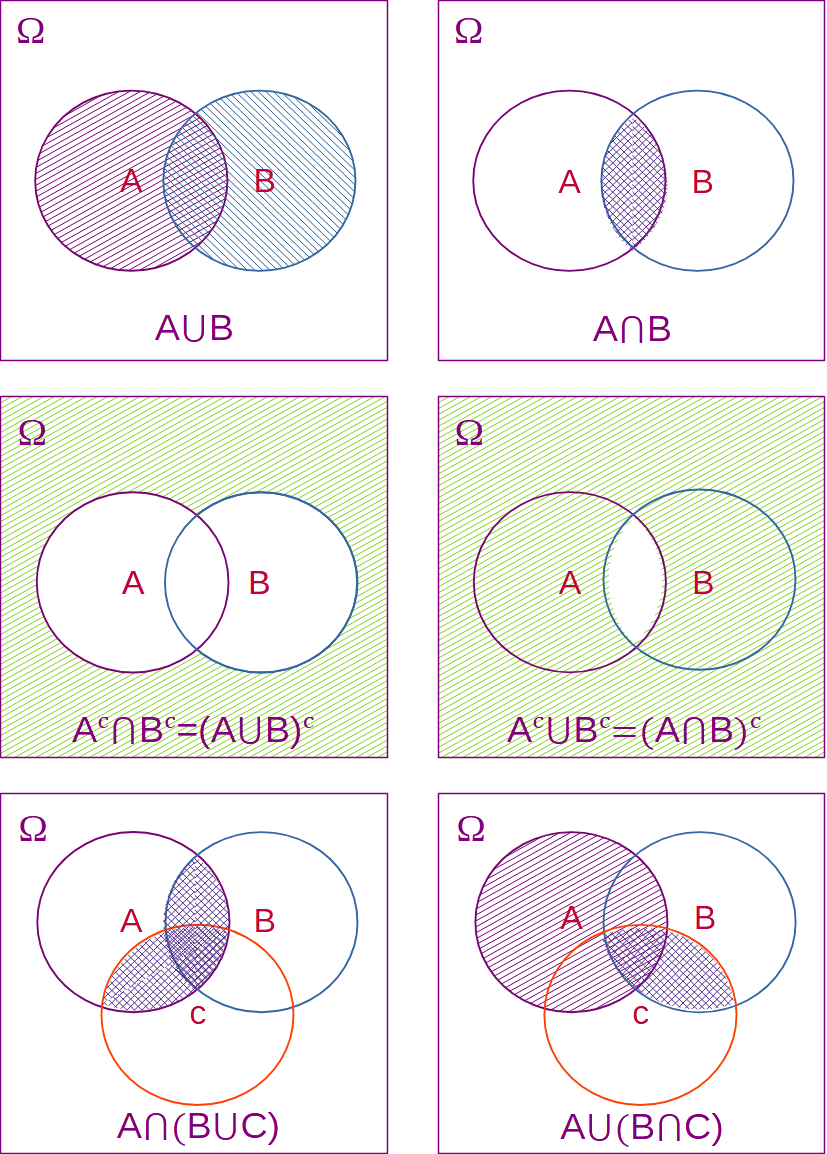
\includegraphics[width=5.30208in,height=\textheight]{Vennd.png}

}

\caption{\label{fig-venn}Diagramas de Venn}

\end{figure}%

Algunas de las leyes del álgebra de conjuntos se ilustran en los
diagramas de Venn en la Figura~\ref{fig-venn}. Aunque se utilizará
libremente cualquiera de las leyes mencionadas, podría resultar
instructivo proporcionar una prueba de una de ellas para ilustrar la
técnica. Se considera el siguiente ejemplo:

\begin{tcolorbox}[enhanced jigsaw, breakable, colbacktitle=quarto-callout-caution-color!10!white, rightrule=.15mm, toptitle=1mm, colback=white, left=2mm, colframe=quarto-callout-caution-color-frame, bottomtitle=1mm, opacitybacktitle=0.6, leftrule=.75mm, arc=.35mm, title={Ejemplo}, coltitle=black, titlerule=0mm, opacityback=0, bottomrule=.15mm, toprule=.15mm]

Demostrar que \((A \cup B)^c = A^c \cap B^c\).

\begin{proof}
Según la definición, dos conjuntos son iguales si cada uno está
contenido en el otro. Primero se demuestra que
\((A\cup B)^c \subset A^c\cap B^c\) al probar que si
\(\omega \in (A\cup B)^c\), entonces \(\omega \in A^c \cap B^c\). Ahora
bien, \(\omega \in (A\cup B)^c\) implica que \(\omega \notin A \cup B\),
lo cual implica que \(\omega \notin A\) y \(\omega \notin B\), lo que a
su vez implica que \(\omega \in A^c\) y \(\omega \in B^c\); es decir,
\(\omega \in A^c\cap B^c\). A continuación se demuestra que
\(A^c \cap B^c \subset (A\cup B)^c\). Sea \(\omega \in A^c \cap B^c\),
lo que significa que \(\omega\) pertenece tanto a \(A^c\) como a
\(B^c\). Entonces, \(\omega \notin A \cup B\), ya que de lo contrario
\(\omega\) debería pertenecer al menos a uno de los conjuntos \(A\) o
\(B\), lo cual contradice que \(\omega\) pertenezca tanto a \(A^c\) como
a \(B^c\); sin embargo, \(\omega \notin A \cup B\) implica que
\(\omega \in (A\cup B)^c\), lo que completa la prueba.
\end{proof}

\end{tcolorbox}

Se han introducido la unión y la intersección de dos conjuntos; estas
definiciones se extienden inmediatamente a más de dos conjuntos, de
hecho, a un número arbitrario de conjuntos. Es costumbre distinguir
entre los conjuntos en una colección de subconjuntos de \(\Omega\)
asignándoles nombres en forma de subíndices.

Se considera el conjunto de índices \(\Lambda\) como el catálogo de
nombres o índices. A \(\Lambda\) también se le denomina conjunto de
índices. Por ejemplo, si se tiene interés únicamente en dos conjuntos,
entonces el conjunto de índices \(\Lambda\) incluye solo dos índices,
por ejemplo, 1 y 2; así, \(\Lambda=\{1,2\}\).

\begin{definition}[Unión e intersección de
conjuntos]\protect\hypertarget{def-UI}{}\label{def-UI}

Sea \(\Lambda\) un conjunto de índices y
\(\{A_\lambda: \lambda \in \Lambda\}= \{A_\lambda\}\), una colección de
subconjuntos de \(\Omega\) indexados por \(\Lambda\). El conjunto de
puntos que consiste en todos los puntos que pertenecen a \(A_\lambda\)
para al menos un \(\lambda\) se denomina unión de los conjuntos
\(\{A_\lambda\}\) y se denota como
\(\bigcup\limits_{\lambda\in \Lambda} A_\lambda\). El conjunto de puntos
que consiste en todos los puntos que pertenecen a \(A_\lambda\) para
cada \(\lambda\) se denomina intersección de los conjuntos
\(\{A_\lambda\}\) y se denota como
\(\bigcap\limits_{\lambda\in\Lambda} A_\lambda\). Si \(\Lambda\) está
vacío, entonces se define
\(\bigcup\limits_{\lambda\in \Lambda} A_\lambda = \emptyset\) y
\(\bigcap\limits_{\lambda\in\Lambda} A_\lambda=\Omega\).

\end{definition}

Uno de los teoremas fundamentales que relaciona las uniones,
intersecciones y complementos para una colección arbitraria de conjuntos
se debe a De Morgan.

\begin{theorem}[Teorema de De
Morgan]\protect\hypertarget{thm-morgan}{}\label{thm-morgan}

Sea \(\Lambda\) un conjunto de índices y \(\{A_\lambda\}\) una colección
de subconjuntos de \(\Omega\) indexados por \(\Lambda\). Entonces,

\begin{enumerate}
\def\labelenumi{\roman{enumi}.}
\item
  \(\left(\bigcup\limits_{\lambda\in\Lambda} A_\lambda\right)^c = \bigcap\limits_{\lambda\in\Lambda} A_\lambda^c\)
\item
  \(\left(\bigcap\limits_{\lambda\in\Lambda} A_\lambda\right)^c = \bigcup\limits_{\lambda\in\Lambda} A_\lambda^c\)
\end{enumerate}

\end{theorem}

\begin{definition}[Disjuntos o mutuamente
excluyentes]\protect\hypertarget{def-disjunto}{}\label{def-disjunto}

Los subconjuntos \(A\) y \(B\) de \(\Omega\) se definen como mutuamente
excluyentes o disjuntos si \(A\cap B=\emptyset\). Los subconjuntos
\(A_1, A_2, \ldots\) se definen como mutuamente excluyentes si
\(A_i\cap A_j=\emptyset\) para cada \(i\neq j\).

\end{definition}

\chapter{Probabilidad}\label{probabilidad}

Una de las herramientas fundamentales de la estadística es la
probabilidad, la cual tuvo sus inicios formales con los juegos de azar
en el siglo XVII. Los juegos de azar, como su nombre indica, involucran
acciones como girar una rueda de ruleta, lanzar dados, lanzar una
moneda, sacar una carta, entre otros, en los que el resultado de un
evento es incierto. No obstante, se reconoce que aunque el resultado de
cada evento en particular pueda ser incierto, existe un patrón
predecible a largo plazo. Por ejemplo, se sabe que en múltiples
lanzamientos de una moneda ideal (equilibrada y simétrica),
aproximadamente la mitad de los resultados serán caras. Es esta
regularidad predecible a largo plazo la que permite a las casas de juego
mantener sus negocios.

Un tipo similar de incertidumbre y regularidad a largo plazo se observa
con frecuencia en la ciencia experimental. Por ejemplo, en la ciencia de
la genética no se puede determinar con certeza si una descendencia será
masculina o femenina, pero a largo plazo se sabe aproximadamente qué
porcentaje de descendencia será de cada sexo. De manera análoga, una
compañía de seguros de vida no puede predecir qué personas en los
Estados Unidos morirán a los 50 años, pero puede hacer predicciones
precisas sobre cuántas personas morirán a esa edad en promedio.

Para brindar una idea de lo que es la probabilidad, (Mood, Graybill, y
Boes 1986) proporciona las siguientes definiciones:

\begin{definition}[Probabilidad
clásica]\protect\hypertarget{def-pclas}{}\label{def-pclas}

Si un experimento aleatorio puede resultar en \(n\) resultados
mutuamente excluyentes e igualmente probables y si \(s\) de estos
resultados tienen un atributo \(A\), entonces la probabilidad de \(A\)
es la fracción \(s/n\).

\end{definition}

\begin{definition}[Probabilidad
frecuentista]\protect\hypertarget{def-pfrec}{}\label{def-pfrec}

Suponiendo que después de \(n\) repeticiones, para valores muy grandes
de \(n\), un evento \(A\) puede ocurrir \(s\) veces. Entonces \(p=s/n\).

\end{definition}

Estas definiciones, a pesar de su intuición, presentan limitaciones
significativas. Por ejemplo, la primera definición es circular, ya que
la frase ``igualmente probables'' es justamente lo que se intenta
definir. Además, la segunda definición no especifica los valores de
\(n\), lo cual puede generar ambigüedad. Estas definiciones son
consideradas antiguas, pero aún pueden brindar una comprensión general
del concepto de \textbf{probabilidad}.

\section{Espacio muestral y eventos}\label{espacio-muestral-y-eventos}

A continuación, se presentarán algunas definiciones que resultarán de
gran utilidad para adquirir un mayor conocimiento sobre el concepto de
probabilidad. Se usará como referencia (Lipschutz 1996).

\begin{definition}[Espacio
muestral]\protect\hypertarget{def-espm}{}\label{def-espm}

El espacio muestral, denotado por \(\Omega\), es la colección o
totalidad de todos los posibles resultados de un experimento conceptual.

\end{definition}

Un resultado particular, es decir, un elemento del espacio muestral
\(\Omega\), se denomina un \textbf{\emph{punto muestral}} o una
\textbf{\emph{muestra}}.

\begin{definition}[Evento]\protect\hypertarget{def-evento}{}\label{def-evento}

Un evento \(A\) es un subconjunto del espacio muestral \(\Omega\), es
decir, es un conjunto de resultados.

\end{definition}

\begin{definition}[Espacio de
eventos]\protect\hypertarget{def-espev}{}\label{def-espev}

La clase de todos los eventos asociados a un experimento dado se define
como el espacio de eventos y se denotará por \(\mathfrak{F}\).

\end{definition}

\begin{definition}[Evento
particular]\protect\hypertarget{def-evpart}{}\label{def-evpart}

El evento \(\{\omega\}\), que está constituido por un solo punto
\(\omega \in \Omega\), se denomina \emph{evento muestral} o \emph{punto
muestral}.

\end{definition}

Las definiciones anteriores no definen con precisión lo que es un
evento, ya que aunque un evento siempre será un subconjunto del espacio
muestral, en espacios muestrales suficientemente grandes, no todos los
subconjuntos serán eventos. Por lo tanto, la clase de todos los
subconjuntos del espacio muestral no necesariamente corresponderá al
espacio de eventos. Sin embargo, se observará que la clase de todos los
eventos siempre se puede seleccionar lo suficientemente grande como para
incluir todos aquellos subconjuntos (eventos) cuya probabilidad se desee
analizar. Si el espacio muestral consta solo de un número finito de
puntos, entonces el espacio de eventos correspondiente será la clase de
todos los subconjuntos del espacio muestral.

Los conceptos presentados se ilustran con unos ejemplos muy simples;

\begin{tcolorbox}[enhanced jigsaw, breakable, colbacktitle=quarto-callout-caution-color!10!white, rightrule=.15mm, toptitle=1mm, colback=white, left=2mm, colframe=quarto-callout-caution-color-frame, bottomtitle=1mm, opacitybacktitle=0.6, leftrule=.75mm, arc=.35mm, title={Ejemplo (\textbf{\emph{Lanzamiento de una moneda}})}, coltitle=black, titlerule=0mm, opacityback=0, bottomrule=.15mm, toprule=.15mm]

Considere el experimento de lanzar una moneda una vez, este experimento
es uno de los más sencillos, pero permite representar claramente los
conceptos. El espacio muestral estaría conformado por
\(\Omega = \{A, S\}\), donde \(A\) representa el resultado de que caiga
águila y \(S\) representa el resultado de que caiga sol. El conjunto
\(\mathfrak{F}\) está representado por \(\{\{A\}, \{S\}\}\), el cuál
también es un subconjunto de \(\Omega\).

Es importante destacar que el conjunto vacío \(\emptyset\) y el conjunto
completo \(\Omega\) también son subconjuntos de \(\Omega\), pero
generalmente no se consideran eventos de interés en este contexto.

\end{tcolorbox}

\begin{tcolorbox}[enhanced jigsaw, breakable, colbacktitle=quarto-callout-caution-color!10!white, rightrule=.15mm, toptitle=1mm, colback=white, left=2mm, colframe=quarto-callout-caution-color-frame, bottomtitle=1mm, opacitybacktitle=0.6, leftrule=.75mm, arc=.35mm, title={Ejemplo (\textbf{\emph{Lanzamiento de un dado}})}, coltitle=black, titlerule=0mm, opacityback=0, bottomrule=.15mm, toprule=.15mm]

Considerando el experimento de lanzar un dado de \(6\) caras, el espacio
muestral \(\Omega\) se define como

\[ \Omega = \{1,2,3,4,5,6\}. \]

Un punto muestral podría ser un resultado específico, por ejemplo,
\(\{1\}\). Todos los subconjuntos posibles de resultados constituirían
el conjunto \(\mathfrak{F}\). Se definen los eventos \(A\), que
representa el evento de obtener un resultado par; \(B\), que representa
el evento de obtener un resultado impar; y \(C\), que representa el
evento de obtener un resultado mayor a 3. Por lo tanto, se tiene:

\[ A= \{2,4,6\},\quad B=\{1,3,5\},\quad C=\{4,5,6\}. \]

Se observa que el evento de la unión de los eventos \(B\) y \(C\),
denotado como \(B\cup C\), es igual a \(\{1, 3, 4, 5, 6\}\), el cual
también es un evento en el espacio muestral \(\Omega\). Finalmente, se
destaca que los eventos \(A\) y \(B\) no tienen elementos en común, es
decir, \(A \cap B = \emptyset\). Por lo tanto, se dice que estos eventos
son ajenos, mutuamente excluyentes o disjuntos.

\end{tcolorbox}

La definición de espacio muestral es precisa y satisfactoria, mientras
que las definiciones de evento y espacio de eventos no son completamente
satisfactorias. Se mencionó que si el espacio muestral era
``suficientemente grande'', no todos los subconjuntos del espacio
muestral serían eventos; sin embargo, no se especificó exactamente qué
subconjuntos serían eventos y cuáles no lo serían. En lugar de
desarrollar las matemáticas necesarias para definir con precisión qué
subconjuntos de \(\Omega\) constituyen nuestro espacio de eventos
\(\mathfrak{F}\), se pueden enunciar algunas propiedades de
\(\mathfrak{F}\) que parecen razonables requerir.

\begin{enumerate}
\def\labelenumi{\roman{enumi}.}
\item
  \(\Omega \in \mathfrak{F}\).
\item
  Si \(A\in\mathfrak{F}\), entonces \(A^c\in \mathfrak{F}\).
\item
  Si \(A_1\) y \(A_2\in \mathfrak{F}\), entonces
  \(A_1\cup A_2\in \mathfrak{F}\).
\end{enumerate}

Se mencionó anteriormente que el interés principal radica en los eventos
debido a la probabilidad de que ocurran. Por lo tanto, es deseable que
\(\mathfrak{F}\) incluya \(\Omega\), el evento seguro. Además, si \(A\)
es un evento, lo que significa que se puede hablar sobre la probabilidad
de que ocurra \(A\), entonces \(A^c\) también debería ser un evento para
poder hablar sobre la probabilidad de que \(A\) no ocurra. De manera
similar, si \(A_1\) y \(A_2\) son eventos, entonces \(A_1\cup A_2\)
también debería ser un evento.

Cualquier colección de eventos con propiedades (i.) y (iii.) se denomina
álgebra booleana, o simplemente álgebra, de eventos. Cabe señalar que la
colección de todos los subconjuntos de \(\Omega\) satisface
necesariamente las propiedades mencionadas anteriormente. Varios
resultados se derivan de las propiedades asumidas anteriormente de
\(\mathfrak{F}\).

\section{Definición de
probabilidad}\label{definiciuxf3n-de-probabilidad}

En esta sección se presenta la definición axiomática de probabilidad.
Aunque esta definición formal de probabilidad, por sí sola, no permite
asignar probabilidades reales a eventos que consisten en ciertos
resultados de experimentos aleatorios, es otra de una serie de
definiciones que conducen a ese objetivo. Dado que la probabilidad, al
igual que los conceptos que se presentarán, se define como una función
particular, se inicia esta subsección con una revisión del concepto de
función.

\begin{definition}[Función]\protect\hypertarget{def-funcion}{}\label{def-funcion}

Una función, llamada \(f(\cdot)\), con dominio \(A\) y contradominio
\(B\), es una colección de pares ordenados, llamados \((a,b)\), que
cumplen las siguientes condiciones:

\begin{enumerate}
\def\labelenumi{\roman{enumi}.}
\item
  \(a\in A\) y \(b\in B\)
\item
  Cada \(a\in A\) aparece como el primer elemento de algún par ordenado
  en la colección (cada \(b\in B\) no necesariamente es el segundo
  elemento de algún par ordenado)
\item
  Ningún par ordenado en la colección tiene el mismo primer elemento que
  otro par ordenado distinto.
\end{enumerate}

\end{definition}

Si \((a,b)\in f(\cdot)\), se escribe \(b=f(a)\) (se lee ``\(b\) es igual
a \(f\) de \(a\)'') y se denomina \(f(a)\) como el valor de \(f(\cdot)\)
en \(a\). Para cualquier \(a\in A\), \(f(a)\) es un elemento de \(B\);
mientras que \(f(\cdot)\) es un conjunto de pares ordenados. El conjunto
de todos los valores de \(f(\cdot)\) se denomina rango de \(f(\cdot)\);
es decir, el rango de
\(f(\cdot)=\{b\in B:b=f(a) \text{ para algún } a\in A\}\) y siempre es
un subconjunto del contradominio \(B\), pero no necesariamente igual a
él. \(f(a)\) también se denomina imagen de \(a\) bajo \(f(\cdot)\), y
\(a\) se denomina preimagen de \(f(a)\).

\begin{tcolorbox}[enhanced jigsaw, breakable, colbacktitle=quarto-callout-caution-color!10!white, rightrule=.15mm, toptitle=1mm, colback=white, left=2mm, colframe=quarto-callout-caution-color-frame, bottomtitle=1mm, opacitybacktitle=0.6, leftrule=.75mm, arc=.35mm, title={Ejemplo}, coltitle=black, titlerule=0mm, opacityback=0, bottomrule=.15mm, toprule=.15mm]

Sean \(f_1(\cdot)\) y \(f_2(\cdot)\) dos funciones con la recta real
como su dominio y contradominio, definidas por

\[ f_1(\cdot)=\{(x,y): y=x^3+1, -\infty< x< \infty\} \]

y

\[ f_2(\cdot)=\{(x,y): y=x^2, -\infty<x< \infty\} \]

El rango de \(f_1(\cdot)\) es el contradominio, que es toda la recta
real, pero el rango de \(f_2(\cdot)\) son todos los números reales no
negativos, que no es igual al contradominio.

\end{tcolorbox}

De particular interés será una clase de funciones conocidas como
funciones indicadoras.

\begin{definition}[Función
indicadora]\protect\hypertarget{def-f_ind}{}\label{def-f_ind}

Sea \(\Omega\) cualquier espacio con puntos \(\omega\) y \(A\) cualquier
subconjunto de \(\Omega\). La función indicadora de \(A\), denominada
\(I_A(\cdot)\), es la función con dominio \(\Omega\) y contradominio
formado por dos números reales, 0 y 1, definida por

\[ I_A(\omega)= \left\{\begin{array}{lcc} 1 & si & \omega \in A\\ \\0 & si & \omega \notin A \end{array}\right. \]

\(I_A(\cdot)\) claramente ``indica'' el conjunto \(A\).

\end{definition}

\textbf{\emph{Propiedades de la función indicadora.}}

Sea \(\Omega\) cualquier espacio y \(\mathfrak{F}\) cualquier colección
de subconjuntos de \(\Omega\):

\begin{enumerate}
\def\labelenumi{\roman{enumi}.}
\item
  \(I_A(\omega)= 1- I_{A^c}(\omega)\) para cada \(A\in \mathfrak{F}\).
\item
  \(I_{A_1A_2\cdots A_n}(\omega)= I_{A_1}(\omega)\cdot I_{A_2}(\omega)\cdots I_{A_n}(\omega)\)
  para \(A_1,\ldots, A_n\in \mathfrak{F}\).
\item
  \(I_{A_1\cup A_2\cup\cdots\cup A_n}(\omega)= \max{[I_{A_1}(\omega), I_{A_2}(\omega),\ldots, I_{A_n}(\omega)]}\)
  para \(A_1, \ldots, A_n \in\mathfrak{F}\).
\item
  \(I_A^2(\omega)= I_A(\omega)\) para cada \(A\in\mathfrak{F}\).
\end{enumerate}

La función indicadora será utilizada para ``indicar'' subconjuntos de la
recta real. Por ejemplo:

\[I_{\{[0,1)\}}(x)= I_{[0,1)}(x)=\begin{cases} 1 & \text{si }\quad 0\leq x<1,\\ \\ 0 & \text{otro caso.} \end{cases} \]

Si \(I^+\) denota el conjunto de números enteros positivos,

\[ I_{I^+}(X)=\begin{cases} 1 & \text{si $x$ es algún entero positivo,}\\ \\ 0 & \text{otro caso.}\end{cases}\]

Otro tipo de función del cual se tendrá ocasión de discutir es la
función de conjunto definida como cualquier función que tiene como
dominio una colección de conjuntos y como contradominio la recta real,
incluyendo posiblemente el infinito. A continuación se muestra un
ejemplo de función de conjunto.

\begin{tcolorbox}[enhanced jigsaw, breakable, colbacktitle=quarto-callout-caution-color!10!white, rightrule=.15mm, toptitle=1mm, colback=white, left=2mm, colframe=quarto-callout-caution-color-frame, bottomtitle=1mm, opacitybacktitle=0.6, leftrule=.75mm, arc=.35mm, title={Ejemplo}, coltitle=black, titlerule=0mm, opacityback=0, bottomrule=.15mm, toprule=.15mm]

Sea \(\Omega\) el espacio muestral correspondiente al experimento de
lanzar dos dados, y sea \(\mathfrak{F}\) la colección de todos los
subconjuntos de \(\Omega\). Para cualquier \(A\in\mathfrak{F}\), se
define \(N(A)\) como el número de resultados, o puntos en \(\Omega\),
que están en \(A\). Entonces, \(N(\emptyset)=0\), \(N(\Omega)=36\) y
\(N(A)=6\) si \(A\) es el evento que contiene aquellos resultados que
tienen un total de siete puntos arriba.

\end{tcolorbox}

La función de tamaño del conjunto aludida en el ejemplo anterior puede
ser definida, en general, para cualquier conjunto \(A\) como el número
de puntos en \(A\), donde \(A\) es un miembro de una colección
arbitraria de conjuntos \(\mathfrak{F}\).

La función de probabilidad que se definirá será una función de conjunto
particular.

\begin{definition}[Función de
probabilidad]\protect\hypertarget{def-fprob}{}\label{def-fprob}

Sea \(A\) un evento del espacio muestral \(\Omega\). Una función
\(P: \mathfrak{F} \to [0,1]\) es llamada función de probabilidad y
\(P(A)\) se denomina la \emph{probabilidad} del evento \(A\) si se
cumplen los siguientes axiomas:

\begin{enumerate}
\def\labelenumi{\roman{enumi}.}
\item
  \textbf{\emph{No negatividad}}: Para todo evento \(A\) en
  \(\mathfrak{F}\), la probabilidad \(P(A)\) es un número no negativo,
  es decir, \(P(A) \geq 0\).
\item
  \textbf{\emph{Probabilidad unitaria}}: La probabilidad del espacio
  muestral completo \(\Omega\) es igual a 1, es decir,
  \(P(\Omega) = 1\).
\item
  \textbf{\emph{Aditividad}}: Para cualquier colección de eventos
  mutuamente excluyentes \(A_1, A_2, A_3, \ldots\), la probabilidad de
  la unión de estos eventos es igual a la suma de las probabilidades
  individuales, es decir,
  \[P\left(\bigcup_{i=1}^\infty A_i\right) = \sum_{i=1}^\infty P(A_i).\]
\end{enumerate}

\end{definition}

Estos axiomas establecen las propiedades esenciales que debe cumplir una
función de probabilidad para ser considerada válida. Cumplir con estos
axiomas garantiza que la función de probabilidad asigna valores
coherentes y consistentes a los eventos en el espacio muestral.

A partir de los axiomas, se derivan otras propiedades que ayudan a
calcular las probabilidades de varios eventos.

\begin{enumerate}
\def\labelenumi{\roman{enumi}.}
\item
  \(P(\emptyset)=0\).
\item
  Si \(A_1, \ldots, A_n\) son eventos mutuamente excluyentes en
  \(\mathfrak{F}\), entonces
  \[P\left(\bigcup\limits_{i=1}^n A_i\right)= \sum\limits_{i=1}^n P(A_i).\]
\item
  Si \(A\) es un evento en \(\mathfrak{F}\), entonces
  \[P(A^c)= 1-P(A).\]
\item
  Si \(A,B\in\mathfrak{F}\), entonces

  \[P(A)= P(A\cap B)+ P(A\cap B^c)\]

  y \[P(A-B)=P(A\cap B^c)= P(A)-P(A\cap B).\]
\item
  Si \(A,B\in \mathfrak{F}\) y \(A\subset B\), entonces
  \(P(A)\leq P(B)\).
\item
  Para cualesquiera dos eventos \(A,B\in \mathfrak{F}\);
  \[P(A\cup B)= P(A)+P(B)-P(A\cap B).\]Más generalmente, para eventos
  \(A_1, A_2, \ldots, A_n\in \mathfrak{F}\)
\end{enumerate}

\[ \begin{split}P\left(\bigcup\limits_{i=1}^n A_i\right) & = \sum_{j=1}^nP(A_j)-{\sum\sum}_{i<j} P(A_i\cap A_j)\\ &+\sum\sum\sum_{i<j<k}P(A_i\cap A_j\cap A_k) -\cdots+(-1)^{n+1}P(A_1\cap \ldots\cap A_n).\end{split} \]

\begin{theorem}[Desigualdad de
Boole]\protect\hypertarget{thm-boole}{}\label{thm-boole}

Si \(A_1, A_2, \ldots, A_n\in\mathfrak{F}\), entonces

\[P\left(\bigcup_{i=1}^n A_i\right)\leq \sum_{i=1}^n P(A_i).\]

\end{theorem}

Finalmente se concluye esta subsección con la siguiente definición;

\begin{definition}[Espacio de
probabilidad]\protect\hypertarget{def-Ep}{}\label{def-Ep}

Un espacio de probabilidad es la terna \((\Omega, \mathfrak{F}, P)\),
donde \(\Omega\) es un espacio muestral, \(\mathfrak{F}\) es una
colección (asumida como un álgebra) de eventos (cada uno un subconjunto
de \(\Omega\)), y \(P\) es una función de probabilidad con dominio
\(\mathfrak{F}\).

\end{definition}

\section{Probabilidad condicional}\label{probabilidad-condicional}

En ocasiones, es de interés conocer la probabilidad de un evento, dado
que haya ocurrido otro. En este sentido, se define la probabilidad
condicional.

\begin{definition}[Probabilidad
condicional]\protect\hypertarget{def-pcond}{}\label{def-pcond}

Sean \(A\) y \(B\) dos eventos en \(\mathfrak{F}\) del espacio de
probabilidad dado \((\Omega, \mathfrak{F}, P)\). La probabilidad
condicional del evento \(A\) dado el evento \(B\), denotada por
\(P(A|B)\), se define como sigue;

\[P(A|B)= \frac{P(A\cap B)}{P(B)}\qquad\text{si }\quad P(B)>0.\]

En caso de que \(P(B)=0\) se deja sin definir.

\end{definition}

\begin{remark}
Una fórmula que es evidente a partir de la definición es
\[P(A\cap B)= P(A|B)P(B)=P(B|A)P(A)\] si tanto \(P(A)\) como \(P(B)\)
son diferentes de cero. Esta fórmula relaciona \(P(A|B)\) con \(P(B|A)\)
en términos de las probabilidades incondicionales \(P(A)\) y \(P(B)\).
\end{remark}

De la definición anterior, se desprenden las siguientes propiedades de
la función de probabilidad condicional. Se asume que el espacio de
probabilidad \((\Omega, \mathfrak{F}, P)\) está dado, y se considera que
\(B\in\mathfrak{F}\) cumple con \(P(B)>0\).

\begin{enumerate}
\def\labelenumi{\roman{enumi}.}
\item
  \(P(\emptyset| B)=0\).
\item
  Si \(A_1, A_2, \ldots, A_n\) son eventos mutuamente excluyentes en
  \(\mathfrak{F}\), entonces

  \[P\left(\bigcup_{i=1}^n A_i|B\right)= \sum_{i=1}^n P(A_i|B).\]
\item
  Si \(A\) es un evento en \(\mathfrak{F}\), entonces
  \(P(A^c| B)=1-P(A|B)\).
\item
  Si \(A_1, A_2\in \mathfrak{F}\), entonces
  \(P(A_1|B)=P(A_1\cap A_2|B)+ P(A_1\cap A_2^c|B)\).
\item
  Para cualesquiera dos eventos \(A_1,A_2\in \mathfrak{F}\)

  \[P(A_1\cup A_2|B)=P(A_1|B)+P(A_2|B)-P(A_1\cap A_2|B).\]
\item
  Si \(A_1, A_2\in\mathfrak{F}\) y \(A_1\subset A_2\), entonces
  \(P(A_1|B)\leq P(A_2|B)\).
\item
  Si \(A_1, A_2,\ldots, A_n\in\mathfrak{F}\), entonces

  \[P\left(\bigcup_{i=1}^n A_i|B\right)\leq \sum_{i=1}^n P(A_i|B).\]
\end{enumerate}

A continuación se mencionan unos teoremas de gran importancia. La
aplicación de dichos teoremas se ilustran con unos ejemplos.

\begin{theorem}[Teorema de probabilidades
totales]\protect\hypertarget{thm-ptotales}{}\label{thm-ptotales}

Para un espacio de probabilidad dado \((\Omega, \mathfrak{F}, P)\), si
\(B_1, B_2, \ldots, B_n\) es una colección de eventos mutuamente
disjuntos en \(\mathfrak{F}\) que satisfacen
\(\Omega = \bigcup\limits_{j=1}^n B_j\) y \(P(B_j)>0\) para
\(j=1,\ldots, n\), entonces para cada \(A\in \mathfrak{F}\),
\[P(A)=\sum_{j=1}^n P(A|B_j)P(B_j).\]

\begin{proof}
Se observa que \(A=\bigcup\limits_{j=1}^n A\cap B_j\) y los conjuntos
\(A\cap B_j\) son mutuamente disjuntos; por lo tanto,

\[P(A)=P\left(\bigcup_{j=1}^n A\cap B_j\right)=\sum_{j=1}^n P(A\cap B_j)= \sum_{j=1}^n P(A|B_j)P(B_j).\]
\end{proof}

\end{theorem}

\begin{tcolorbox}[enhanced jigsaw, breakable, colbacktitle=quarto-callout-caution-color!10!white, rightrule=.15mm, toptitle=1mm, colback=white, left=2mm, colframe=quarto-callout-caution-color-frame, bottomtitle=1mm, opacitybacktitle=0.6, leftrule=.75mm, arc=.35mm, title={Ejemplo (\textbf{\emph{Seleccionar una pelota de varias urnas}})}, coltitle=black, titlerule=0mm, opacityback=0, bottomrule=.15mm, toprule=.15mm]

Hay dos urnas con pelotas de diferentes colores, todas del mismo tamaño.
En la primera urna, hay tres pelotas rojas, tres blancas y cuatro
negras; en la segunda urna, hay cuatro pelotas rojas, tres blancas y una
negra. Se elige una urna al azar y se saca una pelota de ella. ¿Cuál es
la probabilidad de que la pelota extraída sea blanca?

\begin{solution}
Se debe observar que la elección de las urnas constituye dos eventos
mutuamente excluyentes, ya que la unión de ambos eventos constituye el
espacio muestral (todas las pelotas están en la primera o segunda urna).
Se denomina \(B_1\) al evento de seleccionar la primera urna, y \(B_2\)
al evento de seleccionar la segunda urna.

El evento de extraer una pelota blanca puede tener lugar tanto al elegir
la primera urna como al elegir la segunda urna, lo que permite la
aplicación de la fórmula del teorema de probabilidades totales. Se
designa como \(A\) al evento de seleccionar una pelota blanca.

De esta manera,

\[ P(A)= \sum_{j=1}^2 P(A|B_j)P(B_j)=P(A|B_1)P(B_1)+P(A|B_2)P(B_2) \]

Bajo la premisa de probabilidades equivalentes, se tiene que
\(P(B_1)=P(B_2)=\frac{1}{2}\), \(P(A|B_1)=\frac{3}{10}\) y
\(P(A|B_2)=\frac{3}{8}\), por lo que la probabilidad de elegir una
pelota blanca es \(0.3375\).
\end{solution}

\end{tcolorbox}

\begin{theorem}[Teorema de
Bayes]\protect\hypertarget{thm-bayes}{}\label{thm-bayes}

Para un espacio de probabilidad dado \((\Omega, \mathfrak{F}, P)\), si
\(B_1, B_2, \ldots, B_n\) es una colección de eventos mutuamente
disjuntos en \(\mathfrak{F}\) que satisfacen
\(\Omega=\bigcup\limits_{j=1}^n B_j\) y \(P(B_j)>0\) para
\(j=1,\ldots, n\), entonces para cada \(A\in\mathfrak{F}\) para el cual
\(P(A)>0\),

\[P(B_k|A)= \frac{P(A|B_k)P(B_k)}{\sum\limits_{j=1}^n P(A|B_j)P(B_j)}.\]

\begin{proof}
Utilizando tanto la definición de probabilidad condicional como el
teorema de probabilidad total, se sigue que

\[P(B_k|A)= \frac{P(B_k\cap A)}{P(A)}=\frac{P(A|B_k)P(B_k)}{\sum\limits_{j=1}^n P(A|B_j)P(B_j)}.\]

utilizando tanto la definición de probabilidad condicional como el
teorema de probabilidad total.
\end{proof}

\end{theorem}

\begin{tcolorbox}[enhanced jigsaw, breakable, colbacktitle=quarto-callout-caution-color!10!white, rightrule=.15mm, toptitle=1mm, colback=white, left=2mm, colframe=quarto-callout-caution-color-frame, bottomtitle=1mm, opacitybacktitle=0.6, leftrule=.75mm, arc=.35mm, title={Ejemplo (\textbf{\emph{Seleccionar una pelota de varias urnas}})}, coltitle=black, titlerule=0mm, opacityback=0, bottomrule=.15mm, toprule=.15mm]

Considérese el problema de las urnas. Teniendo en cuenta que la pelota
extraída fue blanca, ¿cuál es la probabilidad de que haya provenido de
la primera urna?

\begin{solution}
Debe calcularse la probabilidad \(P(B_1|A)\). Al utilizar el teorema de
Bayes, solo se realiza la sustitución en la fórmula y se obtiene que la
probabilidad resultante es \(0.4444\).
\end{solution}

\end{tcolorbox}

\begin{theorem}[Regla de
multiplicación]\protect\hypertarget{thm-mult}{}\label{thm-mult}

Para un espacio de probabilidad dado \((\Omega, \mathfrak{F}, P)\), sean
\(A_1, A_2, \ldots, A_n\) eventos pertenecientes a \(\mathfrak{F}\) para
los cuales \(P(A_1\cdots A_{n-1})>0\); entonces

\[P(A_1A_2\cdots A_n)= P(A_1)P(A_2|A_1)P(A_3|A_1A_2)\cdots P(A_n|A_1\cdots A_{n-1})\]

\end{theorem}

\section{Independencia de eventos}\label{independencia-de-eventos}

Si \(P(A|B)\) no depende del evento \(B\), es decir, \(P(A|B)=P(A)\),
entonces parecería natural decir que el evento \(A\) es independiente
del evento \(B\). Esto se establece en la siguiente definición.

\begin{definition}[Eventos
independientes]\protect\hypertarget{def-evind}{}\label{def-evind}

Para un espacio de probabilidad dado \((\Omega, \mathfrak{F}, P)\), sean
\(A\) y \(B\) dos eventos en \(\mathfrak{F}\). Los eventos \(A\) y \(B\)
se definen como \emph{independientes} si y solo si se cumple alguna de
las siguientes condiciones:

\begin{enumerate}
\def\labelenumi{\roman{enumi}.}
\item
  \(P(A\cap B)= P(A)P(B)\).
\item
  \(P(A|B)=P(A)\) si \(P(B)>0\).
\item
  \(P(B|A)=P(B)\) si \(P(A)>0\).
\end{enumerate}

\end{definition}

De la definición anterior, se desprende lo siguiente

\phantomsection\label{thm}
Si \(A\) y \(B\) son dos eventos independientes definidos en un espacio
de probabilidad dado \((\Omega, \mathfrak{F}, P)\), entonces los
siguientes eventos también son independientes

\begin{enumerate}
\def\labelenumi{\roman{enumi}.}
\item
  \(A\) y \(B^c\),
\item
  \(A^c\) y \(B\),
\item
  \(A^c\) y \(B^c\).
\end{enumerate}

\begin{remark}
No deben confundirse los términos \textbf{eventos independientes} y
\textbf{eventos disjuntos}. De hecho, los eventos disjuntos suelen ser
muy dependientes por que la ocurrencia de uno implica la no ocurrencia
del otro. El único evento que es independiente y ajeno es el vacío
\(\emptyset\).
\end{remark}

La noción de eventos independientes puede ser extendido a más de dos
eventos como se sigue;

\begin{definition}[Independencia de varios
eventos]\protect\hypertarget{def-ive}{}\label{def-ive}

Para un espacio de probabilidad dado \((\Omega, \mathfrak{F}, P)\), sean
\(A_1, A_2, \ldots, A_n\) eventos en \(\mathfrak{F}\). Los eventos
\(A_1, A_2, \ldots, A_n\) se definen como independientes si y solo si
\(P\left(\bigcap\limits_{i=1}^n A_i\right)=\prod\limits_{i=1}^n P(A_i)\).

\end{definition}

\section{Variables aleatorias}\label{variables-aleatorias}

Hasta el momento se conoce cómo asignar probabilidades a eventos del
espacio muestral, sin embargo, en la práctica esto no siempre es
posible, ya que sería complicado mencionar o enumerar todos los
elementos del espacio muestral.

Por esta razón, es necesario ``traducir'' dichos eventos a números
reales. Esto es posible mediante el uso de \emph{variables aleatorias}.

\begin{definition}[Variable
aleatoria]\protect\hypertarget{def-va}{}\label{def-va}

Para un espacio de probabilidad dado \((\Omega, \mathfrak{F}, P)\), una
variable aleatoria, denotada por \(X\) o \(X(\cdot)\), es una función
con dominio \(\Omega\) y contradominio la recta real. La función
\(X(\cdot)\) debe ser tal si \(\omega\in\Omega\) entonces
\(X(\omega)\in\mathbb R\). Si \(B\subset \mathbb R\) entonces
\(X^{-1}(B)\in\mathfrak{F}\), donde
\[X^{-1}(B)=\{\omega\in\Omega\ |\  X(\omega\in B)\}.\]

\end{definition}

Existen dos tipos de variables aleatorias: discretas y continuas. Las
variables aleatorias discretas toman sus valores en un conjunto finito o
numerable, por ejemplo, el conjunto de los números naturales
\(\mathbb N\). A este conjunto de valores se le conoce como conjunto de
valores posibles o \(D_X\). Las variables aleatorias continuas, por el
contrario, toman sus valores en el conjunto de los números reales
\(\mathbb R\).

\subsection{Función de
distribución}\label{funciuxf3n-de-distribuciuxf3n}

Para describir el comportamiento de una variable aleatoria, se debe
conocer cómo se comportan sus probabilidades, esto puede realizarse
mediante la \emph{función de distribución}.

\begin{definition}[Función de distribución
acumulada]\protect\hypertarget{def-fundist}{}\label{def-fundist}

La función de distribución acumulada de una variable aleatoria \(X\),
denotada por \(F_X(\cdot)\), se define como aquella función con dominio
la recta real y contradominio el intervalo \([0,1]\), que satisface
\(F_X(x)=P(X\leq x)=P({\omega: X(\omega)\leq x})\) para cada número real
\(x\).

\end{definition}

Una función de distribución definida es única para cada variable y
siempre existirá, es importante conocerla porque con ella se pueden
calcular probabilidades de la variable aleatoria.

A continuación, se presentan ejemplos y propiedades de la función de
distribución acumulada.

\begin{tcolorbox}[enhanced jigsaw, breakable, colbacktitle=quarto-callout-caution-color!10!white, rightrule=.15mm, toptitle=1mm, colback=white, left=2mm, colframe=quarto-callout-caution-color-frame, bottomtitle=1mm, opacitybacktitle=0.6, leftrule=.75mm, arc=.35mm, title={Ejemplo}, coltitle=black, titlerule=0mm, opacityback=0, bottomrule=.15mm, toprule=.15mm]

Se considera el experimento de lanzar una moneda. Supongamos que la
moneda es justa. Sea \(X\) el número de caras obtenidas. Entonces,

\[F_X(x)=\left\{ \begin{array}{lcc} 0 & \text{si} & x<0\\ \\ \frac{1}{2} & \text{si} & 0\leq x<1 \\ \\1 & \text{si} & 1\leq x \end{array} \right. \]

O \(F_X(x)=\frac{1}{2}I_{[0,1)}(x)+ I_{[1,\infty)}(x)\) en nuestra
notación de función indicadora.

\end{tcolorbox}

\subsubsection{\texorpdfstring{\textbf{\emph{Propiedades de la función
de distribución
acumulada.}}}{Propiedades de la función de distribución acumulada.}}\label{propiedades-de-la-funciuxf3n-de-distribuciuxf3n-acumulada.}

\begin{enumerate}
\def\labelenumi{\roman{enumi}.}
\item
  \(F_X(-\infty)\equiv \lim\limits_{x\to-\infty} F_X(x)=0\), y
  \(F_X(+\infty)\equiv \lim\limits_{x\to+\infty} F_X(x)=1\).
\item
  \(F_X(\cdot)\) es una función monótona creciente; es decir, para toda
  \(a< b\) entonces \(F_X(a)\leq F_X(b)\).
\item
  \(F_X(\cdot)\) es continua por la derecha, esto es
  \(\lim\limits_{0<h\to 0} F_X(x+h)=F_X(x)\).
\end{enumerate}

\begin{definition}[Función de distribución
acumulada]\protect\hypertarget{def-FDA}{}\label{def-FDA}

Cualquier función \(F(\cdot)\) con dominio la recta real y contradominio
el intervalo \([0,1]\), que satisface las tres propiedades mencionadas
anteriormente, se define como una función de distribución acumulada.

\end{definition}

\begin{tcolorbox}[enhanced jigsaw, breakable, colbacktitle=quarto-callout-caution-color!10!white, rightrule=.15mm, toptitle=1mm, colback=white, left=2mm, colframe=quarto-callout-caution-color-frame, bottomtitle=1mm, opacitybacktitle=0.6, leftrule=.75mm, arc=.35mm, title={Ejemplo (\textbf{\emph{Lanzar 3 monedas}})}, coltitle=black, titlerule=0mm, opacityback=0, bottomrule=.15mm, toprule=.15mm]

Considérese el ejemplo del lanzamiento de tres monedas. Sea \(X\) el
número de águilas en tres lanzamientos.

La función de distribución es la siguiente:

\[ F_X(x)=\begin{cases}0 & \text{ si } x<0,\\ \frac{1}{8} & \text{ si } 0\leq x< 1,\\ \frac{1}{2} & \text{ si  } 1\leq x< 2,\\ \frac{7}{8} & \text{ si  } 2\leq x<3,\\ 1 & \text{ si } 3\leq x.\end{cases} \]

A continuación se muestra una gráfica de la función

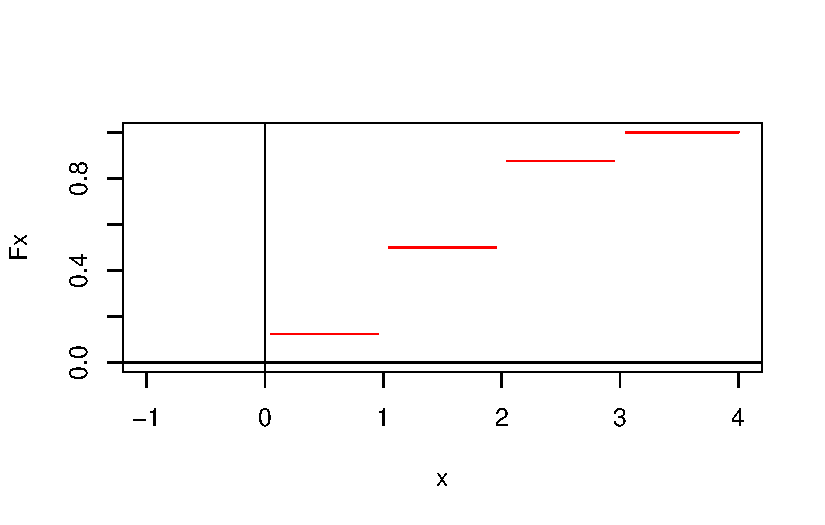
\includegraphics{probabilidad_files/figure-pdf/unnamed-chunk-1-1.pdf}

Por ejemplo, la probabilidad de que se obtenga 0 a 1 águilas es
\(\frac{1}{8}\).

\end{tcolorbox}

\begin{tcolorbox}[enhanced jigsaw, breakable, colbacktitle=quarto-callout-caution-color!10!white, rightrule=.15mm, toptitle=1mm, colback=white, left=2mm, colframe=quarto-callout-caution-color-frame, bottomtitle=1mm, opacitybacktitle=0.6, leftrule=.75mm, arc=.35mm, title={Ejemplo (\textbf{\emph{Duración de una llamada telefónica}})}, coltitle=black, titlerule=0mm, opacityback=0, bottomrule=.15mm, toprule=.15mm]

Para las variables aleatorias continuas, la forma de la función de
distribución es un poco distinta, pero sigue cumpliendo las mismas
propiedades.

A continuación se representa una función de distribución acumulada de la
variable aleatoria \(X\) que podría ser usada para modelar la duración
de las llamadas telefónicas.

\[ F_X(x)=\begin{cases}0 & \text{ si } x\leq 0,\\ 1-e^{-x} & \text{ si } 0< x.\end{cases} \]

En este caso, se puede ver que la probabilidad de que la variable
aleatoria \(X\) sea menor a cero es 0, ya que el soporte de la
distribución son los números reales positivos.

Como puede apreciarse, conociendo la función de distribución es posible
obtener las probabilidades de cualquier evento, simplemente evaluando
los valores en la función, por ejemplo:

\begin{itemize}
\item
  \(P(X<2)=1-e^{-2}=0.8646\).
\item
  \(P(X>5)=1-(1-e^{-5})=0.0067\).
\item
  \(P(1<X<3)=P(X<3)-P(X<1)=0.3180\).
\end{itemize}

\end{tcolorbox}

\begin{remark}
Se debe tener cuidado cuando se calculan probabilidades de variables
aleatorias discretas, ya que en general no es lo mismo \(P(X< x)\) que
\(P(X\leq x)\).
\end{remark}

\subsection{Función de densidad}\label{funciuxf3n-de-densidad}

Otra función relacionada con las variables aleatorias es la función de
densidad.

A diferencia de la función de distribución, esta función es distinta
según si la variable aleatoria es discreta o continua. Primero se
definirá para el caso discreto y posteriormente para el caso continuo.

\subsection{Variables aleatorias
discretas}\label{variables-aleatorias-discretas}

\begin{definition}[Variable aleatoria
discreta]\protect\hypertarget{def-vad}{}\label{def-vad}

Se definirá una variable aleatoria \(X\) como discreta si el rango de
\(X\) es numerable. Si una variable aleatoria \(X\) es discreta,
entonces su función de distribución acumulada correspondiente
\(F_X(\cdot)\) se definirá como discreta.

\end{definition}

\begin{definition}[Función de densidad discreta de una variable
aleatoria discreta]\protect\hypertarget{def-fdd}{}\label{def-fdd}

Si \(X\) es una variable aleatoria discreta con \(D_x=x_1,x_2,\ldots\)
entonces la función, denotada por \(f_X(\cdot)\) y definida por

\[ f_X(x)=\begin{cases}P(X=x_j) & \text{ si } x\in D_x,\\ 0 & \text{ cualquier otro caso. }\end{cases} \]

es la función de densidad discreta de \(X\).

\end{definition}

\begin{remark}
En ocasiones se usa la función indicadora \(I_{D_x}(x)=1\) si
\(x\in D_x\) y \(I_{D_x}(x)=0\) si \(x\notin D_x\) para expresar la
función de densidad en una sola línea.
\end{remark}

\begin{theorem}[]\protect\hypertarget{thm-uno}{}\label{thm-uno}

Sea \(X\) una variable aleatoria discreta. \(F_X(\cdot)\) puede ser
obtenido a partir de \(f_X(\cdot)\), y viceversa.

\end{theorem}

\begin{definition}[Función de densidad
discreta]\protect\hypertarget{def-ddf}{}\label{def-ddf}

Cualquier función \(f(\cdot)\) con dominio \(\mathbb R\) y contradominio
\([0,1]\) se define como una \emph{función de densidad discreta} si para
algún conjunto contable \(D=\{x_1, x_2,\ldots\}\) se cumple lo
siguiente;

\begin{enumerate}
\def\labelenumi{\roman{enumi}.}
\item
  \(f(x_j)>0\) para \(j=1,2,\ldots.\)
\item
  \(f(x)=0\) para \(x\neq x_j\) con \(j=1,2,\ldots.\)
\item
  \(\sum_D f(x_j)=1\).
\end{enumerate}

\end{definition}

\subsection{Variables aleatorias
continuas}\label{variables-aleatorias-continuas}

\begin{definition}[Variable aleatoria
continua]\protect\hypertarget{def-vac}{}\label{def-vac}

Se llama variable aleatoria continua a \(X\) si existe una función
\(f_X(\cdot)\) tal que \(F_X(x)=\int_{-\infty}^x f_X(u) du\) para cada
número real \(x\). La función de distribución acumulada \(F_X(\cdot)\)
de una variable aleatoria continua \(X\) se llama \emph{absolutamente
continua.}

\end{definition}

\begin{definition}[Función de densidad de una variable aleatoria
continua]\protect\hypertarget{def-pfdvac}{}\label{def-pfdvac}

Si \(X\) es una variable aleatoria continua, la función \(f_X(\cdot)\)
en \(F_X(x)=\int_{-\infty}^x f_X(u)du\) se llama \emph{función de
densidad} de \(X\).

\end{definition}

\begin{remark}
En ocasiones se usa la función indicadora \(I_{(a,b)}(x)=1\) si
\(x\in (a,b)\) y \(I_{(a,b)}(x)=0\) si \(x\notin (a,b)\) para expresar
la función de densidad en una sola línea.
\end{remark}

\begin{theorem}[]\protect\hypertarget{thm-dos}{}\label{thm-dos}

Si \(X\) es una variable aleatoria continua, entonces \(F_X(\cdot)\) se
puede obtener a partir de una función \(f_X(\cdot)\), y viceversa.

\end{theorem}

Las demostraciones del Teorema~\ref{thm-uno} y Teorema~\ref{thm-dos}
pueden ser consultados en (Mood, Graybill, y Boes 1986).

\begin{tcolorbox}[enhanced jigsaw, breakable, colbacktitle=quarto-callout-caution-color!10!white, rightrule=.15mm, toptitle=1mm, colback=white, left=2mm, colframe=quarto-callout-caution-color-frame, bottomtitle=1mm, opacitybacktitle=0.6, leftrule=.75mm, arc=.35mm, title={Ejemplo (\textbf{\emph{Duración de una llamada telefónica}})}, coltitle=black, titlerule=0mm, opacityback=0, bottomrule=.15mm, toprule=.15mm]

Usando el teorema fundamental del cálculo, se puede probar la propiedad
anterior. Se ilustrará para el ejemplo de la duración de llamadas
telefónicas.

Supóngase que la función de distribución para modelar la duración de las
llamadas telefónicas es

\[ F_X(x)=\begin{cases}0 & \text{ si } x \le 0,\\ 1-e^{-x} & \text{ si } 0< x.\end{cases} \]

Se observa que \(F_X(x)\) está definida en dos partes, por lo que la
función no es \emph{absolutamente continua} en cero, por lo que solo
será diferenciable en el intervalo de los reales positivos. Además,

\[ f_X(x)=\frac{dF_X(x)}{dx}=\frac{d (1-e^{-x})}{dx}=-\frac{d e^{-x}}{dx}=e^{-x}, \]

es decir;

\[ f_X(x)=e^{-x}I_{(0,\infty)}(x). \]

Por otro lado, se observa que

\[ F_X(x)= \int_{\infty}^x e^{-u}du=\int_0^x e^{-u}du=1-e^{-x}, \]

es decir

\[ F_X(x)=1-e^{-x} I_{(0,\infty)}(x) .\]

De esta manera, se comprueba la propiedad.

\end{tcolorbox}

\begin{remark}
Se utilizará el término ``función de densidad'' sin el modificador de
``discreta'' o ``de probabilidad'' para representar cualquier tipo de
densidad.
\end{remark}

\section{Vectores aleatorios}\label{vectores-aleatorios}

\begin{definition}[Vector aleatorio
\(n-\)dimensional]\protect\hypertarget{def-randvec}{}\label{def-randvec}

Sean \(X_1,X_2,\cdots, X_n\) variables aleatorias reales definidas sobre
el mismo espacio de probabilidad \((\Omega, \mathfrak F, P)\). La
función \(\mathbf X:\Omega\to\mathbb R^n\) definida como

\[ \mathbf X(\omega)= (X_1(\omega),\cdots,X_n(\omega)) \]

se denomina vector aleatorio \(n-\)dimensional.

\end{definition}

\begin{definition}[Distribución de un vector
aleatorio]\protect\hypertarget{def-drv}{}\label{def-drv}

Sea \(\mathbf X\) un vector aleatorio \(n-\)dimensional. La medida de
probabilidad definida por

\[ P_{\mathbf X} (B) := P(\mathbf X\in B);\  B\in \mathcal B_n. \]

donde \(\mathcal B_n\) representa la sigma álgebra del Borel sobre
\(\mathbb R^n\), es denominada la \emph{distribución} del vector
aleatorio \(\mathbf X\).

\end{definition}

\begin{definition}[Función de masa de probabilidad
conjunta]\protect\hypertarget{def-dcva}{}\label{def-dcva}

Sea \(\mathbf X= (X_1,X_2,\cdots,X_n)\) un vector aleatorio de \(n\)
dimensiones. Si las variables aleatorias \(X_i\), donde
\(i=1,\cdots,n\), son todas discretas, se afirma que el vector aleatorio
\(\mathbf X\) es discreto. En esta situación, la función de densidad de
\(\mathbf X\), también conocida como la \emph{función de densidad
conjunta} de las variables aleatorias \(X_1, X_2, \cdots, X_n\), queda
definida por

\[ p_\mathbf{X}(x):=\begin{cases}P(\mathbf X=x) & \text{ si } x \text{  pertenece a la imagen de } \mathbf X,\\ 0 & \text{ en caso contrario. } \end{cases} \]

\end{definition}

\begin{definition}[Función de distribución acumulada
conjunta]\protect\hypertarget{def-FDAC}{}\label{def-FDAC}

Sea \(\mathbf X=(X_1,X_2,\cdots, X_n)\) un vector aleatorio de \(n\)
dimensiones. La función definida por

\[ F(x_1,x_2,\cdots,x_n):= P(X_1\leq x_1, X_2\leq x_2,\cdots, X_n\leq x_n), \]

para todo \((x_1,x_2,\cdots,x_n)\in\mathbb R^n\) recibe el nombre de
función de distribución acumulativa conjunta de las variables aleatorias
\(X_1, X_2, \cdots, X_n\), o simplemente la función de distribución del
vector aleatorio \(n-\)dimensional \(\mathbf X\).

\end{definition}

\chapter{Estadística}\label{estaduxedstica}

La estadística tiene un origen que se remonta a tiempos antiguos, cuando
las civilizaciones antiguas recopilaban y analizaban datos para tomar
decisiones informadas en diversas áreas. Sin embargo, fue en el siglo
XVII cuando los trabajos de pensadores como John Graunt y William Petty
sentaron las bases para los métodos estadísticos modernos. Graunt
realizó estudios sobre la mortalidad y estableció principios de
recopilación de datos, mientras que Petty aplicó el análisis estadístico
a la economía y la demografía.

En la era moderna, con el advenimiento de la computación y la
disponibilidad de grandes volúmenes de datos, la estadística ha cobrado
una importancia aún mayor. Técnicas avanzadas como el análisis de series
de tiempo, la regresión múltiple, el análisis de componentes principales
y el aprendizaje automático han transformado la forma en que se aborda
la predicción de datos. Estas herramientas permiten modelar relaciones
complejas y patrones ocultos en los datos, lo que es crucial para la
toma de decisiones en áreas como el marketing, la medicina, la economía
y la planificación empresarial.

(Mann 2010) presenta dos significados para la palabra ``estadística''.
En el sentido más común, la estadística hace referencia a hechos
numéricos. El segundo significado de estadística se relaciona con el
campo o disciplina de estudio. Bajo esta perspectiva, la estadística se
define de la siguiente manera

\begin{definition}[Estadística]\protect\hypertarget{def-estad}{}\label{def-estad}

Una estadística es una función de variables aleatorias observables, la
cual es en sí misma una variable aleatoria observable y no contiene
ningún parámetro desconocido.

\end{definition}

\section{Datos univariados}\label{datos-univariados}

En esta sección se definirán conceptos básicos de la estadística
univariada. Se comienza con los siguientes conceptos;

\begin{definition}[Población]\protect\hypertarget{def-pobla}{}\label{def-pobla}

Una \emph{población} consiste en todos los elementos (individuos,
elementos u objetos) cuyas características se están estudiando. La
población que se está estudiando también se denomina \emph{población
objetivo}.

\end{definition}

\begin{definition}[Parámetro]\protect\hypertarget{def-param}{}\label{def-param}

Un \emph{parámetro} es una característica numérica o descriptiva de una
población o probabilidad distribución.

\end{definition}

\subsection{Valor Esperado y momentos}\label{valor-esperado-y-momentos}

Un concepto sumamente útil en problemas que implican variables
aleatorias o distribuciones es el de la esperanza (valor esperado). En
esta subsección, se presentan definiciones y resultados relacionados con
la esperanza.

\begin{definition}[Media]\protect\hypertarget{def-mean}{}\label{def-mean}

Sea \(X\) una variable aleatoria. La \emph{media} de \(X\), denotada por
\(\mu_X\) o \(\mathrm E[X]\), se define como

\[ \mathrm E[X]= \sum x_jf_X(x_j) .\]

Si \(X\) es discreta con puntos de densidad
\(x_1, x_2, \ldots, x_j, \ldots\)

\[ \mathrm E[X]=\int_{-\infty}^\infty x f_X(x)dx.\]

Si \(X\) es continua con una función de densidad de probabilidad
\(f_X(x)\)

\[ \mathrm E[X]=\int_0^\infty [1-F_X(x)]dx-\int_{-\infty}^0 F_X(x) dx.\]

para cualquier variable aleatoria \(X\).

\end{definition}

\begin{remark}
\(\mathrm E[X]\) representa el centro de gravedad (o centroide) de la
región unitaria determinada por la función de densidad de \(X\). De esta
manera, la media de \(X\) proporciona una medida de la ubicación central
de los valores de la variable aleatoria \(X\).
\end{remark}

La media de una variable aleatoria \(X\) es una medida de ubicación
central de la densidad de \(X\). La varianza de una variable aleatoria
\(X\) es una medida de la dispersión o propagación de la densidad de
\(X\).

\begin{definition}[Varianza]\protect\hypertarget{def-var}{}\label{def-var}

Sea \(X\) una variable aleatoria. Se define \(\mu_X\) como
\(\mathrm E[X]\). La \emph{varianza} de \(X\), denotada como
\(\sigma_X^2\) o \(\mathrm{Var}[X]\), se define de la siguiente manera

\[ \mathrm{Var}[X]= \sum_j (x_j-\mu_X)^2 f_X(x_j).\]

Ahora bien, si \(X\) es discreta con puntos
\(x_1, x_2, \ldots, x_j, \ldots\).

\[ \mathrm{Var}[X]=\int_{-\infty}^\infty (x-\mu_X)^2f_X(x)dx.\]

Si \(X\) es continua con una función de densidad de probabilidad
\(f_X(x)\)

\[ \mathrm{Var}[X]=\int_0^\infty 2x[1-F_X(x)+F_X(-x)]dx - \mu_X^2 \]

para una variable aleatoria \(X\) arbitraria.

\end{definition}

Se vio que una media era el centro de gravedad de una densidad; de
manera similar, la varianza representa el momento de inercia de la misma
densidad con respecto a un eje perpendicular que pasa por el centro de
gravedad.

\begin{definition}[Desviación
estándar]\protect\hypertarget{def-SD}{}\label{def-SD}

Si \(X\) es una variable aleatoria, la \emph{desviación estándar} de
\(X\), denotada por \(\sigma_X\), se define como
\(+\sqrt{\mathrm{Var}[X]}\).

\end{definition}

La desviación estándar de una variable aleatoria, al igual que la
varianza, es una medida de la dispersión o propagación de los valores de
la variable aleatoria. En muchas aplicaciones, es preferible a la
varianza como medida, ya que tendrá las mismas unidades de medida que la
propia variable aleatoria.

\subsubsection{Valor esperado de una función de una variable
aleatoria}\label{valor-esperado-de-una-funciuxf3n-de-una-variable-aleatoria}

Se definió la esperanza de una variable aleatoria arbitraria \(X\),
llamada la media de \(X\). En esta subsección, se definirá la esperanza
de una función de una variable aleatoria para variables aleatorias
discretas o continuas.

\begin{definition}[Valor
esperado]\protect\hypertarget{def-VE}{}\label{def-VE}

Sea \(X\) una variable aleatoria y \(g(\cdot)\) una función con dominio
y codominio en la recta real. La esperanza o valor esperado de la
función \(g(\cdot)\) de la variable aleatoria \(X\), denotada por
\(\mathrm E[g(X)]\), se define de la siguiente manera:

\begin{equation}\phantomsection\label{eq-VE1}{ \mathrm E[g(X)]=\sum_j g(x_j)f_X(x_j). }\end{equation}

Si \(X\) es discreta con puntos \(x_1, x_2, \ldots, x_j, \ldots\)
(siempre que esta serie sea absolutamente convergente),

\begin{equation}\phantomsection\label{eq-VE2}{ \mathrm E[g(X)]=\int_{-\infty}^\infty g(x)f_X(x)dx.}\end{equation}

Si \(X\) es continua con función de densidad de probabilidad \(f_X(x)\)
(siempre que \(\int_{-\infty}^\infty |g(x)|f_X(x)dx < \infty\)).

\end{definition}

\begin{remark}
Si \(g(x)=x\), entonces \(\mathrm E[g(X)]=\mathrm E[X]\) es la media de
\(X\). Si \(g(x)=(x-\mu_X)^2\), entonces
\(\mathrm E[g(X)]=\mathrm E[(X-\mu_X)^2]=\mathrm{Var}[X]\).
\end{remark}

\begin{theorem}[]\protect\hypertarget{thm-propve}{}\label{thm-propve}

A continuación se presentan las propiedades del valor esperado,

\begin{enumerate}
\def\labelenumi{\roman{enumi}.}
\item
  \(\mathrm E[c]=c\) para una constante \(c\).
\item
  \(\mathrm E[cg(X)]=c\mathrm E[g(X)]\) para una constante \(c\).
\item
  \(\mathrm E[c_1 g_1(X)+c_2 g_2(X)]=c_1\mathrm E[g_1(X)]+c_2\mathrm E[g_2(X)]\).
\item
  \(\mathrm E[g_1(X)]\leq \mathrm E[g_2(X)]\) si \(g_1(x)\leq g_2(x)\)
  para todo \(x\).
\end{enumerate}

\end{theorem}

\begin{theorem}[]\protect\hypertarget{thm-var}{}\label{thm-var}

Si \(X\) es una variable aleatoria, entonces

\begin{equation}\phantomsection\label{eq-var}{\mathrm{Var}[X] = \mathrm E[(X-\mathrm E[X])^2] = \mathrm E[X^2] - (\mathrm E[X])^2,}\end{equation}
siempre que \(\mathrm E[X^2]\) exista.

\end{theorem}

Las pruebas de los teoremas anteriores se pueden consultar en (Mood,
Graybill, y Boes 1986).

\subsubsection{Momentos}\label{momentos}

Los momentos de una variable aleatoria o de una distribución son los
valores esperados de las potencias de la variable aleatoria que tiene la
distribución dada.

\begin{definition}[Momento]\protect\hypertarget{def-moment}{}\label{def-moment}

Si \(X\) es una variable aleatoria, el \(r-\)ésimo momento de \(X\),
generalmente denotado por \(\mu_r'\), se define como

\[ \mu_r'=\mathrm E[X^r] \] si el valor esperado existe.

\end{definition}

Note que \(\mu_1' = \mathrm E[X] = \mu_X\), es la media de \(X\).

\begin{definition}[Cuantil]\protect\hypertarget{def-quant}{}\label{def-quant}

El \(q-\)ésimo cuantil de una variable aleatoria \(X\) o de su
distribución correspondiente se denota como \(\xi_q\) y se define como
el número más pequeño \(\xi\) que cumple con la condición
\(F_X(\xi) \geq q\).

\end{definition}

Si \(X\) es una variable aleatoria continua, entonces el \(q-\)ésimo
cuantil de \(X\) se calcula como el número más pequeño \(\xi\) que
cumple con la condición \(F_X(\xi) = q\).

\begin{definition}[Mediana]\protect\hypertarget{def-median}{}\label{def-median}

La mediana de una variable aleatoria \(X\), denotada como
\(\mathrm{med}_X\)\emph{,} \(\mathrm{med}(x)\) \emph{o} \(\xi_{0.5}\),
es el cuantil \(0.5\).

\end{definition}

\subsection{Muestreo}\label{muestreo}

\begin{definition}[Muestra]\protect\hypertarget{def-muestra}{}\label{def-muestra}

Una porción de la población seleccionada para el estudio es conocida
como una \emph{muestra}.

\end{definition}

Una muestra puede ser aleatoria o no aleatoria. En una muestra
aleatoria, cada elemento de la población tiene la posibilidad de ser
incluido en la muestra. Sin embargo, en una muestra no aleatoria este
puede no ser el caso.

\begin{definition}[Muestra
aleatoria]\protect\hypertarget{def-mas}{}\label{def-mas}

Sean \(X_1, X_2, \ldots, X_n\) variables aleatorias con una densidad
conjunta \(f_{(X_1,\ldots, X_n)}(\cdot,\ldots, \cdot)\) que se
descompone de la siguiente manera:

\[f_{X_1,X_2,\ldots, X_n}(x_1,x_2,\ldots,x_n)=f(x_1)f(x_2)\cdots f(x_n),\]
donde \(f(\cdot)\) es la densidad (común) de cada \(X_i\). Entonces, se
define que \(X_1, X_2, \ldots, X_n\) es una \emph{muestra aleatoria} de
tamaño \(n\) de una población con densidad \(f(\cdot)\).

\end{definition}

\begin{definition}[Media
Muestral]\protect\hypertarget{def-medmues}{}\label{def-medmues}

El primer momento de la muestra es la \emph{media muestral}, definida
como

\[ \bar{X}= \bar{X_n}=\frac{1}{n}\sum_{i=1}^n X_i, \]

donde \(X_1, X_2, \ldots, X_n\) es una muestra aleatoria de una densidad
\(f(\cdot)\). \(\bar{X}\) es una función de las variables aleatorias
\(X_1, \ldots, X_n\), y por lo tanto, en teoría se puede determinar la
distribución de \(\bar{X}\).

\end{definition}

\begin{definition}[Varianza
muestral]\protect\hypertarget{def-varmues}{}\label{def-varmues}

Sea \(X_1, X_2, \ldots, X_n\) una muestra aleatoria con densidad
\(f(\cdot)\), entonces

\[ S_n^2=S^2=\frac{1}{n-1}\sum_{i=1}^n (X_i-\bar{X})^2\qquad \text{para  } n>1 \]

se define como la \emph{varianza muestral}.

\end{definition}

\begin{theorem}[]\protect\hypertarget{thm-meanvar}{}\label{thm-meanvar}

Sea \(X_1, X_2, \ldots, X_n\) una muestra aleatoria con densidad
\(f(\cdot)\), la cual tiene media \(\mu\) y varianza finita
\(\sigma^2\). Si \(\bar{X} = \frac{1}{n}\sum\limits_{i=1}^n X_i\),
entonces

\[ \mathrm{E}[\bar X]=\mu_{\bar X}=\mu\qquad \text{ y }\qquad \mathrm{Var}[\bar X]=\sigma_{\bar X}^2 =\frac{1}{n}\sigma^2.\]

\begin{proof}
Vea Mood, Graybill, y Boes (1986).
\end{proof}

\end{theorem}

\begin{theorem}[Teorema del límite
central]\protect\hypertarget{thm-TCL}{}\label{thm-TCL}

Supongamos que \(f(\cdot)\) es una densidad con media \(\mu\) y varianza
finita \(\sigma^2\). Si \(\bar{X}_n\) es el promedio de una muestra
aleatoria de tamaño \(n\) extraída de \(f(\cdot)\) y definimos la
variable aleatoria \(Z_n\) como

\[ Z_n = \frac{\bar{X_n}-\mathrm E[\bar X_n]}{\sqrt{\mathrm{Var}[\bar X_n]}}=\frac{\bar X_n-\mu}{\sigma/\sqrt n},\]
entonces, la distribución de \(Z_n\) se acerca a la distribución normal
estándar a medida que \(n\) tiende a infinito.

\begin{proof}
Vea Wackerly et~al. (2009).
\end{proof}

\end{theorem}

\section{Datos multivariados}\label{datos-multivariados}

Cuando dos o más variables aleatorias son observadas en miembros de una
muestra aleatoria, los datos resultantes se denominan datos
multivariados. El caso especial de dos variables se refiere como datos
bivariados.

\begin{tcolorbox}[enhanced jigsaw, breakable, colbacktitle=quarto-callout-caution-color!10!white, rightrule=.15mm, toptitle=1mm, colback=white, left=2mm, colframe=quarto-callout-caution-color-frame, bottomtitle=1mm, opacitybacktitle=0.6, leftrule=.75mm, arc=.35mm, title={Ejemplo (Calificaciones finales)}, coltitle=black, titlerule=0mm, opacityback=0, bottomrule=.15mm, toprule=.15mm]

Considere los datos en la Tabla~\ref{tbl-cal} que representan una
muestra de 30 estudiantes en una universidad grande que fueron asignados
al azar a un curso de Introducción a la Informática. En la Tabla se
muestran las puntuaciones del cuestionario, además de la calificación
del examen final de cada estudiante.

\begin{longtable}[]{@{}
  >{\raggedright\arraybackslash}p{(\columnwidth - 16\tabcolsep) * \real{0.0789}}
  >{\raggedright\arraybackslash}p{(\columnwidth - 16\tabcolsep) * \real{0.1579}}
  >{\raggedright\arraybackslash}p{(\columnwidth - 16\tabcolsep) * \real{0.0921}}
  >{\raggedright\arraybackslash}p{(\columnwidth - 16\tabcolsep) * \real{0.0789}}
  >{\raggedright\arraybackslash}p{(\columnwidth - 16\tabcolsep) * \real{0.1579}}
  >{\raggedright\arraybackslash}p{(\columnwidth - 16\tabcolsep) * \real{0.0921}}
  >{\raggedright\arraybackslash}p{(\columnwidth - 16\tabcolsep) * \real{0.0789}}
  >{\raggedright\arraybackslash}p{(\columnwidth - 16\tabcolsep) * \real{0.1579}}
  >{\raggedright\arraybackslash}p{(\columnwidth - 16\tabcolsep) * \real{0.1053}}@{}}
\caption{Puntuaciones y calificación
final.}\label{tbl-cal}\tabularnewline
\toprule\noalign{}
\begin{minipage}[b]{\linewidth}\raggedright
Est.
\end{minipage} & \begin{minipage}[b]{\linewidth}\raggedright
Puntuación
\end{minipage} & \begin{minipage}[b]{\linewidth}\raggedright
Final
\end{minipage} & \begin{minipage}[b]{\linewidth}\raggedright
Est.
\end{minipage} & \begin{minipage}[b]{\linewidth}\raggedright
Puntuación
\end{minipage} & \begin{minipage}[b]{\linewidth}\raggedright
Final
\end{minipage} & \begin{minipage}[b]{\linewidth}\raggedright
Est.
\end{minipage} & \begin{minipage}[b]{\linewidth}\raggedright
Puntuación
\end{minipage} & \begin{minipage}[b]{\linewidth}\raggedright
Final
\end{minipage} \\
\midrule\noalign{}
\endfirsthead
\toprule\noalign{}
\begin{minipage}[b]{\linewidth}\raggedright
Est.
\end{minipage} & \begin{minipage}[b]{\linewidth}\raggedright
Puntuación
\end{minipage} & \begin{minipage}[b]{\linewidth}\raggedright
Final
\end{minipage} & \begin{minipage}[b]{\linewidth}\raggedright
Est.
\end{minipage} & \begin{minipage}[b]{\linewidth}\raggedright
Puntuación
\end{minipage} & \begin{minipage}[b]{\linewidth}\raggedright
Final
\end{minipage} & \begin{minipage}[b]{\linewidth}\raggedright
Est.
\end{minipage} & \begin{minipage}[b]{\linewidth}\raggedright
Puntuación
\end{minipage} & \begin{minipage}[b]{\linewidth}\raggedright
Final
\end{minipage} \\
\midrule\noalign{}
\endhead
\bottomrule\noalign{}
\endlastfoot
1 & 7.4 & 79.8 & 11 & 7.6 & 80.7 & 21 & 8.0 & 84.2 \\
2 & 8.4 & 82.0 & 12 & 8.8 & 94.5 & 22 & 9.0 & 87.8 \\
3 & 8.8 & 76.1 & 13 & 6.1 & 50.1 & 23 & 8.9 & 94.1 \\
4 & 6.4 & 62.7 & 14 & 7.2 & 68.3 & 24 & 7.5 & 78.2 \\
5 & 10.0 & 98.2 & 15 & 6.6 & 64.4 & 25 & 5.5 & 62.4 \\
6 & 5.5 & 43.0 & 16 & 7.0 & 67.2 & 26 & 8.5 & 85.1 \\
7 & 7.3 & 76.5 & 17 & 5.3 & 53.9 & 27 & 7.4 & 77.8 \\
8 & 5.9 & 61.4 & 18 & 7.9 & 78.8 & 28 & 6.3 & 67.6 \\
9 & 7.1 & 78.5 & 19 & 8.1 & 85.7 & 29 & 7.7 & 70.2 \\
10 & 7.9 & 88.7 & 20 & 7.6 & 81.7 & 30 & 6.9 & 73.6 \\
& & & & & & Suma & 222.6 & 2253.2 \\
\end{longtable}

Los valores medios y las desviaciones estándar se proporcionan a
continuación. Las puntuaciones del cuestionario están en el vector \(x\)
y las puntuaciones del examen final están en \(y\). Se tienen los
siguientes resultados:

\begin{verbatim}
Media(x) = 7.42
\end{verbatim}

\begin{verbatim}
Desviación estándar(x) = 1.15
\end{verbatim}

\begin{verbatim}
Media(y) = 75.11
\end{verbatim}

\begin{verbatim}
Desviación estándar(y) = 13.15
\end{verbatim}

Los histogramas de estas dos variables se muestran en la
Figura~\ref{fig-histo}. Allí se puede observar que los histogramas de
ambas variables tienen una forma aproximadamente en campana, con las
puntuaciones del examen final ligeramente sesgadas hacia la izquierda.
Al examinar el histograma en la Figura~\ref{fig-histo}(b), se observa
que la media de las puntuaciones del examen final parece ser de
alrededor de 75, lo cual es coherente con los resultados anteriores. La
mayoría de las puntuaciones están entre 60 y 90, con algunas por encima
de 90 y algunas por debajo de 60.

\begin{figure}[H]

\centering{

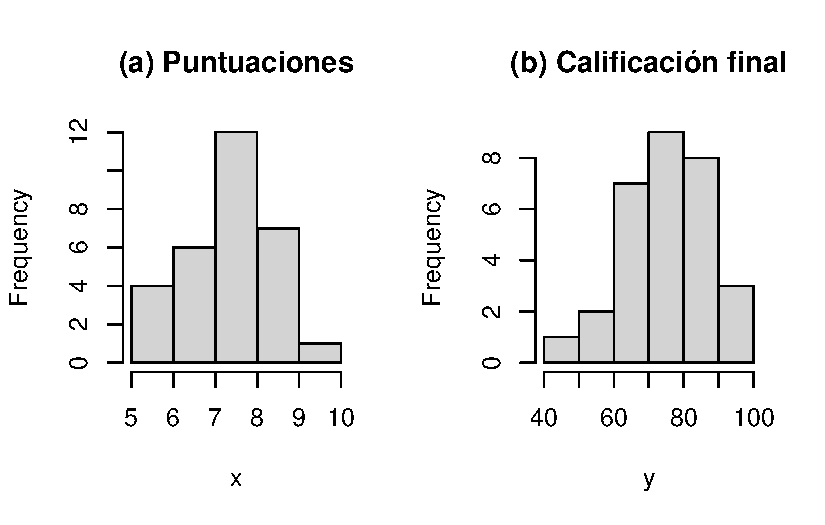
\includegraphics{estadistica_files/figure-pdf/unnamed-chunk-2-1.pdf}

}

\caption{\label{fig-histo}Puntajes y calificaciones finales para una
muestra aleatoria de 30 estudiantes inscritos al curso.}

\end{figure}%

\end{tcolorbox}

Los histogramas, las medias y las desviaciones estándar no proporcionan
información sobre cómo dos variables están relacionadas entre sí. Como
ejemplo, un instructor probablemente quisiera saber si los estudiantes
que les fue bien en el cuestionario también tendieron a desempeñarse
bien en el examen final, y viceversa. También podría querer saber si
algunos estudiantes que les fue mal en el cuestionario mejoraron
drásticamente su calificación en el examen final. Los histogramas y las
estadísticas de muestra mostrados anteriormente no responden a estas
preguntas.

Lo que se necesita son medidas de la relación entre las dos variables.
Los parámetros poblacionales más comunes utilizados para medir tales
relaciones son la covarianza, \(\gamma_{XY}\), y la correlación,
\(\rho_{XY}\).

\begin{definition}[Covarianza]\protect\hypertarget{def-cov}{}\label{def-cov}

Si \(X\) e \(Y\) son dos variables aleatorias definidas en el mismo
espacio de probabilidad, la \emph{covarianza} de \(X\) e \(Y\), denotada
como \(\mathrm{Cov}[X,Y]\) o \(\gamma_{XY}\), se define como
\[\gamma_{XY}=\mathrm{Cov}[X,Y]=\mathrm E[(X-\mu_X)(Y-\mu_Y)]\] siempre
que la esperanza indicada exista.

\end{definition}

\begin{definition}[Correlación]\protect\hypertarget{def-corr}{}\label{def-corr}

La \emph{correlación}, denotada como \(\rho[X,Y]\) o \(\rho_{XY}\), de
las variables aleatorias \(X\) e \(Y\), se define como

\[ \rho_{XY}=\frac{\gamma_{XY}}{\sigma_X \sigma_Y} \]

siempre que \(\gamma_{XY}, \sigma_X\) y \(\sigma_Y\) existan, con
\(\sigma_X, \sigma_Y>0\).

\end{definition}

Técnicamente, la covarianza es el valor esperado (o promedio teórico)
del producto cruzado \((X-\mu_X)(Y-\mu_Y)\). Es una medida de cómo dos
variables ``se mueven juntas''. Para facilitar la interpretación,
generalmente se usa la correlación, que es una versión ``estandarizada''
de la covarianza que tiene la propiedad \(-1 \leq \rho_{XY}\leq 1\) para
cualquier par de variables aleatorias \(X\) e \(Y\).

\begin{remark}
\leavevmode

\begin{enumerate}
\def\labelenumi{\alph{enumi}.}
\item
  \(\gamma_{XX}=\mathrm E[(X-\mu_X)(X-\mu_X)]=\mathrm E[(X-\mu_X)^2]=\sigma_X^2\).
\item
  \(\rho_{XX}=\frac{\sigma_X^2}{\sigma_X \sigma_X}=1\).
\end{enumerate}

\end{remark}

\begin{corollary}[]\protect\hypertarget{cor-covind}{}\label{cor-covind}

Si \(X\) e \(Y\) son independientes, entonces \(\gamma_{XY}=0\).

\begin{proof}
Observe que

\[ \begin{split}\mathrm{Cov}[X,Y]=\mathrm E[(X-\mu_X)(Y-\mu_Y)]=\mathrm E[X-\mu_X]\mathrm E[Y-\mu_Y]=0,\end{split} \]

ya que \(\mathrm E[(X-\mu_X)]=0\).
\end{proof}

\end{corollary}

\begin{theorem}[]\protect\hypertarget{thm-propiedades}{}\label{thm-propiedades}

Sean \(X\) e \(Y\) variables aleatorias definidas sobre el mismo espacio
de probabilidad tales que \(E(X^2) < \infty\) y \(E(Y^2) < \infty\).
Entonces:

\begin{enumerate}
\def\labelenumi{\roman{enumi}.}
\item
  \(\mathrm{Cov}[X, Y]= \mathrm{E}[XY]-\mathrm{E}[X]\mathrm{E}[Y]\).
\item
  \(\mathrm{Cov}[X, Y]= \mathrm{Cov}[Y,X]\).
\item
  \(\mathrm{Var}[X]= \mathrm{Cov}[X,X]\).
\item
  \(\mathrm{Cov}[aX+b, Y]= a\mathrm{Cov}[X, Y]\) para cualquier
  \(a,b \in\mathbb{R}\).
\end{enumerate}

\begin{proof}
Vea Castañeda, Arunachalam, y Dharmaraja (2014).
\end{proof}

\end{theorem}

\begin{definition}[Variables aleatorias no
correlacionadas]\protect\hypertarget{def-uncorr}{}\label{def-uncorr}

Las variables aleatorias \(X\) e \(Y\) se definen como no
correlacionadas si y solo si \(\mathrm{Cov}[X,Y]=0\).

\end{definition}

\begin{remark}
La afirmación contraria al corolario anterior no siempre es cierta; es
decir, \(\mathrm{Cov}[X,Y]=0\) no siempre implica que \(X\) e \(Y\) sean
independientes.
\end{remark}

\chapter{Procesos estocásticos}\label{procesos-estocuxe1sticos}

Los procesos estocásticos desempeñan un papel fundamental en la
modelización y análisis de una amplia gama de fenómenos en diversas
disciplinas, desde la física hasta la economía. Estos procesos son
esenciales para comprender y predecir el comportamiento de sistemas que
involucran aleatoriedad y variabilidad en el tiempo.

Un proceso estocástico (o probabilístico) puede considerarse una
generalización de una muestra aleatoria, en el sentido de que las
variables aleatorias \textbf{no son necesariamente independientes} y su
distrbución podría cambiar. (Castañeda, Arunachalam, y Dharmaraja 2014)
proporciona la siguiente definición para proceso estocástico.

\begin{definition}[Proceso
estocástico]\protect\hypertarget{def-PE}{}\label{def-PE}

Un \emph{proceso estocástico} real es una colección de variables
aleatorias \(\{X_t;\  t\in T\}\) definida en un espacio de probabilidad
común \((\Omega, \mathfrak{F}, P)\) con valores en \(\mathbb{R}\). \(T\)
se le llama al conjunto índice del proceso o espacio paramétrico, que
generalmente es un subconjunto de \(\mathbb R\). El conjunto de valores
que la variable aleatoria \(X_t\) puede tomar se denomina \emph{espacio
de estado del proceso} y es denotado por \(S\).

\end{definition}

De la definición anterior se entiende que las variables
\emph{dependerán} del parámetro \(t\) (usualmente el tiempo) y están
ordenadas. Además, el conjunto \(T\) puede ser discreto o continuo. Si
el conjunto de índices \(T\) es discreto, se le conoce como
\emph{proceso estocástico de tiempo discreto} mientras que si \(T\) es
continuo, se le conoce como \emph{proceso estocástico de tiempo
continuo}. Las variables aleatorias \(X_t\) pueden tomar tanto valores
continuos como valores discretos. Note que si se fija un punto \(t\), se
tiene \(X_t\) una variable aleatoria (Ross 1995).

\begin{definition}[Trayectoria]\protect\hypertarget{def-realiza}{}\label{def-realiza}

La asignación definida para cada \(\omega\in\Omega\) fijo,
\[\begin{split}X(\omega):\ &T\to S\\ &t\mapsto X_t(\omega)\end{split}\]
se denomina una trayectoria de muestra del proceso a lo largo del tiempo
o una realización del proceso estocástico.

\end{definition}

\begin{definition}[Proceso completamente
específicado]\protect\hypertarget{def-pcesp}{}\label{def-pcesp}

Se dice que un proceso estocástico \(\{X(t): t\in T\}\) está
completamente especificado si para cualquier valor del tiempo
\(t_1<t_2<\cdots<t_n\) con \(n\in\mathbb N\), la distribución conjunta
de \((X_{t_1}, X_{t_2},\cdots,X_{t_n})\) es conocida.

\end{definition}

\begin{definition}[Proceso estocástico con incrementos
independientes]\protect\hypertarget{def-incind}{}\label{def-incind}

Si para todo \(t_0,t_1,t_2,\ldots,t_n\) tal que
\(t_0<t_1<t_2<\cdots<t_n\), las variables aleatorias
\(X_{t_0}, X_{t_1}-X_{t_0}, X_{t_2}-X_{t_1},\ldots,X_{t_n}-X_{t_{n-1}}\)
son independientes (o de manera equivalente, \(X_{t+\tau}-X_\tau\) es
independiente de \(X_s\) para \(s< \tau\)), entonces se dice que el
proceso \(\{X_t;\ t\in T\}\) es un \emph{proceso con incrementos
independientes.}

\end{definition}

\begin{remark}
No resulta pertinente afirmar que \(X_{t_1}\) sea inferior a \(X_{t_2}\)
dado que las variables aleatorias no se encuentran ordenadas.
\end{remark}

\begin{definition}[Proceso estocástico con incrementos
estacionarios]\protect\hypertarget{def-incest}{}\label{def-incest}

Se dice que un proceso estocástico \(\{X_t;\ t\in T\}\) tiene
\emph{incrementos estacionarios} si \(X_{t_2+\tau}-X_{t_1+\tau}\) tiene
la misma distribución que \(X_{t_2}-X_{t_1}\) para todas las elecciones
de \(t_1,t_2\) y \(\tau>0\).

\end{definition}

\begin{definition}[Proceso
estacionario]\protect\hypertarget{def-procesoest}{}\label{def-procesoest}

Si para cualquier conjunto de \(t_1, t_2, \ldots , t_n\) arbitrarios,
tal que \(t_1< t_2 < \cdots < t_n\), las distribuciones conjuntas de las
variables aleatorias vectoriales \((X_{t_1}, X_{t_2},\ldots, X_{t_n})\)
y \((X_{t_1+h}, X_{t_2+h},\ldots , X_{t_n+h})\) son iguales para todo
\(h > 0\), entonces se dice que el proceso estocástico
\(\{X_t,\ t \in T\}\) es un proceso estacionario estocástico de orden
\(n\) (o simplemente un \emph{proceso estacionario}). El proceso
estocástico \(\{X_t,\ t \in T\}\) se dice que es un \emph{proceso
estocástico fuertemente estacionario} o e\emph{strictamente
estacionario} si la propiedad anterior se cumple para todo \(n\).

\end{definition}

\begin{tcolorbox}[enhanced jigsaw, breakable, colbacktitle=quarto-callout-caution-color!10!white, rightrule=.15mm, toptitle=1mm, colback=white, left=2mm, colframe=quarto-callout-caution-color-frame, bottomtitle=1mm, opacitybacktitle=0.6, leftrule=.75mm, arc=.35mm, title={Ejemplo}, coltitle=black, titlerule=0mm, opacityback=0, bottomrule=.15mm, toprule=.15mm]

Suponga que \(\{X_n;\ n \geq 1\}\) es una secuencia de variables
aleatorias independientes e idénticamente distribuidas. Se define la
secuencia \(\{Y_n,\ n \geq 1\}\) como

\[
Y_n=X_n+aX_{n-1}
\]

donde \(a\) es una constante real. Entonces, es fácil observar que
\(\{Y_n;\ n \geq 1\}\) es estrictamente estacionaria.

\end{tcolorbox}

\begin{definition}[Proceso de segundo
orden]\protect\hypertarget{def-SOP}{}\label{def-SOP}

Un proceso estocástico \(\{X_t;\ t\in T\}\) se dice un \emph{proceso de
segundo orden} si

\[
\mathrm{E}((X_t)^2)< \infty
\]

para todo \(t\in T\).

\end{definition}

\begin{definition}[Proceso estacionario por
covarianza]\protect\hypertarget{def-PEC}{}\label{def-PEC}

Un proceso estocástico de segundo orden \(\{X_t,\ t \in T\}\) se
denomina \emph{estacionario por covarianza} o \emph{estacionario débil}
si su función de media \(m(t) = \mathrm{E}[X_t]\) es independiente de
\(t\) y su función de covarianza \(\mathrm{Cov}(X_s, X_t)\) depende
únicamente de la diferencia \(|t - s|\) para todos \(s, t \in T\). Es
decir:

\[
\mathrm{Cov}(X_s,X_t)=f(|t-s|).
\]

\end{definition}

\begin{tcolorbox}[enhanced jigsaw, breakable, colbacktitle=quarto-callout-caution-color!10!white, rightrule=.15mm, toptitle=1mm, colback=white, left=2mm, colframe=quarto-callout-caution-color-frame, bottomtitle=1mm, opacitybacktitle=0.6, leftrule=.75mm, arc=.35mm, title={Ejemplo}, coltitle=black, titlerule=0mm, opacityback=0, bottomrule=.15mm, toprule=.15mm]

Sea \(\{X_n;\ n \geq 1\}\) un conjunto de variables aleatorias no
correlacionadas con media cero y varianza uno. Entonces, la covarianza
\(\mathrm{Cov}(X_m, X_n) = \mathrm{E}(X_mX_n)\) es igual a \(0\) si
\(m \ne n\) y \(1\) si \(m = n\). Esto demuestra que
\(\{X_n,\ n \ge 1\}\) es un proceso estacionario por covarianza.

\end{tcolorbox}

\begin{definition}[Proceso
evolutivo]\protect\hypertarget{def-EP}{}\label{def-EP}

Un proceso estocástico que no es estacionario (en ningún sentido), se
dice ser un proceso estocástico evolutivo.

\end{definition}

\part{Series de tiempo}

\chapter{Series de Tiempo}\label{series-de-tiempo-1}

Las series temporales tienen su origen en la necesidad de comprender y
predecir patrones presentes en datos secuenciales en el transcurso del
tiempo. A lo largo de la historia, diversas civilizaciones han
registrado observaciones cronológicas con el propósito de anticipar
fenómenos naturales, eventos económicos y otros procesos cambiantes.

No obstante, el enfoque más sistemático en el análisis de series
temporales se inició en el ámbito de la estadística y la econometría
durante el siglo XX. Figuras pioneras como Norbert Wiener y Andrey
Kolmogorov establecieron los cimientos teóricos en torno a los procesos
estocásticos (Wiener (1949)).

La relevancia de las series temporales en la predicción de datos radica
en su habilidad para capturar patrones temporales y tendencias presentes
en conjuntos de datos. A medida que se acumulan datos a lo largo del
tiempo, es posible identificar relaciones y ciclos que facilitan la
realización de pronósticos futuros. Esto resulta especialmente valioso
en campos como la economía, la meteorología, la epidemiología y las
finanzas, donde comprender los patrones temporales es crucial para tomar
decisiones informadas.

En la actualidad, con el advenimiento de la computación y las técnicas
de análisis más avanzadas, las series temporales han adquirido una
importancia aún mayor. Modelos matemáticos y estadísticos avanzados,
como los modelos ARIMA (Media Móvil Integrada Autoregresiva) y las redes
neuronales recurrentes, permiten analizar y predecir series temporales
con mayor precisión y complejidad. Estos modelos son esenciales para la
toma de decisiones estratégicas en diversas industrias, ya que ayudan a
anticipar tendencias, identificar patrones estacionales y enfrentar la
incertidumbre en el futuro.

En términos generales, una serie temporal puede considerarse como una
recopilación de observaciones realizadas secuencialmente en el tiempo.
El interés de este análisis no recae en las series que son
deterministas, sino en aquellas cuyos valores se comportan siguiendo las
leyes de la probabilidad. Se discutirán los principios fundamentales
involucrados en el análisis estadístico de series temporales. Para
comenzar, se debe prestar una atención más meticulosa a la definición de
serie temporal, dado que en realidad es un tipo particular de proceso
estocástico.

\section{Conceptos básicos y manipulación de series de
tiempo}\label{conceptos-buxe1sicos-y-manipulaciuxf3n-de-series-de-tiempo}

\begin{definition}[Serie de
tiempo]\protect\hypertarget{def-ts}{}\label{def-ts}

Un proceso estocástico \(X(t); t\in T\) se define como una colección de
variables aleatorias, donde \(T\) es un conjunto de índices para el cual
todas las variables aleatorias, \(X(t)\), donde \(t\) pertenece a \(T\),
están definidas en el mismo espacio muestral. Cuando \(T\) representa el
tiempo, se hace referencia al proceso estocástico como una \emph{serie
de tiempo}.

\end{definition}

Si \(T\) toma un rango continuo de valores (por ejemplo,
\(T=(-\infty,\infty)\) o \(T=(0,\infty)\)) , el proceso se dice que es
un \emph{proceso de parámetro continuo}. Si, por otro lado, \(T\) toma
un conjunto discreto de valores (por ejemplo, \(T = \{0, 1, 2,\ldots\}\)
o \(T = \{0, \pm 1, \pm 2,\ldots \}\)), el proceso se dice que es un
\emph{proceso de parámetro discreto}. De hecho, es común referirse a
estos como
\hyperref[procesoux5cux2520estocuxe1sticoux5cux2520deux5cux2520tiempoux5cux2520discreto]{procesos
continuos} y
\hyperref[procesoux5cux2520estocuxe1sticoux5cux2520deux5cux2520tiempoux5cux2520continuo]{discretos},
respectivamente.

Se utilizará la notación de subíndice, \(X_t\), cuando se esté tratando
específicamente con un proceso de parámetro discreto. Sin embargo,
cuando el proceso involucrado sea de parámetro continuo o de tipo no
especificado, se utilizará la notación de función, \(X(t)\). Además,
cuando no haya confusión, a menudo se utiliza la notación \(\{X(t)\}\) o
simplemente \(X(t)\) para denotar una serie de tiempo. De manera
similar, a menudo se acortará \(\{X_t;t=0,\pm 1,\ldots \}\) a
\(X_t,t=\{0,\pm 1,\ldots\}\) o simplemente se usará \(X_t\).

Nótese que una variable aleatoria, \(\gamma\) , es una función definida
en un espacio muestral \(\Omega\) cuyo rango son los números reales. Un
valor observado de la variable aleatoria \(\gamma\) es un número real
\(y=\gamma(\omega)\) para algún \(\omega\in\Omega\). Para una serie de
tiempo \(\{X(t)\}\), su ``valor'' \(\{X(t,\omega);t\in T\}\) para algún
\(\omega\in\Omega\) fijo es una colección de números reales. Esto lleva
a la siguiente definición.

\begin{definition}[Realización]\protect\hypertarget{def-realizacion}{}\label{def-realizacion}

Una \emph{realización} de la serie de tiempo \(\{X(t);t\in T\}\) es el
conjunto de resultados de valores reales, \(\{X(t,\omega);t\in T\}\)
para un valor fijo de \(\omega \in \Omega\).

\end{definition}

La colección de todas las posibles realizaciones se denomina
\emph{conjunto} y, para un valor dado de \(t\), la expectativa de la
variable aleatoria \(X(t)\) se denomina \emph{media del conjunto} y se
denotará como \(\mathrm E[X(t)]=\mu(t)\) . La \emph{varianza} de
\(X(t)\) se expresa como

\[
\mathrm{Var}[X(t)]:=\mathrm{E}[(X(t)-\mu(t))^2]
\]

y a menudo se denota como \(\sigma^2(t)\) ya que también puede depender
de \(t\).

\phantomsection\label{.remark}
De especial interés, en el análisis de una serie temporal, es la
covarianza entre \(X(t_1)\) y \(X(t_2)\), donde \(t_1, t_2\in T\). Dado
que esta es la \hyperref[def-cov]{covarianza} dentro de la misma serie
temporal, se refiere a ella como \emph{autocovarianza}. De igual manera,
se refiere a la \hyperref[def-corr]{correlación} dentro de una misma
serie como \emph{autocorrelación} y se denotan por

\begin{equation}\phantomsection\label{eq-autocov}{
\gamma(t_1,t_2):=\mathrm{E}[(X(t_1)-\mu(t_1))(X(t_2)-\mu(t_2))]
}\end{equation}

y

\begin{equation}\phantomsection\label{eq-autocorr}{
\rho(t_1,t_2):= \frac{\gamma(t_1,t_2)}{\sigma(t_1)\sigma(t_2)} 
}\end{equation}

respectivamente.

\subsection{Series de tiempo
estacionarias}\label{series-de-tiempo-estacionarias}

En el estudio de una serie de tiempo, es común que solo se tenga
disponible una única realización de la serie. El análisis de una serie
temporal basado únicamente en una realización es análogo a analizar las
propiedades de una variable aleatoria en función de una sola
observación. Los conceptos de estacionariedad y ergodicidad jugarán un
papel importante en mejorar la capacidad de análisis de una serie
temporal basada en una única realización de manera efectiva. Un proceso
se considera estacionario si está en un estado de ``equilibrio
estadístico''. El comportamiento básico de dicha serie de tiempo no
cambia con el tiempo. Como ejemplo, para dicho proceso, \(\mu(t)\) no
dependería del tiempo y, por lo tanto, podría ser denotado como \(\mu\)
para todo \(t\). Parecería que, dado que \(x(t)\) para cada \(t\in T\),
proporciona información sobre la media del conjunto \(\mu\), podría ser
posible estimar \(\mu\) en función de una única realización. Un proceso
\textbf{ergódico} es aquel para el cual promedios de conjunto como
\(\mu\) pueden estimarse consistentemente a partir de una sola
realización. En esta sección, se presentarán definiciones más formales
de estacionariedad. La noción más restrictiva de estacionariedad es la
de estacionariedad estricta, que se define de la siguiente manera.

\begin{definition}[Proceso estrictamente
estacionario]\protect\hypertarget{def-PPE}{}\label{def-PPE}

Se dice que un proceso \(\{X(t); t \in T\}\) es estrictamente
estacionario si para cualquier \(t_1, t_2,\ldots, t_k \in T\) y
cualquier \(h \in T\), la distribución conjunta de
\(\{X(t_1), X(t_2),\ldots , X(t_k)\}\) es idéntica a la de
\(\{X(t_1 + h), X(t_2 + h),\ldots, X(t_k + h)\}\).

\end{definition}

La estacionariedad estricta requiere, entre otras cosas, que para
cualquier \(t_1, t_2 \in T\), las distribuciones de \(X(t_1)\) y
\(X(t_2)\) deben ser las mismas, y además que todas las distribuciones
bivariadas de pares \(\{X(t), X(t + h)\}\) sean iguales para todos los
\(h\), etc. El requisito de estacionariedad estricta es riguroso y suele
ser difícil de establecer matemáticamente. De hecho, para la mayoría de
las aplicaciones, las distribuciones involucradas no se conocen. Por
esta razón, se han desarrollado nociones menos restrictivas de
estacionariedad. La más común de ellas es la estacionariedad por
covarianza.

\begin{definition}[Estacionariedad por
covarianza]\protect\hypertarget{def-estcov}{}\label{def-estcov}

La serie de tiempo \(\{X(t); t \in T\}\) se considera estacionaria por
covarianza si

\begin{enumerate}
\def\labelenumi{\roman{enumi}.}
\item
  \(\mu_{_{X_t}}=\mathrm E[X(t)] = \mu\) (media constante para todo
  \(t\)).
\item
  \(\sigma^2_{_{X_t}}=\mathrm{Var}[X(t)] = \sigma^2 < \infty\) (es
  decir, una constante finita para todo \(t\)).
\item
  \(\gamma_{_{X_{t_1},X_{t_2}}}\) y \(\rho_{_{X_{t_1},X_{t_2}}}\)
  depende solo de \(t_2 − t_1\).
\end{enumerate}

\end{definition}

Si se cumple la condición iii., no habrá confusión al reemplazar la
notación \(\gamma_{_{X_{t_1},X_{t_2}}}\) con \(\gamma_{_{t_1-t_2}}\) y,
de manera similar, al denotar \(\rho_{_{X_{t_1},X_{t_2}}}\) como
\(\rho_{_{t_1-t_2}}\). Cuando se establece \(t_2-t_1=k\), se hace
referencia a \(\gamma_{_k}\) y \(\rho_{_k}\) como la autocovarianza y la
autocorrelación con un rezago de \(k\), respectivamente.

La función de autocovarianza de una serie de tiempo estacionaria
satisface las siguientes propiedades:

\begin{enumerate}
\def\labelenumi{\roman{enumi}.}
\item
  \(\gamma_{_0}=\mathrm E[(X_{t}-\mu)(X_{t}-\mu)]=\mathrm E[(X_{t}-\mu)^2]=\sigma^2\).
\item
  \(|\gamma_{_k}|\leq \gamma_{_0}\) para todo \(k\).
\item
  \(\gamma_{_k}=\mathrm{E}[(X_{t-k}-\mu)(X_t-\mu)]=\mathrm{E}[(X_t-\mu)(X_{t-k}-\mu)]=\gamma_{_{-k}}\).
\item
  La función \(\gamma_{_k}\) es semidefinida positiva. Esto es, para
  cualquier conjunto de puntos de tiempo \(t_1, t_2,\ldots,t_k\in T\) y
  para los reales \(b_1,b_2,\ldots, b_k\), se tiene

  \[\sum_{i=1}^k \sum_{j=1}^k \gamma(t_i-t_j)b_i b_j\geq 0.
  \]
\end{enumerate}

La función de autocorrelación satisface las siguientes propiedades
análogas:

\begin{enumerate}
\def\labelenumi{\roman{enumi}.}
\item
  \(\rho_{_0} = 1\).
\item
  \(|\rho_{_k}|\leq 1\) para todo \(k\).
\item
  \(\rho_{_k}=\rho_{_{-k}}\).
\item
  La función \(\rho_{_k}\) es semidefinida positiva, y para series de
  tiempo discretas definidas en \(t = 0, 1, 2,\ldots\), la matriz

  \[
  \boldsymbol{\rho}_k = \begin{pmatrix}1 & \rho_1 & \ldots & \rho_{_k}\\
  \rho_1 & 1 & \ldots & \rho_{k-1}\\
  \vdots & \vdots & \ddots & \vdots\\
  \rho_{_k} & \rho_{k+1}&\ldots & 1\end{pmatrix}
  \]

  es semidefinida positiva para cada \(k\).
\end{enumerate}

\begin{remark}
La estacionariedad por covarianza también se conoce como estacionariedad
débil, estacionariedad en el sentido amplio y estacionariedad de segundo
orden. En el resto de esta tesis, a menos que se especifique lo
contrario, el término estacionariedad se referirá a la estacionariedad
por covarianza.
\end{remark}

En las series de tiempo, al igual que en la mayoría de las otras áreas
de la estadística, los datos no correlacionados desempeñan un papel
importante. No hay dificultad en definir dicho proceso en el caso de una
serie temporal de parámetro discreto. Es decir, la serie temporal
\(\{X_t; t = 0, \pm 1, \pm 2,\ldots\}\) se llama ``proceso puramente
aleatorio'' si los \(X_t\) son variables aleatorias no correlacionadas.
Al considerar procesos puramente aleatorios, solo nos interesará el caso
en el que los \(X_t\) también estén distribuidos de manera idéntica. En
esta situación, es más común referirse a la serie de tiempo como ruido
blanco. La siguiente definición resume estas observaciones.

\begin{definition}[Proceso de ruido
blanco]\protect\hypertarget{def-ruidob}{}\label{def-ruidob}

Se dice que un proceso \(X_t\) es ruido blanco si se cumplen las
siguientes condiciones.

\begin{enumerate}
\def\labelenumi{\arabic{enumi}.}
\item
  Los \(X_t\) están distribuidos de manera idéntica.
\item
  \(\gamma_{_{t_2-t_1}} = 0\) cuando \(t_2 \ne t_1\).
\item
  \(\gamma_{_{t-t}} = \sigma^2\), donde \(0 < \sigma^2 < \infty\) .
\end{enumerate}

\end{definition}

En un proceso de ruido blanco, cada observación está no correlacionada
con todas las demás observaciones. Un hecho importante es que los
procesos de ruido blanco son estacionarios.

\subsubsection{Estimación de los parámetros de un proceso
estacionario.}\label{estimaciuxf3n-de-los-paruxe1metros-de-un-proceso-estacionario.}

\paragraph{\texorpdfstring{Estimación de
\(\mu\).}{Estimación de \textbackslash mu.}}\label{estimaciuxf3n-de-mu.}

Dada la realización \(\{x_t, t = 1, 2,\ldots , n\}\) de una serie
temporal estacionaria, la estimación natural de la media común \(\mu\)
es la media muestral

\begin{equation}\phantomsection\label{eq-media}{
\bar{x}=\frac{1}{n}\sum_{t=1}^n x_t.
}\end{equation}

Es evidente que el estimador \(\bar{X}\) es imparcial para \(\mu\).

Para una serie temporal estacionaria, se pueden emplear los datos a lo
largo del tiempo para estimar la media, dado que se asume que la media
es constante para cada instante de tiempo \(t\).

\subparagraph{\texorpdfstring{Ergodicidad de
\(X\).}{Ergodicidad de X.}}\label{ergodicidad-de-x.}

Se dice que \(X\) es ergódico para \(\mu\) si \(X\) converge en el
sentido de la media cuadrática hacia \(\mu\) a medida que \(n\) aumenta,
es decir, si \(\lim\limits_{n\to\infty}\mathrm{E}[(\bar X -\mu)^2]=0\).

\begin{theorem}[]\protect\hypertarget{thm-ergo}{}\label{thm-ergo}

Sea \(\{X_t; t=0,\pm 1,\pm 2, \ldots\}\) una serie de tiempo
estacionaria. Entonces, \(\bar X = \frac{1}{n}\sum\limits_{t=1}^n X_t\)
es ergódica para \(\mu\) si y solo si

\begin{equation}\phantomsection\label{eq-ergo}{
\lim\limits_{k\to \infty} \frac{1}{k} \sum_{j=0}^{k-1} \gamma_j =0.
}\end{equation}

\begin{proof}
Vea Yaglom (1962).
\end{proof}

\end{theorem}

\begin{corollary}[]\protect\hypertarget{cor-ergo}{}\label{cor-ergo}

Sea \(X_t\) una serie de tiempo estacionaria con parámetros discretos,
como se establece en el Teorema~\ref{thm-ergo} . Entonces, \(\bar X\) es
ergódico para \(\mu\) si

\begin{equation}\phantomsection\label{eq-ergo1}{
\lim\limits_{k\to\infty} \gamma_{_k}=0,
}\end{equation}

o equivalentemente si

\begin{equation}\phantomsection\label{eq-ergo2}{
\lim\limits_{k\to\infty} \rho_{_k}=0.
}\end{equation}

\end{corollary}

La condición suficiente para la ergodicidad de \(\bar X\), dada en el
Corolario~\ref{cor-ergo}, resulta muy útil y es una condición que se
cumple para la amplia clase de series temporales autorregresivas de
media móvil, ARMA\((p,q)\), estacionarias, que se discutirán más
adelante. A pesar de que \(X_t\)'s ``cercanos'' en el tiempo pueden
tener una correlación sustancial, la condición en el
Corolario~\ref{cor-ergo} asegura que, para una ``gran'' separación,
están casi no correlacionados.

\subparagraph{\texorpdfstring{Varianza de
\(\bar X\).}{Varianza de \textbackslash bar X.}}\label{varianza-de-bar-x.}

Antes de abandonar el tema de estimar \(\mu\) a partir de una
realización de un proceso estacionario, en el Teorema~\ref{thm-varmedia}
se proporciona una fórmula útil para la Varianza de \(\bar X\).

\begin{theorem}[]\protect\hypertarget{thm-varmedia}{}\label{thm-varmedia}

Sea \(X_t\) una serie de tiempo estacionaria, la varianza de \(\bar X\)
basada en una realización de longitud \(n\) está dada por

\begin{equation}\phantomsection\label{eq-varmedia}{
\mathrm{Var}(\bar X)=\frac{\sigma_X^2}{n}\left(1+2\sum_{k=1}^{n-1}\left(1-\frac{|k|}{n}\right)\rho_{_k}\right).
}\end{equation}

\end{theorem}

El resultado en la ecuación (\ref{eq-varmedia}) muestra el efecto de la
autocorrelación en la varianza de \(\bar X\), y si \(X_t\) es ruido
blanco, es decir, \(\gamma_{_{k}} = 0\) si \(k \ne 0\), entonces la
ecuación (\ref{eq-varmedia}) se convierte en el conocido resultado
\(Var(\bar X) = \sigma^2/n\).

Utilizando la notación \(\hat \rho_{_k}\) para denotar las
autocorrelaciones estimadas (muestra) y \(\hat\sigma^2=\hat{\gamma_0}\)
para denotar la varianza muestral, es práctica común obtener intervalos
de confianza aproximados del \(95\%\) para \(\mu\) usando

\begin{equation}\phantomsection\label{eq-iconf}{
\left(\bar X- 1.96\sqrt{\frac{\hat\sigma^2}{n}\sum_{k=-(n-1)}^{n-1}\left(1-\frac{|k|}{n}\right)\hat\rho_{_k}}, \bar X+ 1.96\sqrt{\frac{\hat\sigma^2}{n}\sum_{k=-(n-1)}^{n-1}\left(1-\frac{|k|}{n}\right)\hat\rho_{_k}}\right).
}\end{equation}

\paragraph{\texorpdfstring{Estimación de
\(\gamma_{_k}\).}{Estimación de \textbackslash gamma\_\{\_k\}.}}\label{estimaciuxf3n-de-gamma__k.}

Debido a la estacionariedad,
\(\mathrm E[(X_t − \mu)(X_{t+k} − \mu)] = \gamma_{_k}\) no depende de
\(t.\) Como consecuencia, parece razonable estimar \(\gamma_{_k}\) a
partir de una sola realización, esto es

\begin{equation}\phantomsection\label{eq-estgamma}{
\begin{split}\hat{\gamma}_{_k}&= \frac{1}{n}\sum_{t=1}^{n-k}(X_t-\bar X)(X_{t+k}-\bar X), \quad 0\leq k\leq n\\
&=0,\qquad k\ge n\\
&=\hat{\gamma}_{_{-k}},\quad k<0.\end{split}
}\end{equation}

\begin{remark}
Usando la ecuación (\ref{eq-estgamma}) se deduce que

\begin{equation}\phantomsection\label{eq-hatgamma0}{
\hat{\gamma}_{_0}= \frac{1}{n}\sum_{t=1}^{n}(X_t-\bar X)^2.
}\end{equation}
\end{remark}

\paragraph{\texorpdfstring{Estimación de
\(\rho_{_k}\).}{Estimación de \textbackslash rho\_\{\_k\}.}}\label{estimaciuxf3n-de-rho__k.}

\begin{definition}[Autocorrelación
muestral]\protect\hypertarget{def-samplecorr}{}\label{def-samplecorr}

El estimador de la autocorrelación, \(\rho_{_{k}}\) se obtiene mediante

\begin{equation}\phantomsection\label{eq-sampleautocor}{
\hat\rho_{_{k}}=\hat\gamma_{_{k}}/\hat\gamma_{_{0}}.
}\end{equation}

A este estimador se le conoce como la autocorrelación muestral.

\end{definition}

A partir del análisis de la ecuación (\ref{eq-estgamma}) , es evidente
que los valores de \(\hat\gamma_{_{k}}\) (y \(\hat\rho_{_{k}}\))
tenderán a ser ``pequeños'' cuando \(k\) sea grande en relación con
\(n\).

\subsection{Conjuntos de datos de series
temporales.}\label{conjuntos-de-datos-de-series-temporales.}

Los comportamientos exhibidos por los datos de series temporales son
diversos y se analizarán en las secciones subsiguientes. Dichos tipos de
comportamiento se ilustrarán mediante ejemplos provenientes de la
realidad, tales como los datos intrigantes de manchas solares, registros
de temperatura, el índice Dow Jones, precios de acciones individuales,
datos de ventas (tanto mensuales como diarios), entre otros. El análisis
comenzará con una discusión sobre datos que presenten algún tipo de
patrón cíclico (Woodward, Sadler, y Robertson (2022)).

\subsubsection{Datos Cíclicos}\label{datos-cuxedclicos}

Muchos conjuntos de datos de series temporales muestran un patrón
cíclico, lo que significa que los datos presentan aumentos y
disminuciones de manera algo repetitiva. Estos datos a veces se
denominan \emph{``pseudo-periódicos''}, un término que usaremos de
manera sinónima con \emph{``cíclico''}. Los datos de manchas solares en
la Figura~\ref{fig-sunspot} son un ejemplo de datos cíclicos.

\begin{remark}
Los datos verdaderamente periódicos exhiben un comportamiento que se
replica de manera precisa a lo largo de un período de tiempo
establecido. Un caso ilustrativo de datos puramente periódicos se
encuentra en la forma de la curva sinusoidal. De este modo, los datos
pseudoperiódicos (o cíclicos) se refieren a aquellos conjuntos de datos
que tienden a mostrar repeticiones en sus comportamientos.
\end{remark}

\begin{example}[]\protect\hypertarget{exm-sunspot}{}\label{exm-sunspot}

~

\begin{tcolorbox}[enhanced jigsaw, breakable, colbacktitle=quarto-callout-caution-color!10!white, rightrule=.15mm, toptitle=1mm, colback=white, left=2mm, colframe=quarto-callout-caution-color-frame, bottomtitle=1mm, opacitybacktitle=0.6, leftrule=.75mm, arc=.35mm, title={Datos de manchas solares}, coltitle=black, titlerule=0mm, opacityback=0, bottomrule=.15mm, toprule=.15mm]

La Figura~\ref{fig-sunspot} muestra datos anuales de manchas solares
para los años 1700-2020. Las manchas solares son áreas de explosiones
solares o disturbios atmosféricos extremos en el sol. En 1848, el
astrónomo suizo Rudolf Wolf introdujo un método para contar la actividad
de las manchas solares, y los datos mensuales utilizando su método están
disponibles desde 1749. (Waldmeier (1961)).

\begin{figure}[H]

\centering{

\begin{Shaded}
\begin{Highlighting}[]
\FunctionTok{library}\NormalTok{(tswge)}
\FunctionTok{plot}\NormalTok{(sunspot2}\FloatTok{.0}\NormalTok{, }\AttributeTok{xlab=}\StringTok{\textquotesingle{}Año\textquotesingle{}}\NormalTok{, }\AttributeTok{ylab=}\StringTok{\textquotesingle{}Manchas solares\textquotesingle{}}\NormalTok{)}
\end{Highlighting}
\end{Shaded}

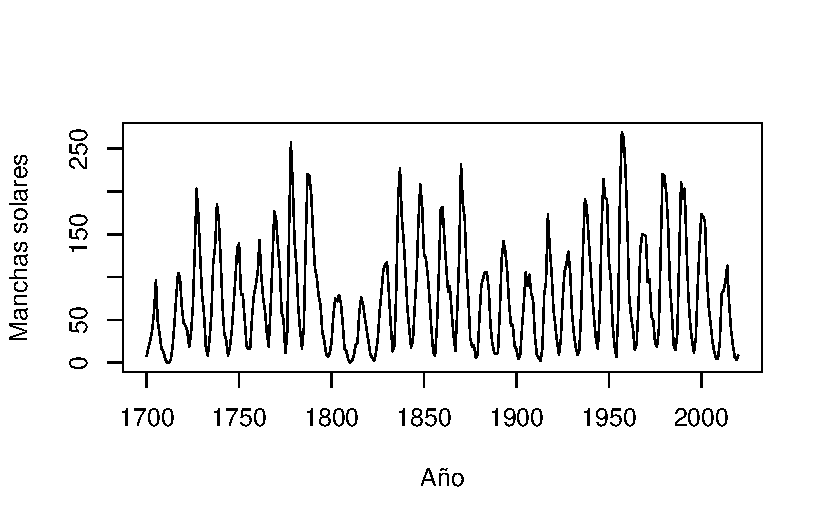
\includegraphics{series_files/figure-pdf/unnamed-chunk-1-1.pdf}

}

\caption{\label{fig-sunspot}Número anual de manchas solares desde 1700
hasta 2020.}

\end{figure}%

Las manchas solares han generado un considerable interés en la comunidad
científica por dos razones principales:

\begin{itemize}
\item
  La actividad de las manchas solares tiende a afectarnos aquí en la
  Tierra. Por ejemplo, una alta actividad de manchas solares provoca
  interferencias en la comunicación por radio y se asocia con una mayor
  intensidad de luz ultravioleta y actividad de auroras boreales.
\item
  La actividad de las manchas solares tiene un comportamiento cíclico
  que tiene una duración de ciclo de aproximadamente 11 años. Al
  examinar la Figura~\ref{fig-sunspot} se observa que hay 29 ciclos en
  los 321 años, con una duración media del ciclo de aproximadamente 11
  años. De hecho, las duraciones de los ciclos tienden a variar
  aleatoriamente entre 9 y 13 años.
\end{itemize}

Si bien, el comportamiento cíclico en la Figura~\ref{fig-sunspot} es
claro, a menudo es útil examinar fragmentos cortos de los datos para
visualizar mejor el comportamiento específico. La
Figura~\ref{fig-sunsfrag} muestra el número de manchas solares desde
1867 hasta 1950. Las líneas verticales identifican los años en los que
hubo un pico en los números de manchas solares y las flechas
horizontales representan el tiempo entre los picos. Para los años
representados en la Figura~\ref{fig-sunsfrag}, las duraciones de los
ciclos fueron de 13, 10, 12, 12, 11, 9 y 10 años, respectivamente. Las
duraciones de los ciclos parecen variar aleatoriamente y no parece haber
un ``ajuste a una duración de ciclo fija''. De hecho, según la
comprensión de estos autores, los científicos no tienen una explicación
física para el ciclo de aproximadamente 11 años. Los datos de las
manchas solares son un ejemplo clásico de datos cíclicos con duraciones
de ciclo variables. De hecho, Yule (1971) desarrolló el proceso
autorregresivo como un medio para describir el comportamiento periódico
``perturbado'' de los datos de las manchas solares.

\begin{figure}[H]

\centering{

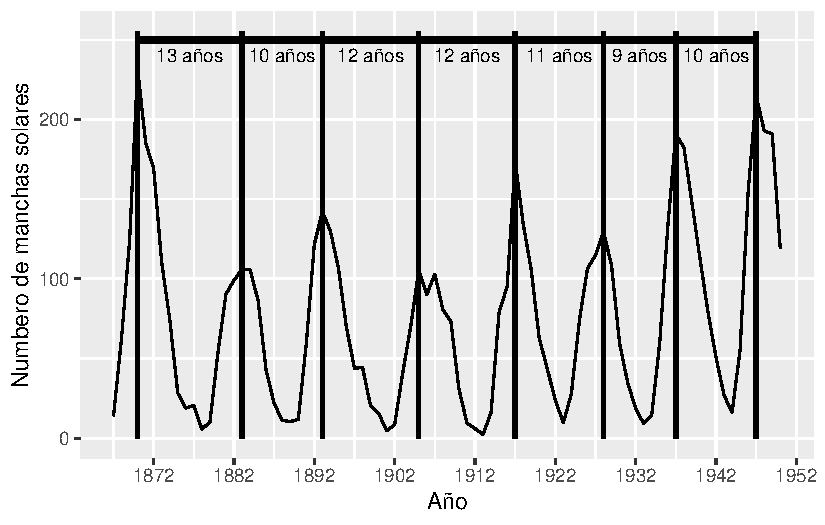
\includegraphics{series_files/figure-pdf/unnamed-chunk-2-1.pdf}

}

\caption{\label{fig-sunsfrag}Fragmento de la Figura~\ref{fig-sunspot}
que muestra los años 1867-1950}

\end{figure}%

\end{tcolorbox}

\end{example}

\begin{example}[]\protect\hypertarget{exm-airpass}{}\label{exm-airpass}

~

\begin{tcolorbox}[enhanced jigsaw, breakable, colbacktitle=quarto-callout-caution-color!10!white, rightrule=.15mm, toptitle=1mm, colback=white, left=2mm, colframe=quarto-callout-caution-color-frame, bottomtitle=1mm, opacitybacktitle=0.6, leftrule=.75mm, arc=.35mm, title={Datos de pasajeros aéreos}, coltitle=black, titlerule=0mm, opacityback=0, bottomrule=.15mm, toprule=.15mm]

La Figura~\ref{fig-airpass} es un conjunto de datos que contiene el
número total (en miles) de pasajeros de líneas aéreas internacionales
por mes durante los 12 años, desde 1949 hasta 1960. Estos datos han sido
analizados exhaustivamente y son un conjunto de datos clásico en la
literatura de series temporales. Los datos siguen un patrón cíclico de
12 meses que es similar de un año a otro y está basado en el año
calendario. Por lo tanto, los datos de pasajeros aéreos son otro ejemplo
de datos estacionales. Además, los datos tienden a mostrar una tendencia
al alza con el tiempo. Es decir, el número de pasajeros de líneas aéreas
está aumentando con el tiempo. El comportamiento de tendencia en series
temporales se discutirá en la Sección~\ref{sec-trend}. También hay una
variabilidad creciente dentro del año. Este tipo de comportamiento es
conocido como \emph{estacionalidad multiplicativa}.

\begin{figure}[H]

\centering{

\begin{Shaded}
\begin{Highlighting}[]
\FunctionTok{library}\NormalTok{(tswge)}
\FunctionTok{plot}\NormalTok{(AirPassengers, }\AttributeTok{xlab=}\StringTok{\textquotesingle{}Año\textquotesingle{}}\NormalTok{, }\AttributeTok{ylab=}\StringTok{\textquotesingle{}Número de pasajeros\textquotesingle{}}\NormalTok{)}
\end{Highlighting}
\end{Shaded}

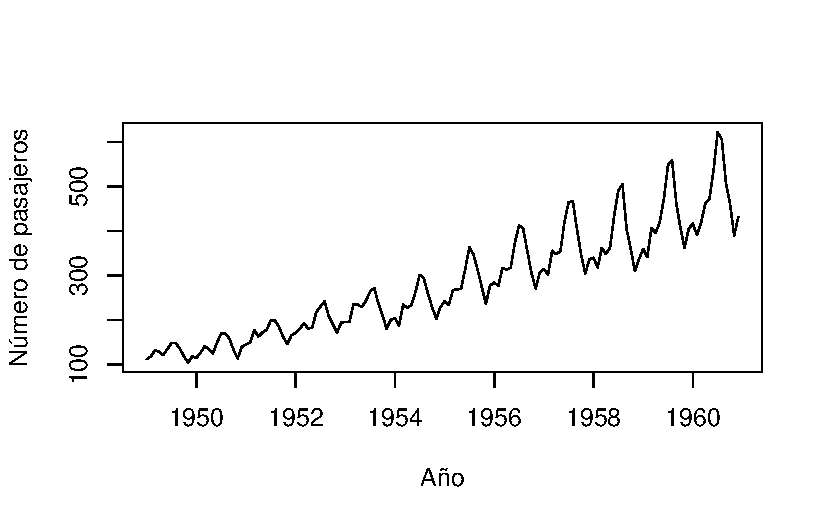
\includegraphics{series_files/figure-pdf/unnamed-chunk-3-1.pdf}

}

\caption{\label{fig-airpass}Número de Pasajeros Internacionales en
Aerolíneas de 1949 a 1960}

\end{figure}%

La Figura~\ref{fig-airfrag} muestra un fragmento de los datos de
pasajeros aéreos desde 1957 hasta 1960. Se observa que el viaje aéreo es
ligero desde Enero hasta Abril, aumenta durante los meses de verano y
comienza a disminuir en septiembre hasta noviembre con un ligero aumento
en diciembre. Este patrón, aunque no es sinusoidal, se repite de un año
a otro. El comportamiento cíclico de los datos de pasajeros aéreos se
repite anualmente y son un ejemplo de datos estacionales que no son
seudosenoidales.

\begin{figure}[H]

\centering{

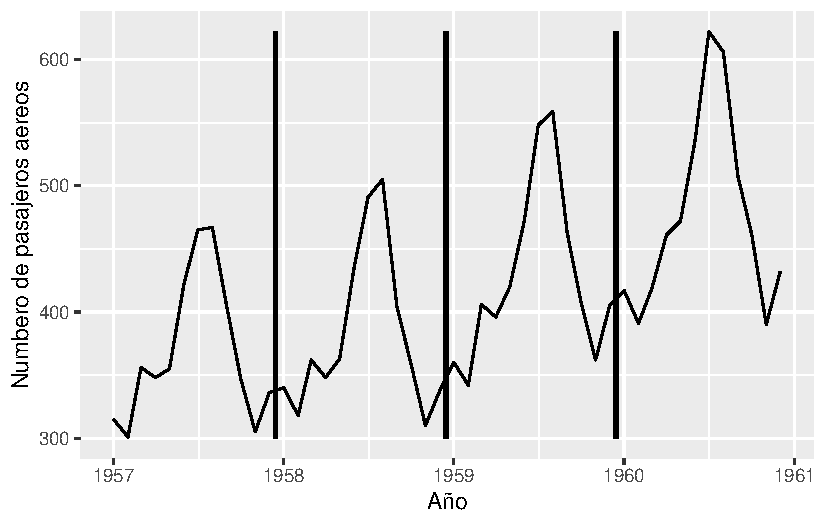
\includegraphics{series_files/figure-pdf/unnamed-chunk-4-1.pdf}

}

\caption{\label{fig-airfrag}Fragmento de la Figura~\ref{fig-airpass} que
muestra los años 1957-1960}

\end{figure}%

\end{tcolorbox}

\end{example}

\subsubsection{Tendencias}\label{sec-trend}

Una tendencia, en un contexto de análisis de datos, se refiere a la
inclinación de una serie de datos al experimentar un incremento o
disminución constante a lo largo del tiempo. En el caso específico de
los datos de Pasajeros Aéreos mostrados en la Figura~\ref{fig-airpass},
se identifica un patrón de crecimiento además del patrón estacional
previamente observado. Una tendencia lineal se caracteriza por el
aumento o la disminución de los datos de manera constante y progresiva,
tal como se ilustra en la Figura~\ref{fig-lineal}. Las tendencias pueden
seguir una curva, como lo ejemplifica la tendencia exponencial en la
Figura~\ref{fig-expo}. Por otro lado, la Figura~\ref{fig-desc} exhibe
una serie temporal con una tendencia descendente, pero su naturaleza es
más irregular en comparación con las tendencias representadas en las
Figuras (a) y (b). Un patrón común en conjuntos de datos es un
comportamiento de tendencia aleatoria, como se muestra en la
Figura~\ref{fig-deam}, la cual sugiere una trayectoria sin un rumbo
definido. Esto implica que pueden existir tendencias de corta o larga
duración, en ocasiones en direcciones opuestas.

\begin{figure}

\begin{minipage}{0.50\linewidth}

\centering{

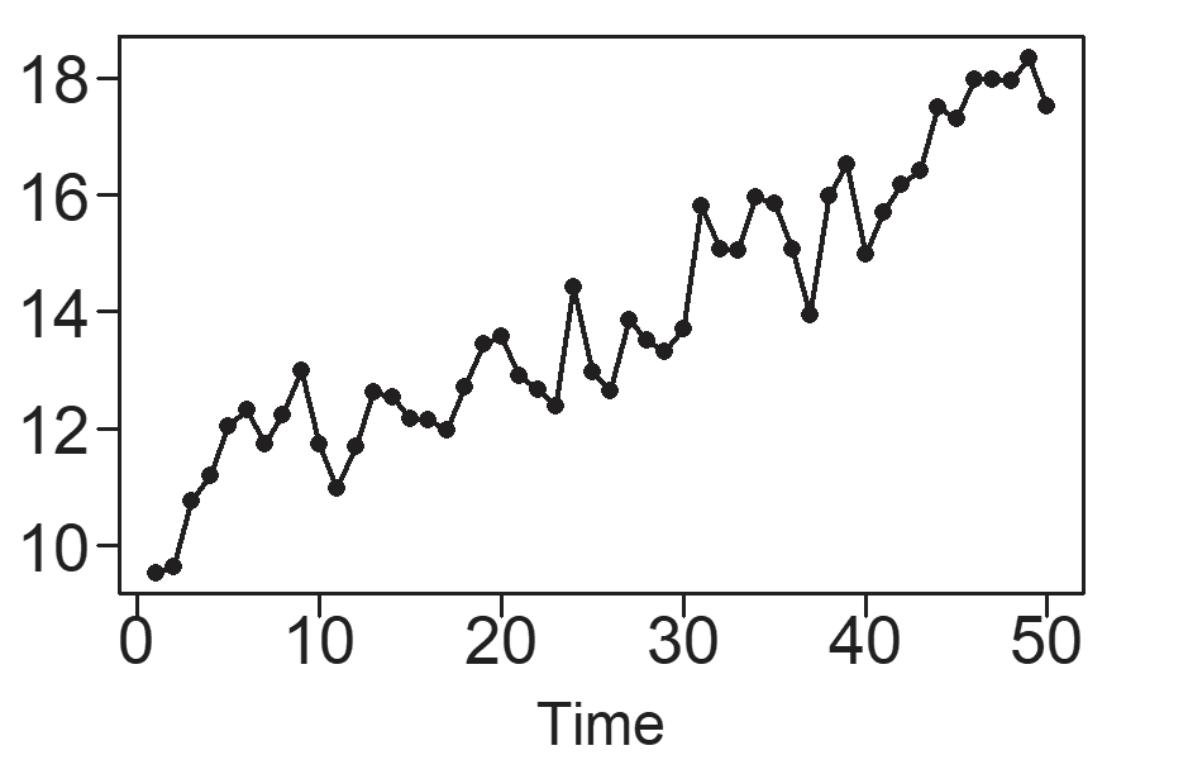
\includegraphics{Imagenes/lineal.png}

}

\subcaption{\label{fig-lineal}Tendencia lineal}

\end{minipage}%
%
\begin{minipage}{0.50\linewidth}

\centering{

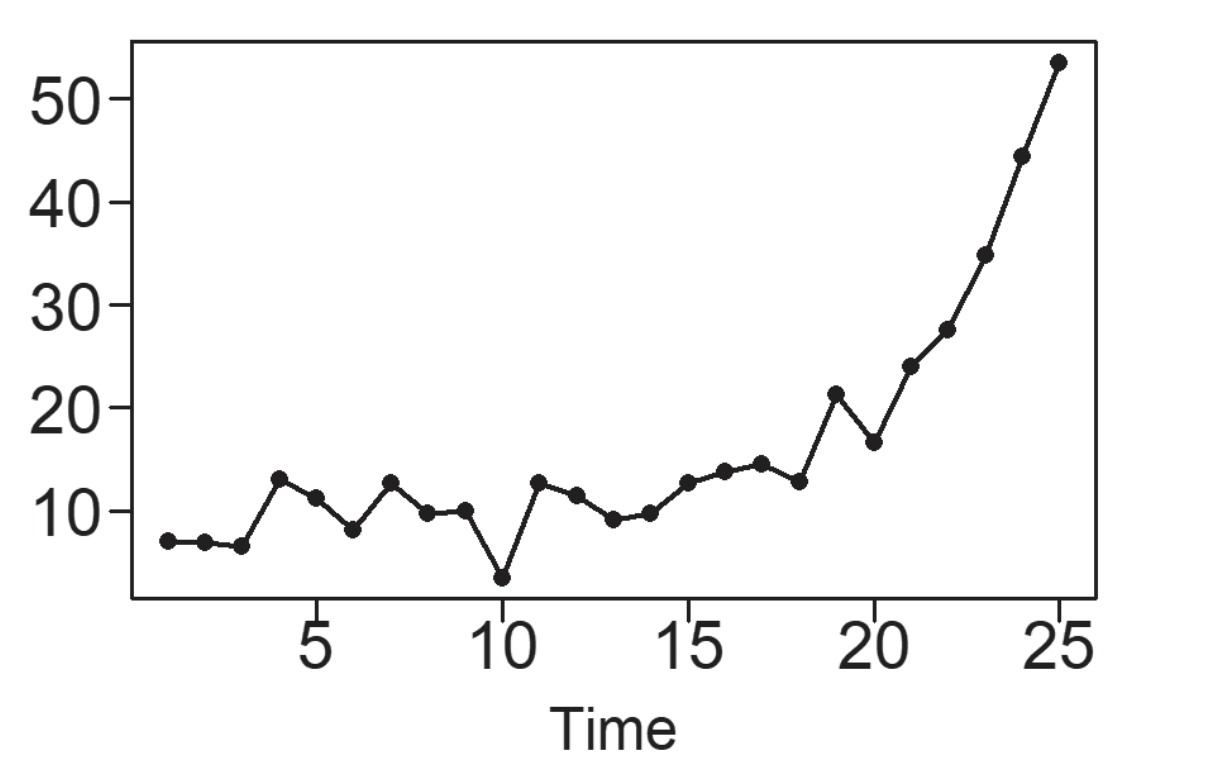
\includegraphics{Imagenes/exponencial.png}

}

\subcaption{\label{fig-expo}Tendencia exponencial}

\end{minipage}%
\newline
\begin{minipage}{0.50\linewidth}

\centering{

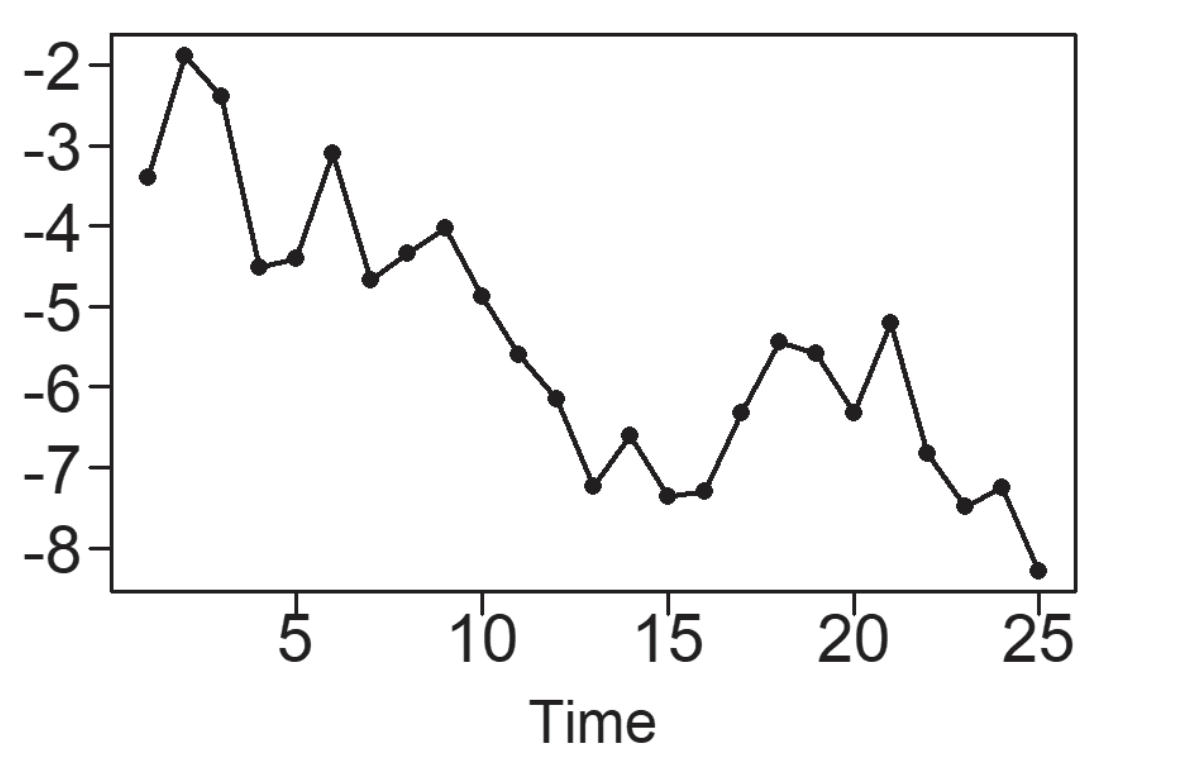
\includegraphics{Imagenes/abajo.png}

}

\subcaption{\label{fig-desc}Tendencia descendente}

\end{minipage}%
%
\begin{minipage}{0.50\linewidth}

\centering{

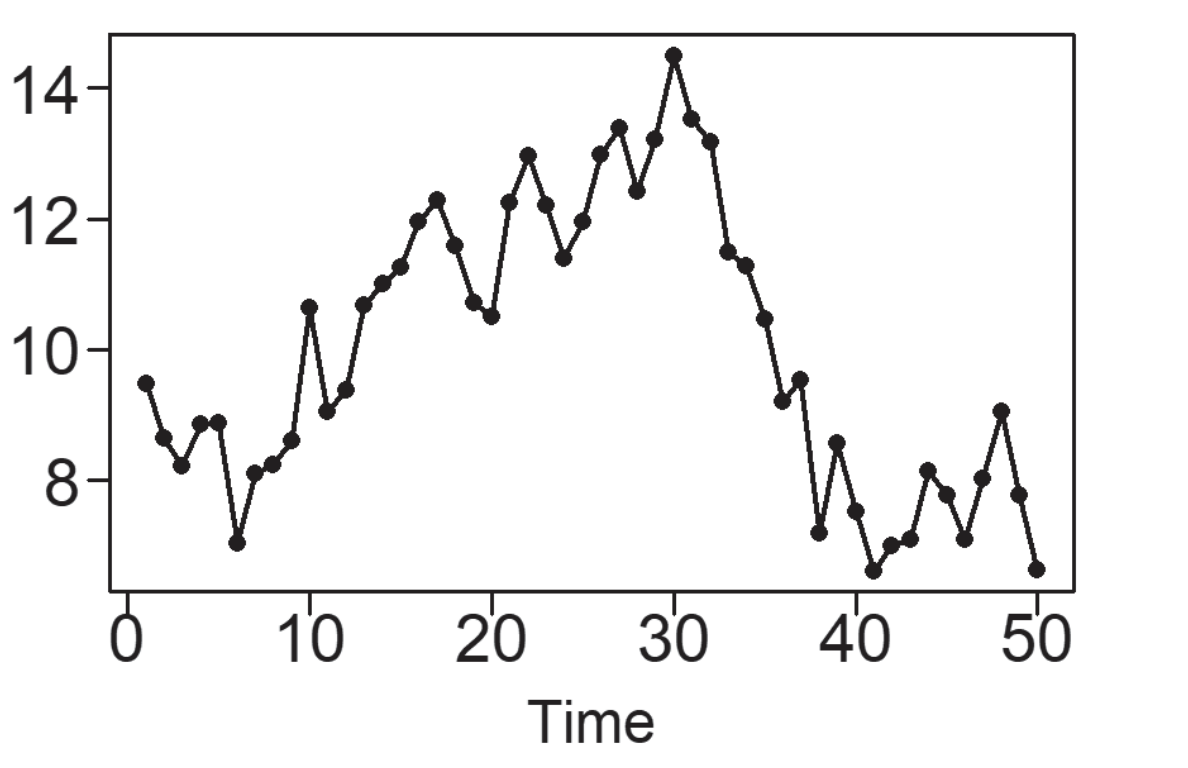
\includegraphics{Imagenes/deambulante.png}

}

\subcaption{\label{fig-deam}Comportamiento deambulante}

\end{minipage}%

\caption{\label{fig-trends}Gráficos que muestran (a) una tendencia
lineal, (b) una tendencia exponencial, (c) una tendencia descendente
irregular y (d) un patrón de deambulación.}

\end{figure}%

\begin{definition}[]\protect\hypertarget{def-aper}{}\label{def-aper}

La función \(g(t)\) es \emph{periódica} con periodo (o longitud del
ciclo) \(p > 0\) si \(p\) es el valor más pequeño tal que
\(g(t) = g(t + kp)\) para todo \(t\) y enteros \(k\). Se dice que una
función \(g(t)\) es \emph{aperiódica} si no existe tal \(p\).

\end{definition}

\begin{definition}[Frecuencia]\protect\hypertarget{def-freq}{}\label{def-freq}

La frecuencia, denotada por \(f\), puede ser descrita de las siguientes
dos maneras;

\begin{enumerate}
\def\labelenumi{\arabic{enumi}.}
\item
  \(f=1/\text{periodo}\) (tamaño del ciclo).
\item
  El número de ciclos en la función a través de una unidad de tiempo.
\end{enumerate}

\end{definition}

\begin{remark}
Los datos con comportamiento de tendencia y deambulación aleatoria no
son cíclicos por naturaleza. A veces se les llama aperiódicos debido a
la ausencia de un comportamiento regular de ascenso y descenso.
\end{remark}

\subsubsection{Definición y propiedades del espectro y densidad
espectral}\label{definiciuxf3n-y-propiedades-del-espectro-y-densidad-espectral}

\begin{definition}[]\protect\hypertarget{def-spec}{}\label{def-spec}

Sea \(X_{_t}\) una serie de tiempo estacionaria con autocovarianza
\(\gamma_{_k}\) y autocorrelación \(\rho_{_k}\). Entonces para
\(|f|\le 0.5\):

\begin{enumerate}
\def\labelenumi{\roman{enumi}.}
\item
  El \emph{espectro} de \(X_{_t}\) se define como

  \begin{equation}\phantomsection\label{eq-spectrum}{
  P_{_X}(f)=\sum_{k=-\infty}^\infty e^{-2\pi ifk}\gamma_{_k}.
  }\end{equation}
\item
  La \emph{densidad espectral} de \(X_{_t}\) se define como

  \begin{equation}\phantomsection\label{eq-spectden}{
  S_{_X}(f)=\sum_{k=-\infty}^\infty e^{-2\pi ifk}\rho_{_k}.
  }\end{equation}
\end{enumerate}

\end{definition}

Usando la fórmula de Euler en las ecuaciones (\ref{eq-spectrum}) y
(\ref{eq-spectden}), se obtienen las siguientes fórmulas.

\[
P_{_X}(f)=\sigma_{_X}^2+2\sum_{k=1}^\infty\gamma_{_k}\cos(2\pi fk),
\]

\[
S_{_X}(f)=1+2\sum_{k=1}^\infty \rho_{_k}\cos(2\pi fk).
\]

Estas fórmulas enfatizan que el espectro y la densidad espectral son
funciones de valor real, lo que no es evidente en las ecuaciones
(\ref{eq-spectrum}) y (\ref{eq-spectden}).

\textbf{\emph{Propiedades importantes de densidades espectrales}}

\begin{enumerate}
\def\labelenumi{\roman{enumi}.}
\item
  \(S_{_X}(f)\geq 0\).
\item
  \(S_{_X}(f)=S_{_X}(-f)\).
\item
  \(S_{_X}(f)=1+2\sum\limits_{k=1}^\infty \rho_{_k}\cos(2\pi fk)\),
  donde \(|f|\le 0.5\) .
\item
  \(\sum\limits_{-0.5}^{0.5}S_{_X}(f)e^{2\pi ifk}df=\rho_{_k}\).

  Las propiedades i y ii muestran que \(S_{_X}(f)\) es una función par
  no negativa.
\end{enumerate}

\subsection{Suavizado de datos de series
temporales.}\label{suavizado-de-datos-de-series-temporales.}

Existen varios métodos para ``suavizar'' el comportamiento ruidoso
(posiblemente poco importante) de una serie temporal, para que se pueda
entender mejor una señal importante subyacente. Se comienza discutiendo
el método de suavizado de promedio móvil centrado, que es el más básico.

\subsubsection{Suavizado de datos utilizando un suavizador de promedio
móvil centrado}\label{sec-mas}

El suavizador de promedio móvil centrado es un método para reemplazar
los valores de datos en una serie temporal con un promedio de los
valores de datos que rodean (e incluyen) ese punto de datos. Por
ejemplo, un suavizador de promedio móvil centrado de orden tres
reemplaza un valor de datos \(x_{_t}\) en el tiempo \(t\) con
\(s_{_t} = (x_{_{t-1}}+x_{_t}+x_{_{t+1}})/3\). Es decir, se asigna el
valor promedio al punto de tiempo medio. Por lo tanto, un suavizador de
promedio móvil centrado de orden tres no puede asignarse al primer o
último punto de tiempo de una serie temporal. Se sigue que a mayor
orden, más valores faltarán al principio y al final del conjunto de
datos suavizado. Para un promedio móvil centrado de tercer orden, la
fórmula de promediado se desplaza a lo largo del conjunto de datos de la
serie temporal, considerando tres valores de datos consecutivos juntos
hasta llegar a los últimos tres puntos temporales.

\begin{definition}[Suavizador de Promedio Móvil
Centrado]\protect\hypertarget{def-CMAS}{}\label{def-CMAS}

Sea \(x_{_t}, t=1,\ldots,n\) un conjunto de datos de series temporales.
El suavizador de promedio móvil centrado se define de la siguiente
manera:

\textbf{\emph{Caso 1:}} \(m\) \textbf{\emph{es un número impar.}}

Sea \(k= (m−1)/2\). Para \(k <t< n - k\), el valor de los datos
suavizados, \(s_{_t}\), en el tiempo \(t\) se da por

\begin{equation}\phantomsection\label{eq-mimpar}{
s_{_t}=\frac{1}{m}\sum_{i=t-k}^{t+k}x_{_i}.
}\end{equation}

\textbf{\emph{Caso 2:}} \(m\) \textbf{\emph{es un número par.}}

Sea \(k= m/2\). Para \(k <t< n - k\), el valor de los datos suavizados,
\(s_{_t}\), en el tiempo \(t\) está dado por

\begin{equation}\phantomsection\label{eq-mpar}{
s_{_t}= \frac{x_{_{t-k}}}{2m}+\frac{1}{m}\sum_{i=t-k+1}^{t+k-1}x_{_i}+\frac{x_{_{t+k}}}{2m}.
}\end{equation}

\end{definition}

\begin{tcolorbox}[enhanced jigsaw, breakable, colbacktitle=quarto-callout-caution-color!10!white, rightrule=.15mm, toptitle=1mm, colback=white, left=2mm, colframe=quarto-callout-caution-color-frame, bottomtitle=1mm, opacitybacktitle=0.6, leftrule=.75mm, arc=.35mm, title={Ejemplos}, coltitle=black, titlerule=0mm, opacityback=0, bottomrule=.15mm, toprule=.15mm]

\begin{itemize}
\item
  Para un promedio móvil centrado de quinto orden en tiempos
  \(2 <t < n -2\) , se tiene

  \[
  s_{_t}=(x_{_{t-2}}+x_{_{t-1}}+x_{_t}+x_{_{t+1}}+x_{_{t+2}})/5.
  \]
\item
  El suavizador de promedio móvil de cuarto orden en tiempos
  \(2 <t < n -2\) , está dado por

  \[
  s_{_t}=\frac{x_{_{t-2}}}{8}+\frac{x_{_{t-1}}+x_{_t}+x_{_{t+1}}}{4}+\frac{x_{_{t+2}}}{8}
  \]
\end{itemize}

El suavizador de promedio móvil centrado tiene dos usos básicos:

\begin{itemize}
\item
  Suavizado diseñado para eliminar fluctuaciones (potencialmente sin
  sentido) de los datos.
\item
  Eliminar el comportamiento cíclico de datos estacionales u otros datos
  cíclicos con longitudes de ciclo fijas.
\end{itemize}

\end{tcolorbox}

El Ejemplo~\ref{exm-ejem} muestra el uso del suavizado de promedio móvil
centrado con el propósito de detectar o comprender mejor señales
subyacentes y fundamentales en los datos.

\begin{example}[]\protect\hypertarget{exm-ejem}{}\label{exm-ejem}

~

\begin{tcolorbox}[enhanced jigsaw, breakable, colbacktitle=quarto-callout-caution-color!10!white, rightrule=.15mm, toptitle=1mm, colback=white, left=2mm, colframe=quarto-callout-caution-color-frame, bottomtitle=1mm, opacitybacktitle=0.6, leftrule=.75mm, arc=.35mm, title={Suavizando los datos de temperatura de Tesla y DFW.}, coltitle=black, titlerule=0mm, opacityback=0, bottomrule=.15mm, toprule=.15mm]

Los precios de las acciones de Tesla desde el 1 de enero de 2020 hasta
el 30 de abril de 2021 se muestran en la Figura~\ref{fig-charts-1}. Se
observa el hecho de que hubo un aumento constante hasta principios de
2021, momento en el cual el precio se estabilizó y disminuyó. Sin
embargo, hay una considerable fluctuación de un día para otro,
especialmente en 2021. La Figura~\ref{fig-charts-4} muestra las
temperaturas medias anuales de DFW (Dallas Ft. Worth) desde 1900 hasta
2020. Allí se observa una considerable fluctuación de un año a otro,
pero algo de aumento a partir de aproximadamente 2000. En la
Figura~\ref{fig-charts}, incisos \ref{fig-charts-2}, \ref{fig-charts-3},
\ref{fig-charts-5} y \ref{fig-charts-6}, se muestran versiones
suavizadas de la misma figura pero de los incisos \ref{fig-charts-1} y
\ref{fig-charts-4}. Al utilizar el suavizador de promedio móvil
centrado, las fluctuaciones de un día para otro se suavizan; se nota que
el orden 8 produce más suavizado que el orden 3. El comportamiento
fundamental, incluida la estabilización y disminución a principios de
2021, se ve con más claridad al minimizar los cambios ruidosos de un día
para otro. El efecto del suavizado es más evidente en los datos de
temperatura de DFW. La fluctuación de un año a otro es bastante
dramática en el conjunto de datos original en la
Figura~\ref{fig-charts-4}. Un suavizado de orden 3 proporciona cierta
claridad, pero el suavizado de orden 8 mostrado en la
Figura~\ref{fig-charts-5} muestra claramente un comportamiento casi
estable desde 1900 hasta aproximadamente 1985. Desde entonces, ha habido
un aumento que puede haberse estabilizado o no en los últimos años. Es
particularmente notable en la Figura~\ref{fig-charts-5} que el suavizado
ha eliminado los extremos. Específicamente, las temperaturas
extremadamente altas en 2012, 2016 y 2017 se ven moderadas por las
temperaturas más bajas en los años circundantes. (Tomado de Woodward,
Sadler, y Robertson (2022))

\begin{figure}[H]

\begin{minipage}{0.33\linewidth}

\centering{

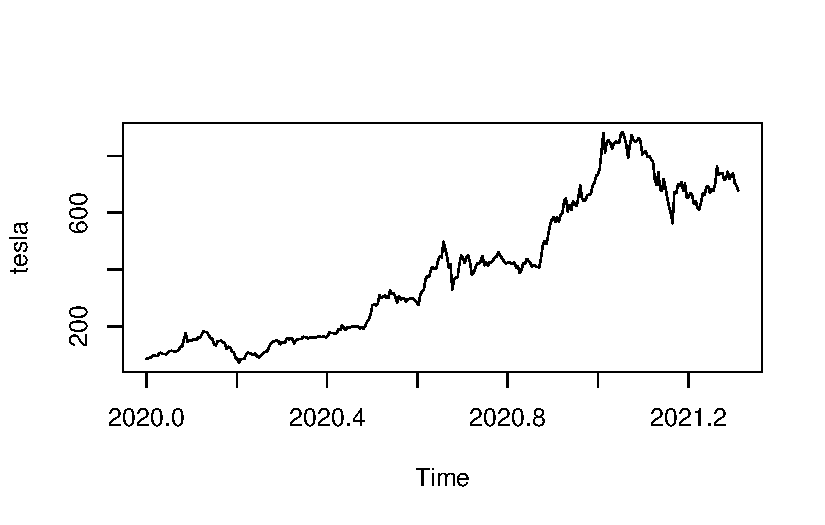
\includegraphics{series_files/figure-pdf/fig-charts-1.pdf}

}

\subcaption{\label{fig-charts-1}Precios de las acciones de Tesla}

\end{minipage}%
%
\begin{minipage}{0.33\linewidth}

\centering{

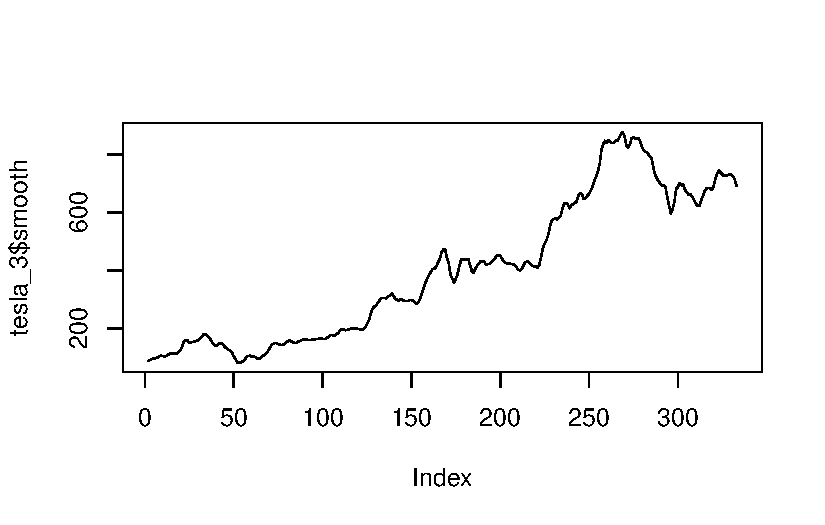
\includegraphics{series_files/figure-pdf/fig-charts-2.pdf}

}

\subcaption{\label{fig-charts-2}MA Smoother Tesla: Orden=3}

\end{minipage}%
%
\begin{minipage}{0.33\linewidth}

\centering{

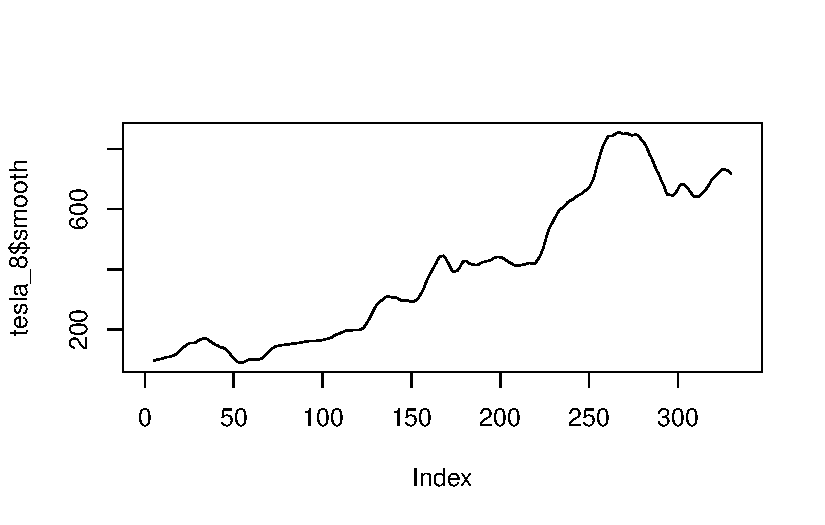
\includegraphics{series_files/figure-pdf/fig-charts-3.pdf}

}

\subcaption{\label{fig-charts-3}MA Smoother Tesla: Orden=8}

\end{minipage}%
\newline
\begin{minipage}{0.33\linewidth}

\centering{

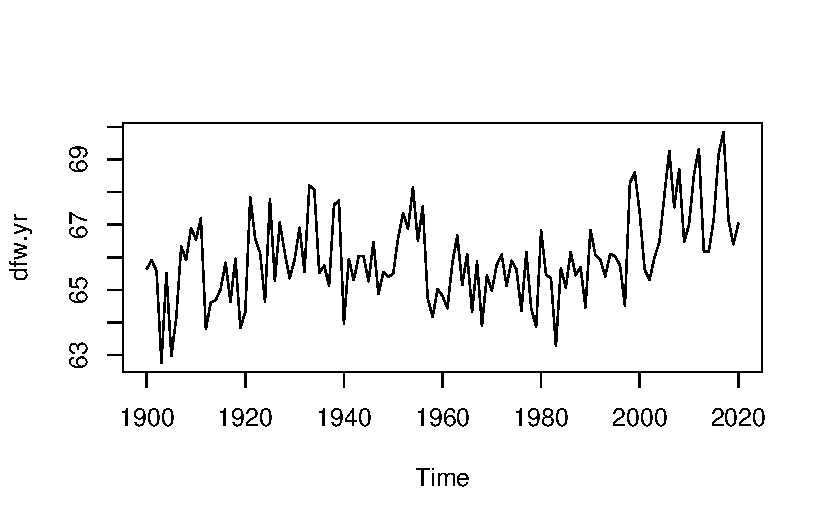
\includegraphics{series_files/figure-pdf/fig-charts-4.pdf}

}

\subcaption{\label{fig-charts-4}Temperatura anual DFW}

\end{minipage}%
%
\begin{minipage}{0.33\linewidth}

\centering{

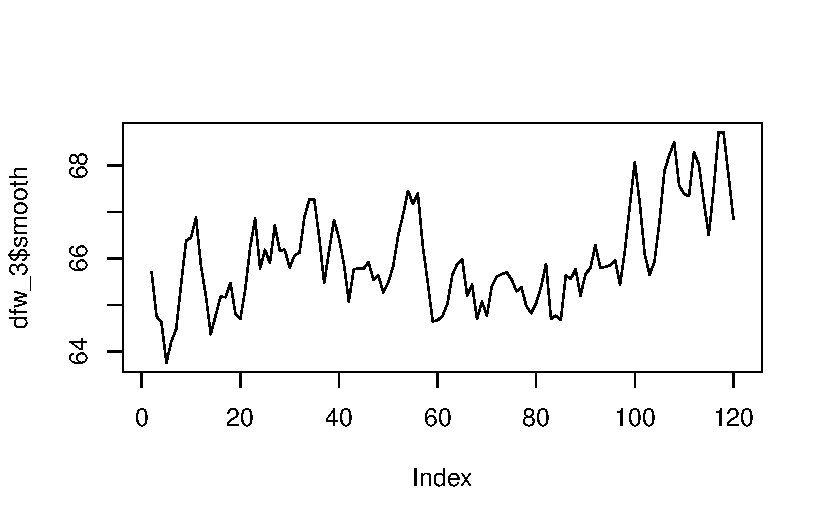
\includegraphics{series_files/figure-pdf/fig-charts-5.pdf}

}

\subcaption{\label{fig-charts-5}MA Smoother DFW: Orden=3}

\end{minipage}%
%
\begin{minipage}{0.33\linewidth}

\centering{

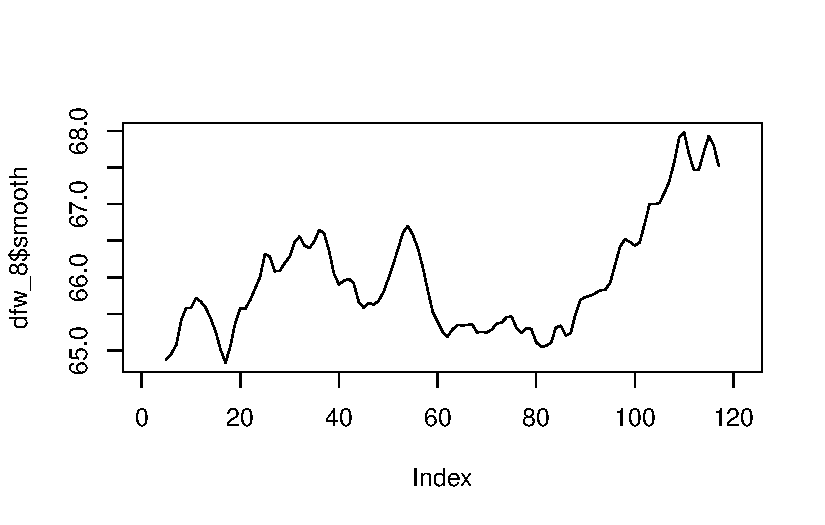
\includegraphics{series_files/figure-pdf/fig-charts-6.pdf}

}

\subcaption{\label{fig-charts-6}MA Smoother DFW: Orden=8}

\end{minipage}%

\caption{\label{fig-charts}Precios de las acciones de Tesla y datos de
temperatura anual de DFW antes y después de aplicar suavizadores de
promedio móvil de orden 3 y 8}

\end{figure}%

\end{tcolorbox}

\end{example}

\section{Análisis y técnicas de
descomposición.}\label{anuxe1lisis-y-tuxe9cnicas-de-descomposiciuxf3n.}

\subsection{Descomposición de datos
estacionales}\label{descomposiciuxf3n-de-datos-estacionales}

En el Ejemplo~\ref{exm-airpass} se aborda la naturaleza de los datos
estacionales, entendidos como una serie de datos cíclicos con periodos
consistentes y un patrón que guarda relación con el calendario. El
conjunto de datos de AirPassengers presentado en la
Figura~\ref{fig-airpass} se clasifica como un ejemplo paradigmático de
datos estacionales. Este conjunto de datos exhibe un comportamiento
estacional anual, además de una tendencia de crecimiento, que se
aproxima a ser lineal. Es convencional considerar que los datos
estacionales, denotados como \(x_{_t}\), comprenden:

\begin{enumerate}
\def\labelenumi{\alph{enumi}.}
\item
  Un componente estacional intrínseco anual, identificado como
  \(s_{_t}\),
\item
  Un componente de tendencia a largo plazo, referido como \(tr_{_t}\) y,
\item
  Un componente de variabilidad aleatoria, conocido como \(z_{_t}\).
\end{enumerate}

Se ha observado esta estructura en el conjuntos de datos ya mencionado.
Los expertos en análisis de series temporales se enfocan en dos
categorías de modelos estacionales:

\emph{Datos estacionales aditivos}

Los datos \(x_{_t}\), en el tiempo \(t\) pueden ser considerados como
una suma dada en la ecuación (\ref{eq-addseas})

\begin{equation}\phantomsection\label{eq-addseas}{
x_{_t}=s_{_t}+tr_{_t}+z_{_t}.
}\end{equation}

\emph{Datos estacionales multiplicativos}

Los datos, \(x_{_t}\), en el tiempo \(t\) pueden ser expresados como el
producto dado en la ecuación (\ref{eq-mulseas})

\begin{equation}\phantomsection\label{eq-mulseas}{
x_{_t}=s_{_t}\times tr_{_t}\times z_{_t}.
}\end{equation}

\begin{example}[]\protect\hypertarget{exm-air}{}\label{exm-air}

~

\begin{tcolorbox}[enhanced jigsaw, breakable, colbacktitle=quarto-callout-caution-color!10!white, rightrule=.15mm, toptitle=1mm, colback=white, left=2mm, colframe=quarto-callout-caution-color-frame, bottomtitle=1mm, opacitybacktitle=0.6, leftrule=.75mm, arc=.35mm, title={Datos de pasajeros aéreos}, coltitle=black, titlerule=0mm, opacityback=0, bottomrule=.15mm, toprule=.15mm]

Para ilustrar la diferencia entre los tipos de datos que se ajustan
mejor a un modelo aditivo y a uno multiplicativo, se utiliza el conjunto
de datos de AirPassengers. Como se ha señalado anteriormente, los datos
de AirPassengers, representados en la Figura~\ref{fig-air-1}, tienen un
componente estacional y de tendencia, pero también la variabilidad
dentro del año aumenta con el tiempo.

\begin{Shaded}
\begin{Highlighting}[]
\FunctionTok{library}\NormalTok{(tswge)}
\FunctionTok{data}\NormalTok{(AirPassengers)}
\NormalTok{logAirPassengers}\OtherTok{=}\FunctionTok{log}\NormalTok{(AirPassengers)}
\FunctionTok{plot}\NormalTok{(AirPassengers)}
\FunctionTok{plot}\NormalTok{(logAirPassengers)}
\end{Highlighting}
\end{Shaded}

\begin{figure}[H]

\begin{minipage}{0.50\linewidth}

\centering{

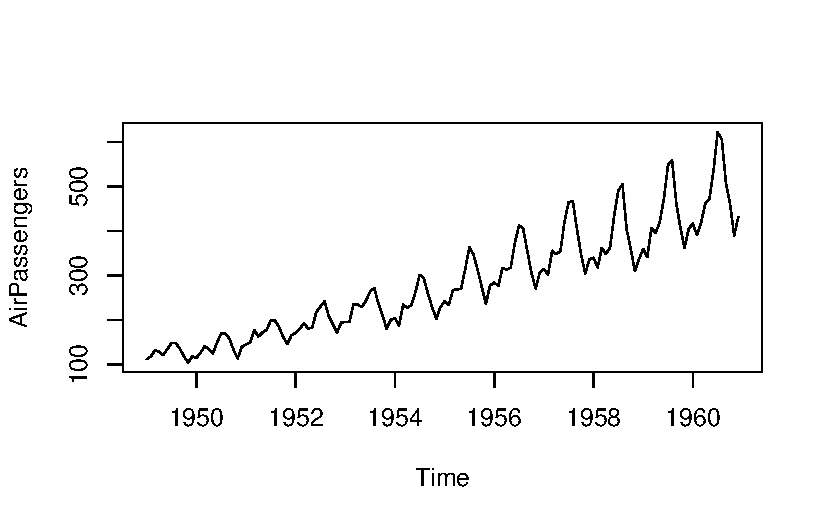
\includegraphics{series_files/figure-pdf/fig-air-1.pdf}

}

\subcaption{\label{fig-air-1}Datos de pasajeros aéreos: 1949-1960}

\end{minipage}%
%
\begin{minipage}{0.50\linewidth}

\centering{

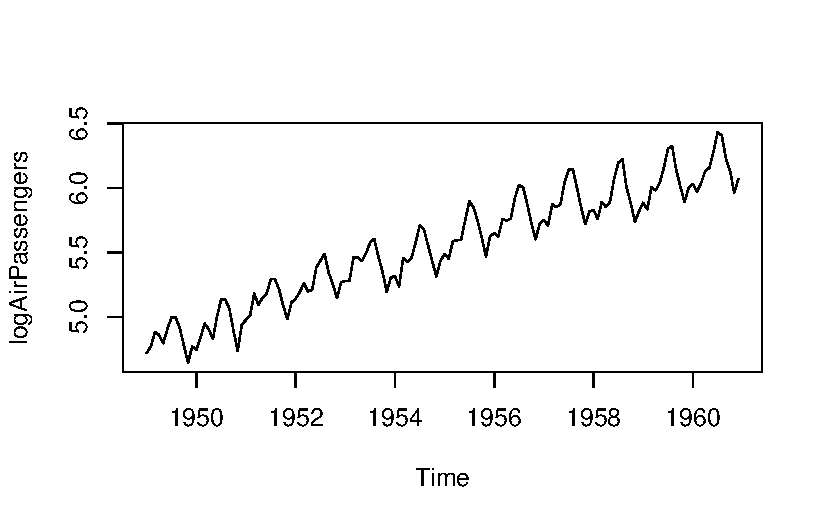
\includegraphics{series_files/figure-pdf/fig-air-2.pdf}

}

\subcaption{\label{fig-air-2}Datos de pasajeros aéreos en escala
logarítmica}

\end{minipage}%

\caption{\label{fig-air}Datos de pasajeros aereos y logaritmo de los
datos de pasajeros aereos}

\end{figure}%

Los conjuntos de datos con este tipo de comportamiento suelen modelarse
utilizando modelos multiplicativos. Para eliminar el aumento en la
variabilidad, los analistas suelen tomar el logaritmo de los datos y
utilizan los ``datos logarítmicos'' para el análisis.

Los datos logarítmicos de logAirPassengers en la Figura~\ref{fig-air-2}
no muestran un aumento en la variabilidad dentro del año y son un
ejemplo clásico de datos que se modelan utilizando el modelo aditivo en
la ecuación (\ref{eq-addseas}).

\end{tcolorbox}

\end{example}

Se comenzó discutiendo el modelo aditivo, considerado el más intuitivo
de los dos.

A continuación, se discutirán las diferencias en las estrategias de
modelado para estos dos conjuntos de datos.

Las descomposiciones aditivas y multiplicativas siguen pasos de
implementación similares:

\begin{enumerate}
\def\labelenumi{\arabic{enumi}.}
\tightlist
\item
  Estimar el componente de tendencia.
\item
  Eliminar el componente de tendencia, lo que resulta en un conjunto de
  datos compuesto principalmente por las fluctuaciones estacionales en
  los datos.
\item
  Calcular un componente estacional ``promedio'' dentro del año.
\item
  Encontrar el ruido restante.
\end{enumerate}

Se comenzará discutiendo el modelo aditivo, que es el más intuitivo de
los dos.

\subsubsection{Descomposición aditiva}\label{descomposiciuxf3n-aditiva}

Cuando se analizan datos utilizando el modelo aditivo en la ecuación
(\ref{eq-addseas}), se parte del supuesto de que los datos son la suma
de componentes estacionales, de tendencia y de ruido aleatorio. Se
discuten los pasos de análisis involucrados en la descomposición de los
datos logarítmicos de logAirPassengers. En la práctica, los componentes
en la ecuación (\ref{eq-addseas}) se estiman y un modelo estimado puede
describirse como

\begin{equation}\phantomsection\label{eq-addecompose}{
x_{_t}=\hat{s_{_t}}+\hat{tr_{_t}}+\hat{z_{_t}}.
}\end{equation}

\begin{example}[]\protect\hypertarget{exm-logair}{}\label{exm-logair}

~

\begin{tcolorbox}[enhanced jigsaw, breakable, colbacktitle=quarto-callout-caution-color!10!white, rightrule=.15mm, toptitle=1mm, colback=white, left=2mm, colframe=quarto-callout-caution-color-frame, bottomtitle=1mm, opacitybacktitle=0.6, leftrule=.75mm, arc=.35mm, title={Descomposición aditiva de LogAirPassengers}, coltitle=black, titlerule=0mm, opacityback=0, bottomrule=.15mm, toprule=.15mm]

La descomposición de los datos logAirPassengers se logra mediante los
siguientes pasos.

\begin{enumerate}
\def\labelenumi{\alph{enumi}.}
\item
  \textbf{\emph{Estimar el Componente de Tendencia}}: La
  Figura~\ref{fig-sm12} es una representación gráfica del conjunto de
  datos logAirPassengers superpuesto con el resultado de aplicar un
  suavizador de media móvil centrada de orden 12 a los datos.

\begin{Shaded}
\begin{Highlighting}[]
\FunctionTok{library}\NormalTok{(tswge)}
\FunctionTok{data}\NormalTok{(AirPassengers)}
\NormalTok{logAirPassengers}\OtherTok{=}\FunctionTok{log}\NormalTok{(AirPassengers)}
\NormalTok{logair}\FloatTok{.12}\OtherTok{=}\FunctionTok{ma.smooth.wge}\NormalTok{(logAirPassengers,}\AttributeTok{order=}\DecValTok{12}\NormalTok{)}
\NormalTok{logair}\FloatTok{.12}\SpecialCharTok{$}\NormalTok{smooth}
\end{Highlighting}
\end{Shaded}

\begin{verbatim}
  [1]       NA       NA       NA       NA       NA       NA 4.837280 4.841114
  [9] 4.846596 4.851238 4.854488 4.859954 4.869840 4.881389 4.893411 4.904293
 [17] 4.912752 4.923701 4.940483 4.957406 4.974380 4.991942 5.013095 5.033804
 [25] 5.047776 5.060902 5.073812 5.088378 5.106906 5.124312 5.138282 5.152751
 [33] 5.163718 5.171454 5.178401 5.189431 5.203909 5.218093 5.231553 5.243722
 [41] 5.257413 5.270736 5.282916 5.292150 5.304079 5.323338 5.343560 5.357427
 [49] 5.367695 5.378309 5.388417 5.397805 5.403849 5.407220 5.410364 5.410294
 [57] 5.408381 5.406761 5.406218 5.410571 5.419628 5.428330 5.435128 5.442237
 [65] 5.450659 5.461103 5.473655 5.489713 5.503974 5.516367 5.529403 5.542725
 [73] 5.557864 5.572693 5.587498 5.602730 5.616658 5.631189 5.645937 5.659812
 [81] 5.674172 5.687636 5.700766 5.714738 5.727153 5.738856 5.750676 5.760658
 [89] 5.770846 5.780430 5.788745 5.796524 5.804821 5.814072 5.823075 5.832692
 [97] 5.842665 5.853541 5.864863 5.875490 5.885654 5.894475 5.901555 5.907026
[105] 5.910012 5.910708 5.911637 5.913829 5.917360 5.922887 5.926146 5.927563
[113] 5.929657 5.930458 5.932964 5.938377 5.946188 5.956352 5.967813 5.977291
[121] 5.985269 5.994078 6.003991 6.014899 6.026589 6.040709 6.054492 6.066195
[129] 6.073088 6.080733 6.091930 6.102013 6.112511 6.121153 6.128381 6.137437
[137] 6.145733 6.151526       NA       NA       NA       NA       NA       NA
\end{verbatim}

\begin{Shaded}
\begin{Highlighting}[]
\NormalTok{logair.sm12}\OtherTok{=}\FunctionTok{ts}\NormalTok{(logair}\FloatTok{.12}\SpecialCharTok{$}\NormalTok{smooth,}\AttributeTok{start=}\FunctionTok{c}\NormalTok{(}\DecValTok{1949}\NormalTok{,}\DecValTok{1}\NormalTok{),}\AttributeTok{frequency=}\DecValTok{12}\NormalTok{)}
\end{Highlighting}
\end{Shaded}

  \begin{figure}[H]

  \centering{

  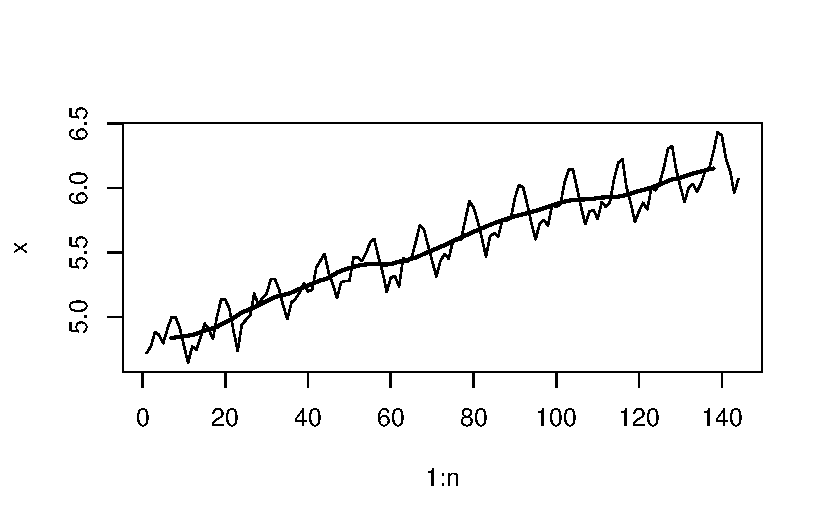
\includegraphics{series_files/figure-pdf/fig-sm12-1.pdf}

  }

  \caption{\label{fig-sm12}LogAirPassengers con un suavizador de
  promedio móvil centrado de orden 12.}

  \end{figure}%

  En relación con el modelo estimado en la ecuación
  (\ref{eq-addecompose}), \(\hat{tr_{_t}} =\) \textbf{logair.sm12}
  representa la curva casi lineal en la Figura~\ref{fig-sm12}.
\item
  \textbf{\emph{Eliminar el Componente de Tendencia de los Datos:}} El
  paso subsiguiente implica la sustracción del componente de tendencia
  estimado de los datos (logAirPassengers).

\begin{Shaded}
\begin{Highlighting}[]
\NormalTok{seas.logair}\OtherTok{=}\NormalTok{logAirPassengers}\SpecialCharTok{{-}}\NormalTok{logair.sm12}
\FunctionTok{round}\NormalTok{(seas.logair,}\DecValTok{4}\NormalTok{) }
\end{Highlighting}
\end{Shaded}

\begin{verbatim}
         Jan     Feb     Mar     Apr     May     Jun     Jul     Aug     Sep
1949      NA      NA      NA      NA      NA      NA  0.1599  0.1561  0.0661
1950 -0.1249 -0.0451  0.0553  0.0010 -0.0844  0.0802  0.1953  0.1784  0.0882
1951 -0.0710 -0.0503  0.1080  0.0054  0.0406  0.0575  0.1550  0.1406  0.0512
1952 -0.0622 -0.0251  0.0311 -0.0452 -0.0479  0.1138  0.1552  0.1968  0.0383
1953 -0.0896 -0.1002  0.0754  0.0618  0.0299  0.0858  0.1656  0.1955  0.0597
1954 -0.1015 -0.1919  0.0245 -0.0173  0.0047  0.1148  0.2368  0.1905  0.0529
1955 -0.0689 -0.1217 -0.0002 -0.0080 -0.0182  0.1214  0.2512  0.1895  0.0688
1956 -0.0782 -0.1148  0.0082 -0.0145 -0.0088  0.1438  0.2347  0.2074  0.0673
1957 -0.0901 -0.1464  0.0101 -0.0233 -0.0135  0.1505  0.2405  0.2393  0.0914
1958 -0.0884 -0.1608 -0.0345 -0.0754 -0.0353  0.1449  0.2635  0.2862  0.0552
1959 -0.0992 -0.1593  0.0024 -0.0335  0.0137  0.1163  0.2518  0.2600  0.0646
1960 -0.0794 -0.1524 -0.0905 -0.0040  0.0112  0.1307      NA      NA      NA
         Oct     Nov     Dec
1949 -0.0721 -0.2101 -0.0893
1950 -0.1016 -0.2769 -0.0922
1951 -0.0839 -0.1948 -0.0774
1952 -0.0711 -0.1961 -0.0896
1953 -0.0549 -0.2133 -0.1073
1954 -0.0826 -0.2162 -0.1090
1955 -0.0745 -0.2327 -0.0871
1956 -0.0905 -0.2210 -0.1091
1957 -0.0614 -0.1913 -0.0967
1958 -0.0730 -0.2312 -0.1572
1959 -0.0719 -0.2003 -0.0981
1960      NA      NA      NA
\end{verbatim}
\end{enumerate}

\begin{figure}[H]

\begin{minipage}{0.50\linewidth}

\centering{

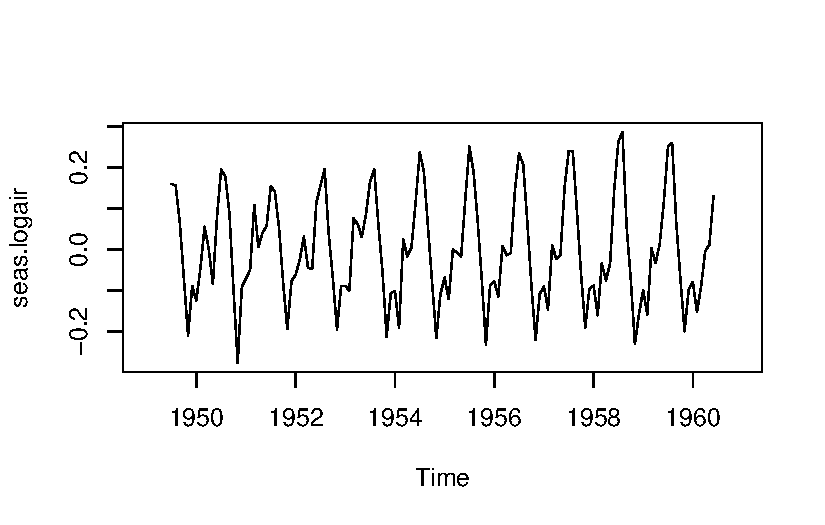
\includegraphics{series_files/figure-pdf/fig-seasair-1.pdf}

}

\subcaption{\label{fig-seasair-1}LogAirPassengers sin tendencia}

\end{minipage}%
%
\begin{minipage}{0.50\linewidth}

\centering{

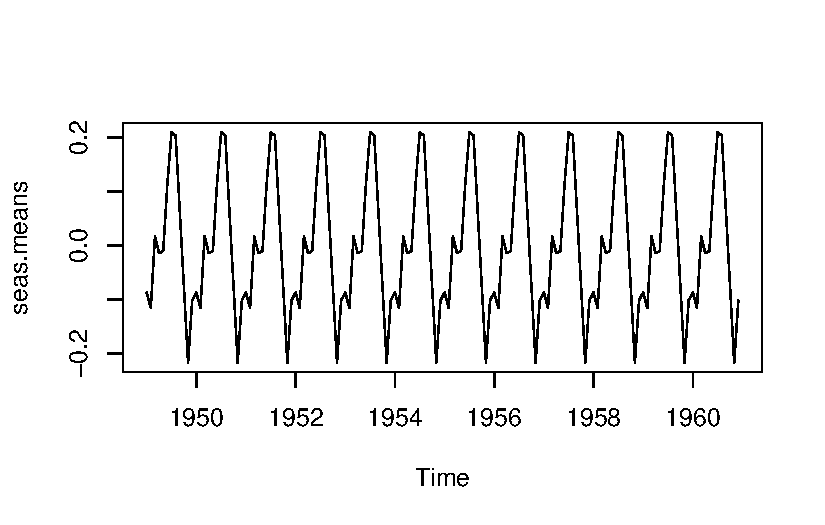
\includegraphics{series_files/figure-pdf/fig-seasair-2.pdf}

}

\subcaption{\label{fig-seasair-2}Componente estacional estimado}

\end{minipage}%

\caption{\label{fig-seasair}Datos de LogAirPassengers sin el componente
de tendencia y componente estacional estimado.}

\end{figure}%

Se aprecia con mayor claridad el comportamiento estacional año tras año
en la Figura~\ref{fig-seasair-1} sin la ``interferencia'' de la
tendencia. Específicamente, se observa un patrón similar en cada año
(mayor cantidad de viajes en verano, disminución en noviembre, aún bajos
pero con una ligera alza en diciembre, continuamente bajos en enero y
febrero, alza en marzo, y así sucesivamente). No obstante, se presentan
variaciones de un año a otro: los viajes aéreos en noviembre fueron
notablemente bajos en 1950 y luego inusualmente altos en julio y agosto
de 1958.

\begin{enumerate}
\def\labelenumi{\alph{enumi}.}
\setcounter{enumi}{2}
\item
  \textbf{\emph{Calcular un ``Promedio'' del Componente Estacional
  Dentro del Año:}} Es importante notar que, el componente estacional en
  el modelo (ecuación (\ref{eq-addseas})), es un patrón general que se
  mantiene igual de un año a otro. Es
  decir,\(\{s_{_t}, t=1,\ldots,12\} = \{s_{_{t+12}},t=1,\ldots,12\} =\{s_{_{t+2(12)}}, t=1,\ldots,12\}=\cdots.\)
  El componente de ruido, \(z_{_t}\), ajusta las variaciones de un año a
  otro del patrón estacional general. El patrón estacional,
  \(s_{_t}, t=1,\ldots,12\), se estima calculando el promedio a lo largo
  de los años y, el componente estacional estimado, \(\hat{s}_{_t}\) (el
  cual es el mismo para cada año), se muestra en la
  Figura~\ref{fig-seasair-2}.

\begin{Shaded}
\begin{Highlighting}[]
\NormalTok{seas.logair.numeric}\OtherTok{=}\FunctionTok{as.numeric}\NormalTok{(seas.logair)}
\NormalTok{seas.logair.matrix}\OtherTok{=}\FunctionTok{matrix}\NormalTok{(seas.logair.numeric,}\AttributeTok{ncol=}\DecValTok{12}\NormalTok{)}
\NormalTok{seas.logair.matrix.t}\OtherTok{=}\FunctionTok{t}\NormalTok{(seas.logair.matrix)}
\NormalTok{months}\OtherTok{=}\FunctionTok{colMeans}\NormalTok{(seas.logair.matrix.t, }\AttributeTok{na.rm=}\ConstantTok{TRUE}\NormalTok{)}
\FunctionTok{round}\NormalTok{(months,}\DecValTok{4}\NormalTok{)}
\end{Highlighting}
\end{Shaded}

\begin{verbatim}
 [1] -0.0867 -0.1153  0.0172 -0.0139 -0.0098  0.1145  0.2100  0.2036  0.0640
[10] -0.0761 -0.2167 -0.1012
\end{verbatim}

\begin{Shaded}
\begin{Highlighting}[]
\NormalTok{seas.means}\OtherTok{=}\FunctionTok{rep}\NormalTok{(months,}\DecValTok{12}\NormalTok{)}
\NormalTok{seas.means}\OtherTok{=}\FunctionTok{ts}\NormalTok{(seas.means,}\AttributeTok{start=}\FunctionTok{c}\NormalTok{(}\DecValTok{1949}\NormalTok{,}\DecValTok{1}\NormalTok{),}\AttributeTok{frequency=}\DecValTok{12}\NormalTok{)}
\end{Highlighting}
\end{Shaded}
\item
  \textbf{\emph{Encontrar el componente de ruido restante:}} El ruido
  estimado en la ecuación (\ref{eq-addecompose}), \(\hat{z_{_t}}\), es
  calculado de la siguiente manera

\begin{Shaded}
\begin{Highlighting}[]
\NormalTok{logair.noise }\OtherTok{=}\NormalTok{ logAirPassengers }\SpecialCharTok{{-}}\NormalTok{ logair.sm12 }\SpecialCharTok{{-}}\NormalTok{ seas.means}
\FunctionTok{plot}\NormalTok{(}\FunctionTok{decompose}\NormalTok{(logAirPassengers))}
\end{Highlighting}
\end{Shaded}

  \begin{figure}[H]

  \centering{

  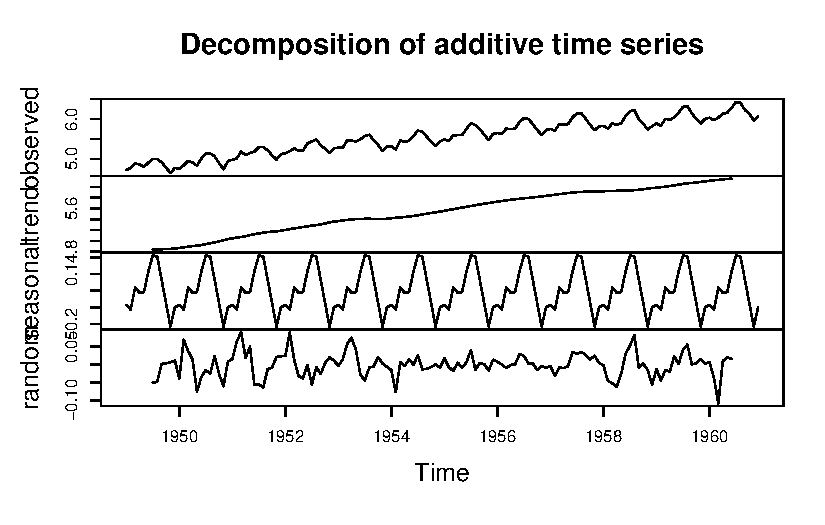
\includegraphics{series_files/figure-pdf/fig-descadd-1.pdf}

  }

  \caption{\label{fig-descadd}Descomposición aditiva de
  LogAirPassengers.}

  \end{figure}%
\end{enumerate}

La Figura~\ref{fig-descadd} muestra un gráfico de los datos de
LogAirPassengers junto con las partes del procedimiento de
descomposición.

\end{tcolorbox}

\end{example}

\subsubsection{Descomposición
multiplicativa}\label{descomposiciuxf3n-multiplicativa}

Se llevará a cabo en el Ejemplo~\ref{exm-mulair} una descomposición
multiplicativa de los datos de AirPassengers. Se destaca que esta serie
temporal exhibe un patrón estacional y una variabilidad intra-anual
crecientes con el tiempo. A pesar de la posibilidad de modelar estos
datos mediante el uso del logaritmo seguido de un modelo aditivo, en
esta sección se opta por un enfoque multiplicativo para analizar los
datos originales de AirPassengers. Al emplear la descomposición
multiplicativa en el análisis de datos, se hace la suposición de que la
serie temporal es el resultado de componentes estacionales, de tendencia
y de ruido. El modelo estimado se expresa como;

\begin{equation}\phantomsection\label{eq-muldecom}{
x_{_t}=\hat{s_{_t}}\times \hat{tr_{_t}}\times \hat{z_{_t}}.
}\end{equation}

\begin{example}[]\protect\hypertarget{exm-mulair}{}\label{exm-mulair}

~

\begin{tcolorbox}[enhanced jigsaw, breakable, colbacktitle=quarto-callout-caution-color!10!white, rightrule=.15mm, toptitle=1mm, colback=white, left=2mm, colframe=quarto-callout-caution-color-frame, bottomtitle=1mm, opacitybacktitle=0.6, leftrule=.75mm, arc=.35mm, title={Descomposición multiplicativa de AirPassengers}, coltitle=black, titlerule=0mm, opacityback=0, bottomrule=.15mm, toprule=.15mm]

\begin{enumerate}
\def\labelenumi{\alph{enumi}.}
\item
  \textbf{\emph{Estimar el Componente de Tendencia}}: Al igual que con
  el modelo aditivo, el primer paso consiste en utilizar un suavizador
  de media móvil centrada, nuevamente en este caso de orden 12.
  Anteriormente se calculó y representó gráficamente el suavizador de
  media móvil en la Figura~\ref{fig-smap}.

\begin{Shaded}
\begin{Highlighting}[]
\FunctionTok{library}\NormalTok{(tswge)}
\FunctionTok{data}\NormalTok{(AirPassengers)}
\NormalTok{AirPass.sm12}\OtherTok{=}\FunctionTok{ma.smooth.wge}\NormalTok{(AirPassengers,}\AttributeTok{order=}\DecValTok{12}\NormalTok{)}
\NormalTok{AirPass.sm12}\OtherTok{=}\FunctionTok{ts}\NormalTok{(AirPass.sm12}\SpecialCharTok{$}\NormalTok{smooth,}\AttributeTok{start=}\FunctionTok{c}\NormalTok{(}\DecValTok{1949}\NormalTok{,}\DecValTok{1}\NormalTok{),}\AttributeTok{frequency=}\DecValTok{12}\NormalTok{)}
\end{Highlighting}
\end{Shaded}

  \begin{figure}[H]

  \centering{

  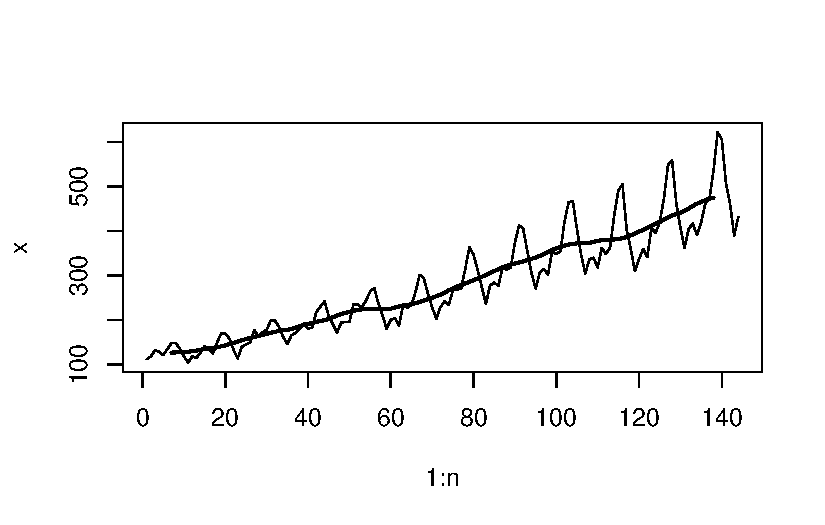
\includegraphics{series_files/figure-pdf/fig-smap-1.pdf}

  }

  \caption{\label{fig-smap}Datos de pasajeros aéreos con suavizado de
  orden 12.}

  \end{figure}%

  Es importante recordar que, en relación con el modelo estimado en la
  ecuación (\ref{eq-muldecom}), \(\hat{tr_{_t}} =\)
  \textbf{AirPass.sm12}. Esta curva casi lineal se muestra como parte de
  la descomposición completa en la Figura~\ref{fig-descmul}.
\item
  \textbf{\emph{Eliminar el Componente de Tendencia de los Datos:}} El
  siguiente paso consiste en eliminar el componente de tendencia
  estimado del conjunto de datos de AirPassengers. Esto se puede lograr
  mediante la división (en lugar de la resta).

\begin{Shaded}
\begin{Highlighting}[]
\NormalTok{seas.AirPass}\OtherTok{=}\NormalTok{AirPassengers}\SpecialCharTok{/}\NormalTok{AirPass.sm12}
\end{Highlighting}
\end{Shaded}

  La conducta estacional de un año a otro resulta mucho más clara en la
  Figura~\ref{fig-seasmul-1} después de eliminar la ``interferencia'' de
  la tendencia y el aumento de la variabilidad dentro del año. También
  se observa que la variabilidad dentro del año no está aumentando tanto
  como en la Figura~\ref{fig-airpass}. El incremento en la variabilidad
  en el modelo final (ecuación (\ref{eq-muldecom})) se debe a la
  tendencia creciente que se multiplica por los datos estacionales en la
  Figura~\ref{fig-seasmul-1}. Los patrones estacionales en la
  Figura~\ref{fig-seasmul-1} son similares a los de los datos aditivos
  mostrados en la Figura~\ref{fig-seasair-1}.
\end{enumerate}

\begin{figure}[H]

\begin{minipage}{0.50\linewidth}

\centering{

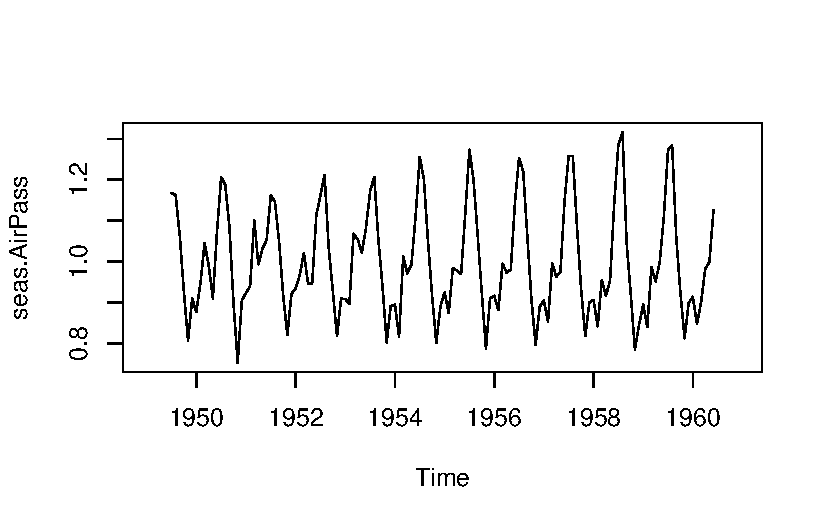
\includegraphics{series_files/figure-pdf/fig-seasmul-1.pdf}

}

\subcaption{\label{fig-seasmul-1}AirPassengers Datos/tendencia}

\end{minipage}%
%
\begin{minipage}{0.50\linewidth}

\centering{

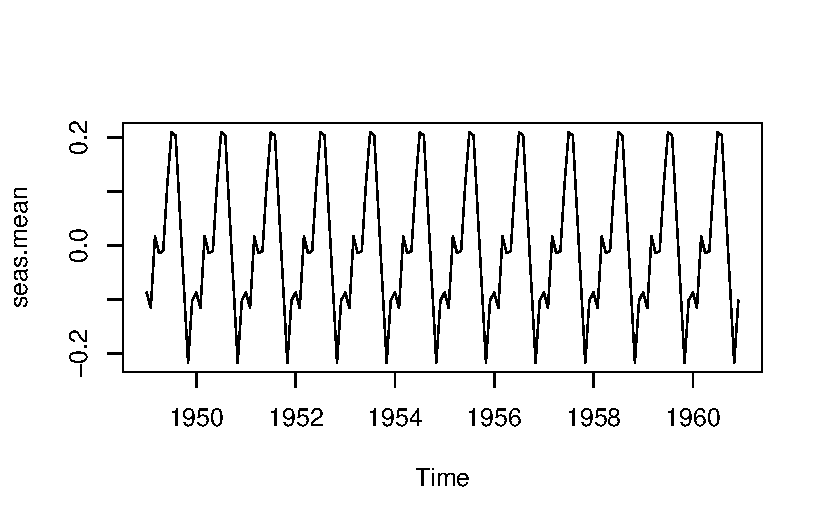
\includegraphics{series_files/figure-pdf/fig-seasmul-2.pdf}

}

\subcaption{\label{fig-seasmul-2}Componente estacional estimado}

\end{minipage}%

\caption{\label{fig-seasmul}Datos de AirPassengers sin el componente de
tendencia y componente estacional estimado.}

\end{figure}%

\begin{enumerate}
\def\labelenumi{\alph{enumi}.}
\setcounter{enumi}{2}
\item
  \textbf{\emph{Calcular un ``Promedio'' del Componente Estacional
  Dentro del Año:}} Al igual que en el modelo aditivo, en el modelo
  \ref{eq-mulseas}, el componente estacional es un patrón general que se
  supone igual de un año a otro, y el componente de ruido, \(z_{_t}\),
  se ajusta a las variaciones de un año a otro con respecto al patrón
  estacional general. El componente estacional estimado,
  \(\hat{s_{_t}}\) (que es idéntico para cada año), se representa en la
  Figura~\ref{fig-seasmul-2}. Se observa la similitud entre la
  Figura~\ref{fig-seasmul-2} y la Figura~\ref{fig-seasair-2}, que fue el
  componente estacional para la descomposición aditiva de los datos
  logAirPassengers.

\begin{Shaded}
\begin{Highlighting}[]
\NormalTok{seas.AirPass.numeric}\OtherTok{=}\FunctionTok{as.numeric}\NormalTok{(seas.AirPass) }
\NormalTok{seas.AirPass.matrix}\OtherTok{=}\FunctionTok{matrix}\NormalTok{(seas.AirPass.numeric,}\AttributeTok{ncol=}\DecValTok{12}\NormalTok{) }
\NormalTok{seas.AirPass.matrix.t}\OtherTok{=}\FunctionTok{t}\NormalTok{(seas.AirPass.matrix) }
\NormalTok{months}\OtherTok{=}\FunctionTok{colMeans}\NormalTok{(seas.AirPass.matrix.t,}\AttributeTok{na.rm=}\ConstantTok{TRUE}\NormalTok{) }
\NormalTok{seas.means}\OtherTok{=}\FunctionTok{rep}\NormalTok{(months,}\DecValTok{12}\NormalTok{) }
\NormalTok{seas.means}\OtherTok{=}\FunctionTok{ts}\NormalTok{(seas.means,}\AttributeTok{start=}\FunctionTok{c}\NormalTok{(}\DecValTok{1949}\NormalTok{,}\DecValTok{1}\NormalTok{),}\AttributeTok{frequency=}\DecValTok{12}\NormalTok{)}
\end{Highlighting}
\end{Shaded}
\item
  \textbf{\emph{Encontrar el componente de ruido restante:}} El ruido
  estimado en la ecuación (\ref{eq-muldecom}), \(\hat{z_{_t}}\), es
  calculado de la siguiente manera

\begin{Shaded}
\begin{Highlighting}[]
\NormalTok{Air.Pass.noise }\OtherTok{=}\NormalTok{ AirPassengers }\SpecialCharTok{/}\NormalTok{ (AirPass.sm12 }\SpecialCharTok{*}\NormalTok{ seas.mean)}
\FunctionTok{plot}\NormalTok{(}\FunctionTok{decompose}\NormalTok{(AirPassengers))}
\end{Highlighting}
\end{Shaded}

  \begin{figure}[H]

  \centering{

  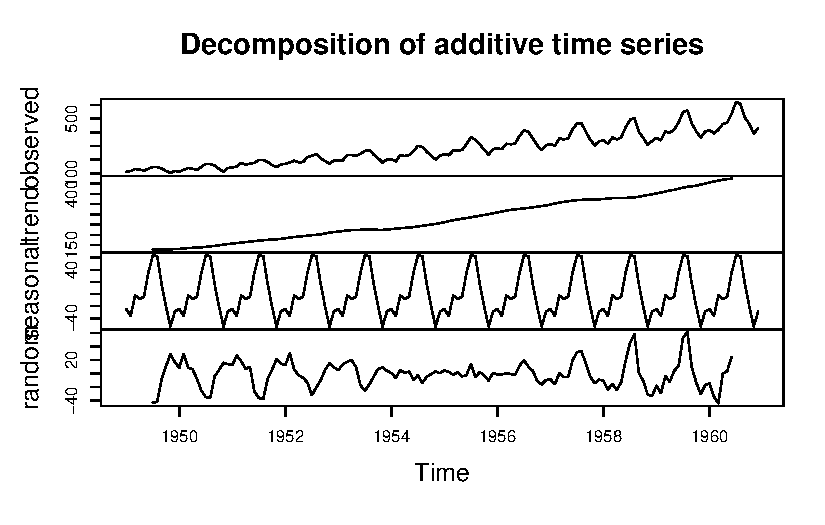
\includegraphics{series_files/figure-pdf/fig-descmul-1.pdf}

  }

  \caption{\label{fig-descmul}Descomposición multiplicativa de
  AirPassengers.}

  \end{figure}%
\end{enumerate}

La Figura~\ref{fig-descmul} muestra un gráfico de los datos de
AirPassengers junto con las partes del procedimiento de descomposición.

\end{tcolorbox}

\end{example}

\subsection{Ajuste estacional}\label{ajuste-estacional}

\subsubsection{Ajuste estacional
aditivo}\label{ajuste-estacional-aditivo}

Los ajustes estacionales están relacionados con las descomposiciones
discutidas previamente. Si una descomposición aditiva es apropiada,
entonces se utiliza un ajuste estacional aditivo. Un emparejamiento
similar se aplica en el caso multiplicativo. El método de ajuste
estacional aditivo más directo, consiste en obtener los datos ajustados
estacionalmente, \(\hat{sa_{_t}}\), utilizando la fórmula

\begin{equation}\phantomsection\label{eq-AEadd}{
\hat{sa_{_t}}=x_{_t}-\hat{s_{_t}},
}\end{equation}

que resta el componente estacional (mostrado en la
Figura~\ref{fig-seasair-2}) de los datos.

\subsubsection{Ajuste estacional
multiplicativo}\label{ajuste-estacional-multiplicativo}

Dado que la descomposición multiplicativa fue apropiada para los datos
de pasajeros aéreos, se empleará un ajuste estacional multiplicativo
para este conjunto de datos. Similar al método utilizado para el ajuste
estacional aditivo, los datos ajustados estacionalmente utilizan la
fórmula

\begin{equation}\phantomsection\label{eq-AEMul}{
\hat{sa_{_t}}=x_{_t}/\hat{s_{_t}},
}\end{equation}

para dividir los datos por el componente estacional (mostrado en la
Figura~\ref{fig-seasmul-2}).

\begin{example}[]\protect\hypertarget{exm-aeair}{}\label{exm-aeair}

~

\begin{tcolorbox}[enhanced jigsaw, breakable, colbacktitle=quarto-callout-caution-color!10!white, rightrule=.15mm, toptitle=1mm, colback=white, left=2mm, colframe=quarto-callout-caution-color-frame, bottomtitle=1mm, opacitybacktitle=0.6, leftrule=.75mm, arc=.35mm, title={AirPassengers}, coltitle=black, titlerule=0mm, opacityback=0, bottomrule=.15mm, toprule=.15mm]

La Figura~\ref{fig-AEmul-1} muestra los datos de Pasajeros Aéreos
superpuestos con la estimación de tendencia obtenida utilizando un
suavizador de media móvil centrada de orden 12. La
Figura~\ref{fig-AEmul-2} es una representación gráfica de los datos
ajustados estacionalmente calculados utilizando la ecuación
(\ref{eq-AEMul}). Es decir, es una representación de
\textbf{AirPassengers.adj}. Una vez más, los datos ajustados
estacionalmente son similares a la tendencia estimada pero con más
detalle respecto a los cambios mensuales.

El análisis de la Figura~\ref{fig-AEmul-3} muestra que, el ajuste
estacional utilizando \textbf{seas,} es más suave y se ve menos afectado
por el aumento de la variabilidad dentro del año en años posteriores. En
general, los resultados son similares a los vistos en la
Figura~\ref{fig-AEmul-2} con los efectos estacionales eliminados.

\begin{Shaded}
\begin{Highlighting}[]
\NormalTok{AirPassengers.adj }\OtherTok{=}\NormalTok{ AirPassengers}\SpecialCharTok{/}\NormalTok{seas.means}
\FunctionTok{library}\NormalTok{(seasonal) }
\FunctionTok{library}\NormalTok{(tswge)}
\FunctionTok{data}\NormalTok{(AirPassengers)}
\NormalTok{AirPass.sm12}\OtherTok{=}\FunctionTok{ma.smooth.wge}\NormalTok{(AirPassengers,}\AttributeTok{order=}\DecValTok{12}\NormalTok{)}
\NormalTok{AirPass.sm12}\OtherTok{=}\FunctionTok{ts}\NormalTok{(AirPass.sm12}\SpecialCharTok{$}\NormalTok{smooth,}\AttributeTok{start=}\FunctionTok{c}\NormalTok{(}\DecValTok{1949}\NormalTok{,}\DecValTok{1}\NormalTok{),}\AttributeTok{frequency=}\DecValTok{12}\NormalTok{)}
\NormalTok{census}\OtherTok{=}\FunctionTok{seas}\NormalTok{(AirPassengers)}
\FunctionTok{plot}\NormalTok{(AirPassengers.adj)}
\FunctionTok{plot}\NormalTok{(census}\SpecialCharTok{$}\NormalTok{data[,}\DecValTok{3}\NormalTok{])}
\end{Highlighting}
\end{Shaded}

\begin{figure}[H]

\begin{minipage}{0.33\linewidth}

\centering{

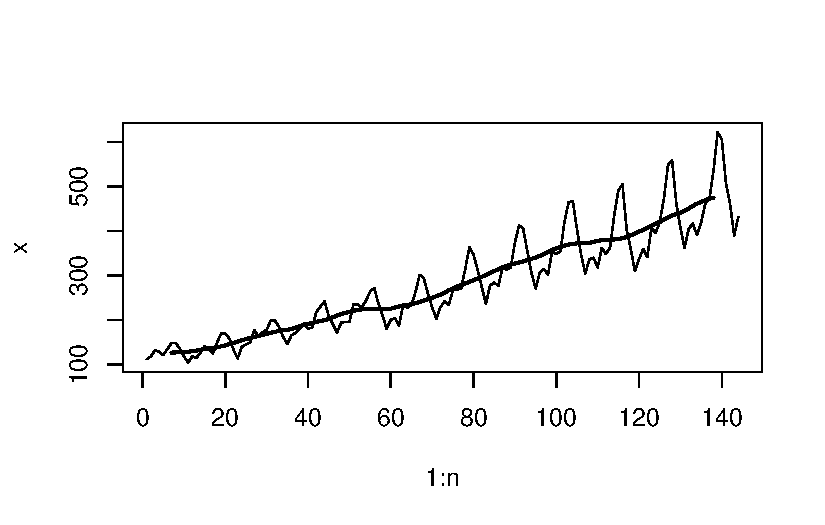
\includegraphics{series_files/figure-pdf/fig-AEmul-1.pdf}

}

\subcaption{\label{fig-AEmul-1}AirPassengers con suavizamiento}

\end{minipage}%
%
\begin{minipage}{0.33\linewidth}

\centering{

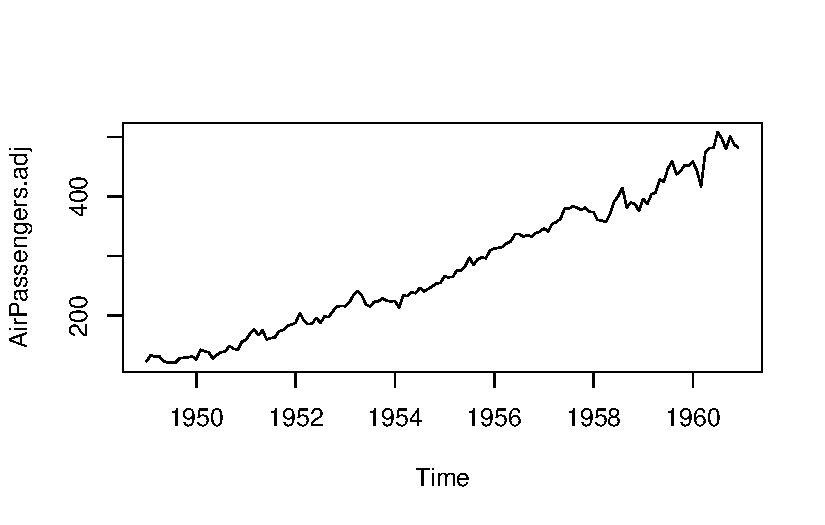
\includegraphics{series_files/figure-pdf/fig-AEmul-2.pdf}

}

\subcaption{\label{fig-AEmul-2}Ajuste estacional usando la fórmula}

\end{minipage}%
%
\begin{minipage}{0.33\linewidth}

\centering{

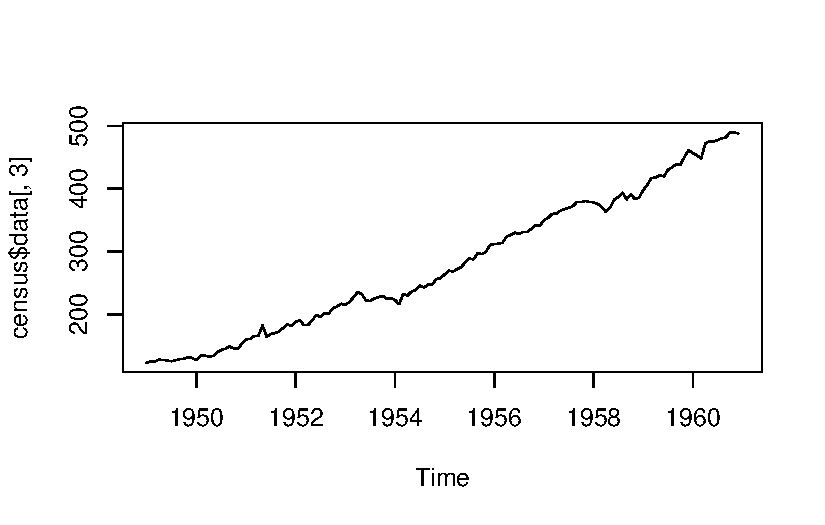
\includegraphics{series_files/figure-pdf/fig-AEmul-3.pdf}

}

\subcaption{\label{fig-AEmul-3}Ajuste estacional: Census}

\end{minipage}%

\caption{\label{fig-AEmul}Datos de AirPassengers y ajuste estacional
multiplicativo.}

\end{figure}%

\end{tcolorbox}

\end{example}

\section{Pronóstico y métodos
predictivos.}\label{pronuxf3stico-y-muxe9todos-predictivos.}

Una aplicación principal del análisis de series temporales es la de
realizar pronósticos. Anteriormente se mencionó que uno de los
propósitos del suavizado es prever valores futuros. De hecho, si existe
evidencia de que los patrones previos en un conjunto de datos
continuarán en el futuro, se pueden utilizar diversas técnicas para
realizar pronósticos.

Por ejemplo, un propietario de negocio puede desear prever la demanda
futura de cierto producto para asegurarse de tener la cantidad apropiada
de inventario en stock. Una ciudad que toma decisiones sobre
infraestructura podría necesitar prever su población en diez años. Un
problema difícil pero de interés para muchos en el sector financiero (y
para la mayoría de las personas, en realidad) es predecir las
fluctuaciones del mercado de valores y de las acciones individuales para
que se puedan tomar decisiones de inversión sólidas. Cada uno de estos
ejemplos ilustra la aplicabilidad y necesidad de técnicas de pronóstico.
Sin una opción mejor, dichos pronósticos a menudo se hacen de manera
algo subjetiva, basados en la memoria pasada de eventos similares,
rumores o tal vez mediante cálculos intuitivos pero presumidos que
proporcionan conjeturas educadas y estimaciones.

Afortunadamente, las técnicas de análisis de series temporales
proporcionan una alternativa matemática basada en si las suposiciones
matemáticas subyacentes son apropiadas. Esto resulta en algoritmos que
calculan pronósticos junto con límites de predicción correspondientes a
un determinado nivel de confianza, análogos al cálculo de la media
muestral más o menos un margen de error en el entorno de muestra
aleatoria no temporal. El escenario típico es que se desarrolle un
algoritmo de pronóstico que luego se utilice para predecir un resultado
de interés. El pronóstico comprende estimaciones de parámetros que
pueden encontrarse utilizando software en un esfuerzo por lograr una
capacidad predictiva óptima.

\begin{remark}
Se utilizarán los términos predicción y pronóstico de manera sinónima.
\end{remark}

\subsection{Suavizador de media móvil
predictivo}\label{suavizador-de-media-muxf3vil-predictivo}

En la Sección~\ref{sec-mas} se explicó cómo se utiliza el suavizador de
media móvil centrada para visualizar una versión suavizada de los datos
con el propósito de recuperar señales subyacentes o eliminar ruido o
efectos estacionales. También se pueden emplear medias móviles para la
predicción. En lugar de la media móvil centrada, discutida en la sección
mencionada, se utilizará el promedio móvil predictivo para prever
valores futuros. Si los datos no exhiben estacionalidad o tendencia,
entonces para predecir el valor de la serie temporal en el instante
\(t+1\), tiene sentido `predecir' \(x_{_{t+1}}\) como el promedio de los
\(k\) valores de datos anteriores para algún \(k\). Es decir, dejando
que \(\tilde{x}_{_{t+1}}\) denote la predicción de un paso hacia
adelante de \(x_{_{t+1}}\) dada la información hasta el tiempo \(t\),
entonces un predictor razonable y muy simple sería

\[
\tilde{x}_{_{t+1}}=\left(\sum\limits_{i=0}^{k+1}x_{_{t-i}}\right)/k.
\]

Esto es, el predictor de \(x_{_{t+1}}\) es el promedio de los últimos
\(k\) valores de datos.

\begin{tcolorbox}[enhanced jigsaw, breakable, colbacktitle=quarto-callout-caution-color!10!white, rightrule=.15mm, toptitle=1mm, colback=white, left=2mm, colframe=quarto-callout-caution-color-frame, bottomtitle=1mm, opacitybacktitle=0.6, leftrule=.75mm, arc=.35mm, title={Ejemplos}, coltitle=black, titlerule=0mm, opacityback=0, bottomrule=.15mm, toprule=.15mm]

\begin{itemize}
\item
  Si se usa un predictor de promedio móvil de 3 puntos para un conjunto
  de datos de longitud \(t=20\), se observa que la predicción un paso
  hacia adelante de \(x_4\) usando este predictor sería

  \[
  \tilde{x}_{_4}=(x_{_3}+x_{_2}+x_{_1})/3.
  \]

  Dado que, el conjunto de datos tiene 20 valores, hay un valor conocido
  para \(x_{_4}\), por lo que podemos comparar el predictor
  \(\tilde{x}_{_4}\) con el valor real, \(x_{_4}\), para evaluar la
  precisión del predictor.
\item
  Para predecir los valores \(x_{_4}\) hasta \(x_{_n}\), la predicción
  es

  \[
  \tilde{x}_{_n}=(x_{_{n-1}}+x_{_{n-2}}+x_{_{n-3}})/3.
  \]

  Nuevamente, todos estos predictores de un paso hacia adelante pueden
  compararse con los valores reales para determinar la calidad de cada
  predicción.
\item
  La predicción de \(x_{_{n+1}}\) está dado por

  \[
  \tilde{x}_{_{n+1}}= (x_{_n}+x_{_{n-1}}+x_{_{n-2}})/3.
  \]

  En este caso, \(\tilde{x}_{_{n+1}}\) es un predictor de un valor
  futuro que presumiblemente no se conoce. Se puede hacer una evaluación
  sobre la calidad de esta predicción basándose en las predicciones de
  \(x_{_4},x_{_5},\ldots,\) todas las cuales pueden ser verificadas. El
  procedimiento se ilustra en el Ejemplo~\ref{exm-ppm}.
\end{itemize}

\end{tcolorbox}

\subsection{Suavizado exponencial}\label{suavizado-exponencial}

Si bien la predicción mediante el promedio móvil es fácil de
conceptualizar y calcular, resulta poco realista asumir que todos los
valores de datos precedentes tendrán una influencia igual en los valores
futuros. Resulta más intuitivo pensar que, en muchos casos, los datos
más recientes deberían tener mayor influencia en los valores futuros que
los datos en un pasado más distante, ya que son más representativos del
estado actual de la realidad. Un método de suavizado que tiene en cuenta
esto se conoce como \emph{suavizado exponencial}. El suavizado
exponencial fue introducido por primera vez por R.G. Brown (1956).
Nuevamente se considera que cada valor de datos \(x_{_t}\) en una serie
temporal está compuesto por un valor medio en cada punto de tiempo \(t\)
y un término de error independiente con media cero y varianza constante.
Es decir, \(x_{t}=\mu_{_t}+e_{_t}\). Para \(0 \leq \alpha \leq 1\), la
recursión de suavizado exponencial para \(t =1, 2, \ldots, n\) es

\begin{equation}\phantomsection\label{eq-sexpo}{
u_{_{t+1}}=\alpha x_{_t}+ (1-\alpha)u_{_t}.
}\end{equation}

La ecuación (\ref{eq-sexpo}) es una combinación lineal del valor actual
\(x_{_t}\) junto con \(u_{_t}\), que es la estimación de \(\mu_{_t}\)
basada en datos hasta, pero no incluyendo, el tiempo \(t\). En el
momento \(t\), el promedio ponderado dado en la expresión anterior es el
predictor de \(\mu_{_{t+1}}\). Nótese que la estimación \(\mu_{_t}\)
depende en gran medida del parámetro de suavizado \(\alpha\), que varía
de \(0\) a \(1\). Cuanto más cercano esté \(\alpha\) a \(1\), más peso
se le otorga a los datos más recientes, mientras que cuanto más cercano
esté \(\alpha\) a \(0\), menos peso se le otorga a los datos más
recientes. Naturalmente, el valor óptimo de \(\alpha\) dependerá de la
aplicación particular del conjunto de datos y se puede ajustar en
consecuencia. Debido a que la fórmula anterior es recursiva, cada nueva
estimación \(\mu_{_t}\) depende de la estimación anterior
\(\mu_{_{t-1}}\), que a su vez depende de la estimación
\(\mu_{_{t-2}}\), y así sucesivamente. Esta fórmula no parece ser
``exponencial'' de inmediato, ¿entonces cómo recibe el método su nombre?
Dejando \(t = 1, 2, 3, 4,\) vemos que la fórmula recursiva produce lo
siguiente:

\[
\begin{split}
u_{_1} &= x_{_1}\\
u_{_2} &= \alpha x_{_1}+(1-\alpha)u_{_1}\\ &=\alpha x_{_1}+(1-\alpha)x_{_1}\\ &=x_{_1}\\
u_{_3} &= \alpha x_{_2}+(1-\alpha)u_{_2}\\ &=\alpha x_{_2}+(1-\alpha)x_{_1}\\
u_{_4} &= \alpha x_{_3}+(1-\alpha)u_{_3}\\ &=\alpha x_{_3}+(1-\alpha)[\alpha x_{_2}+(1-\alpha)x_{_1}]\\ &=\alpha x_{_3} + \alpha(1-\alpha)x_{_2}+(1-\alpha)^2x_{_1}\\
u_{_5} &= \alpha x_{_4}+(1-\alpha)u_{_4}\\ &=\alpha x_{_4}+(1-\alpha)[\alpha x_{_3}+\alpha(1-\alpha)x_{_2}+(1-\alpha)^2x_{_1}]\\ &=\alpha x_{_4} + \alpha(1-\alpha)x_{_3}+\alpha(1-\alpha)^2 x_{_2}+(1-\alpha)^3x_{_1}
\end{split}
\]

En general,

\begin{equation}\phantomsection\label{eq-fexp}{
u_{_k}=\sum_{j=1}^{k-2}\alpha(1-\alpha)^{j-1}x_{_{k-j}}+(1-\alpha)^{k-2}x_{_1}.
}\end{equation}

Es claro a partir de la ecuación (\ref{eq-fexp}) que como \(\alpha\)
está entre cero y uno, la fórmula recursiva otorga menos peso a las
observaciones anteriores y más peso a las observaciones más recientes, y
que la magnitud del ponderado es exponencial.

\begin{example}[]\protect\hypertarget{exm-ppm}{}\label{exm-ppm}

~

\begin{tcolorbox}[enhanced jigsaw, breakable, colbacktitle=quarto-callout-caution-color!10!white, rightrule=.15mm, toptitle=1mm, colback=white, left=2mm, colframe=quarto-callout-caution-color-frame, bottomtitle=1mm, opacitybacktitle=0.6, leftrule=.75mm, arc=.35mm, title={Predicción por promedio móvil y suavizado exponencial de AirPassengers}, coltitle=black, titlerule=0mm, opacityback=0, bottomrule=.15mm, toprule=.15mm]

La Figura~\ref{fig-PAP-1} muestra la gráfica de los datos de
AirPassengers. La función \textbf{\emph{ma.pred.wge}} implementada en el
software R, que hace parte de la librería \textbf{tswge}, calcula
predicciones a un paso utilizando un suavizador de media móvil de quinto
orden. Utilizando los datos, la función extiende las predicciones hasta
\(x_{_{n+20}}\). La Figura~\ref{fig-PAP-2} representa tanto los datos
como las predicciones.

La Figura~\ref{fig-PAP-3} muestra los valores \(u_{_t}\) y exhibe
pronósticos a un paso utilizando suavizado exponencial con
\(\alpha = 0.4\). Los predictores resultantes son similares a los de la
Figura~\ref{fig-PAP-2}.

\begin{Shaded}
\begin{Highlighting}[]
\FunctionTok{library}\NormalTok{(tswge) }
\FunctionTok{plot}\NormalTok{(AirPassengers) }
\CommentTok{\# Predicción por promedio móvil }
\FunctionTok{ma.pred.wge}\NormalTok{(AirPassengers,}\AttributeTok{order=}\DecValTok{5}\NormalTok{,}\AttributeTok{n.ahead=}\DecValTok{20}\NormalTok{) }
\CommentTok{\# Predicción por suavizamiento exponencial }
\FunctionTok{expsmooth.wge}\NormalTok{(AirPassengers,}\AttributeTok{alpha=}\FloatTok{0.4}\NormalTok{,}\AttributeTok{n.ahead=}\DecValTok{20}\NormalTok{)}
\end{Highlighting}
\end{Shaded}

\begin{figure}[H]

\begin{minipage}{0.33\linewidth}

\centering{

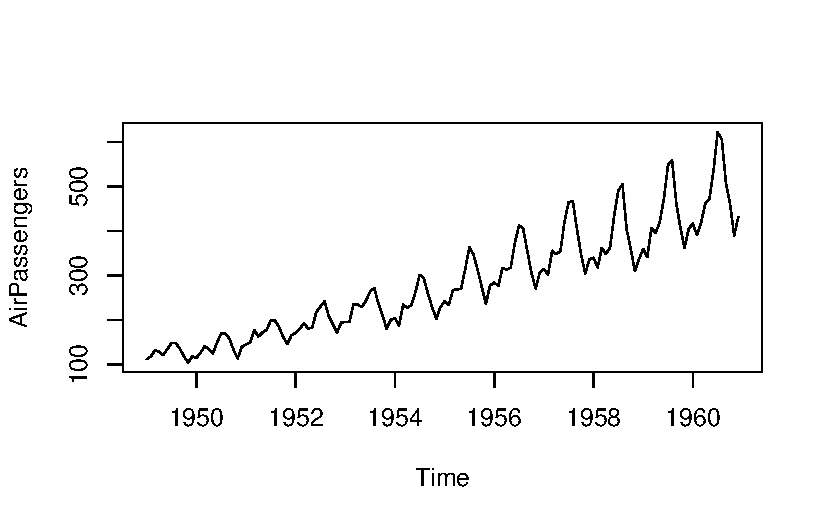
\includegraphics{series_files/figure-pdf/fig-PAP-1.pdf}

}

\subcaption{\label{fig-PAP-1}Datos de AirPassengers.}

\end{minipage}%
%
\begin{minipage}{0.33\linewidth}

\centering{

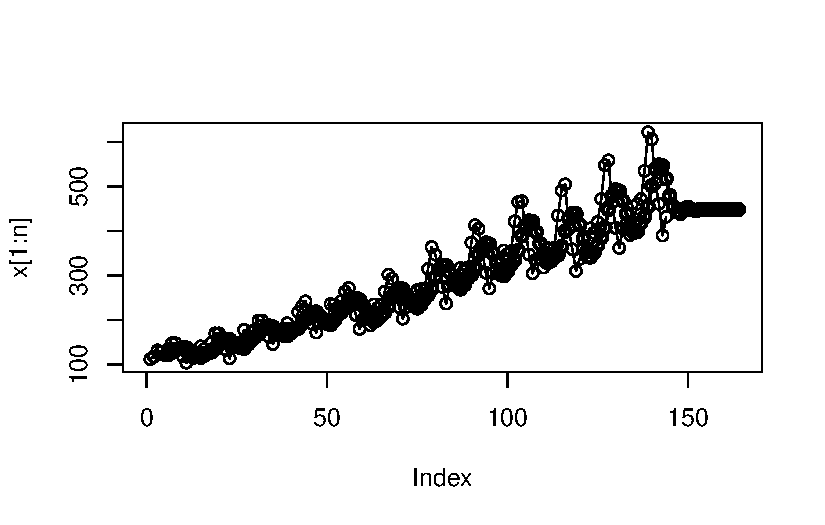
\includegraphics{series_files/figure-pdf/fig-PAP-2.pdf}

}

\subcaption{\label{fig-PAP-2}Predicción de AirPassengers por promedio
móvil.}

\end{minipage}%
%
\begin{minipage}{0.33\linewidth}

\centering{

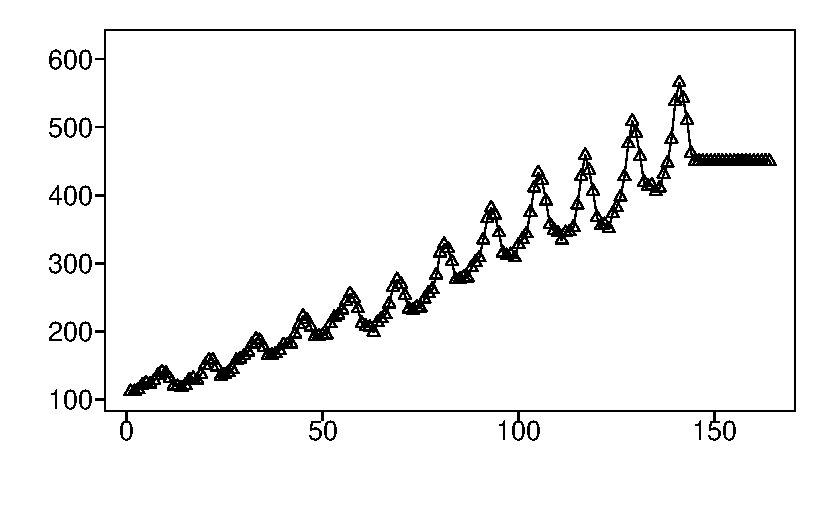
\includegraphics{series_files/figure-pdf/fig-PAP-3.pdf}

}

\subcaption{\label{fig-PAP-3}Predicción de AirPassengers por
suavizamiento exponencial.}

\end{minipage}%

\caption{\label{fig-PAP}Datos de AirPassengers, predicción por promedio
móvil y suavizado exponencial.}

\end{figure}%

\end{tcolorbox}

\end{example}

\subsection{Pronóstico Holt-Winters}\label{pronuxf3stico-holt-winters}

El enfoque Holt-Winters es una técnica desarrollada por los economistas
Holt (1957) y Winters (1960).

Este método de predicción es una extensión del suavizado exponencial y
se aplica a series temporales univariadas. El método no necesita un gran
almacenamiento de datos y es simple. Es adecuado para la predicción a
corto plazo y utiliza la función de máxima verosimilitud para estimar
los parámetros. Existen dos modelos de Holt-Winter que utilizan modelos
aditivos o multiplicativos basados en el componente estacional. Los
modelos aditivos se aplican para un modelo con una tendencia lineal y
con una tendencia exponencial.

\subsubsection{Ecuaciones aditivas de
Holt-Winters}\label{ecuaciones-aditivas-de-holt-winters}

El modelo aditivo de Holt-Winters para datos con tendencia y
estacionalidad que no aumentan con el tiempo es adecuado (consulte la
ecuación (\ref{eq-addseas})). Las fórmulas para la predicción de
Holt-Winters son generalizaciones de las ecuaciones de suavizado
exponencial; y las ecuaciones de Holt-Winters son las siguientes:

\begin{equation}\phantomsection\label{eq-extexp}{
\begin{split}
u_{_t}&= \alpha(x_{_t}-s_{_{t-m}})+(1-\alpha)(u_{_{t-1}}+v_{_{t-1}})\\
v_{_t}&= \beta(u_{_t}-u_{_{t-1}})+(1-\beta)v_{_{t-1}}\\
s_{_t}&= \gamma(x_{_t}-u_{_{t-1}})+(1-\gamma)s_{_{t-m}}
\end{split}
}\end{equation}

Donde \(0 \le \alpha, \beta, \gamma \le 1\), y \(m\) es la longitud del
período (por ejemplo, la frecuencia en un archivo de series temporales).
Para datos mensuales, \(m = 12\), y para datos trimestrales, \(m = 4\).
Los valores \(u_{_t}\) están relacionados con el suavizado exponencial
simple y proporcionan una línea base. Los valores \(v_{_t}\) y
\(s_{_t}\) se relacionan con los efectos de tendencia y estacionales,
respectivamente. Para los tiempos \(t= m+1,\ldots, n\), las predicciones
de un paso adelante, \(\hat{x}_{_t}\), para la media en el tiempo \(t\),
se expresan como:

\[ \hat{x}_{_t}= u_{_{t-1}}+v_{_{t-1}}+s_{_{t-m}}.\]

Las predicciones para \(x_{_{n+l}}, l=1,\ldots,K\) (es decir, hasta
\(K\) pasos más allá del final de los datos observados), se proporcionan
de manera recursiva mediante:

\[
\hat{x}_{_{n+l|n}}=u_{_n}+mv_{_n}+s_{_{n+l-ml'}}.
\]

Donde \(l' =\left[ \frac{l-1}{m} \right] + 1\), con
\(\left[ \frac{l-1}{m} \right]\) denotando el entero mayor o igual a
\(\frac{l-1}{m}\). Aquí, \(\alpha, \beta\) y \(\gamma\) son parámetros
de suavizado, y se pueden obtener utilizando la función
\textbf{HoltWinters} la cual parte de las funciones base que conforman
al software \emph{R}.

\subsubsection{Ecuaciones multiplicativas de
Holt-Winters}\label{ecuaciones-multiplicativas-de-holt-winters}

Como sugiere el término, las ecuaciones multiplicativas de Holt-Winters
son aplicables a datos para los cuales el modelo multiplicativo
(ecuación (\ref{eq-mulseas})) es apropiado. En este caso, las ecuaciones
de Holt-Winters son:

\[
\begin{split}
u_{_t}&= \alpha(x_{_t}/s_{_{t-m}})+(1-\alpha)(u_{_{t-1}}+v_{_{t-1}})\\
v_{_t}&= \beta(u_{_t}-u_{_{t-1}})+(1-\beta)v_{_{t-1}}\\
s_{_t}&= \gamma(x_{_t}/u_{_{t-1}})+(1-\gamma)s_{_{t-m}}
\end{split}
\]

Donde \(0 \le \alpha, \beta, \gamma \le 1\), y donde nuevamente, \(m\)
es la frecuencia. Las predicciones para los valores de \(x_{_t}\) se
expresan mediante:

\[ \hat{x}_{_t}= (u_{_{t-1}}+v_{_{t-1}})s_{_{t-m}} \]

Las predicciones para \(x_{_{n+l}}, l=1,\ldots,K\) (es decir, hasta
\(K\) pasos más allá del final de los datos observados), se proporcionan
de manera recursiva mediante:

\[
\hat{x}_{_{n+l|n}}=(u_{_n}+lv_{_n})s_{_{n+l-ml'.}}
\]

Donde \(l' =\left[ \frac{l-1}{m} \right] + 1\).

\begin{example}[]\protect\hypertarget{exm-HWAP}{}\label{exm-HWAP}

~

\begin{tcolorbox}[enhanced jigsaw, breakable, colbacktitle=quarto-callout-caution-color!10!white, rightrule=.15mm, toptitle=1mm, colback=white, left=2mm, colframe=quarto-callout-caution-color-frame, bottomtitle=1mm, opacitybacktitle=0.6, leftrule=.75mm, arc=.35mm, title={AirPassengers}, coltitle=black, titlerule=0mm, opacityback=0, bottomrule=.15mm, toprule=.15mm]

Reconsidere los datos de AirPassengers. Dado que los puntos temporales
posteriores revelan magnitudes crecientes de los picos y valles
cíclicos, la serie temporal es multiplicativa en lugar de aditiva. La
Figura~\ref{fig-HWAP-1} muestra las predicciones de un paso adelante de
Holt-Winters para los años 1950-1960 (superpuestas a los datos reales)
dadas por la fórmula utilizando los parámetros de suavizado y
coeficientes estimados anteriormente. Las predicciones de un paso
adelante (línea sólida) son bastante precisas y apenas se distinguen de
los datos (puntos en la línea). La Figura~\ref{fig-HWAP-2} muestra los
datos de AirPassengers junto con las predicciones de Holt-Winters para
los próximos tres años (línea punteada). Estas predicciones parecen
extender con precisión el patrón precedente.

\begin{Shaded}
\begin{Highlighting}[]
\CommentTok{\# Figure 2.20(a)}
\NormalTok{ap.hw}\OtherTok{=}\FunctionTok{HoltWinters}\NormalTok{(AirPassengers,}\AttributeTok{seasonal=}\StringTok{"mult"}\NormalTok{)}
\FunctionTok{plot}\NormalTok{(ap.hw)}
\CommentTok{\# Figure 2.20(b)}
\NormalTok{ap.pred}\OtherTok{=}\FunctionTok{predict}\NormalTok{(ap.hw,}\AttributeTok{n.ahead=}\DecValTok{36}\NormalTok{)}
\FunctionTok{plot}\NormalTok{(ap.hw,ap.pred,}\AttributeTok{lty=}\DecValTok{1}\SpecialCharTok{:}\DecValTok{2}\NormalTok{)}
\end{Highlighting}
\end{Shaded}

\begin{figure}[H]

\begin{minipage}{0.50\linewidth}

\centering{

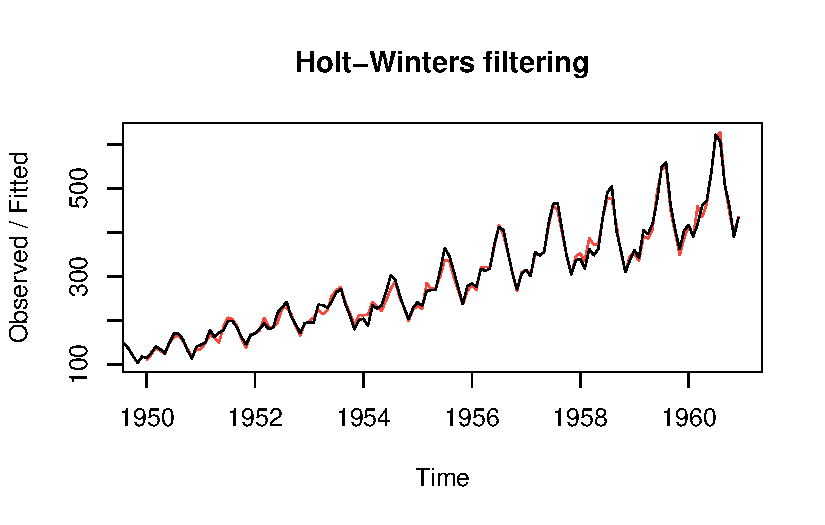
\includegraphics{series_files/figure-pdf/fig-HWAP-1.pdf}

}

\subcaption{\label{fig-HWAP-1}Predicción de AirPassengers un paso
adelante}

\end{minipage}%
%
\begin{minipage}{0.50\linewidth}

\centering{

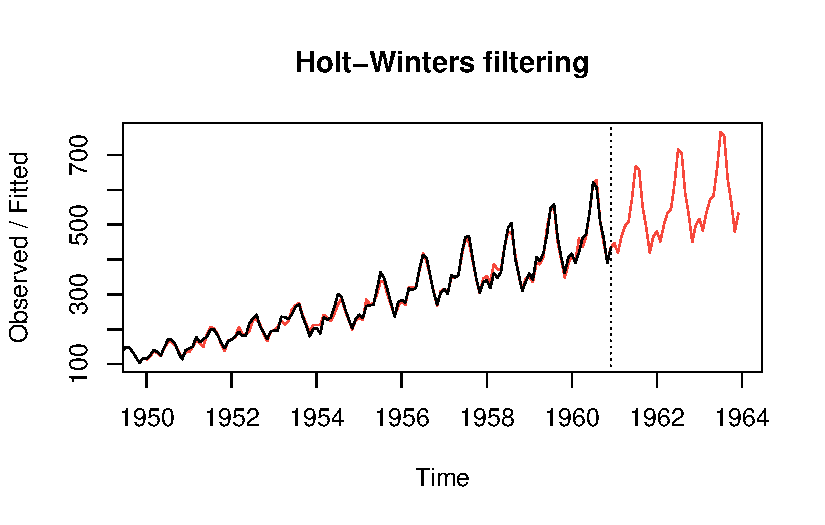
\includegraphics{series_files/figure-pdf/fig-HWAP-2.pdf}

}

\subcaption{\label{fig-HWAP-2}Predicción por Holt-Winters de
AirPassengers}

\end{minipage}%

\caption{\label{fig-HWAP}Predicción mediante Holt-Winters de los datos
de AirPassengers.}

\end{figure}%

\end{tcolorbox}

\end{example}

\subsection{Modelo Autoregresivo (AR)}\label{modelo-autoregresivo-ar}

\begin{definition}[]\protect\hypertarget{def-mARp}{}\label{def-mARp}

Se afirma que el proceso \(X_{_t}\) satisface un modelo
\(\mathrm{AR}(p)\) (Autoregresivo de orden \(p\)) si

\begin{equation}\phantomsection\label{eq-ARp}{
X_{_t}=a_{_t}+\beta+\sum_{k=1}^p \phi_{_k}X_{_{t-k}},
}\end{equation}

donde \(\phi_{_k}, k=1,\ldots,p\) son constantes reales,
\(\beta = \left(1-\phi_{_1}-\phi_{_2}-\cdots-\phi_{_p}\right)\mu\),
\(\phi_{_p}\neq 0\), y \(a_{_t}\) es un proceso de ruido blanco con
media cero y varianza finita \(\sigma_{_a}^2\).

\end{definition}

La fórmula en la ecuación (\ref{eq-ARp}) indica que, el valor del
proceso en el tiempo \(t\), es una combinación lineal de los \(p\)
valores anteriores más un componente de ruido aleatorio en \(a_{_t}\).
Iniciamos nuestra discusión sobre los modelos \(\mathrm{AR}\) al abordar
sus propiedades, incluidas las condiciones de estacionariedad y el
comportamiento de las autocorrelaciones y densidades espectrales para
modelos específicos.

El modelo \(\mathrm{AR}(p)\) general definido en la
Definición~\ref{def-mARp}, se asemeja a una ecuación de regresión
múltiple, donde, en este caso, las ``variables independientes'' son los
\(p\) valores previos de la ``variable dependiente'' \(X_{_t}\). Otra
forma de escribir la ecuación (\ref{eq-ARp}), después de reorganizar los
términos, es:

\begin{equation}\phantomsection\label{eq-oarp}{
X_{_t}-\mu-\phi_{_1}(X_{_{t-1}}-\mu)-\phi_{_2}(X_{_{t-2}}-\mu)-\cdots-\phi_{_p}(X_{_{t-p}}-\mu)=a_{_t}.
}\end{equation}

Al igual que en el caso de los modelos \(\mathrm{AR}(1)\) y
\(\mathrm{AR}(2)\), se expresará con frecuencia el \(\mathrm{AR}(p)\) en
la forma de media cero:

\begin{equation}\phantomsection\label{eq-m0arp}{
X_{_t} -\phi_{_1}X_{_{t-1}}-\phi_{_2}X_{_{t-2}}-\cdots-\phi_{_p}X_{_{t-p}}=a_{_t}.
}\end{equation}

Las ecuaciones (\ref{eq-ARp}) a (\ref{eq-m0arp}) dan la impresión de que
un modelo \(\mathrm{AR}(p)\) será mucho más complicado de manejar que un
modelo \(\mathrm{AR}(1)\) o \(\mathrm{AR}(2)\). La comprensión de las
características de los modelos \(\mathrm{AR}(1)\) y \(\mathrm{AR}(2)\)
conduce directamente a comprender el comportamiento de un modelo
\(\mathrm{AR}(p)\).

\paragraph{\texorpdfstring{Hechos sobre el modelo
\(\mathrm{AR}(p)\)}{Hechos sobre el modelo \textbackslash mathrm\{AR\}(p)}}\label{hechos-sobre-el-modelo-mathrmarp}

\begin{enumerate}
\def\labelenumi{\roman{enumi}.}
\item
  \(\mathrm{E}[X_{_t}]=\mu\), para la forma ``no nula de la media'' del
  modelo \(\mathrm{AR}(p)\) en la (\ref{eq-oarp}) y (\ref{eq-m0arp}).
\item
  El proceso de varianza es
  \[\sigma_{_X}^2=\gamma_{_0}=\frac{\sigma_{_a}^2}{1-\phi_{_1}\rho_{_1}-\phi_{_2}\rho_{_2}-\cdots-\phi_{_p}\rho_{_p}},\]

  la cuál es contante y finita cuando \(X_{_t}\) es estacionaria.
\item
  La autocorrelación de un proceso \(\mathrm{AR}(p)\) satisface
  \begin{equation}\phantomsection\label{eq-autoarp}{
  \rho_{_k}=\phi_{_p}+\sum_{n=1}^{p-1}\phi_{_n}\rho_{_{k-n}}.
  }\end{equation}

  La ecuación (\ref{eq-autoarp}) conduce a las ecuaciones de Yule-Walker
  de orden \(p\times p\): \[
      \begin{split}
  \rho_{_{1}} &= \phi_{_1}+\phi_{_{2}} \rho_{_1} +\ldots + \phi_{_p} \rho_{_{p-1}} \\
  \rho_{_{2}} &= \phi_{_1}\rho_{_1}+\phi_{_{2}}  +\ldots + \phi_{_p} \rho_{_{p-2}}\\
  &\vdots \\
  \rho_{_{p}} &= \phi_{_1}\rho_{_{p-1}}+\phi_{_{2}} \rho_{_{p-2}} +\ldots + \phi_{_p}.
  \end{split}
    \]

  Conocer los valores de \(\phi_{_1}, \phi_{_2}, \ldots, \phi_{_p}\) nos
  permite resolver este sistema de ecuaciones de dimensión \(p\times p\)
  para \(\rho_{_k}\), donde \(k = 1, 2, \ldots, p\). Las
  autocorrelaciones basadas en el modelo, \(\rho_{_k}\), para \(k > p\),
  se pueden calcular utilizando la recursión
  \(\phi_{_1} \rho_{_{k-1}} - \phi_{_2} \rho_{_{k-2}} + \ldots + \phi_{_p} \rho_{_{k-p}}\).
  No sorprendentemente, se utilizan funciones computacionales para
  realizar estos cálculos.
\item
  La densidad espectral de un modelo \(\mathrm{AR}(p)\) es dada por

  \[
  S_{_X}(f)=\frac{\sigma_{_a}^2}{\gamma_{_0}|1-\phi_{_1}e^{-2\pi i f}-\phi_{_2}e^{-4\pi i f}-\cdots-\phi_{_p}e^{-2p\pi i f}|^2}
  \]
\end{enumerate}

\begin{definition}[Autocorrelaciones
parciales]\protect\hypertarget{def-pac}{}\label{def-pac}

Sea \(X_{_t}\) un proceso estacionario con autocorrelaciones
\(\rho_{_j}=j=0,1,\ldots\).

\begin{enumerate}
\def\labelenumi{\alph{enumi}.}
\item
  La autocorrelación parcial en rezago \(k\), denotada como
  \(\phi_{_{kk}}\) , es la correlación entre \(X_{_t}\) y
  \(X_{_{t+ k}}\) condicional al ``conocimiento'' de las variables
  intervinientes \(X_{_{t+1}}, X_{_{t+2}}\), y \(X_{_{t+k-1}}\).
\item
  Considere las siguientes ecuaciones de Yule-Walker donde
  \(\phi_{_{kj}}\) denota el coeficiente \(j-\)ésimo asociado con las
  ecuaciones de Yule-Walker de orden \(k\).

  \[\begin{split} k&=1\\ \rho_{_1}&=\phi_{_{11}}\\ \\ k&=2\\ \rho_{_1}&=\phi_{_{21}}+\phi_{_{22}}\rho_{_1}\\ \rho_{_2}&=\phi_{_{21}}\rho_{_1}+\phi_{_{22}}\end{split}\]

  En general\ldots{}

  \[\begin{split}\rho_{_1}&=\phi_{_{k1}}+\phi_{_{k2}}\rho_{_1}+\cdots+\phi_{_{kk}}\rho_{_{k-1}}\\\rho_{_2}&=\phi_{_{k1}}\rho_{_1}+\phi_{_{k2}}+\cdots+\phi_{_{kk}}\rho_{_{k-2}}\\ \vdots\\ \rho_{_k}&=\phi_{_{k1}}\rho_{_{k-1}}+\phi_{_{k2}}\rho_{_{k-2}}+\cdots+\phi_{_{kk}}\end{split}\]

  La función de autocorrelación parcial se define como
  \(\phi_{_{kk}}, k = 1, 2,...\).
\end{enumerate}

\end{definition}

\paragraph{\texorpdfstring{Notación de operador y ecuación
característica para un
\(\mathrm{AR}(p)\)}{Notación de operador y ecuación característica para un \textbackslash mathrm\{AR\}(p)}}\label{notaciuxf3n-de-operador-y-ecuaciuxf3n-caracteruxedstica-para-un-mathrmarp}

El modelo \(\mathrm{AR}(p)\) en la ecuación (\ref{eq-oarp}) puede ser
escrito en notación de operador como

\[
(1-\phi_{_1}B-\phi_{_2}B^2-\cdots-\phi_{_p}B^p)(X_{_t}-\mu)=a_{_t}.
\]

También puede ser escrito utilizando la notación,
\(\phi(B)(X_{t}-\mu)=a_{_t}\) , donde \(\phi(B)\) es el operador de
orden \(p\)

\[
\phi(B)=1-\phi_{_1}B-\phi_{_2}B^2-\cdots-\phi_{_p}B^p.
\]

Convirtiendo el operador \(\phi(B)\) en la expresión algebraica
\(\phi(z)\) resulta en el polinomio característico general
\(\mathrm{AR}(p)\)

\[
\phi(z)=1-\phi_{_1}z-\phi_{_2}z^2-\cdots-\phi_{_p}z^p.
\]

La correspondiente ecuación característica \(\mathrm{AR}(p)\) es

\[\phi(z) = 1 -\phi_{_1}z -\phi_{_2}z^2 - \cdots - -\phi_{_p}z^p = 0.\]

La ecuación característica tiene \(p\) raíces
\(r_{_1}, r_{_2} ,\ldots, r_{_p}\) que son reales y/o complejas, donde
las raíces complejas aparecen como pares conjugados y algunas raíces
pueden ser repetidas.

\begin{theorem}[]\protect\hypertarget{thm-arpest}{}\label{thm-arpest}

Un proceso \(\mathrm{AR}(p)\) es estacionario si y solo si todas las
raíces de la ecuación característica son mayores que uno en valor
absoluto.

\begin{proof}
Vea Harvey (1981).
\end{proof}

\end{theorem}

\begin{example}[]\protect\hypertarget{exm-ar4}{}\label{exm-ar4}

~

\begin{tcolorbox}[enhanced jigsaw, breakable, colbacktitle=quarto-callout-caution-color!10!white, rightrule=.15mm, toptitle=1mm, colback=white, left=2mm, colframe=quarto-callout-caution-color-frame, bottomtitle=1mm, opacitybacktitle=0.6, leftrule=.75mm, arc=.35mm, title={Un modelo \(\mathrm{AR}(4)\)}, coltitle=black, titlerule=0mm, opacityback=0, bottomrule=.15mm, toprule=.15mm]

Considere el modelo \(\mathrm{AR}(4)\)

\begin{equation}\phantomsection\label{eq-ejar4}{
X_{_t}-0.13X_{_{t-1}}-1.4414X_{_{t-2}}+.0326X_{_{t-3}}+.8865X_{_{t-4}}=a_{_{t}}
}\end{equation}

en el que \(\sigma_{_a}^2 = 1\). La notación del operador para este
modelo es

\[ (1 - 0.13B + 1.4414B^2 - .0326B^3 + 0.8865 B^4)X_{_t}= a_{_t},\]

donde la correspondiente ecuación característica es

\[1 - 0.13z + 1.4414z^2 - .0326z^3 + 0.8865 z^4 = 0.\]

La Figura~\ref{fig-ejar4} representa una realización de longitud
\(n = 200\) del proceso descrito en la ecuación (\ref{eq-ejar4}), junto
con las autocorrelaciones muestrales asociadas y la estimación de la
densidad espectral Parzen, respectivamente.

\begin{Shaded}
\begin{Highlighting}[]
\FunctionTok{library}\NormalTok{(tswge)}
\NormalTok{x}\OtherTok{=}\FunctionTok{gen.arma.wge}\NormalTok{(}\AttributeTok{n=}\DecValTok{200}\NormalTok{,}\AttributeTok{phi=}\FunctionTok{c}\NormalTok{(}\FloatTok{0.1300}\NormalTok{,}\FloatTok{1.4414}\NormalTok{,}\SpecialCharTok{{-}}\NormalTok{.}\DecValTok{0326}\NormalTok{,}\SpecialCharTok{{-}}\NormalTok{.}\DecValTok{8865}\NormalTok{),}\AttributeTok{sn=}\DecValTok{9310}\NormalTok{,}\AttributeTok{plot=}\ConstantTok{FALSE}\NormalTok{)}
\FunctionTok{plotts.sample.wge}\NormalTok{(x)}
\end{Highlighting}
\end{Shaded}

\begin{figure}[H]

\centering{

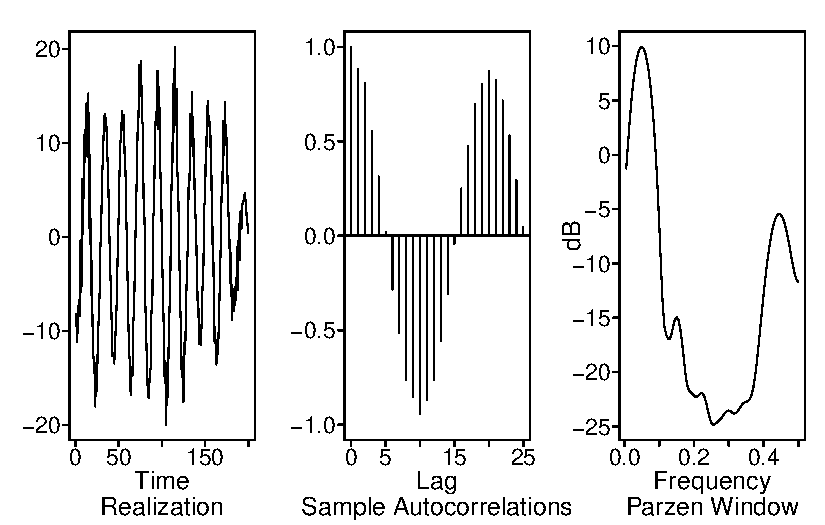
\includegraphics{series_files/figure-pdf/fig-ejar4-1.pdf}

}

\caption{\label{fig-ejar4}Realización del modelo AR(4).}

\end{figure}%

\end{tcolorbox}

\end{example}

\paragraph{El Test Aumentado de
Dickey-Fuller}\label{el-test-aumentado-de-dickey-fuller}

Este test ha estado en uso durante muchos años para probar las
hipótesis:

\begin{itemize}
\item
  \(H_{_0}:\) el modelo contiene una raíz unitaria.
\item
  \(H_{_a}\): el modelo no contiene una raíz unitaria (y por lo tanto es
  estacionario).
\end{itemize}

Estadístico de prueba: \(\uptau\)

Región de rechazo: Rechazar \(H_{_0}\) si \(\uptau < d_{_\alpha}\),
donde \(d_{_\alpha}\) es el valor crítico de nivel \(\alpha\).

David Alan Dickey (1976) obtiene la distribución límite (complicada) del
estadístico de prueba. Si \(\uptau \geq d_{_{.05}}\), entonces no se
rechaza \(H_{_0}\) y la prueba de Dickey-Fuller detecta una raíz
unitaria. Nótese que, el rechazo de la hipótesis nula, lleva a la
conclusión de que el proceso es estacionario. Por lo tanto, la
conclusión de una raíz unitaria se basa en no rechazar la hipótesis
nula. Es importante recalcar que no rechazar la hipótesis nula no
implica creer que la hipótesis nula sea verdadera, sino simplemente que
no hubo suficiente evidencia para rechazarla.

Para llevar a cabo pruebas de raíz unitaria, se empleará una
implementación del test del software estadístico R. Existen diversas
opciones, y se utilizará el siguiente comando que incorpora una
constante pero no una tendencia en el modelo, y utiliza el criterio de
información de Akaike (AIC) para seleccionar el número de rezagos. Se
recomienda consultar las obras de David A. Dickey y Fuller (1979) o
Fuller (1995) para obtener más detalles al respecto.

\paragraph{\texorpdfstring{Factorización del polinomio característico de
un
\(\mathrm{AR}(p)\)}{Factorización del polinomio característico de un \textbackslash mathrm\{AR\}(p)}}\label{factorizaciuxf3n-del-polinomio-caracteruxedstico-de-un-mathrmarp}

Las raíces de una ecuación cuadrática se pueden encontrar mediante el
uso de la fórmula cuadrática. Sin embargo, las cosas se vuelven más
complicadas para órdenes polinómicos mayores a dos. La ecuación cúbica

\[
1-2.1z+1.6z^2-.3z^3=0
\]

puede factorizarse en la forma \((1-.5z)(1-1.6z+.8z^2)\). Basándose en
esta factorización, las raíces que se obtienen son \(r_{_1} = 1/.5=2\),
\(r_{_2} = 1+.5i\) y \(r_{_3} = 1-.5i\). Es decir, este
\(\mathrm{AR}(3)\) tendrá un comportamiento de primer orden asociado con
\(1-.5B\) (es decir, una frecuencia de cero), un comportamiento cíclico
de segundo orden con una frecuencia de sistema \(f_{_0} = 0.07\), y el
proceso es estacionario porque todas las raíces están fuera del círculo
unitario.

\begin{theorem}[]\protect\hypertarget{thm-poli}{}\label{thm-poli}

El polinomio de orden \(p\),
\(1-\phi_{_1}z-\phi_{_2}z^2-\cdots-\phi_{_p}z^p\), siempre puede
descomponerse como un producto de

\begin{enumerate}
\def\labelenumi{\roman{enumi}.}
\item
  Factores de primer orden (lineales) asociados con raíces reales.
\item
  Factores de segundo orden (cuadráticos) cuyas raíces son pares
  conjugados complejos.
\end{enumerate}

\end{theorem}

\paragraph{\texorpdfstring{Tablas de factores para modelos
\(\mathrm{AR}(p)\)}{Tablas de factores para modelos \textbackslash mathrm\{AR\}(p)}}\label{tablas-de-factores-para-modelos-mathrmarp}

El Teorema~\ref{thm-poli} establece que, cualquier polinomio de orden
\(p\) puede expresarse como un producto de factores de primer orden y/o
factores irreducibles de segundo orden. Comprender los factores de
primer y segundo orden es la clave para comprender el modelo
\(\mathrm{AR}(p)\).

\begin{tcolorbox}[enhanced jigsaw, breakable, colbacktitle=quarto-callout-caution-color!10!white, rightrule=.15mm, toptitle=1mm, colback=white, left=2mm, colframe=quarto-callout-caution-color-frame, bottomtitle=1mm, opacitybacktitle=0.6, leftrule=.75mm, arc=.35mm, title={Ejemplo~\ref{exm-ar4} (Continuación\ldots)}, coltitle=black, titlerule=0mm, opacityback=0, bottomrule=.15mm, toprule=.15mm]

Se considera de nuevo el modelo \(\mathrm{AR}(4)\) descrito en la
ecuación (\ref{eq-ejar4}). La ecuación característica asociada es

\[
1-.13z-1.4414z^2+.0326z^3+.8865z^4=0.
\]

La forma factorizada (obtenida numéricamente) es

\[
(1-1.89B+.985B^2)(1+1.76B+.9B^2)=0.
\]

La tabla de factores es una herramienta muy útil para resumir
rápidamente la escencia de un modelo \(\mathrm{AR}(p)\) con respecto a
los factores de primer y segundo orden.

\begin{Shaded}
\begin{Highlighting}[]
\FunctionTok{library}\NormalTok{(tswge)}
\FunctionTok{factor.wge}\NormalTok{(}\AttributeTok{phi=}\FunctionTok{c}\NormalTok{(.}\DecValTok{13}\NormalTok{,}\FloatTok{1.4414}\NormalTok{,}\SpecialCharTok{{-}}\NormalTok{.}\DecValTok{0326}\NormalTok{,}\SpecialCharTok{{-}}\NormalTok{.}\DecValTok{8865}\NormalTok{))}
\end{Highlighting}
\end{Shaded}

\begin{verbatim}
  
  
Coefficients of AR polynomial:  
0.1300 1.4414 -0.0326 -0.8865 

                           AR Factor Table 
Factor                 Roots                Abs Recip    System Freq 
1-1.8900B+0.9850B^2    0.9594+-0.3079i      0.9925       0.0494
1+1.7600B+0.9000B^2   -0.9778+-0.3938i      0.9487       0.4391
  
  
\end{verbatim}

En este caso, hay dos factores de segundo orden, \(1-1.89B+.985B^2\) y
\(1+1.76B+.9B^2\).

\end{tcolorbox}

\section{Evaluación de la precisión de los
pronósticos}\label{evaluaciuxf3n-de-la-precisiuxf3n-de-los-pronuxf3sticos}

Para obtener una cuantificación ``general'' de la calidad de las
predicciones, se evalúa qué tan bien coinciden las predicciones
(\(f_{_t}\)) con los valores reales (\(y_{_t}\)) en el tiempo \(t\).
Afortunadamente, se han ideado métricas de error para evaluar la calidad
del modelo y permitir la comparación con otras regresiones que poseen
diferentes parámetros. Estas métricas son resúmenes breves pero
informativos de la calidad de los datos. A continuación se presentan
algunas métricas de rendimiento más comunes (Segall y Niu (2022)).

\subsection{MAE}\label{mae}

El error absoluto medio (MAE) se calcula tomando el residuo para cada
punto de datos, considerando únicamente el valor absoluto para minimizar
el impacto de los valores atípicos en comparación con la ecuación
(\ref{eq-RMSE}). Luego, se obtiene el promedio de todos estos residuos.
La ecuación formal se presenta a continuación:
\begin{equation}\phantomsection\label{eq-MAE}{MAE= \frac{1}{n}\sum_{t=1}^n |y_{_t}-f_{_t}|.}\end{equation}
Dado que se emplea el valor absoluto del residuo, no se indica el
rendimiento inferior o superior del modelo. Cada residuo contribuye de
manera equitativa al error total, y los errores más grandes tienen una
mayor contribución al error general. Un MAE pequeño indica un buen
rendimiento de predicción, mientras que un MAE grande sugiere que el
modelo puede tener dificultades en ciertas áreas. Obtener MAE perfecta
de 0 es rara, indica que el modelo es un predictor impecable.

Sin embargo, el uso del valor absoluto del residuo puede no ser el mejor
enfoque para interpretar los datos, ya que los \emph{valores atípicos}
(es decir, los puntos de datos que se alejan significativamente de la
tendencia general de los datos) pueden afectar significativamente el
rendimiento del modelo. Dependiendo del tratamiento de los valores
atípicos y extremos en los datos, es posible que se desee resaltar o
minimizar su impacto. Como resultado, la elección de la métrica de error
adecuada puede verse influida por el problema de los valores atípicos.

\subsection{MSE}\label{mse}

El error cuadrático medio (MSE) es similar al MAE, pero eleva al
cuadrado la diferencia antes de sumarlos todos en lugar de utilizar el
valor absoluto. Esta diferencia se puede observar en la siguiente
ecuación:
\begin{equation}\phantomsection\label{eq-MSE}{MSE=\frac{1}{n} \sum_{t=1}^n (y_{_t}-f_{_t})^2.}\end{equation}
El error medio absoluto (MAE) y el error cuadrático medio (MSE) son
métricas de error comúnmente utilizadas en la evaluación de modelos. Sin
embargo, el MSE suele ser mayor que el MAE debido al cuadrado de la
diferencia. Comparar los dos directamente no siempre es posible, y en su
lugar, debemos comparar las métricas de error de nuestro modelo con las
de un modelo ya conocido o que se ajuste a la serie de datos. El efecto
de los valores atípicos en nuestros datos es más evidente con la
presencia del término cuadrado en la ecuación MSE. Mientras que cada
residuo en MAE contribuye proporcionalmente al error total, el error
crece cuadráticamente en MSE. En última instancia, esto significa que
los valores atípicos en nuestros datos contribuirán a un error total
mucho mayor en el MSE que en el MAE. Del mismo modo, nuestro modelo se
verá más penalizado por hacer predicciones que difieran mucho del valor
real correspondiente.

\subsection{RMSE}\label{rmse}

RMSE, o error cuadrático medio, es una medida frecuentemente utilizada
para evaluar la diferencia entre los valores predichos \(f_{_t}\) y los
valores observados \(y_{_t}\). Su función se expresa a continuación,
donde \(n\) representa el número de observaciones. En comparación con el
error cuadrático medio (MSE), RMSE toma la raíz cuadrada de MSE y
restituye la unidad al mismo nivel que la variable dependiente. Por lo
tanto, tiene la ventaja de ser interpretado directamente. En general, un
valor de RMSE más bajo es preferible, y RMSE\(=0\) indica un ajuste
perfecto de los datos. La desventaja de RMSE es su sensibilidad a
valores atípicos, ya que unos pocos errores grandes en la suma pueden
generar un aumento significativo, y la prueba no distingue entre
subestimación y sobreestimación. Como se discutió anteriormente en la
descripción de los datos, el conjunto de datos que se utiliza tiene
varios valores extremos de gastos elevados, por lo que utilizar solo
RMSE como medida podría no ser muy adecuado.

La fórmula para el cálculo de RMSE es la siguiente:
\begin{equation}\phantomsection\label{eq-RMSE}{RMSE= \sqrt{\frac{\sum_{t=1}^n (y_t-f_t)^2}{n}}.}\end{equation}

\subsection{MAPE}\label{mape}

El error porcentual absoluto medio (MAPE) mide la precisión de la
predicción como un porcentaje y se define generalmente de la siguiente
manera.
\begin{equation}\phantomsection\label{eq-MAPE}{MAPE=\frac{100}{n}\sum_{t=1}^n \left| \frac{y_t-f_t}{y_t}\right|.}\end{equation}

La ventaja es que es muy intuitivo interpretar el error relativo, y un
MAPE más bajo significa un error menor. MAPE es similar a MAE, pero
normaliza MAE mediante observaciones reales, resolviendo así el problema
de que MAE proporciona poca información sobre el error al comparar datos
de diferentes escalas. Sin embargo, también presenta la desventaja de
que puede producir valores infinitos o indefinidos para valores reales
cercanos o iguales a cero. Otra limitación de MAPE es que penaliza más
los errores negativos que los errores positivos. Por ejemplo, para un
valor real de \(100\) y un valor estimado de \(90\), el MAPE es
\(0.10\). Para el mismo valor estimado y un valor real de \(80\), el
MAPE es \(0.125\). Como resultado, si se utiliza MAPE como función
objetivo, el estimador preferirá valores más pequeños y puede sesgarse
hacia errores negativos.

\part{Redes neuronales}

\chapter{Redes Neuronales}\label{redes-neuronales-1}

El funcionamiento de los cerebros de humanos y otros animales es
intrigante porque son capaces de realizar tareas muy complejas en un
tiempo muy corto y con alta eficiencia. Por ejemplo, las señales de los
sensores en el cuerpo transmiten información relacionada con la vista,
el oído, el gusto, el olfato, el tacto, el equilibrio, la temperatura,
el dolor, etc. Luego, las neuronas del cerebro, que son unidades
autónomas, transmiten, procesan y almacenan esta información para que se
pueda responder con éxito a estímulos externos e internos. Las neuronas
de muchos animales transmiten picos de actividad eléctrica a través de
una hebra larga y delgada llamada axón. Un axón se divide en miles de
terminales o ramas, donde, según el tamaño de la señal, se conectan a
dendritas de otras neuronas (Figura~\ref{fig-neubio}). Se estima que el
cerebro está compuesto por alrededor de \(10^{11}\) neuronas que
trabajan en paralelo, ya que el procesamiento realizado por las neuronas
y la memoria capturada por las sinapsis se distribuyen juntas sobre la
red. La cantidad de información procesada y almacenada depende de los
niveles umbral de disparo y también del peso dado por cada neurona a
cada una de sus entradas. Una de las características de las neuronas
biológicas, a las que deben su gran capacidad para procesar y realizar
tareas altamente complejas, es que están altamente conectadas con otras
neuronas de las cuales reciben estímulos de un evento a medida que
ocurre, o cientos de señales eléctricas con la información aprendida.

Las redes neuronales tienen sus raíces en la búsqueda de emular el
funcionamiento del cerebro humano en la década de 1940. McCulloch y
Pitts (1943) propusieron el concepto inicial de una ``neurona
artificial'' que podría realizar operaciones lógicas básicas. Sin
embargo, fue en la década de 1950 cuando el psicólogo Frank Rosenblatt
desarrolló el ``perceptrón'', Rosenblatt (1960), un tipo de red neuronal
que podía aprender a reconocer patrones a través de entrenamiento.

A pesar de su potencial, las limitaciones del perceptrón y la falta de
avances en la capacidad computacional llevaron a un declive en la
investigación en redes neuronales en los años siguientes. Sin embargo,
en la década de 1980 y 1990, hubo un resurgimiento del interés debido a
nuevos algoritmos de aprendizaje y avances en el hardware, permitiendo
el entrenamiento de redes más complejas.

La importancia de las redes neuronales en la predicción de datos radica
en su capacidad para aprender patrones y relaciones en conjuntos de
datos vastos y complejos. A través del proceso de entrenamiento, una red
neuronal ajusta sus pesos y conexiones internas para capturar
características relevantes en los datos. Esto les permite realizar
tareas como clasificación y regresión, lo que a su vez permite la
predicción de resultados futuros.

Con el tiempo, las redes neuronales se han vuelto más sofisticadas,
dando lugar a arquitecturas como las redes neuronales convolucionales
(CNN) para el procesamiento de imágenes y las redes neuronales
recurrentes (RNN) para el procesamiento de secuencias. Además, el
surgimiento del aprendizaje profundo (deep learning) ha permitido el
entrenamiento de redes neuronales con muchas capas, lo que ha mejorado
significativamente su capacidad para abordar problemas complejos de
predicción.

\begin{figure}

\centering{

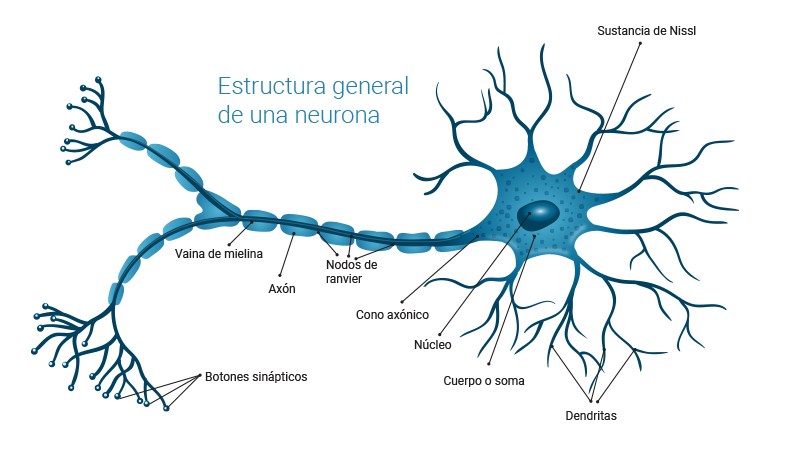
\includegraphics[width=6.52083in,height=\textheight]{Imagenes/rna.png}

}

\caption{\label{fig-neubio}Representación gráfica de una neurona
biológica.}

\end{figure}%

\section{Elementos fundamentales de las Redes Neuronales
Artificiales}\label{elementos-fundamentales-de-las-redes-neuronales-artificiales}

Para obtener una comprensión clara de los principales elementos
utilizados para construir modelos de redes neuronales artificiales
(RNA), en la Figura~\ref{fig-modelogen} se presenta un modelo general de
red neuronal artificial que incorpora los componentes fundamentales para
este tipo de modelos.

\begin{figure}

\centering{

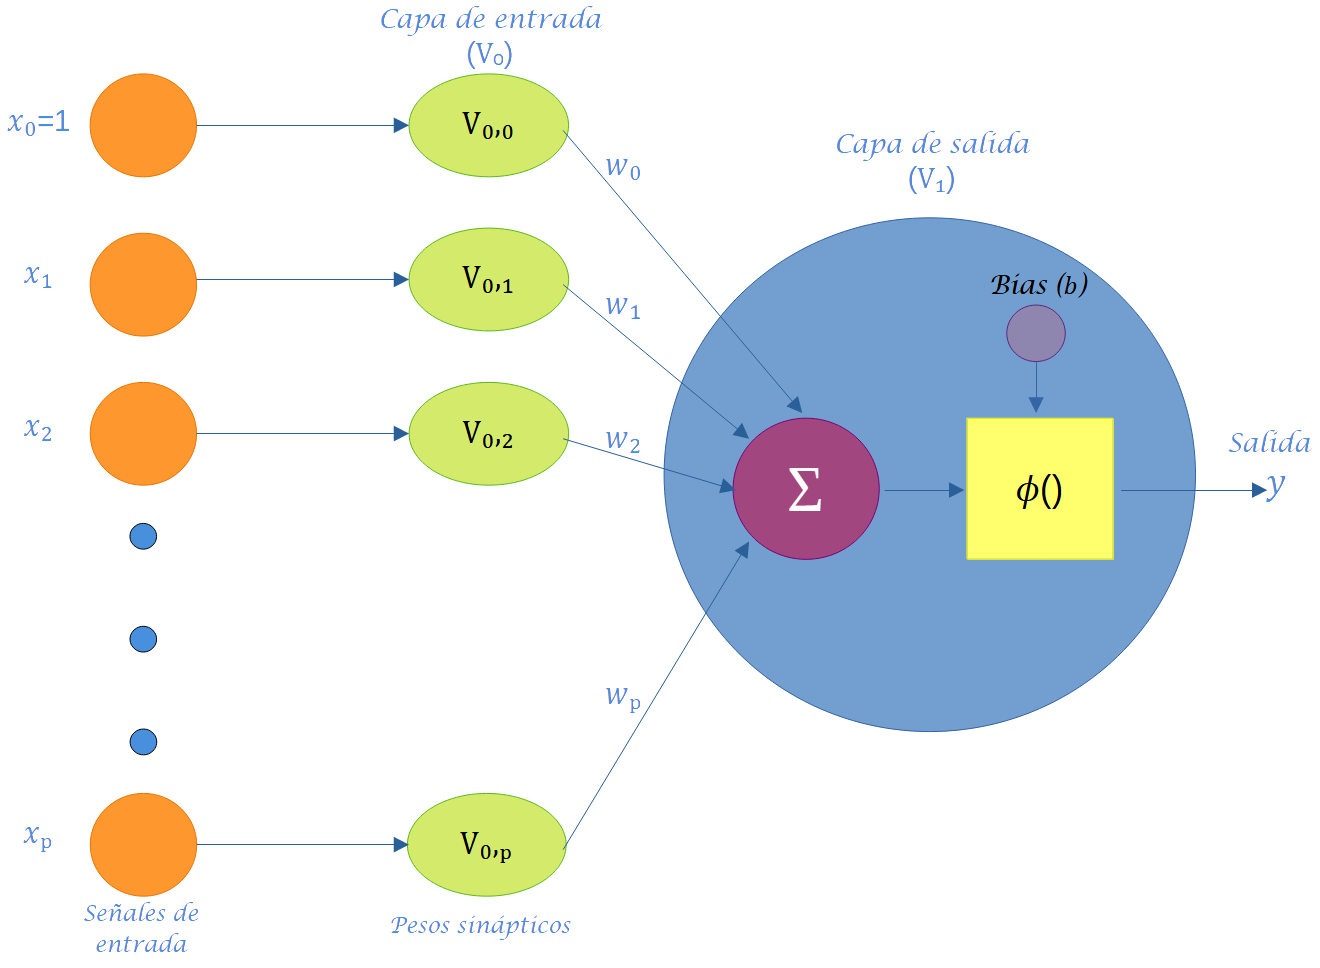
\includegraphics{Imagenes/modgen.png}

}

\caption{\label{fig-modelogen}Modelo general de redes neuronales
artificiales.}

\end{figure}%

La información de entrada, \(x_1, ..., x_p\), es recibida por la neurona
del sistema sensorial externo u otras neuronas con las que tiene
conexión. El vector de pesos sinápticos \(\mathbf{w} = (w_1, ..., w_p)\)
modifica la información recibida emulando la sinapsis entre las neuronas
biológicas. Estos pueden interpretarse como ganancias que pueden atenuar
o amplificar los valores que desean propagar hacia la neurona. El
parámetro \(b_j\) se conoce como el sesgo (intercepto o umbral) de una
neurona. En redes neuronales artificiales, el aprendizaje se refiere al
método de modificar los pesos de las conexiones entre los nodos
(neuronas) de una red especificada.

Los valores recibidos por la neurona son ajustados por los pesos
sinápticos y sumados para generar la entrada neta, expresada
matemáticamente como:

\[v_j=\sum_{j=1}^p \omega_{ij}x_j.\]

La entrada neta \((v_j)\) determina si la neurona se activa o no. La
activación de la neurona depende de la función de activación,
evaluándose la entrada neta en dicha función para obtener la salida de
la red;

\[
y_j=g(v_j),
\]

donde \(g\) representa la función de activación. Por ejemplo, si se
define esta función como un escalón unitario (también llamado umbral),
la salida será \(1\) si la entrada neta es mayor que cero; de lo
contrario, la salida será \(0\).

Aunque no existe un comportamiento biológico análogo a las neuronas
cerebrales, el uso de la función de activación es un artificio que
permite aplicar RNA a una variedad de problemas reales. La salida
\(y_j\) de la neurona se genera al evaluar la entrada neta \((v_j)\) en
la función de activación, pudiendo propagarse a otras neuronas o ser la
salida final de la red, con una interpretación específica según la
aplicación.

En términos generales, el funcionamiento de un modelo de red neuronal
artificial se lleva a cabo mediante elementos simples denominados
neuronas. Las señales se transmiten entre neuronas a través de enlaces
de conexión, cada uno con un peso asociado que multiplica la señal
transmitida. Cada neurona aplica una función de activación (generalmente
no lineal) a las entradas de la red (suma ponderada de las señales de
entrada) para determinar su signo correspondiente.

Un modelo de RNA de una sola capa, como el presentado en la
Figura~\ref{fig-modelogen}, posee una capacidad de procesamiento
limitada por sí mismo y una aplicabilidad reducida; su verdadero poder
radica en la interconexión de múltiples redes neuronales artificiales,
similiar al funcionamiento del cerebro humano. Este enfoque ha motivado
a diversos investigadores a proponer diversas arquitecturas para la
interconexión de neuronas en el contexto de RNA. A continuación, se
presentan las definiciones de RNA y aprendizaje profundo (Montesinos
López, Montesinos López, y Crossa (2022)).

\begin{definition}[Red Neuronal
Artificial]\protect\hypertarget{def-ANN}{}\label{def-ANN}

Una red neuronal artificial es un sistema compuesto por numerosos
elementos de procesamiento simples que operan en paralelo, y cuya
función está determinada por la estructura de la red y el peso de las
conexiones. En cada uno de los nodos o elementos de cómputo, que posee
una capacidad de procesamiento baja, se lleva a cabo el procesamiento.

\end{definition}

\begin{definition}[Aprendizaje
profundo]\protect\hypertarget{def-AP}{}\label{def-AP}

Se define el aprendizaje profundo como una generalización de RNA donde
se utilizan más de una capa oculta, lo que implica que se utilizan más
neuronas para implementar el modelo. Por esta razón, a una red neuronal
artificial con múltiples capas ocultas se le llama Red Neuronal Profunda
(RNP) y la práctica de entrenar este tipo de redes se llama aprendizaje
profundo (AP).

\end{definition}

Para una comprensión más completa de los elementos que componen una red
neuronal artificial, resulta crucial diferenciar entre las diversas
categorías de capas y tipos de neuronas. Por consiguiente, se procede a
detallar los tipos de capas seguido por una exposición más detallada de
los tipos de neuronas.

\begin{enumerate}
\def\labelenumi{\alph{enumi}.}
\item
  \textbf{Capa de entrada:} Es el conjunto de neuronas que recibe
  directamente la información proveniente de las fuentes externas de la
  red. En el contexto de la Figura~\ref{fig-rnp}, esta información es
  \(x_1, ... ,x_8\). Por lo tanto, el número de neuronas en una capa de
  entrada es la mayoría de las veces igual al número de variables
  explicativas de entrada proporcionadas a la red. Por lo general, las
  capas de entrada están seguidas por al menos una capa oculta. Solo en
  las redes neuronales feedforward, las capas de entrada están
  completamente conectadas a la siguiente capa oculta.
\item
  \textbf{Capas ocultas:} Consisten en un conjunto de neuronas internas
  de la red que no tienen contacto directo con el exterior. El número de
  capas ocultas puede ser \(0, 1\) o más. En general, las neuronas de
  cada capa oculta comparten el mismo tipo de información; por esta
  razón, se llaman capas ocultas. Las neuronas de las capas ocultas
  pueden estar interconectadas de diferentes maneras; esto determina,
  junto con su número, las diferentes arquitecturas de RNA y RNP. La
  información aprendida extraída de los datos de entrenamiento se
  almacena y captura mediante los valores de peso de las conexiones
  entre las capas de la red neuronal artificial. Además, es importante
  señalar que las capas ocultas son componentes clave para capturar de
  manera más eficiente comportamientos no lineales complejos de los
  datos.
\item
  \textbf{Capa de salida:} Es un conjunto de neuronas que transfiere la
  información procesada por la red hacia el exterior. En la
  Figura~\ref{fig-rnp}, las neuronas de salida corresponden a las
  variables de salida \(y_1, y_2, y_3\) e \(y_4\). Esto implica que la
  capa de salida proporciona la respuesta o predicción del modelo de red
  neuronal artificial basada en la entrada proveniente de la capa de
  entrada. La salida final puede ser continua, binaria, ordinal o de
  conteo, dependiendo de la configuración de la RNA, la cual está
  controlada por la función de activación especificada en las neuronas
  de la capa de salida.
\end{enumerate}

\begin{figure}

\centering{

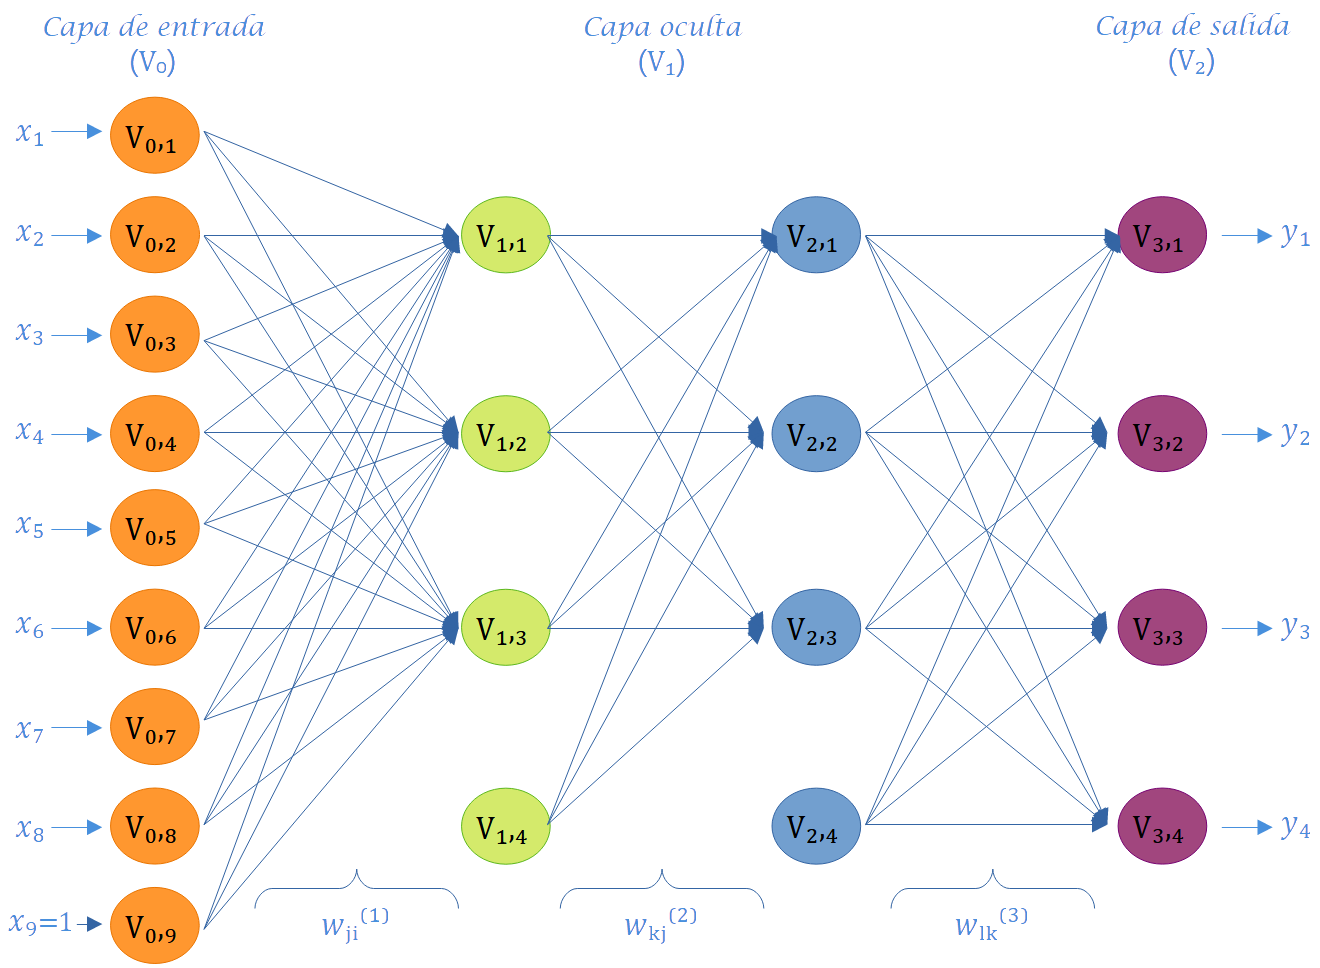
\includegraphics{Imagenes/RNP.png}

}

\caption{\label{fig-rnp}Red neuronal artificial profunda feedforward con
ocho variables de entrada, cuatro variables de salida y dos capas
ocultas con tres neuronas cada una.}

\end{figure}%

A continuación, se definen los tipos de neuronas:

\begin{enumerate}
\def\labelenumi{\arabic{enumi}.}
\item
  \textbf{Neurona de entrada}: Una neurona que recibe entradas externas
  desde fuera de la red.
\item
  \textbf{Neurona de salida}: Una neurona que produce algunas de las
  salidas de la red.
\item
  \textbf{Neurona oculta}: Una neurona que no tiene interacción directa
  con el ``mundo exterior'' sino solo con otras neuronas dentro de la
  red. Una terminología similar se utiliza a nivel de capa para redes
  neuronales multicapa.
\end{enumerate}

Como se aprecia en la Figura~\ref{fig-rnp}, la disposición de las
neuronas en una red neuronal artificial se lleva a cabo mediante la
formación de niveles que contienen un número específico de neuronas.
Cuando un conjunto de neuronas artificiales recibe simultáneamente el
mismo tipo de información, se le denomina capa. Además, se hace
referencia a una red compuesta por tres tipos de niveles como capas. La
Figura~\ref{fig-estructuras} exhibe otras seis redes con diversos
números de capas, y la mitad de ellas (Figura~\ref{fig-a},
Figura~\ref{fig-c}, Figura~\ref{fig-e}) son univariadas, ya que la
variable de respuesta a predecir es única, mientras que la otra mitad
(Figura~\ref{fig-b}, Figura~\ref{fig-d}, Figura~\ref{fig-f}) son
multivariadas, dado que la red tiene el propósito de predecir dos
salidas. Es relevante destacar que los paneles a y b en la
Figura~\ref{fig-estructuras} representan redes con solo una capa y sin
capas ocultas; por consiguiente, este tipo de redes corresponde a
modelos convencionales de regresión o clasificación por regresión.

\begin{figure}

\begin{minipage}{0.50\linewidth}

\centering{

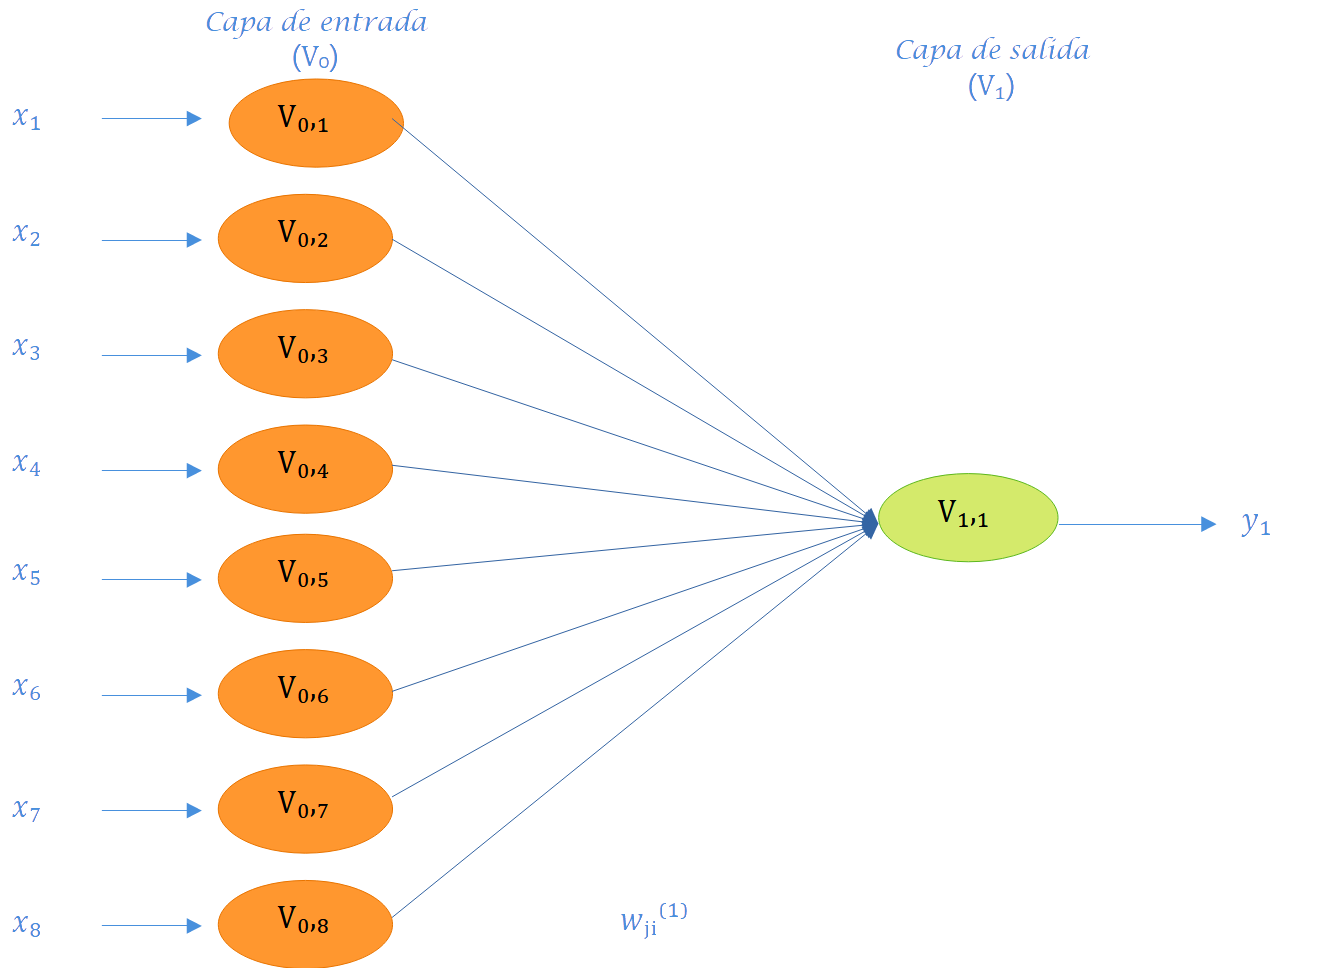
\includegraphics{Imagenes/a.png}

}

\subcaption{\label{fig-a}Salida unicapa y univariante.}

\end{minipage}%
%
\begin{minipage}{0.50\linewidth}

\centering{

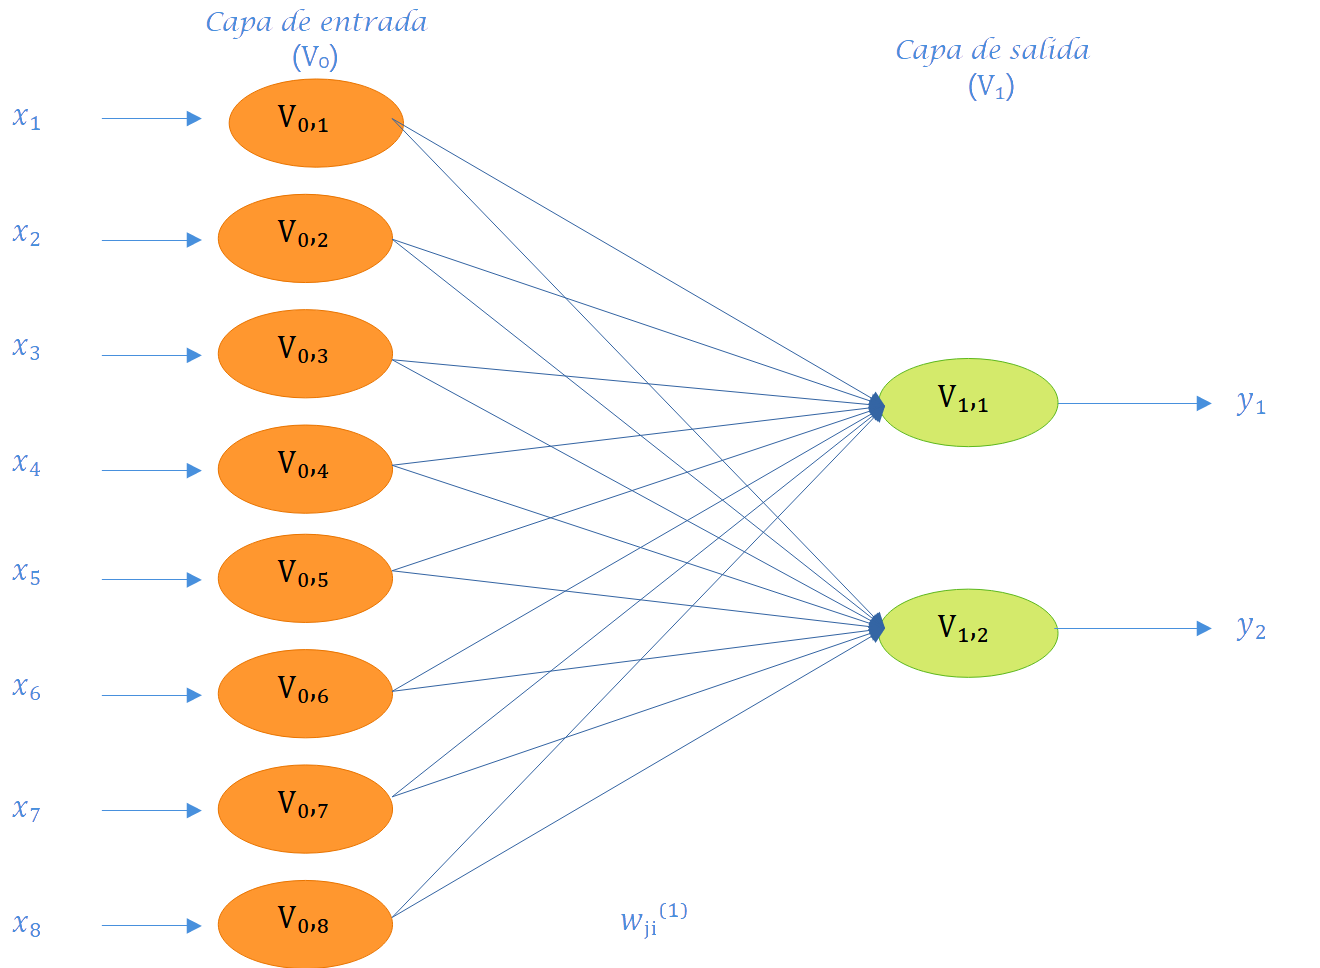
\includegraphics{Imagenes/b.png}

}

\subcaption{\label{fig-b}Salida unicapa y multivariante.}

\end{minipage}%
\newline
\begin{minipage}{0.50\linewidth}

\centering{

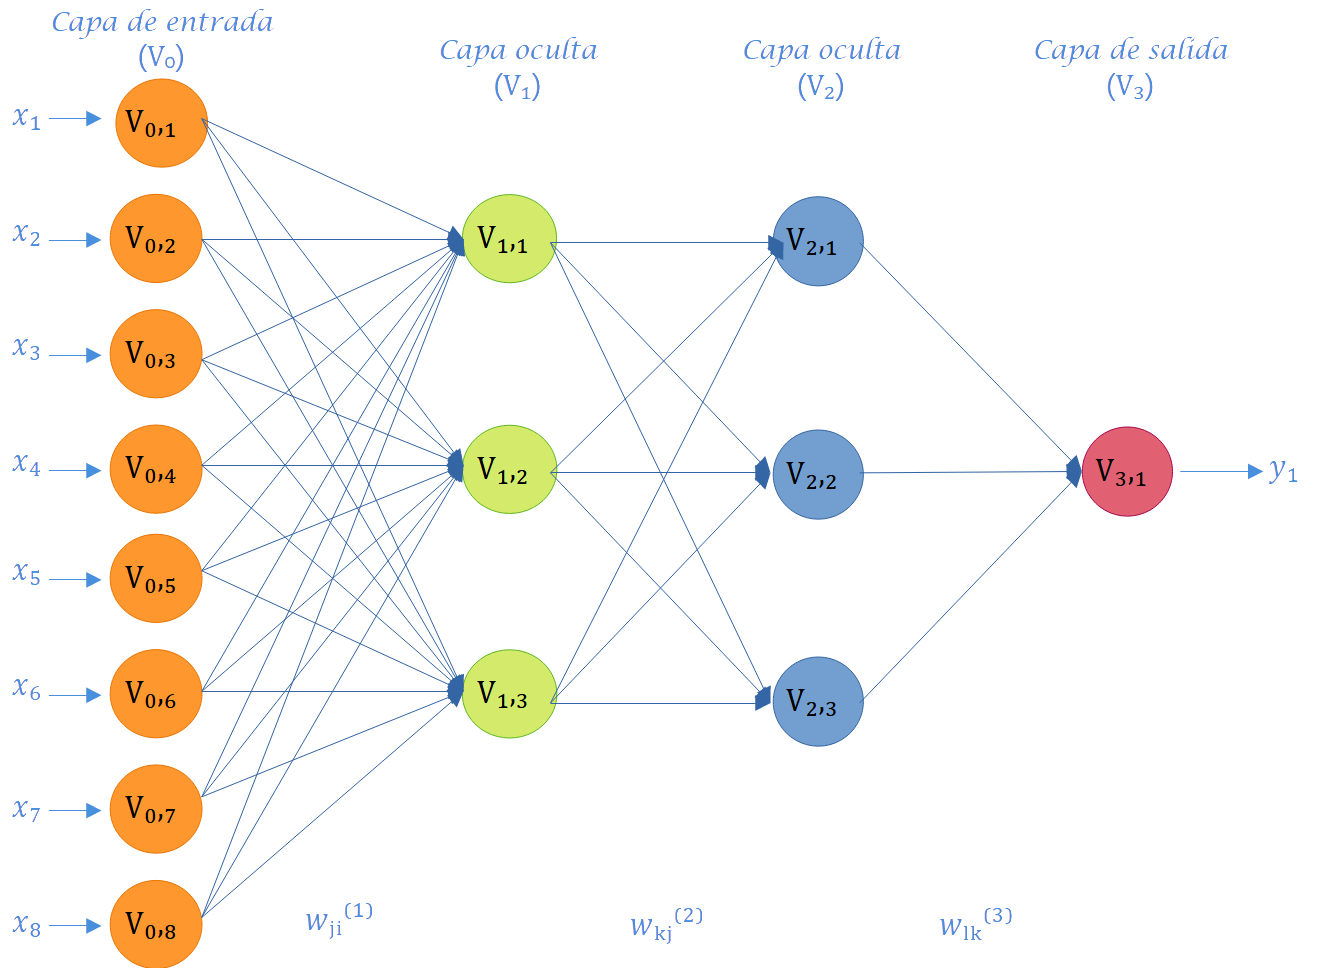
\includegraphics{Imagenes/c.png}

}

\subcaption{\label{fig-c}Salida univariante y de tres capas.}

\end{minipage}%
%
\begin{minipage}{0.50\linewidth}

\centering{

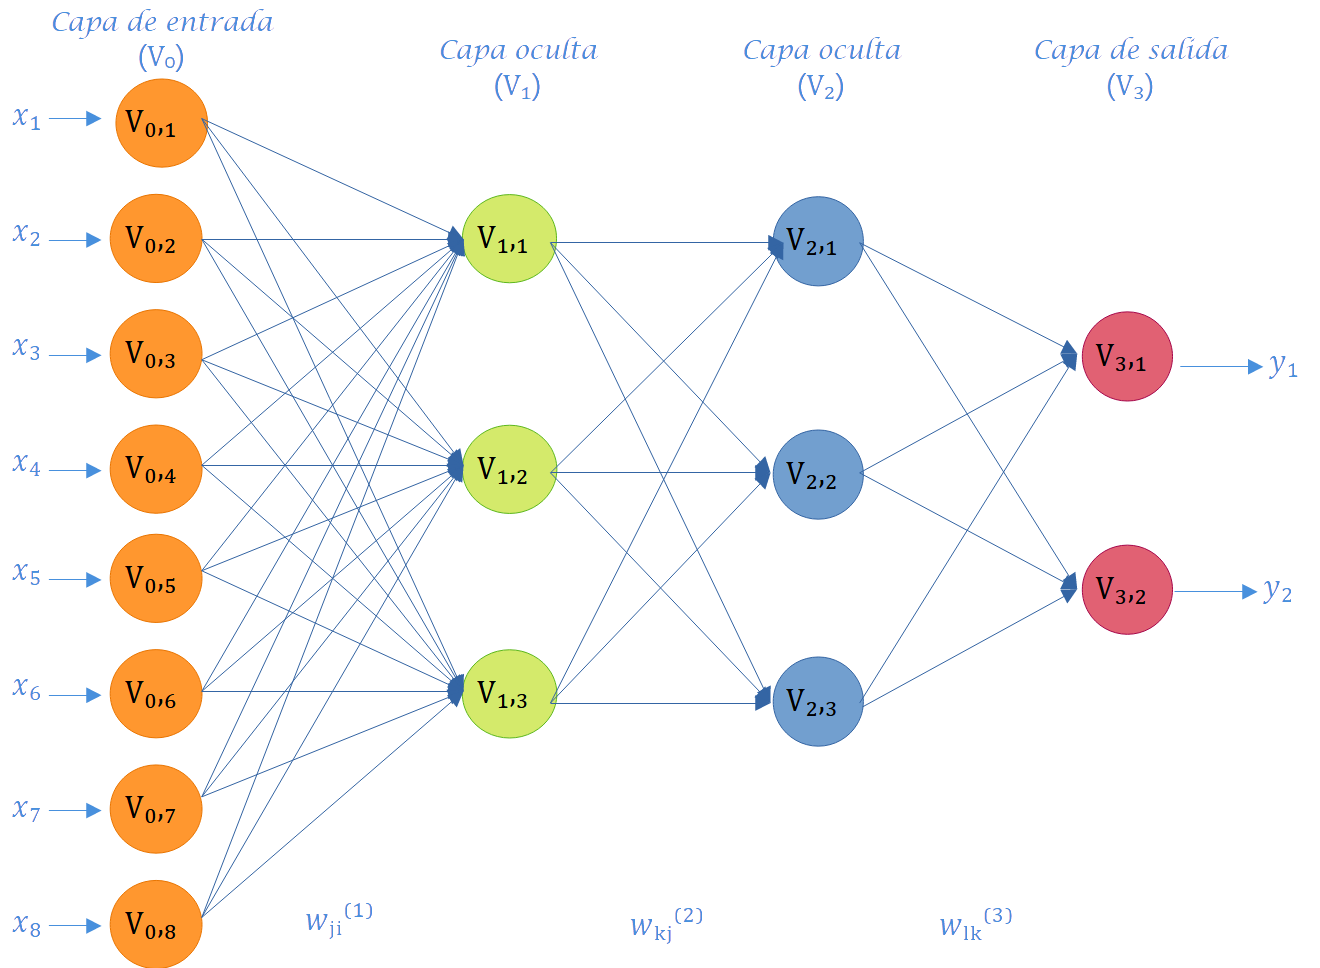
\includegraphics{Imagenes/d.png}

}

\subcaption{\label{fig-d}Salida multivariante y de tres capas.}

\end{minipage}%
\newline
\begin{minipage}{0.50\linewidth}

\centering{

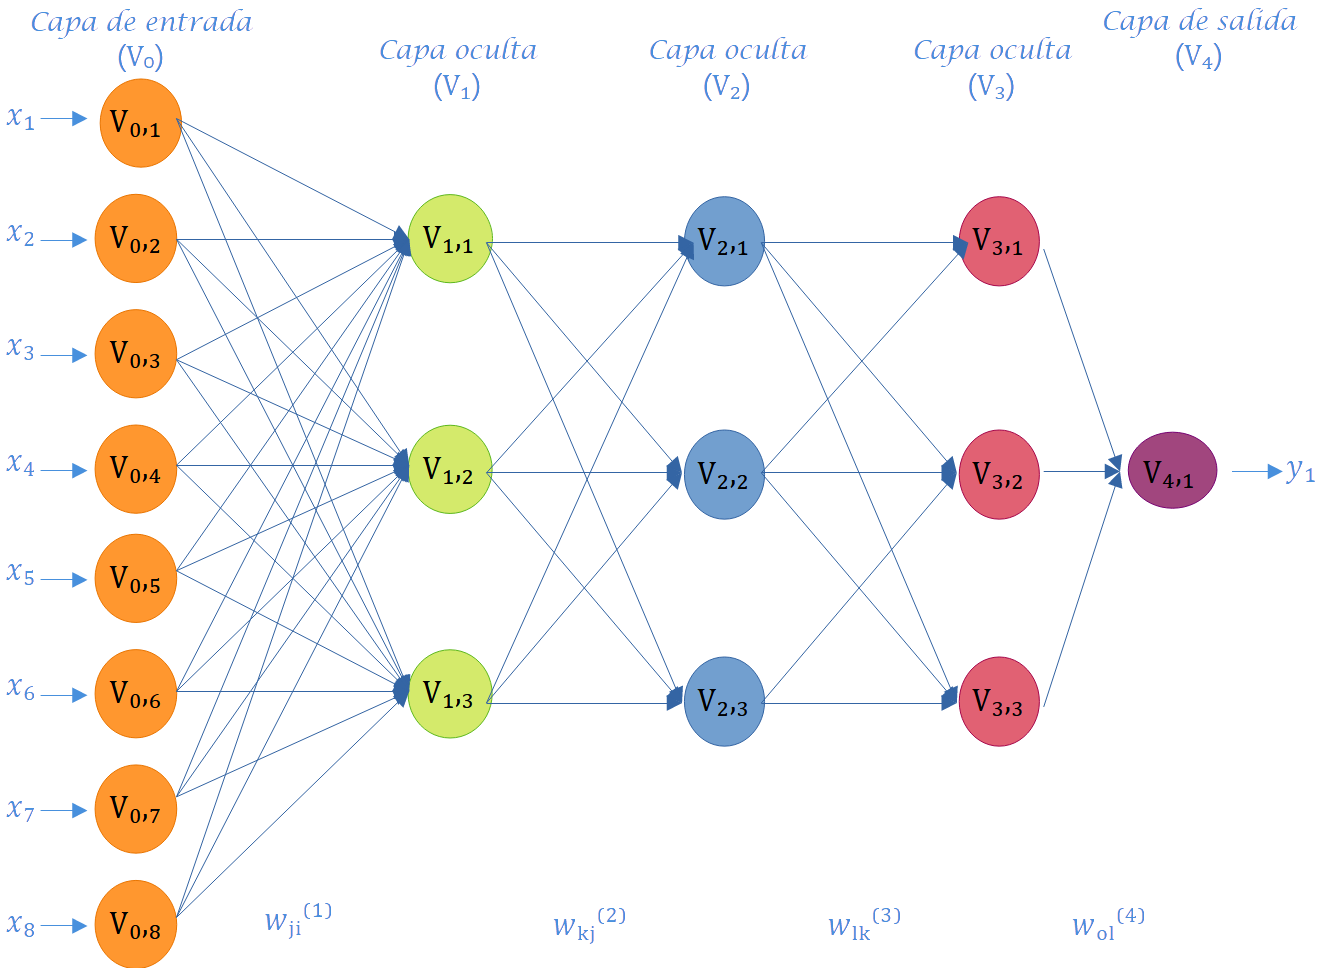
\includegraphics{Imagenes/e.png}

}

\subcaption{\label{fig-e}Salida univariante de cuatro capas.}

\end{minipage}%
%
\begin{minipage}{0.50\linewidth}

\centering{

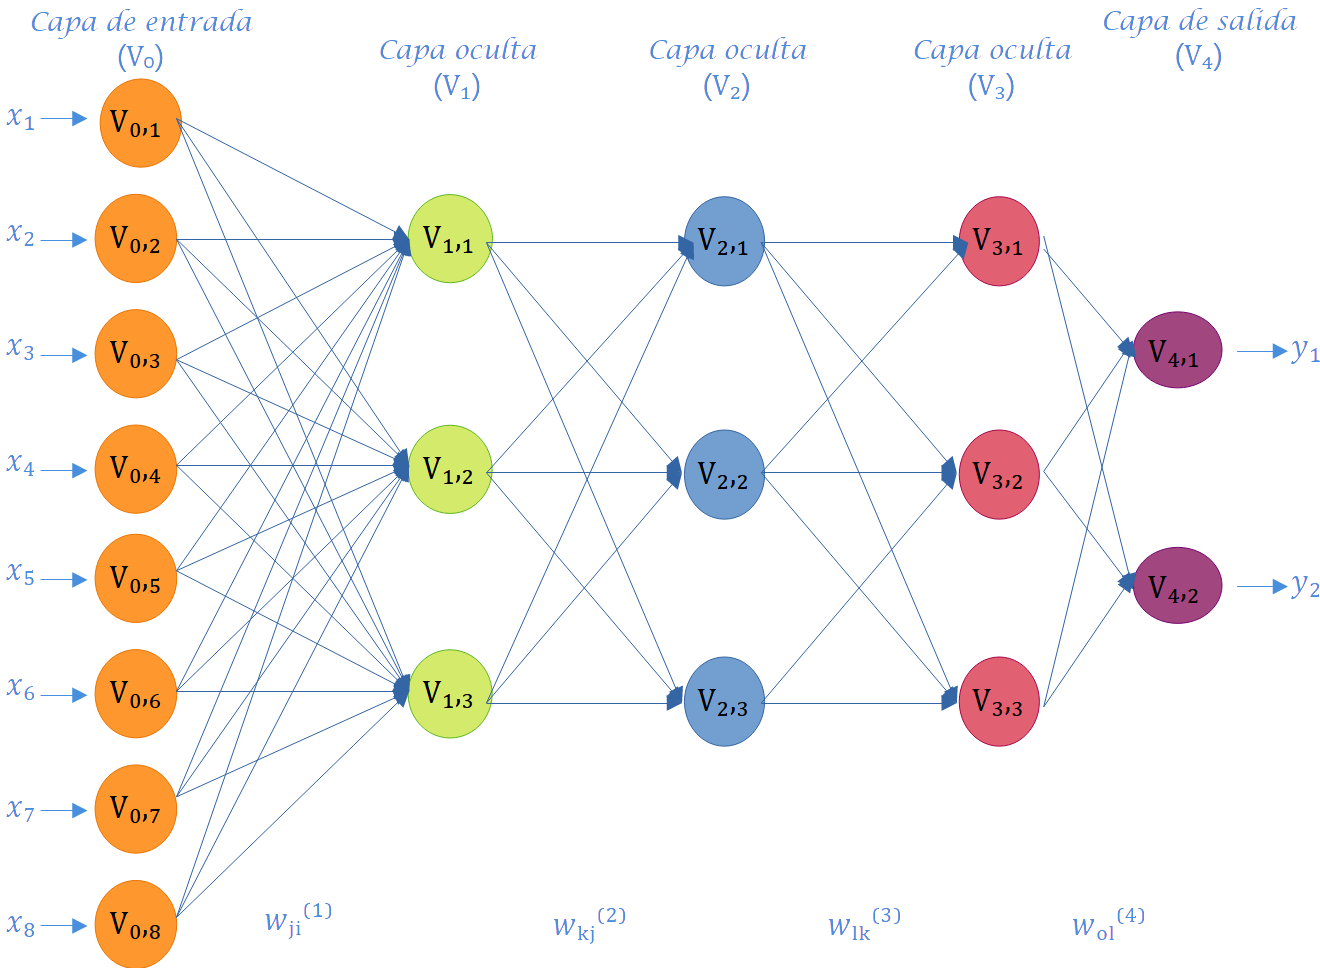
\includegraphics{Imagenes/f.png}

}

\subcaption{\label{fig-f}Salida multivariante de cuatro capas.}

\end{minipage}%

\caption{\label{fig-estructuras}Diferentes estructuras de redes
neuronales univariadas y multivariadas.}

\end{figure}%

En consecuencia, la arquitectura de una red neuronal artificial se
refiere a la manera en que las neuronas están organizadas en la red, y
está estrechamente vinculada al algoritmo de aprendizaje empleado para
entrenar la red. Según el número de capas, clasificamos las redes como
monocapa o multicapa; y si consideramos la dirección del flujo de
información como criterio clasificatorio, las redes se denominan de
avance o recurrentes. Cada tipo de arquitectura se aborda la siguiente
sección.

\section{Arquitectura}\label{arquitectura}

\subsection{Perceptrón simple}\label{perceptruxf3n-simple}

El \emph{perceptrón simple} consta de cuatro componentes fundamentales
en su estructura. Estos son: las entradas (input) con conexiones y pesos
(nodos ponderados), el nodo de procesamiento o suma, la función de
activación y las salidas (output). El nodo de procesamiento realiza una
regresión lineal, involucrando la suma ponderada de los pesos en cada
nodo de las entradas y un término de sesgo o término independiente. En
esencia, el perceptrón simple funciona como un discriminador lineal que,
a partir de un umbral establecido, produce una salida binaria.

Desde una perspectiva matemática, el perceptrón simple se representa
mediante la siguiente ecuación:

\begin{equation}\phantomsection\label{eq-perceptron}{
\hat{\mathbf{y}}(\mathbf x)=f(\mathbf w^T\mathbf x+b).
}\end{equation}

La arquitectura que modela esta ecuación se describe a través de la
Figura~\ref{fig-arqper},

\begin{figure}

\centering{

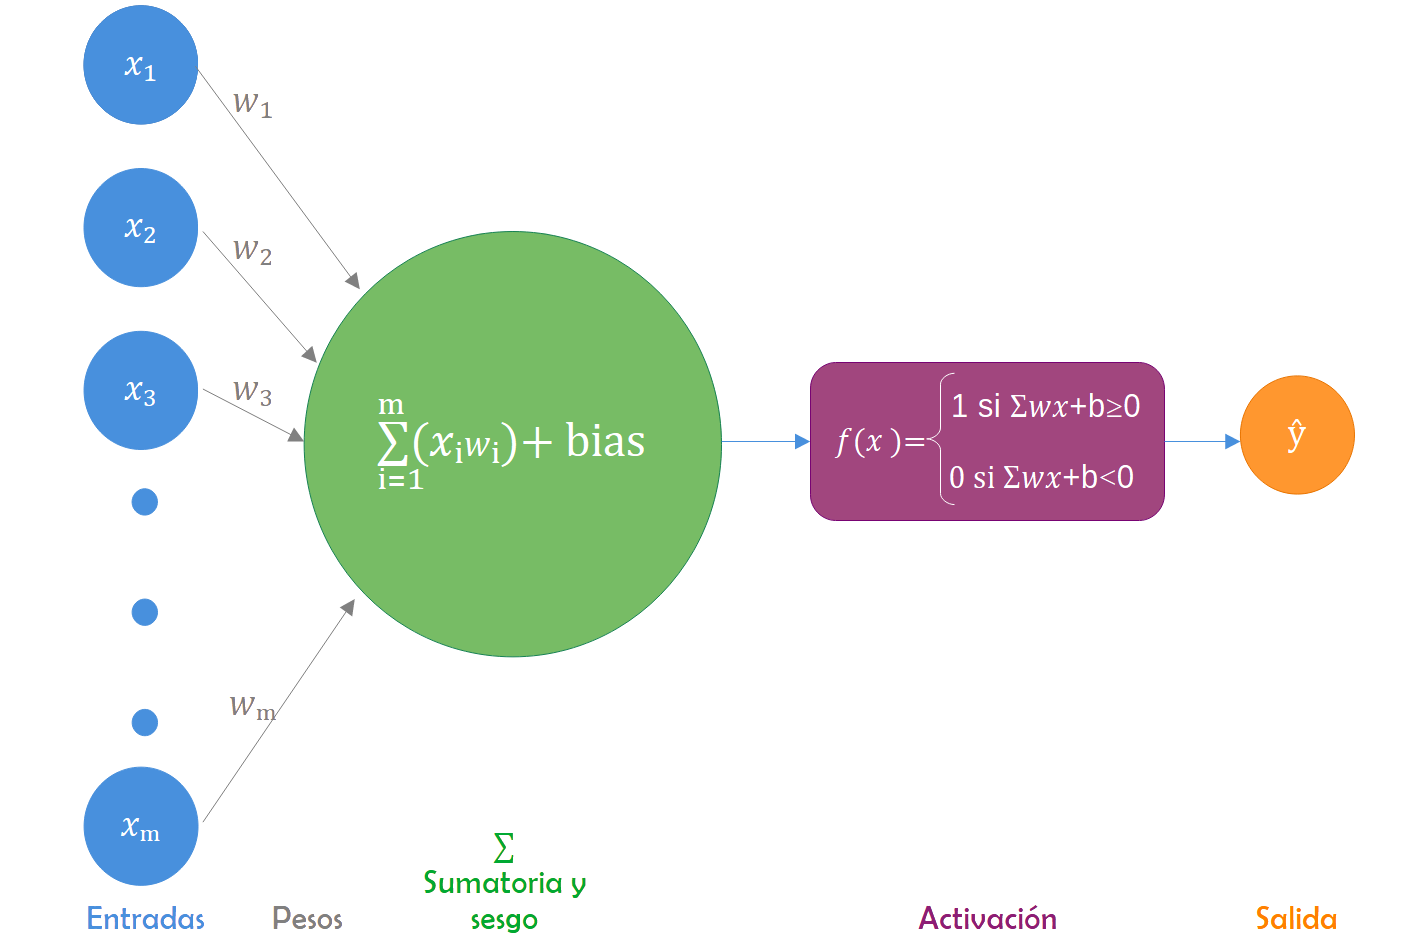
\includegraphics{Imagenes/perceptron.png}

}

\caption{\label{fig-arqper}Arquitectura de un perceptrón simple}

\end{figure}%

donde \(\mathbf x\) denota el vector de entradas, \(\mathbf w\) denota
el vector de pesos asociados a cada nodo, \(b\) denota el sesgo o
intercepto de la regresión, \(\sum\) denota el nodo de procesamiento o
combinador lineal y \(f\) denota la función de activación o función
limitadora, siendo esta última una transformación no lineal de la
regresión obtenida en el nodo de procesamiento.

Aunque el perceptrón simple demuestra eficacia en el aprendizaje y la
resolución de problemas linealmente separables, como las compuertas
lógicas \emph{AND} (Figura~\ref{fig-and}) y \emph{OR}
(Figura~\ref{fig-or}) , presenta limitaciones en la resolución de
problemas que no son de este tipo. Un ejemplo paradigmático de ello es
su incapacidad para clasificar las salidas de una compuerta lógica del
tipo \emph{XOR} (Figura~\ref{fig-xor}), ya que el nodo de procesamiento
solo permite la separación de la información mediante una única recta de
regresión.

\begin{figure}

\begin{minipage}{0.33\linewidth}

\centering{

\captionsetup{labelsep=none}

\begin{figure}[H]

{\centering 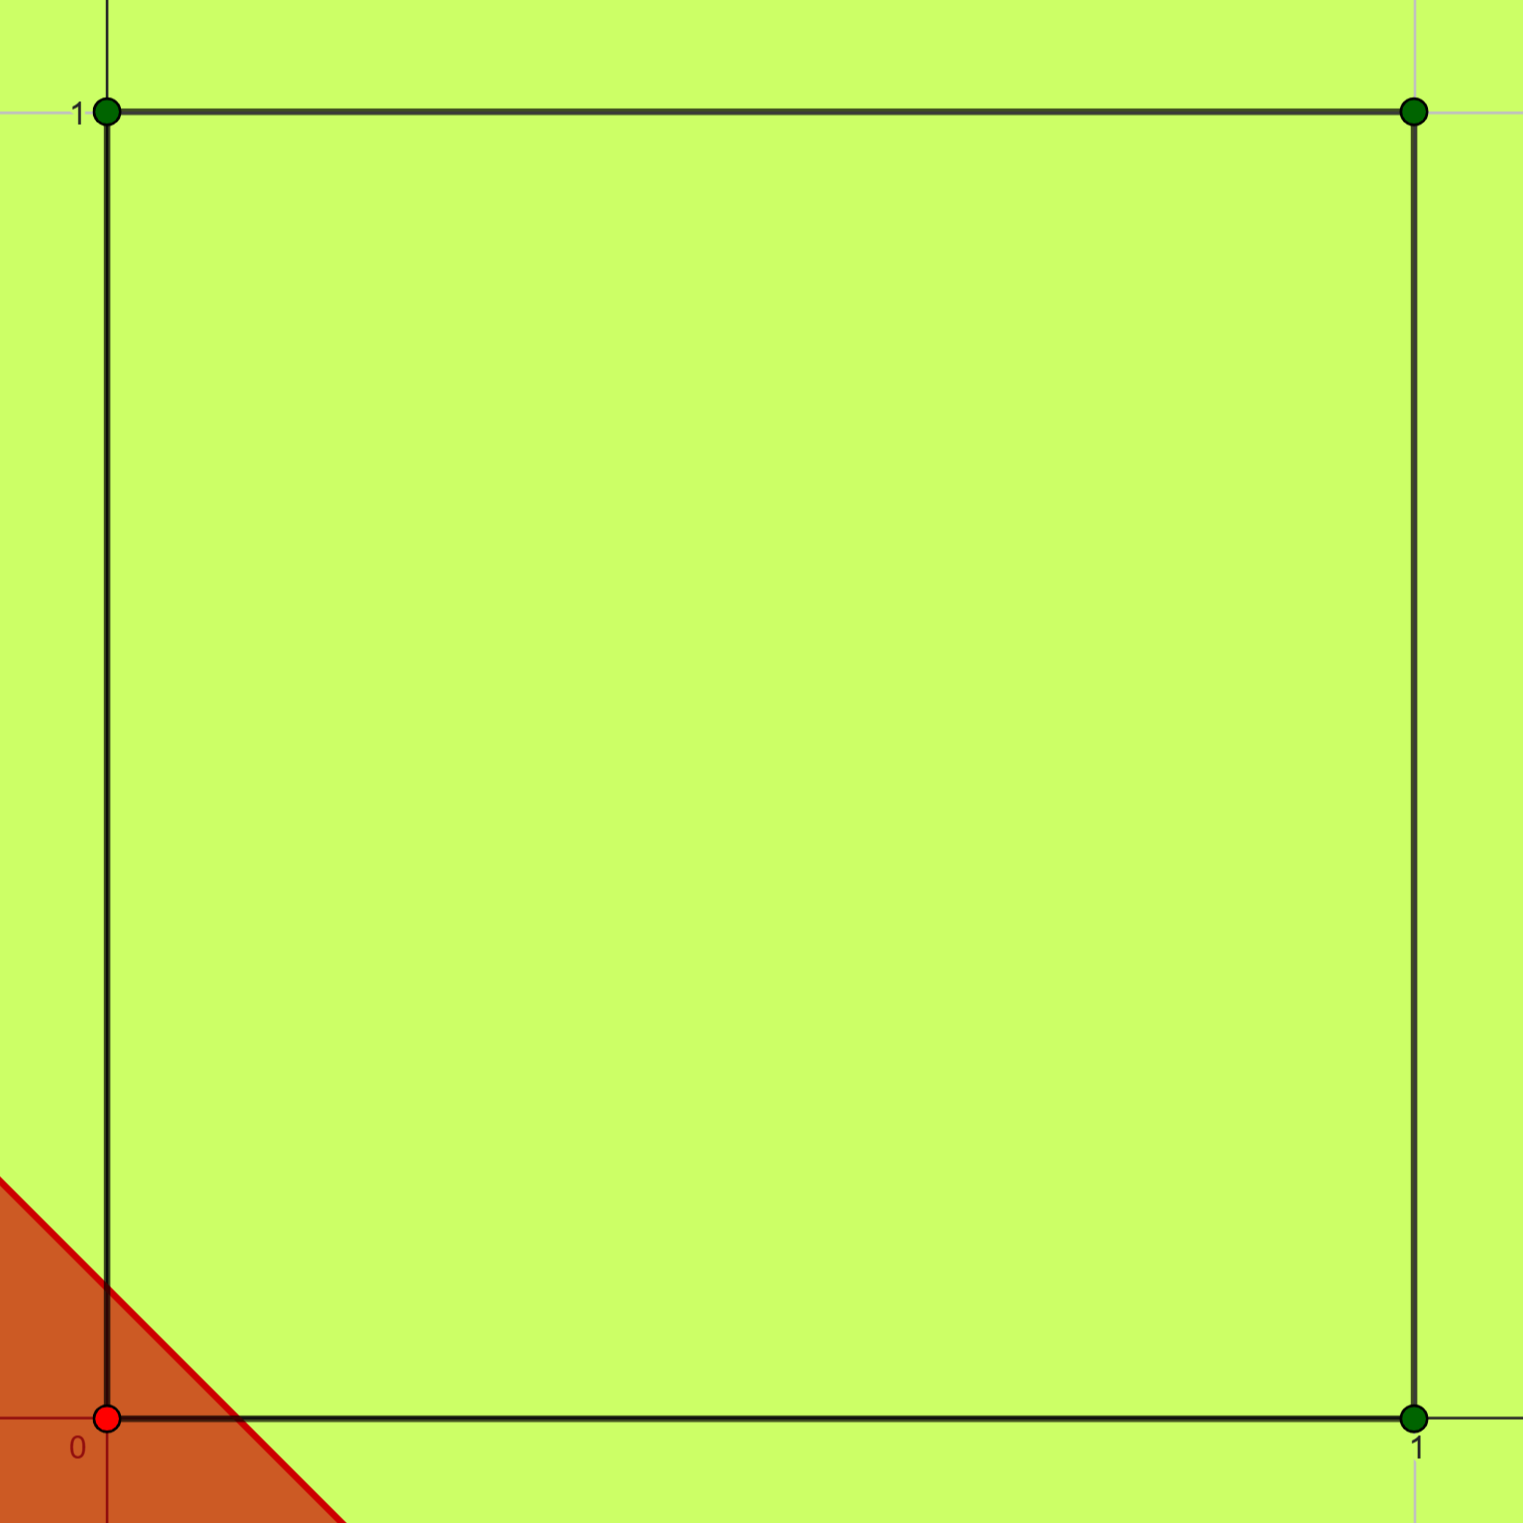
\includegraphics{Imagenes/or.png}

}

\subcaption{OR}

\end{figure}%

}

\subcaption{\label{fig-or}}

\end{minipage}%
%
\begin{minipage}{0.33\linewidth}

\centering{

\captionsetup{labelsep=none}

\begin{figure}[H]

{\centering 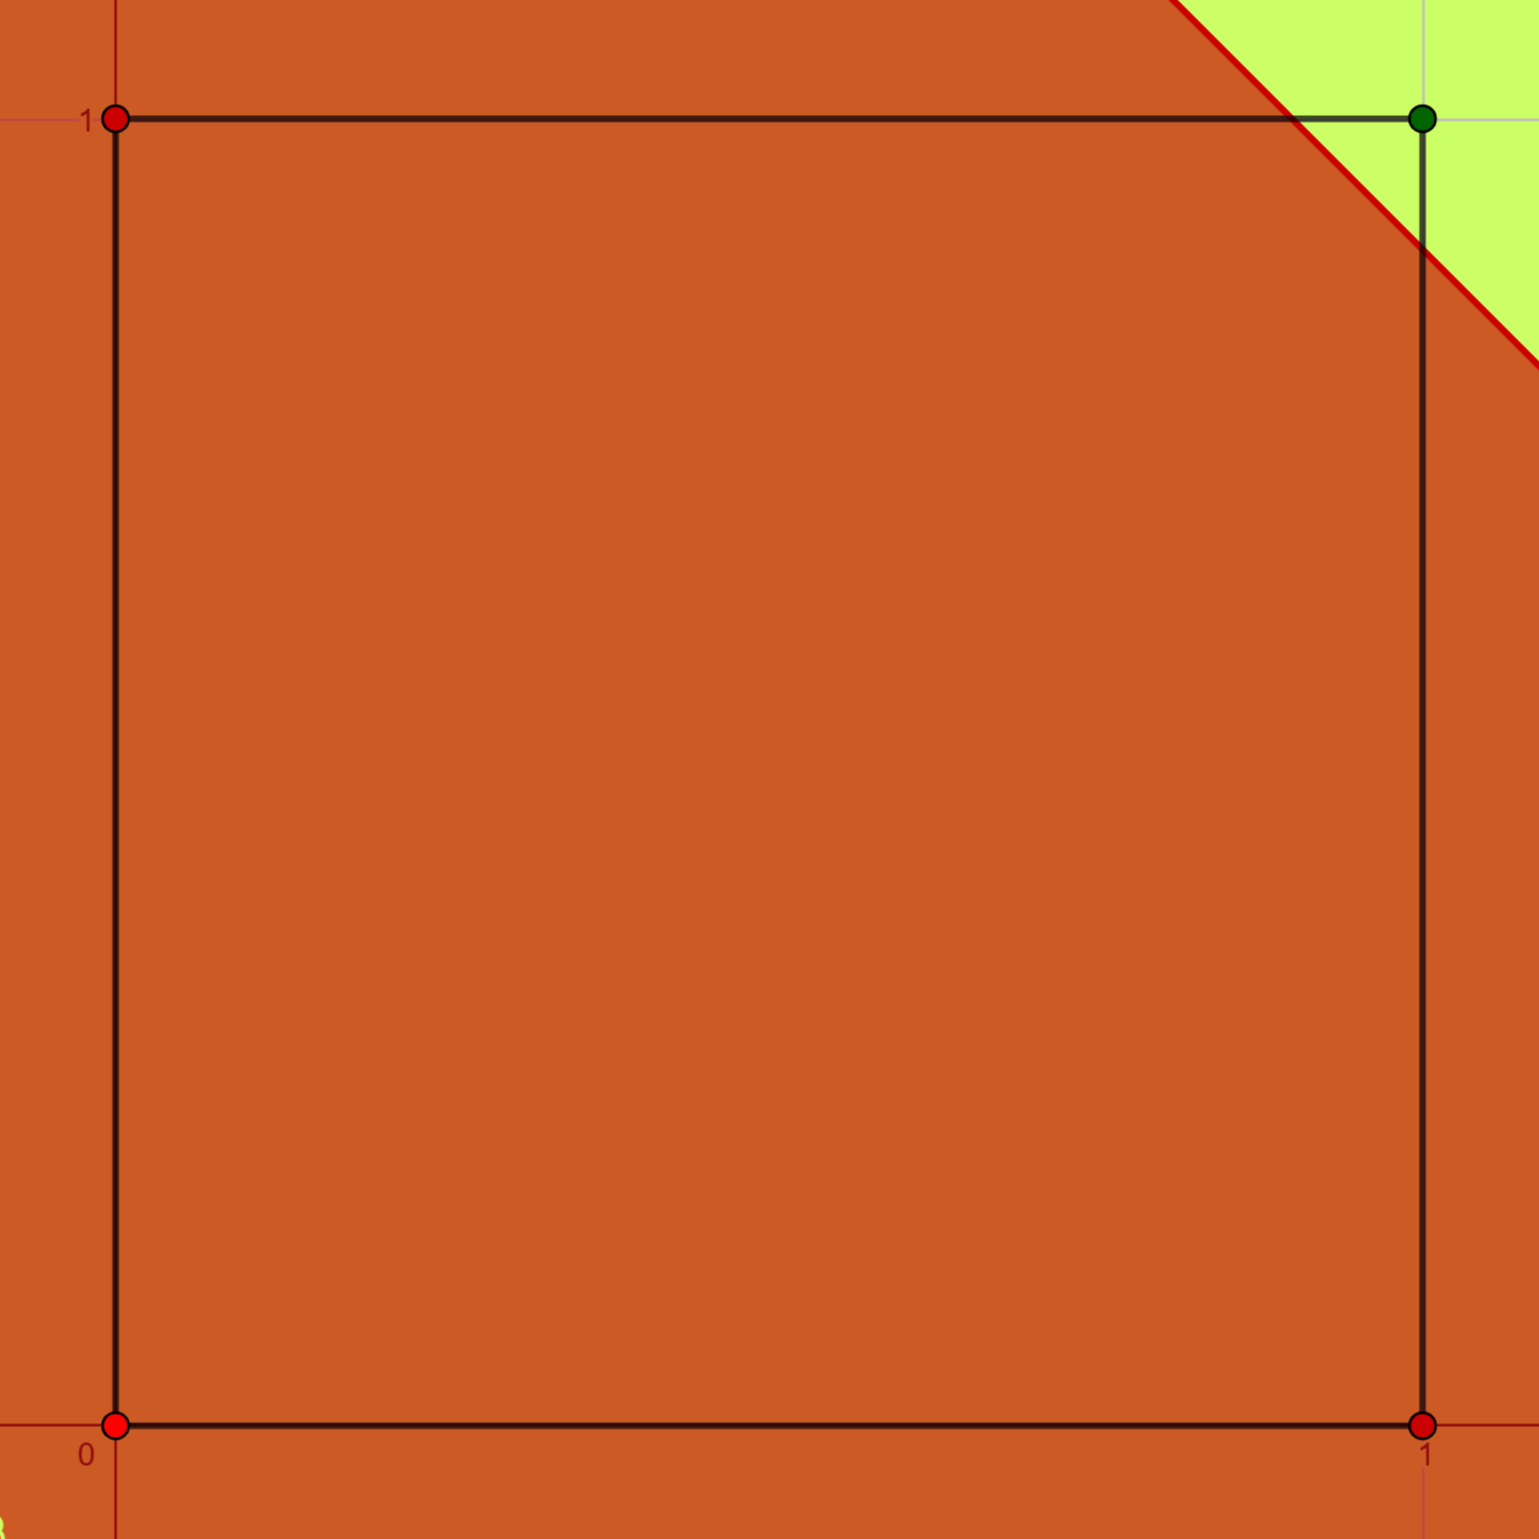
\includegraphics{Imagenes/and.png}

}

\subcaption{AND}

\end{figure}%

}

\subcaption{\label{fig-and}}

\end{minipage}%
%
\begin{minipage}{0.33\linewidth}

\centering{

\captionsetup{labelsep=none}

\begin{figure}[H]

{\centering \includegraphics{Imagenes/XOR.png}

}

\subcaption{XOR}

\end{figure}%

}

\subcaption{\label{fig-xor}}

\end{minipage}%

\caption{\label{fig-compuertas}Compuertas lógicas.}

\end{figure}%

\subsection{Perceptrón Multicapa (MLP)}\label{sec-arqmlp}

La solución al problema de la puerta lógica \emph{XOR} consiste en la
adición de una neurona adicional, permitiendo así la definición de una
nueva recta de regresión, como se ilustra en la Figura~\ref{fig-xor}.
Esto conduce a la creación de lo que se conoce como \emph{Perceptrón
Multicapa} o \emph{MLP} (por sus siglas en inglés), también reconocido
como \emph{Red Neuronal Profunda}. Esta estructura representa una
generalización del perceptrón simple, incorporando más de un nivel de
neuronas y/o una o varias capas de neuronas ``entre'' la capa de
entradas y la capa de salidas, las cuales son denominadas capas ocultas.
En estas capas ocultas, las funciones de activación entre las neuronas
no son necesariamente lineales. Las MLP son consideradas las redes
neuronales artificiales por defecto y se representan mediante un
diagrama simple, que transmite las entradas de capa en capa hasta
alcanzar la capa final.

La red neuronal de la Figura~\ref{fig-mlp} ejemplifica un MLP de dos
capas ocultas. En esta representación, los superíndices indican la
posición en las capas, mientras que los subíndices indican la posición
relativa de cada nodo en su respectiva capa. La red consta de un vector
de entradas \(\mathbf{x} \in \mathbb{R}^{d_0}\), donde
\(\mathbf{x} = (x_1, \ldots, x_{d_0})^T\), capas ocultas denotadas por
\(a^l\), y un vector de salidas \(\hat{y} \in \mathbb{R}^{d_L}\) con
\(\hat{y} = (\hat{y}_1, \ldots,\hat y_{d_L})^T\). Las capas ocultas
contienen nodos de procesamiento o neuronas representadas por
\(a = f(z)\), donde \(f\) es la función de activación de cada capa y
\(z\) es un combinador lineal (matricial). Las conexiones entre las
capas están ponderadas por \(\mathbf{w}\), que representa las matrices
de pesos asociadas en cada capa. Por ejemplo, \(w_{ij}^1\) representa el
peso asociado a la conexión entre la entrada j-ésima y el i-ésimo nodo
de procesamiento en la primera capa oculta. Las matrices
\(\mathbf{w}^l\) tienen dimensiones \((d_l \times d_{l-1})\), donde la
capa de entrada se considera como capa cero \((l = 0)\).

Es importante destacar que el término \(b\), que indica el sesgo en el
perceptrón simple, también se incluye en la red MLP en cada nodo de
procesamiento, específicamente en el combinador lineal \(z\). A partir
de este momento, el nodo de procesamiento incorporará el término de
sesgo \(b\), y \(b^1 \in a^1\) denotará el vector de sesgo en la primera
capa oculta.

\begin{figure}

\centering{

\includegraphics{Imagenes/mlp.png}

}

\caption{\label{fig-mlp}Red neuronal MLP con dos capas ocultas (Sosa
Jerez, Zamora Alvarado, et~al. (s.~f.)).}

\end{figure}%

La ecuación matemática que describe la red de la Figura~\ref{fig-mlp} es
la siguiente:

\[
\begin{split}\hat{\mathbf{y}} &= f^3(z^3) \\&= f^3(\mathbf{w}^3 a^2 + b^3) \\&= f^3(\mathbf{w}^3 (f^2(z^2)) + b^3) \\&= f^3(\mathbf{w}^3 (f^2(\mathbf{w}^2 a^1 + b^2)) + b^3) \\&= f^3(\mathbf{w}^3 (f^2(\mathbf{w}^2 (f^1(z^1)) + b^2)) + b^3) \\&= f^3(\mathbf{w}^3 (f^2(\mathbf{w}^2 (f^1(\mathbf{w}^1 \mathbf{x} + b^1)) + b^2)) + b^3).\end{split}
\]

Se observa que \(f^3\) representa la función de activación en la capa de
salida, la cual comúnmente se elige como la identidad. Sin embargo, en
algunos modelos de clasificación, la predicción puede ser más precisa si
esta función es no lineal y limitadora.

Por otro lado, la última columna en la Figura~\ref{fig-mlp} constituye
una capa adicional en la cual, a través de una función de pérdida, se
evalúa el rendimiento de la red. Esta evaluación relaciona la
información obtenida en la capa de salida con los datos esperados en un
modelo de aprendizaje supervisado.

\section{Perceptrón}\label{perceptruxf3n}

En un principio, se establece un conjunto de datos a estudiar denominado
\(\mathbf X \subseteq \mathbb R^{m+1}\). Este conjunto se particiona en
dos clases linealmente separables, \(\mathscr C_1\) y \(\mathscr C_2\).
A los vectores \(\mathbf x = (x_1, x_2,...,x_m,1)^T\) que pertenecen a
\(\mathbf X\), se les denomina \emph{entradas}.

A continuación, se introduce un conjunto
\(\mathbf W \subseteq \mathbb R^{m+1}\), que contiene etiquetas para los
nodos del perceptrón. Los elementos de este conjunto, denotados como
\(\mathbf w = (w_1,w_2,...,w_m,b)^T\), se llaman \emph{pesos
sinápticos}. Aquí, \(b\) es un número real fijo conocido como
\emph{sesgo}. Con el propósito de describir el algoritmo del Perceptrón,
se presentan cuatro definiciones fundamentales:

\begin{definition}[Clases linealmente
separables]\protect\hypertarget{def-cls}{}\label{def-cls}

Sean \(\mathscr C_1\) y \(\mathscr C_2\) dos clases en un espacio
\(n-\)dimensional. \(\mathscr C_1\) y \(\mathscr C_2\) se consideran
clases linealmente separables si existe un vector
\(\mathbf w \in \mathbb R^{m+1}\) de pesos sinápticos que cumple con las
siguientes condiciones: \[
\begin{split}
\mathbf w^T \mathbf x_1 &> 0\text{ para cada vector de entrada } \mathbf x_1 \in \mathscr C_1.\\
\mathbf w^T \mathbf x_2 &\leq 0\text{ para cada vector de entrada } \mathbf x_2 \in \mathscr C_2.
\end{split}
\]

\end{definition}

\begin{definition}[Combinador
lineal]\protect\hypertarget{def-comlin}{}\label{def-comlin}

Dados \(\mathbf x = (x_1, x_2,..., x_m,1)^T\) y
\(\mathbf w = (w_1,w_2,...,w_m,b)^T\), se define la función
\(\mathcal V: \mathbb R^{m+1}\times\mathbb R^{m+1} \rightarrow \mathbb R\)
como \(\mathcal V(\mathbf x, \mathbf w) = \mathbf w^T\mathbf x\), donde
\(\mathcal V(\mathbf x, \mathbf w) = 0\) representa el hiperplano de
separación entre dos regiones de decisión.

\end{definition}

\begin{definition}[Función
limitadora]\protect\hypertarget{def-flim}{}\label{def-flim}

Sea \(\mathscr A\) el conjunto de todas las combinaciones lineales
\(\mathcal V(\mathbf x, \mathbf w)\). Considerando \(t \in \mathscr A\),
se define la función limitadora \(g\) como sigue: \[
\begin{split}
g: \mathscr A &\rightarrow \{1,-1\}\\
t &\rightarrow g(t)= \begin{cases} 1 & \text{si }\quad t> 0,\\ \\-1 & \text{si }\quad t\leq 0.\end{cases}
\end{split}
\]

\end{definition}

\begin{definition}[Función
perceptrón]\protect\hypertarget{def-fper}{}\label{def-fper}

Dadas \(\mathcal V(\mathbf x, \mathbf w)\) y \(g(t)\), se define la
aplicación clasificadora
\(\mathscr P: \mathbb R^{m+1}\times \mathbb R^{m+1} \rightarrow \{1,-1\}\)
como
\(\mathscr P(\mathbf x, \mathbf w)=g(\mathcal V(\mathbf x, \mathbf w))=\hat{y}\),
donde \(\hat{y}\in \{-1,1\}\) es la salida de la función perceptrón.
Además, la aplicación perceptrón posee una representación gráfica
mediante un dígrafo simple, como se muestra en la
Figura~\ref{fig-arqper}.

\end{definition}

A través de la función establecida en la Definición~\ref{def-fper}, se
desarrolla un modelo de aprendizaje supervisado de clasificación binaria
denominado \emph{Perceptrón}. Este modelo involucra las funciones
previamente definidas con el objetivo de clasificar correctamente un
conjunto de entradas \(\mathbf X\), linealmente separables en dos
clases. Se aplica una regla de aprendizaje adaptativa sobre cada uno de
los pesos sinápticos \((\mathbf w)\) en una cantidad finita de pasos
\((n)\), proceso conocido como \emph{algoritmo de aprendizaje del
Perceptrón}.

\begin{definition}[Combinador lineal del
perceptrón]\protect\hypertarget{def-clp}{}\label{def-clp}

Considerando las entradas y los pesos sinápticos en el perceptrón,
\(\mathbf x(n) = (x_1(n), x_2(n),...,x_m(n),1)^T\) y
\(\mathbf w(n) = (w_1(n),w_2(n),...,w_m(n),b)^T\), se define el
combinador lineal del perceptrón como

\[
\mathcal V=\mathbf w^T(n)\mathbf x(n),
\]

donde \(n\) denota el número de iteraciones en la aplicación del
algoritmo.

\end{definition}

Se considera \(\mathscr H \subset \mathbf X\) como el subsepacio
vectorial de entrenamiento. \(\mathscr H_1\) es el subespacio de
vectores de entrenamiento \(\mathbf x_1(1),\mathbf x_1(2),...\) que
pertenecen a la clase \(\mathscr C_1\), y \(\mathscr H_2\) es el espacio
de vectores de entrenamiento \(\mathbf x_2(1),\mathbf x_2(2),...\) que
pertenecen a la clase \(\mathscr C_2\). Se define
\(\mathscr H= \mathscr H_1\cup \mathscr H_2\). Con el fin de evitar un
sobreentrenamiento en alguna de las dos clases, se garantiza que
\(\mathscr H_1\) y \(\mathscr H_2\) tengan la misma cardinalidad.

Dado que el perceptrón es un modelo de aprendizaje supervisado, se
establece \(y(k) \in \{-1,1\}\) como la clase a la que realmente
pertenece cada entrada \(x(k)\) de \(\mathscr H\). Se observa que el
valor \(y(k) - \hat{y}(k)\) representa el error cometido por el
Perceptrón en su clasificación, y de este error se deriva la siguiente
definición:

\begin{definition}[Función actualización por corrección del
error]\protect\hypertarget{def-face}{}\label{def-face}

Se define la regla de actualización de los pesos sinápticos como sigue:

\[
\mathbf w(n+1)=\mathbf w(n)+\eta(n)[y(n)-\hat y(n)]x(n).
\]

De esta manera,

\[
 \mathbf{w}(n+1) = \left\{\begin{array}{lcc} \mathbf w(n)+2\eta(n) x(n)& si & y(n)=1 \text{ y }\hat{y}=-1,\\ \\\mathbf w(n) & si & y(n)=\hat{y}(n),\\ \\ \mathbf w(n)-2\eta(n)x(n) & si & y(n)=-1 \text{ y }\hat{y}=1, \end{array}\right.
\]

donde \(\eta(n)=\eta>0\) es una regla de adaptación de incremento fijo
llamada \emph{tasa de aprendizaje}.

\end{definition}

\subsection{Teorema de convergencia del
perceptrón}\label{teorema-de-convergencia-del-perceptruxf3n}

\begin{theorem}[]\protect\hypertarget{thm-tcp}{}\label{thm-tcp}

Sean \(\mathscr H_1\) y \(\mathscr H_2\), subconjuntos de vectores de
entrenamiento linealmente separables. Considere las \(m\) entradas
presentadas al perceptrón, como elementos de estos dos subconjuntos. El
perceptrón converge después de \(n_0\) iteraciones, en el sentido que:

\[
\mathit w(n_0)=\mathit w(n_0+1)=\mathit w(n_0+2)=\cdots,
\] es un vector solución para \(n_0\leq n_{\max}\).

\begin{proof}
Vea Sosa Jerez, Zamora Alvarado, et~al. (s.~f.).
\end{proof}

\end{theorem}

\section{Funciones de activación}\label{funciones-de-activaciuxf3n}

La asignación entre las entradas y una capa oculta en una Red Neuronal
Artificial (RNA) y una Red Neuronal Profunda (RNP) es determinada por
funciones de activación. Dichas funciones propagan la información
generada mediante la combinación lineal de los pesos y las entradas
hacia la siguiente capa, incluyendo la capa de salida. Como se ha
mencionado anteriormente, existe una analogía entre las neuronas
biológicas y las redes neuronales artificiales; en este contexto, las
funciones de activación son análogas a la tasa del potencial de acción
disparado en el cerebro.

Las funciones de activación son transformaciones de funciones escalares
a escalares que proporcionan una salida específica para cada neurona.
Estas funciones introducen no linealidades en las capacidades de
modelado de la red. La función de activación de una neurona (nodo)
define la forma funcional de su activación. Por ejemplo, si se define
una función de activación lineal como \(g(z) = z\), el valor de la
neurona sería la entrada cruda \(x\) multiplicada por el peso aprendido,
representando así un modelo lineal. A continuación, se describen las
funciones de activación más populares.

\subsection{Lineal}\label{lineal}

La Figura~\ref{fig-fact-1} exhibe una función de activación lineal que
es esencialmente la función identidad. Esta se define como

\[
F(x)=Wx + b,
\]

donde la variable dependiente mantiene una relación directa y
proporcional con la variable independiente. En términos prácticos, esto
implica que la función transmite la señal sin cambios. Sin embargo, el
inconveniente al utilizar funciones de activación lineales radica en que
esto no permite aprender formas funcionales no lineales.

\subsection{Sigmoide}\label{sigmoide}

La función de activación sigmoide desempeña el papel de un mecanismo que
transforma variables independientes, abarcando un rango prácticamente
infinito, en probabilidades situadas dentro del intervalo de \(0\) a
\(1\). La mayor concentración de su producción tiende a agruparse
estrechamente alrededor de los valores \(0\) o \(1\). Funcionando como
una transformación logística, los sigmoides exhiben la capacidad de
mitigar valores extremos o atípicos en los datos sin eliminarlos. Las
ecuaciones que describen la función sigmoidal y su derivada son las
siguientes:

\[\sigma(x) = \frac{1}{1+e^{-x}}, \quad \sigma'(x) = \frac{e^{-x}}{(1+e^{-x})^2}.\]

Ampliamente utilizada en la construcción de Redes Neuronales
Artificiales (RNA) y Redes Neuronales Profundas (DNN), especialmente en
escenarios donde el resultado deseado es una probabilidad o un resultado
binario, la función de activación sigmoide representa uno de los tipos
más frecuentemente empleados.

La función de activación \(\sigma(x):\mathbb R\to [0,1]\) se caracteriza
por ser una función suave y diferenciable en todo punto. Compacta
cualquier valor entre \(0\) y \(1\) y destaca por su naturaleza
estrictamente creciente, logrando un delicado equilibrio entre
comportamiento lineal y no lineal. Sin embargo, es susceptible de
experimentar ``atascos'', un fenómeno en el cual los valores de salida
convergen muy cerca de \(1\) o \(0\), especialmente cuando los valores
de entrada son muy positivos o negativos (consulte la
Figura~\ref{fig-fact-2}). Al referirnos a que la función de activación
se ``atasca'', implicamos que el proceso de aprendizaje deja de mejorar
debido al dominio de valores de salida grandes o pequeños dentro de esta
función de activación.

\subsection{Unidad lineal rectificadora
(ReLu)}\label{unidad-lineal-rectificadora-relu}

La función de activación de la unidad lineal rectificadora (ReLU)
destaca como una de las más adoptadas. Exhibe una respuesta plana por
debajo de un umbral especificado, normalmente establecido en cero, y
luego se vuelve lineal. La activación en una ReLU se produce solo cuando
la entrada supera un determinado umbral. Cuando la entrada está por
debajo de cero, la salida sigue siendo cero, pero al exceder el umbral,
como se ilustra en la Figura~\ref{fig-fact-3}, establece una relación
lineal con la variable dependiente, de la siguiente manera

\[
F(x)=\max(0,x).
\]

A pesar de su aparente simplicidad, la función de activación de ReLU
facilita las transformaciones no lineales, lo que permite la
aproximación de funciones no lineales arbitrarias mediante el uso de
rectificadores lineales suficientes. Esto contrasta con los escenarios
en los que se emplean exclusivamente funciones de activación lineal.

En la actualidad, las ReLU representan el estado de la técnica,
demostrando su eficacia en diversas situaciones. Sin embargo, debido a
que el gradiente de la ReLU es cero o una constante, plantea desafíos en
el control de problemas como la desaparición y la explosión de
gradientes, comúnmente conocido como el problema de la ``ReLU
moribunda''. En particular, las funciones de activación de ReLU han
mostrado un rendimiento de entrenamiento superior en la práctica en
comparación con las funciones de activación sigmoide. Esta función de
activación se emplea más comúnmente en capas ocultas y capas de salida
cuando la variable de respuesta es continua y supera cero.

\subsection{ReLu con fugas}\label{relu-con-fugas}

Las ReLU con fugas sirven como medida correctiva para abordar el
fenómeno de la ``ReLU moribunda''. A diferencia de la ReLU convencional,
que asigna un valor cero a la función cuando \(x < 0\), la ReLU con
fugas introduce una pequeña pendiente negativa, denotada como
\(\alpha\), donde \(\alpha\) es un valor escalar dentro del rango de
\(0\) a \(1\) (consulte la Figura~\ref{fig-fact-4}). Si bien esta
variación de ReLU ha demostrado cierto éxito en aplicaciones prácticas,
los resultados no son uniformemente consistentes. La expresión
matemática de esta función de activación se proporciona a continuación:

\[
F(x)=\begin{cases}x & \text{si}\quad x>0,\\ \alpha x& \text{otro caso.}\end{cases}
\]

\subsection{Tangente hiperbólica}\label{tangente-hiperbuxf3lica}

La función de activación tangente hiperbólica \((\tanh)\) es una
modificación de la función sigmoide y se define como

\[
\tanh(x)=\frac{e^x-e^{-x}}{e^{x}+e^{-x}}.
\]

Cuyas gráficas se observan en la Figura~\ref{fig-fact-5}. La función de
activación tangete hiperbólica \(\tanh(x):\mathbb R\to [-1,1]\) es una
función suave y diferenciable en todo punto. Similar a la función de
activación sigmoide, produce una salida sigmoidal (en forma de ``S'').
Sin embargo, la función \(\tanh\) tiene la ventaja de ser menos propensa
al problema de ``atascarse'' en comparación con la función de activación
sigmoide. Esto se atribuye a que los valores de salida de la función
\(\tanh\) se encuentran dentro del rango de \(-1\) a \(1\). En
consecuencia, a menudo se prefiere la función de activación \(\tanh\)
para capas ocultas. Una ventaja adicional de \(\tanh\) es su capacidad
para manejar los números negativos de manera más efectiva. Sin embargo,
el gradiente de la función evaluado en valores muy alejados al origen
será un valor muy pequeño, por lo que sigue generando un estancamiento
en el proceso de retropropagación.

\subsection{Softmax}\label{softmax}

La función Softmax se emplea predominantemente en redes neuronales
dedicadas a abordar problemas de clasificación. Su resultado proporciona
un porcentaje que indica la probabilidad de que los datos ingresados
pertenezcan a cada una de las clases. Es habitual utilizar esta función
de activación en las capas finales de la red neuronal. La expresión que
la define es:

\[
S=\frac{e^{a_i^l}}{\sum_{k=1}^K (e^{a_k^l})}, \text{ para }i=1,\ldots, K
\]

donde \(a\) es la salida de las capas ocultas y \(K\) es el número de
clases en el modelo. La Figura~\ref{fig-fact-6} ejemplifica esta función
de activación.

\begin{figure}

\begin{minipage}{0.33\linewidth}

\centering{

\includegraphics{redes_files/figure-pdf/fig-fact-1.pdf}

}

\subcaption{\label{fig-fact-1}Lineal}

\end{minipage}%
%
\begin{minipage}{0.33\linewidth}

\centering{

\includegraphics{redes_files/figure-pdf/fig-fact-2.pdf}

}

\subcaption{\label{fig-fact-2}Sigmoide}

\end{minipage}%
%
\begin{minipage}{0.33\linewidth}

\centering{

\includegraphics{redes_files/figure-pdf/fig-fact-3.pdf}

}

\subcaption{\label{fig-fact-3}ReLu}

\end{minipage}%
\newline
\begin{minipage}{0.33\linewidth}

\centering{

\includegraphics{redes_files/figure-pdf/fig-fact-4.pdf}

}

\subcaption{\label{fig-fact-4}ReLu con fugas}

\end{minipage}%
%
\begin{minipage}{0.33\linewidth}

\centering{

\includegraphics{redes_files/figure-pdf/fig-fact-5.pdf}

}

\subcaption{\label{fig-fact-5}Tangente hiperbólica}

\end{minipage}%
%
\begin{minipage}{0.33\linewidth}

\centering{

\includegraphics{redes_files/figure-pdf/fig-fact-6.pdf}

}

\subcaption{\label{fig-fact-6}Softmax}

\end{minipage}%

\caption{\label{fig-fact}Funciones de activación.}

\end{figure}%

\section{Funciones de coste}\label{funciones-de-coste}

Las funciones de costo, pérdida u objetivo desempeñan un papel
fundamental al medir la disparidad entre los resultados obtenidos y los
valores deseados. En el contexto del descenso del gradiente, estas
funciones son cruciales, ya que buscan minimizar la salida de la función
de costo, lo que lleva a que los valores generados por la red neuronal
sean cercanos a los valores deseados.

Para ser empleada en el proceso de retropropagación, la función de costo
debe cumplir con dos propiedades fundamentales:

\begin{enumerate}
\def\labelenumi{\arabic{enumi}.}
\tightlist
\item
  La función de costo \(C\) debe expresarse como un promedio:
\end{enumerate}

\[C = \frac{1}{n} \sum_{x} \mathcal L_x, \]

donde \(\mathcal L_x\) representa las funciones de pérdida para ejemplos
individuales \(x\) en el conjunto de entrenamiento.

\begin{enumerate}
\def\labelenumi{\arabic{enumi}.}
\setcounter{enumi}{1}
\tightlist
\item
  La función de costo \(C\) no debe depender de ningún valor de
  activación, excepto los valores de salida \({a}^L\). Si la función de
  costo depende de otras capas de activación además de la capa de
  salida, la retropropagación no será válida, ya que la idea de
  propagación hacia atrás dejará de funcionar.
\end{enumerate}

\begin{remark}
Es importante destacar que la función de costo y la función de pérdida
son conceptos distintos. La función de costo representa el promedio de
las pérdidas de todas las muestras o datos de entrenamiento, mientras
que la función de pérdida se refiere a las pérdidas individuales para
cada ejemplo. A pesar de esta diferencia, es común observar el uso de
ambos términos de manera intercambiable o con propósitos similares en la
literatura.
\end{remark}

\section{Gradiente descendente}\label{gradiente-descendente}

El gradiente o vector gradiente se presenta como una generalización de
la derivada en varias variables, su definición formal se muestra a
continuación.

\begin{definition}[Vector
gradiente]\protect\hypertarget{def-Vgrad}{}\label{def-Vgrad}

Sea \(f : U \subseteq \mathbb{R}^n \rightarrow \mathbb{R}\) una función
diferenciable definida en el conjunto abierto \(U\in \mathbb R^n\). Se
define el vector gradiente de la función \(f\) en el punto \(x_0\) de
\(U\), denotado por \(\nabla f(x_0)\), como el vector en
\(\mathbb{R}^n\) dado por

\[\nabla f(x_0) = \left( \frac{\partial f}{\partial x_1}(x_0), \frac{\partial f}{\partial x_2}(x_0), \ldots, \frac{\partial f}{\partial x_n}(x_0) \right).\]

\end{definition}

Adicionalmente, el vector gradiente señala la dirección en la cual la
función \(f\) experimenta el crecimiento más rápido. Este resultado se
formaliza mediante el siguiente teorema

\begin{theorem}[]\protect\hypertarget{thm-B}{}\label{thm-B}

Sea \(f : X \subseteq \mathbb{R}^n \rightarrow \mathbb{R}\)
diferenciable en \(x_0 \in X\), el gradiente apunta hacia la dirección
de mayor crecimiento de \(f\).

\begin{proof}
Vea Stewart (2017).
\end{proof}

\end{theorem}

El método de descenso del gradiente desempeña un papel fundamental en el
entrenamiento de las redes neuronales. A través de este método, se logra
considerar los valores más óptimos y eficaces, específicamente los pesos
\(w\) de la red neuronal. Este enfoque permite estimar cada nuevo
parámetro basándose en el anterior, teniendo en cuenta la derivada de la
función de coste. Además, el proceso presenta ventajas como la
simplicidad y la rapidez de convergencia.

\subsection{Algoritmo gradiente
descendente}\label{algoritmo-gradiente-descendente}

Considere una función de costo \(\mathcal C\) definida como
\(\mathcal C : \Omega \subseteq \mathbb{R}^n \rightarrow \mathbb{R}\).
El algoritmo de gradiente descendente es utilizado para encontrar un
valor \(w\) en \(\Omega\) tal que \(\mathcal C(w)\) alcance un mínimo
(extremo local).

Las actualizaciones de \(w\) se realizan de la siguiente manera:

\[w_{k+1} = w_k - \alpha \nabla\mathcal C(w_k),\]

donde \(\alpha\) es la tasa de aprendizaje y \(k\) es el número de
iteraciones. Se elige inicialmente un valor inicial \(w_0\) (puede ser
seleccionado de forma aleatoria o elegido manualmente). El algoritmo
comienza en este punto con el propósito de ajustar el valor del peso
inicial hasta situarlo en el mínimo de la función.

\section{Perceptrón Multicapa}\label{perceptruxf3n-multicapa}

Como se expuso previamente en la Sección~\ref{sec-arqmlp}, se pueden
representar mediante un diagrama simple, que incluye nodos ponderados y
un conjunto de atributos que las caracterizan. En esta sección, la
estructura de la red será formalizada junto con sus definiciones
correspondientes (Sosa Jerez, Zamora Alvarado, et~al. (s.~f.)).

\begin{definition}[Perceptrón Multicapa
(MLP)]\protect\hypertarget{def-mlp}{}\label{def-mlp}

Una red neuronal artificial MLP se define formalmente como una tripla
\(\langle\mathscr D, \{f\}, \mathscr A\rangle\), donde;

\begin{itemize}
\item
  \(\mathscr D\) es un dígrafo contable, localmente finito, con nodos
  etiquetados. Sus vértices corresponden a los nodos de procesamiento
  (neuronas), mientras que las etiquetas de los nodos, denominadas
  \emph{pesos}, representan las intensidades de las conexiones
  sinápticas. Dichas intensidades se denotan por \(w_{ij}\), indicando
  el peso de la conexión entre la neurona \(j\)-ésima y la \(i\)-ésima.
\item
  \(\mathscr A\) es el conjunto que contiene los elementos de
  ``entrada'' de las unidades o nodos de procesamiento, generalmente
  representado por \(A =\mathbb R\).
\item
  \(\{f: \mathscr A\to\mathscr A\},\) es una colección de funciones de
  activación.
\end{itemize}

\end{definition}

En el dígrafo \(\mathscr D\), se definen las capas como las columnas de
vértices en \(\mathscr D\). Cada una de estas columnas puede ser
representada matemáticamente a través de un vector, de la siguiente
manera:

\begin{enumerate}
\def\labelenumi{\arabic{enumi}.}
\item
  \textbf{Capa de entrada:} corresponde a la primera columna de vértices
  de \(\mathscr D\), cuya representación matemática se expresa como:
  \[\mathbf x = (x_1, \ldots, x_{d_0})^T \text{ donde } \mathbf x \in \mathbb{R}^{(d_0 \times 1)}.\]
\item
  \textbf{Capa de salida}: corresponde a la última columna de vértices
  de \(\mathscr D\), cuya representación matemática se describe como:
  \[\hat{\mathbf y} = (\hat{y}_1, \ldots, \hat{y}_{d_L})^T \text{ donde } \hat{y}\in\mathbb{R}^{(d_L\times 1)}.\]
\item
  \textbf{Capas ocultas}: corresponden a las columnas intermedias entre
  la capa de entrada y la de salida. Su representación matemática está
  dada por: \[\begin{split}
  \mathbf a^l &= (a_{1}^l, \ldots, a_{d_l}^l)^T \text{ donde } a^l\in\mathbb{R}^{(d_l\times 1)}\\ &= f^l(z^l)\text{ con } l = 1, \ldots, L - 1.
  \end{split}\]
\end{enumerate}

Cabe destacar que cada \(\mathbf a^l\) corresponde a una columna de
vértices en \(\mathscr D\), donde \(L\) denotará la totalidad de capas
en la red. \(f^l\) será una función de activación vectorial y \(z^l\)
será el combinador lineal matricial, ambos en la capa \(l\). De esta
manera, la capa de salida también puede representarse como el vector
\(\mathbf a^L\), y la capa de entrada como el vector \(\mathbf a^0\).

\begin{definition}[Neuronas o nodos de
procesamiento]\protect\hypertarget{def-nodos}{}\label{def-nodos}

Las neuronas de la red MLP son los vértices de las capas ocultas en
\(\mathscr D\), es decir, las componentes de \(\mathbf a^l\) se
denotarán como \(a_i^l\), donde:

\[
a_i^l=f^l(z_i^l).
\]

\end{definition}

\begin{definition}[Función de
activación]\protect\hypertarget{def-funac}{}\label{def-funac}

Se define \(f^l\) como una función de activación vectorial, de modo que:

\[
f^l: \mathbb R^{(d_1\times 1)}\rightarrow \mathbb R^{(d_1\times 1)}.
\]

\end{definition}

\begin{definition}[Matriz de
pesos]\protect\hypertarget{def-Mpesos}{}\label{def-Mpesos}

Para cada capa \(l\) en \(\mathscr D\), se define \(\mathbf w^l\) como
una matriz de dimensiones \(d_l \times d_{l-1}\), donde \(d_l\)
representa la cantidad de neuronas en la capa \(l\), de la siguiente
manera:

\[
\mathbf w^l=\begin{bmatrix}w_{11}^l & \cdots & w_{1j}^l&\cdots&w_{1d_{l-1}}^l\\ \vdots &\cdots&\vdots&\cdots&\vdots\\ w_{i1}^l & \cdots & w_{ij}^l&\cdots&w_{id_{l-1}}^l\\ \vdots &\cdots&\vdots&\cdots&\vdots\\ w_{d_l1}^l & \cdots & w_{d_lj}^l&\cdots&w_{d_ld_{l-1}}^l \end{bmatrix}
\]

\end{definition}

\begin{definition}[Sesgo]\protect\hypertarget{def-sesgo}{}\label{def-sesgo}

Se define el sesgo como el vector

\[
\mathbf b^l=(b_1^l,\ldots,b_{d_l}^l)^T\quad\text{con }\mathbf b^l\in\mathbb R^{(d_1\times 1)}
\]

correspondiente a la capa \(l\), cuyas entradas son el parámetro de
sesgo de cada neurona.

\end{definition}

\begin{definition}[Combinador lineal
matricial]\protect\hypertarget{def-clm}{}\label{def-clm}

Dados \(\mathbf a^{l-1}, \mathbf w^l\) y \(\mathbf b^l\) se define el
combinador lineal como

\[
\begin{split}
\mathbf z^l&=(z_1^l,\ldots,z_{d_l}^l)^T\\
&=\mathbf w\mathbf a^{l-1}+\mathbf b^l,
\end{split}
\]

donde

\begin{equation}\phantomsection\label{eq-clm}{
z_i^l=\sum_{j=1}^{d_{l-1}}w_{ij}^la_j^{l-1}+b_i.
}\end{equation}

\end{definition}

Se observa que la ecuación (\ref{eq-clm}) guarda una fuerte relación con
la Definición~\ref{def-comlin}. No obstante, en el caso de
\(\mathbf{z}^l\), se ha incorporado el vector de parámetros de sesgo
\(\mathbf{b}^l\).

\begin{definition}[Función de
pérdida]\protect\hypertarget{def-fperdida}{}\label{def-fperdida}

Se define \(\mathcal L: \mathbb{R}^n \rightarrow \mathbb{R}\) de manera
que

\[\begin{split}\mathcal L(\mathbf y,\mathbf{\hat{y}}) &= \frac{1}{2}\|\mathbf y - \mathbf{\hat{y}}\|^2\\ &= \frac{1}{2} \|\mathbf y - \mathbf a^L\|^2\\ &= \frac{1}{2} \sum_{r=1}^{d_L} (y_r - a_r^L)^2,\end{split}\]
como la función de pérdida de la red MLP.

\end{definition}

\begin{definition}[Conjunto de datos de
entrenamiento]\protect\hypertarget{def-cde}{}\label{def-cde}

Sea \(\mathbf X = (\mathbf x(1), \ldots, \mathbf x(n))\), donde
\(\mathbf x(k)\), con \(k = 1, \ldots, n\), representa el \(k\)-ésimo
dato en el conjunto \(\mathbf X\), siendo este el vector de entradas de
la red neuronal en la \(k\)-ésima etapa.

\end{definition}

\begin{definition}[Conjunto de salidas de la
red]\protect\hypertarget{def-csr}{}\label{def-csr}

Se define
\(\hat{\mathbf Y} = (\hat{\mathbf y}(1), \ldots, \hat{\mathbf y}(n))\),
donde \(\hat{\mathbf y}(k)\), con \(k = 1, \ldots, n\), representa el
\(k\)-ésimo dato en el conjunto \(\hat{\mathbf Y}\), siendo este el
vector de salidas de la red neuronal en la \(k\)-ésima etapa.

\end{definition}

\begin{definition}[Resultados
esperados]\protect\hypertarget{def-re}{}\label{def-re}

Se define \(\mathbf Y = (\mathbf y(1), \ldots, \mathbf y(n))\), donde
\(\mathbf y(k)\), con \(k = 1, \ldots, n\), representa el \(k\)-ésimo
dato en el conjunto \(\mathbf Y\), siendo este el vector de resultados
esperados correspondiente al dato \(\mathbf x(k)\).

\end{definition}

\subsection{Entrenamiento y aprendizaje del Perceptrón
Multicapa}\label{entrenamiento-y-aprendizaje-del-perceptruxf3n-multicapa}

El proceso de aprendizaje de una red neuronal se configura como un
modelo de aprendizaje supervisado. En este proceso, se establece un
algoritmo que, a partir de un conjunto de datos de entrenamiento que
incluye entradas y resultados esperados, permite el entrenamiento
gradual de la red. El objetivo principal es que la red pueda calcular de
manera autónoma los valores óptimos de pesos y sesgos para clasificar
las entradas en salidas, minimizando la discrepancia con respecto a los
resultados esperados.

Al concluir este proceso de entrenamiento, se espera que la red neuronal
desarrolle la capacidad de clasificar cualquier dato, incluso aquellos
no presentes en el conjunto de entrenamiento inicial (datos de prueba),
generando salidas con un error de clasificación mínimo. Este proceso de
entrenamiento se compone de dos etapas esenciales: la propagación hacia
adelante o \emph{feedforward}, y la retropropagación, también conocida
como \emph{back-propagation}.

\subsubsection{Propagación hacia
adelante}\label{propagaciuxf3n-hacia-adelante}

El proceso de prealimentación constituye la base del entrenamiento y
aprendizaje de la red, considerando los siguientes pasos:

\begin{enumerate}
\def\labelenumi{\arabic{enumi}.}
\item
  Se elige un vector de datos \(\mathbf x \in \mathbf X\) como entrada
  de la red neuronal MLP.
\item
  Se establecen matrices \(\mathbf w^l\) de pesos y vectores
  \(\mathbf b^l\) de sesgo, cuyas componentes tienen entradas aleatorias
  que pertenecen a un umbral prefijado.
\item
  Se ``alimenta'' la red neuronal en una única dirección. Para ello, se
  inicia estableciendo lo que se tendrá en la primera capa de
  procesamiento y luego se generaliza el proceso:

  \begin{itemize}
  \item
    \textbf{Alimentación primera capa:} Se establecen los productos
    matriciales en cada nodo de procesamiento, dados por:

    \[
    \begin{split}\mathbf z^1&=(\mathbf w^1\mathbf x)+\mathbf b^1\\ \mathbf a^1&=f^1(\mathbf z^1).\end{split}
    \]
  \item
    \textbf{Generalización:} Considerando cómo se ``alimenta'' la red en
    la primera capa, se repite el mismo proceso para cada capa
    siguiente:

    \[
    \begin{split}\mathbf z^l&=(\mathbf w^l\mathbf a^{l-1})+\mathbf b^l\\\mathbf a^l&= f^l(\mathbf z^l).\end{split}
    \]
  \end{itemize}

  Se observa que en este paso, lo que en la primera capa era
  \(\mathbf x\), en cualquier capa diferente será \(a^{l-1}\). Esto se
  debe a que la red es un dígrafo \(\mathscr D\), donde la salida de la
  capa anterior \((l - 1)\) se convierte en el vector de entrada para la
  capa siguiente \((l)\).
\end{enumerate}

\subsubsection{Retropropagación}\label{retropropagaciuxf3n}

La retropropagación se emplea en las redes neuronales como algoritmo de
aprendizaje, y su objetivo es ajustar de manera eficiente los pesos de
la red. Este proceso consiste en establecer inicialmente de manera
aleatoria los pesos requeridos en la red para obtener una salida, la
cual se compara mediante la función de pérdida \(\mathcal L\) con el
resultado esperado. De esta manera, se calcula el error de aproximación
de la red con el objetivo de minimizar dicho error a través de la
optimización de la función \(\mathcal L\). La optimización se realiza
mediante una generalización del algoritmo de descenso del gradiente,
utilizando la regla de la cadena y recorriendo la red de atrás hacia
adelante.

De forma iterativa, la red aprende a establecer los pesos y sesgos
adecuados para cada neurona, con el fin de obtener una salida que se
aproxime al resultado esperado. Para comprender el funcionamiento del
algoritmo de retropropagación, es necesario comenzar calculando las
derivadas respecto a los parámetros de pesos y sesgos de la función de
coste en la red prealimentada.

Se inicia calculando la derivada de \(\mathcal L\) respecto a uno de los
pesos que afectan a la última capa:

\begin{equation}\phantomsection\label{eq-18}{\begin{split}\frac{\partial \mathcal L}{\partial w_{ij}^L} &= \frac{1}{2} \sum_{r=1}^{d_L} \frac{\partial}{\partial w_{ij}^L} (y_r - a_{r}^L)^2\\
 &= \sum_{r=1}^{d_L} (a_{r}^L - y_r) \left(\frac{\partial a_r^L}{\delta w_{ij}^L}\right)\\
 &=\sum_{r=1}^{d_L} (a_{r}^L - y_r) \frac{\partial}{\partial w_{ij}^L}f^L(z_{r}^L)\\
&= \sum_{r=1}^{d_L} (a_{r}^L - y_r) \frac{\partial}{\partial w_{ij}^L}f^L\left(\sum_{t=1}^{d_L}w_{rt}^La_t^{L-1}+b_r^L\right).\end{split}}\end{equation}

Esta expresión se anula en todos los valores en los que \(r\neq i\) o
\(t\neq j\). Si \(r = i\) y \(t = j\), se tiene:

\begin{equation}\phantomsection\label{eq-retrop}{\frac{\partial \mathcal L}{\partial w_{ij}^L} = (a_{i}^L - y_i) f^{(1)L}(z_{i}^L) a_j^{L-1}.}\end{equation}

La ecuación (\ref{eq-retrop}) proporciona la derivada particular de la
función de pérdida respecto a un único peso. Para generalizar esta
situación y calcular
\(\frac{\partial \mathcal L}{\partial \mathbf w^{L}}\), se deben tener
en cuenta las dimensiones y definir una nueva operación matricial.

\begin{definition}[Producto
Hadamard]\protect\hypertarget{def-pHada}{}\label{def-pHada}

Dadas \(A, B\) dos matrices de dimensión \((m\times n)\), el producto de
Hadamard \((A\odot B)\) es una matriz de dimensión \((m\times n)\) tal
que:

\[
(A\odot B)_{ij}=[a_{ij}b_{ij}].
\]

\end{definition}

Generalizando la ecuación (\ref{eq-retrop}) y haciendo uso de la
definición previa, se puede expresar la derivada parcial de la función
de pérdida respecto a los pesos en la última capa como:

\begin{equation}\phantomsection\label{eq-20}{\begin{split}\frac{\partial \mathcal L}{\partial \mathbf w^L} &= \frac{\partial \mathcal L}{\partial \mathbf a^L}\frac{\partial \mathbf a^L}{\partial \mathbf z^L}\frac{\partial \mathbf z^L}{\partial \mathbf w^L}\\&= \left[(\mathbf a^L - y)\odot f^{(1)L}(\mathbf z^L)\right] (\mathbf a^{L-1})^T,\end{split}}\end{equation}

donde el error en la última capa se denota como \((\mathbf a^L - y)\) y
se representa como \(\mathbf e^L\). También se introduce la notación
\(\delta^L\) para referirse al producto de Hadamard
\([(\mathbf a^L - y)\odot f^{(1)L}(\mathbf z^L)]\). La expresión se
simplifica como:

\begin{equation}\phantomsection\label{eq-21}{\frac{\partial \mathcal L}{\partial \mathbf w^L} = \delta^L (a^{L-1})^T.}\end{equation}

Al extender este proceso de las ecuaciones (\ref{eq-18}) a (\ref{eq-21})
para calcular \(\frac{\partial \mathcal L}{\partial \mathbf b^L}\), se
obtiene:

\begin{equation}\phantomsection\label{eq-22}{\frac{\partial \mathcal L}{\partial \mathbf b^L} = \delta.}\end{equation}

Se reconoce que la función de pérdida \(\mathcal L\) en el conjunto de
datos \(\mathscr D\) depende de las matrices de pesos y los vectores de
sesgo de cada capa. Por lo tanto, se busca minimizar la función de
pérdida en cada capa \(l\). Al considerar las derivadas en la capa
\(L-1\), se obtiene:

\begin{equation}\phantomsection\label{eq-23}{
\begin{split}\frac{\partial \mathcal L}{\partial \mathbf w^{L-1}}&= \frac{\partial \mathcal L}{\partial \mathbf a^{L}}\frac{\partial \mathbf a^L}{\partial \mathbf z^{L}}\frac{\partial \mathbf z^L}{\partial \mathbf a^{L-1}}\frac{\partial \mathbf a^{L-1}}{\partial \mathbf z^{L-1}}\frac{\partial \mathbf z^{L-1}}{\partial \mathbf w^{L-1}}\\
&= [((\mathbf w^L)^T \delta^L)\odot f^{L-1(1)}(\mathbf z^{L-1})](\mathbf a^{L-2})^T\\
&= \delta^{L-1}(\mathbf a^{L-2})^T,\end{split}
}\end{equation}

donde \(((\mathbf w^L)^T \delta^L) = \mathbf e^{L-1}\) y
\([((\mathbf w^L)^T \delta^L)\odot f^{L-1}(\mathbf z^{L-1})] = \delta^{L-1}\).

De manera análoga, la derivada parcial de la función de pérdida con
respecto al sesgo en la capa \(l-1\) se expresa como:

\begin{equation}\phantomsection\label{eq-24}{\frac{\partial \mathcal L}{\partial \mathbf b^{L-1}} = \delta^{L-1}.}\end{equation}

Al generalizar este proceso, se obtiene la relación recurrente para
\(\delta^l\):

\[\delta^l = \left[((\mathbf w^{l+1})^T \delta^{l+1})\odot f^l(\mathbf z^l) \right], \quad \text{para } l = L-1, \ldots, 1.\]

De esta forma, las derivadas parciales de la función de pérdida respecto
a los pesos y sesgos en cada capa se expresan como:

\begin{equation}\phantomsection\label{eq-25}{\frac{\partial \mathcal L}{\partial \mathbf w^l} = \delta^l (a^{l-1})^T,\quad \frac{\partial \mathcal L}{\partial \mathbf b^l} = \delta^l.}\end{equation}

Con estas expresiones, se define el proceso iterativo de
retropropagación en los siguientes pasos:

\begin{enumerate}
\def\labelenumi{\arabic{enumi}.}
\item
  Calcular el error \(\mathbf e^L\) y \(\delta^L\) en la última capa,
  como se muestra en las ecuaciones (\ref{eq-20}) y (\ref{eq-21}).
\item
  Calcular \(\mathbf e^l\) y \(\delta^l\) en cada capa \(l\) mediante
  las relaciones:

  \[
  \begin{cases}\mathbf e^l&= (\mathbf w^{l+1})^T\delta^{l+1}\\ \delta^l &= (f^{l(1)}(\mathbf z^l))\odot \mathbf e^l.\end{cases}
  \]
\item
  Proceder a la actualización de pesos y sesgos. Para ello, se introduce
  la función de coste \(\mathcal C\) aplicada a la pérdida
  \(\mathcal L\) y se calculan las derivadas con respecto a los pesos y
  sesgos:

  \[
  \mathcal C=\frac{1}{n}\sum_{k=1}^n \mathcal L(\mathbf y, \mathbf{\hat{y}})(k).
  \]

  Estas derivadas son equivalentes a las obtenidas en las ecuaciones
  (\ref{eq-21}), (\ref{eq-22}) y (\ref{eq-25}). Luego, se aplica el
  algoritmo de descenso del gradiente para actualizar las matrices de
  pesos y sesgos:

  \begin{equation}\phantomsection\label{eq-26}{
  \begin{split}\frac{\partial \mathcal C}{\partial \mathbf w^l}&=\frac{1}{n}\sum_{k=1}^n \frac{\partial}{\partial \mathbf w^l}\mathcal L(\mathbf y, \hat{\mathbf y})(k)\\ &=\nabla_{\mathbf w^l}\mathcal C.\\ 
  \frac{\partial\mathcal C}{\partial\mathbf b^l}&= \frac{1}{n}\sum_{k=1}^n \frac{\partial}{\partial \mathbf b^l}\mathcal L(\mathbf y, \hat{\mathbf y})(k)=\nabla_{\mathbf b^l}\mathcal C.\end{split}
  }\end{equation}

  Note que en la ecuación (\ref{eq-26}), las derivadas con respecto a
  \(\mathbf w^L\) y \(\mathbf b^L\), son las mismas que se dedujeron en
  la ecuación (\ref{eq-25}), con estos últimos parámetros obtenidos, se
  puede aplicar el algoritmo del descenso del gradiente, para actualizar
  las matrices de pesos y sesgos, así:

  \[
  \begin{cases}\mathbf w^l(t)&:= \mathbf w^{l-1}(t-1)-\eta\nabla_{\mathbf w^l}\mathcal C,\\ \mathbf b^l(t)&:= \mathbf b^{l-1}(t-1)-\eta\nabla_{\mathbf b^l}\mathcal C,\end{cases}
  \]

  donde \(t\) representa el iterador de épocas asignadas a la red.
\end{enumerate}

Al aplicar estos algoritmos (Feed-Forward y Backpropagation), se puede
construir una red neuronal que, a partir de un conjunto de datos (ya sea
de prueba o entrenamiento), se entrena para lograr una clasificación
precisa de los datos. Es importante destacar que antes de aplicar el
conjunto de prueba a la red, se debe realizar un proceso de
preprocesamiento de datos, que incluye la eliminación de datos atípicos
y la normalización del conjunto de entrenamiento, con el fin de evitar
confusiones en la clasificación.

\section{Evaluación de modelos de aprendizaje
automático}\label{evaluaciuxf3n-de-modelos-de-aprendizaje-automuxe1tico}

Una vez entrenado un modelo de Machine Learning con datos etiquetados,
se espera que funcione correctamente con nuevos datos. Sin embargo, es
crucial asegurar la precisión de las predicciones del modelo en
condiciones de producción.

Para lograr este objetivo, es imprescindible validar el modelo. Este
procedimiento implica determinar si los resultados digitales que
cuantifican las relaciones hipotéticas entre las variables son adecuados
como descripciones de los datos.

Con el propósito de evaluar el rendimiento de un modelo de Machine
Learning, es necesario ponerlo a prueba con datos nuevos. A partir del
desempeño del modelo con datos desconocidos, se puede determinar si
requiere ajustes adicionales, si ha sido sobreajustado o si está
generalizado de manera adecuada.

Una de las técnicas más utilizadas para evaluar la eficacia de un modelo
de Machine Learning es la validación cruzada. Este método, que también
se considera un procedimiento de re-muestreo, permite evaluar un modelo
incluso cuando se cuenta con datos limitados.

Para llevar a cabo la validación cruzada, es necesario reservar
previamente una parte de los datos de entrenamiento. Estos datos no se
emplearán durante el proceso de entrenamiento del modelo, sino que se
utilizarán posteriormente para probarlo y validar sus resultados.

Frecuentemente en el ámbito del Machine Learning, la validación cruzada
se emplea para comparar diferentes modelos y seleccionar aquel que sea
más apropiado para un problema específico. Esta técnica, además de ser
fácil de comprender e implementar, presenta menos sesgos que otros
métodos. A continuación se exploran las principales técnicas de
validación cruzada.

\subsection{División de datos en entrenamiento y
prueba}\label{divisiuxf3n-de-datos-en-entrenamiento-y-prueba}

El enfoque denominado división de datos en entrenamiento y prueba se
basa en la aleatoria división de una serie de datos en dos conjuntos.
Uno de estos conjuntos se destina al entrenamiento del modelo de Machine
Learning, mientras que el otro se reserva para la validación del mismo.

Generalmente, se asigna entre un \(70\%\) y un \(80\%\) de los datos
totales para el entrenamiento, dejando el \(20-30\%\) restante para
llevar a cabo la validación cruzada.

Aunque esta técnica suele ser efectiva, su utilidad puede verse
comprometida en casos de disponibilidad limitada de datos. En tales
situaciones, existe la posibilidad de que se pierda información
relevante durante el entrenamiento, lo que podría resultar en sesgos
significativos en los resultados obtenidos.

No obstante, en escenarios donde la cantidad de datos es suficientemente
amplia y la distribución entre los conjuntos es equilibrada, este
enfoque se muestra completamente apropiado.

\subsection{\texorpdfstring{Validación cruzada de \(K\)
pliegues}{Validación cruzada de K pliegues}}\label{sec-validaciuxf3n-cruzada-de-k-pliegues}

La técnica validación cruzada de \(K\) pliegues se caracteriza por su
accesibilidad y su reconocimiento generalizado en el ámbito de la
validación cruzada. En comparación con otros métodos de validación
cruzada, tiende a proporcionar modelos con un menor sesgo (Zhang
(1993)).

Esta técnica asegura que todas las observaciones originales de la serie
de datos tengan la oportunidad de formar parte, tanto del conjunto de
entrenamiento, como del conjunto de prueba. Es especialmente valiosa en
situaciones donde los datos de entrada son limitados.

El proceso comienza al dividir de manera aleatoria la serie de datos en
\(K\) pliegues. El parámetro \(K\) determina el número de grupos en los
que se dividirá la muestra.

Es fundamental elegir un valor adecuado para \(K\), evitando que sea
demasiado bajo o demasiado alto. Usualmente, se selecciona un valor
entre \(5\) y \(10\) dependiendo del tamaño de la serie de datos. Por
ejemplo, si \(K=10\), la serie de datos se divide en \(10\) partes
iguales.

Un valor de \(K\) más alto reduce el sesgo del modelo, pero una varianza
excesiva puede conducir al sobreajuste. Un valor más bajo equivale
prácticamente al enfoque de división de datos en entrenamiento y prueba.

\part{Estudio de caso}

\section*{Modelación y pronóstico del número de casos confirmados y
fallecidos por COVID-19 en
IRÁN}\label{modelaciuxf3n-y-pronuxf3stico-del-nuxfamero-de-casos-confirmados-y-fallecidos-por-covid-19-en-iruxe1n}
\addcontentsline{toc}{section}{Modelación y pronóstico del número de
casos confirmados y fallecidos por COVID-19 en IRÁN}

\markright{Modelación y pronóstico del número de casos confirmados y
fallecidos por COVID-19 en IRÁN}

A finales de diciembre de 2019, se identificó la aparición de un nuevo
virus en Wuhan, China, el cual manifestó un impacto agudo en el sistema
respiratorio y presentó una rápida propagación. La Organización Mundial
de la Salud (OMS) catalogó este virus como el SARS-CoV-2, perteneciente
a la familia de los coronavirus. Aunque algunas investigaciones y
evidencias sugieren que los murciélagos podrían ser el origen principal
del COVID-19, esta afirmación aún no está definitivamente confirmada y
requiere una mayor investigación. Esta enfermedad infecciosa aguda se
caracteriza por su alta tasa de contagio, lo que llevó a declararla una
pandemia global debido a su rápida expansión y diseminación a nivel
mundial.

Los síntomas comunes de esta enfermedad incluyen complicaciones
respiratorias, tos seca, fiebre, escalofríos, dificultad para respirar,
dolor torácico, neumonía, entre otros. No obstante, a medida que
progresa la enfermedad, los síntomas en los pacientes evolucionan y
varían.

Una de las principales problemáticas asociadas a este virus es su
periodo de incubación de hasta 14 días, durante el cual puede
transmitirse la infección sin presentar síntomas. Además, algunas
personas infectadas con el COVID-19 manifiestan síntomas leves,
similares a un resfriado común o a la gripe. Esta pandemia ha ejercido
una presión significativa sobre los gobiernos y los sistemas de salud
pública. La escasez de equipamiento médico en hospitales, incluyendo
camas, unidades de cuidados intensivos, personal médico, ventiladores,
entre otros, constituye uno de los principales desafíos. Asimismo, han
surgido repercusiones económicas y sociales a raíz de la propagación de
la enfermedad y la implementación de cuarentenas estrictas, lo que ha
afectado la salud mental de las comunidades, entre otros aspectos.

\href{https://elpais.com/elpais/2020/09/21/album/1600712054_187465.html\#?prm=copy_link}{\begin{center}
\includegraphics[width=5.3125in,height=\textheight]{Imagenes/COVID.jpeg}
\end{center}
}

El surgimiento de las problemáticas mencionadas, sumado a la ausencia de
tratamientos definitivos para esta enfermedad, la naturaleza dinámica
del virus y su propagación global, subraya la necesidad de investigar
exhaustivamente este virus y su comportamiento. Se han explorado
diversos campos y metodologías de pronóstico y modelización. Uno de
estos enfoques de pronóstico radica en la creación de modelos para
anticipar el número de casos futuros, basados en registros de casos
confirmados. Aunque las proyecciones sobre el número de pacientes
futuros no son totalmente precisas, sirven de apoyo a los gobiernos y a
los responsables de políticas de salud para adoptar decisiones cruciales
y aplicar restricciones que reduzcan la prevalencia. Asimismo, resulta
crucial anticipar futuros brotes, posibles mutaciones del virus y su
propagación, especialmente identificar el pico para mitigar sus efectos
graves. Estas proyecciones asisten a los tomadores de decisiones para
prevenir e incluso controlar la propagación de la enfermedad mediante
políticas efectivas y rigurosas. Cabe destacar que la falta de
información suficiente con anticipación constituye uno de los desafíos
principales en el pronóstico, aunque sigue siendo una herramienta de
orientación efectiva para los gobiernos en la contención de la
enfermedad.

Por consiguiente, dado el papel potencialmente efectivo de los modelos
estadísticos y matemáticos en la predicción de la tendencia futura de la
enfermedad, en este estudio se emplearon dos modelos, Holt-Winter y MLP
(Multilayer Perceptron), con el propósito de determinar el mejor modelo
para pronosticar, de manera independiente, el número de casos
confirmados y muertes en Irán para los próximos 30 días.

En el presente estudio, se utilizó el conjunto de datos disponible en el
sitio web \url{https://www.who.int/,} el cual contempla el número
absoluto de casos confirmados y muertes por día, excluyendo otros
factores debido a su falta de disponibilidad.

El análisis a realizar tiene como propósito verificar los resultados
obtenidos en el estudio de Talkhi et~al. (2021) .

\chapter{Pronóstico de infectados
diarios}\label{pronuxf3stico-de-infectados-diarios}

\section{Obtención de datos}\label{obtenciuxf3n-de-datos}

Conforme se ha referido previamente, se emplea el conjunto de datos
global informado diariamente, disponible para su descarga en
\url{https://covid19.who.int/WHO-COVID-19-global-data.csv.} Resulta
relevante destacar que la base de datos consultada corresponde al 16 de
Enero del 2023, restringiéndose a los datos concernientes exclusivamente
a los casos confirmados en Irán entre el 20 de febrero y el 15 de agosto
de 2020.

El análisis posterior se ha llevado a cabo empleando el software R
versión 4.3.2. Con el propósito de realizar el análisis de los datos y
la generación de gráficos, se procedió a convertir los datos al formato
\emph{ts}, lo que permitió su representación como una serie temporal.

\begin{Shaded}
\begin{Highlighting}[]
\CommentTok{\# Se crea un objeto \textquotesingle{}Date\textquotesingle{} diario}
\NormalTok{inds }\OtherTok{\textless{}{-}} \FunctionTok{seq}\NormalTok{(}\FunctionTok{as.Date}\NormalTok{(}\StringTok{"2020{-}02{-}20"}\NormalTok{), }\FunctionTok{as.Date}\NormalTok{(}\StringTok{"2020{-}08{-}15"}\NormalTok{), }\AttributeTok{by =} \StringTok{"day"}\NormalTok{)}
\CommentTok{\# Se crea un objeto \textquotesingle{}serie de tiempo\textquotesingle{} de frecuencia diaria}
\NormalTok{Confirmed\_ts }\OtherTok{\textless{}{-}} \FunctionTok{ts}\NormalTok{(Confirmed\_df[}\DecValTok{2}\NormalTok{], }
                   \AttributeTok{start =} \FunctionTok{c}\NormalTok{(}\DecValTok{2020}\NormalTok{, }\FunctionTok{as.numeric}\NormalTok{(}\FunctionTok{format}\NormalTok{(inds[}\DecValTok{1}\NormalTok{], }\StringTok{"\%j"}\NormalTok{))),}
                   \AttributeTok{frequency =} \DecValTok{365}\NormalTok{)}
\end{Highlighting}
\end{Shaded}

\begin{figure}

\centering{

\includegraphics{confirmados_files/figure-pdf/fig-oripdf-1.pdf}

}

\caption{\label{fig-oripdf}Serie de tiempo de los casos de COVID-19
confirmados en Irán del 20-02-2020 al 15-08-2020.}

\end{figure}%

La gráfica de la Figura~\ref{fig-oripdf} exhibe la serie temporal
derivada de la base de datos, en la cual se evidencia la ausencia de
información para los días 27 y 29 de Febrero, así como para el 02 de
Marzo y el 05 de Abril de 2020. Para subsanar esta carencia de datos, se
llevó a cabo una interpolación promedio a fin de sustituir los valores
faltantes. La Figura~\ref{fig-tspdf} muestra la serie de tiempo
resultante de estas correcciones.

\begin{figure}

\centering{

\includegraphics{confirmados_files/figure-pdf/fig-tspdf-1.pdf}

}

\caption{\label{fig-tspdf}Serie de tiempo de los casos de COVID-19
confirmados en Irán del 20-02-2020 al 15-08-2020.}

\end{figure}%

\section{Análisis de la serie de tiempo de casos confirmados de COVID-19
en
Irán}\label{anuxe1lisis-de-la-serie-de-tiempo-de-casos-confirmados-de-covid-19-en-iruxe1n}

\subsection{Estadística descriptiva}\label{estaduxedstica-descriptiva}

Con el propósito de llevar a cabo una auditoría de los datos y al mismo
tiempo una descripción preliminar, se ejecuta un estudio de estadística
descriptiva que arroja los resultados correspondientes, incluyendo un
gráfico Boxplot (Figura~\ref{fig-box}) para representar la información o

\begin{verbatim}
   Min. 1st Qu.  Median    Mean 3rd Qu.    Max. 
      3    1304    2181    1923    2529    3574 
\end{verbatim}

\begin{figure}

\centering{

\includegraphics{confirmados_files/figure-pdf/unnamed-chunk-11-1.pdf}

}

\caption{\label{fig-box}Boxplot de casos confirmados de COVID-19 en Irán
del 20-02-2020 al 15-08-2020.}

\end{figure}%

\subsection{Componentes de la serie de
tiempo}\label{componentes-de-la-serie-de-tiempo}

Los componentes identificados en la serie de tiempo de casos confirmados
de COVID-19 en Irán, revelan distintos patrones y características.

En primer lugar, se observa una tendencia discernible en el gráfico de
la serie temporal (\textbf{?@fig-ts}). Por ejemplo, entre el 30 de marzo
y el 03 de mayo de 2020, se evidencia una tendencia negativa o
decreciente, seguida por una tendencia creciente a partir del 03 de mayo
en adelante. Estos cambios en la tendencia podrían indicar fluctuaciones
significativas en la evolución de los casos confirmados durante esos
periodos específicos.

En cuanto a la estacionalidad, aunque no se identifica claramente a
simple vista en el periodo observado, la extensión del análisis a un
periodo más amplio podría revelar patrones recurrentes o ciclos
temporales característicos. Es posible que ciertos patrones estacionales
se manifiesten en intervalos más extensos de la serie temporal, lo que
implicaría variaciones sistemáticas y repetitivas en los datos en
períodos específicos.

Por último, se destacan pequeñas subidas y bajadas en el gráfico que
sugieren la presencia de \textbf{ruido} en la serie temporal. Estas
fluctuaciones irregulares podrían atribuirse a diversas causas, como
posibles errores en la recolección de datos o fluctuaciones aleatorias
inherentes al comportamiento de la enfermedad. Es importante considerar
estas variaciones no sistemáticas al analizar la serie temporal, ya que
podrían influir en la interpretación de los patrones y tendencias
observadas.

\subsection{Estacionariedad}\label{estacionariedad}

A continuación, se emplea el test de Dickey-Fuller para examinar la
presencia de estacionariedad en la serie temporal. Este test fue
utilizado con la finalidad de identificar la existencia de raíces
unitarias en la serie, lo cual permite inferir la presencia o ausencia
de estacionariedad en los datos analizados.

\begin{Shaded}
\begin{Highlighting}[]
\FunctionTok{adf.test}\NormalTok{(Confirmed\_ts, }\AttributeTok{alternative =} \StringTok{"stationary"}\NormalTok{)}
\end{Highlighting}
\end{Shaded}

\begin{verbatim}

    Augmented Dickey-Fuller Test

data:  Confirmed_ts
Dickey-Fuller = -2.9529, Lag order = 5, p-value = 0.1781
alternative hypothesis: stationary
\end{verbatim}

La hipótesis nula \((H_0)\) asume la presencia de raíces unitarias, lo
que indica no estacionariedad en la serie. Al obtener un \(p-\)valor
superior al nivel de significancia establecido el cuál es del \(95\%\),
no se rechaza la hipótesis nula, sugiriendo la ausencia de
estacionariedad en la serie de tiempo de casos confirmados.

Además, se complementa la evaluación de la estacionalidad mediante la
inspección de los gráficos de la función de autocorrelación (ACF) y la
función de autocorrelación parcial (PACF). Estos gráficos se utilizan
para identificar patrones de autocorrelación en la serie temporal, lo
que permite visualizar la presencia de estacionalidad, tendencias o
ciclos.

La serie de tiempo representada en la \textbf{?@fig-ts} exhibe un
comportamiento característico de deambulación aleatoria. Dado que el
valor de la variable \(X_{t+1}\) generalmente se encuentra en proximidad
al valor \(X_t\), se evidencia una autocorrelación positiva notablemente
marcada entre las variables \(X_t\) y \(X_{t+1}\).

\begin{figure}

\centering{

\begin{Shaded}
\begin{Highlighting}[]
\FunctionTok{autoplot}\NormalTok{(}\FunctionTok{acf}\NormalTok{(Confirmed\_ts, }\AttributeTok{plot =} \ConstantTok{FALSE}\NormalTok{), }
         \AttributeTok{main=}\StringTok{"Autocorrelograma de casos confirmados."}\NormalTok{)}
\end{Highlighting}
\end{Shaded}

\includegraphics{confirmados_files/figure-pdf/unnamed-chunk-13-1.pdf}

}

\caption{\label{fig-acf}Autocorrelograma de los casos confirmados de
COVID-19 en Irán}

\end{figure}%

En la Figura~\ref{fig-acf} se observa que la autocorrelación (vea la
ecuación (\ref{eq-autocorr})) entre \(X_t\) y \(X_{t+k}\) decrece con el
incremento del retraso \(k\). Este declive conduce a la constatación de
que, a un desfase de \(20\), existe una correlación bastante débil entre
\(X_t\) y \(X_{t+20}\). Al analizar el gráfico de la función de
autocorrelación (ACF), se aprecia que \(\rho_{20}\approx 0.19\).

La gráfica de la Función de Autocorrelación Parcial (PACF) proporciona
información valiosa sobre la estructura de autocorrelación de una serie
temporal una vez han sido eliminadas las correlaciones debidas a los
intervalos de tiempo intermedios.

\begin{figure}

\centering{

\begin{Shaded}
\begin{Highlighting}[]
\FunctionTok{ggPacf}\NormalTok{((Confirmed\_ts), }\AttributeTok{main =} \StringTok{\textquotesingle{}Autocorrelograma parcial de casos confirmados.\textquotesingle{}}\NormalTok{)}
\end{Highlighting}
\end{Shaded}

\includegraphics{confirmados_files/figure-pdf/unnamed-chunk-14-1.pdf}

}

\caption{\label{fig-pacf}Autocorrelograma Parcial de los casos
confirmados de COVID-19 en Irán}

\end{figure}%

Considerando que los datos se ajustan a un modelo de series de tiempo,
la Figura~\ref{fig-pacf} indica que el valor de correlación
\(\phi_{15}\) es ligeramente superior a \(0.25\), aproximadamente
\(\phi_{52}\approx 0.16\), y \(\phi_{76}\approx 0.15\), mientras que
para los restantes valores, la correlación parcial no es nula.

\begin{remark}
De acuerdo con la gráfica de la Función de Autocorrelación Parcial
Figura~\ref{fig-pacf}, se observa un corte abrupto después del rezago 4,
lo cual sugiere que las autocorrelaciones parciales más allá de ese
punto no poseen significancia estadística. Por consiguiente, se infiere
la posibilidad de ajustar un modelo autoregresivo AR(4) a la base de
datos.

\begin{Shaded}
\begin{Highlighting}[]
\FunctionTok{library}\NormalTok{(tswge)}
\NormalTok{coeff }\OtherTok{\textless{}{-}} \FunctionTok{est.ar.wge}\NormalTok{(Confirmed\_ts, }\AttributeTok{p=}\DecValTok{4}\NormalTok{)}
\end{Highlighting}
\end{Shaded}

\begin{verbatim}
  
  
Coefficients of AR polynomial:  
0.8656 0.1724 0.0592 -0.1318 

                           AR Factor Table 
Factor                 Roots                Abs Recip    System Freq 
1-0.9605B              1.0411               0.9605       0.0000
1-0.5355B              1.8675               0.5355       0.0000
1+0.6303B+0.2563B^2   -1.2298+-1.5459i      0.5062       0.3570
  
  
\end{verbatim}

\begin{Shaded}
\begin{Highlighting}[]
\NormalTok{coeff}\SpecialCharTok{$}\NormalTok{phi }\CommentTok{\#coeficientes}
\end{Highlighting}
\end{Shaded}

\begin{verbatim}
[1]  0.86563811  0.17237111  0.05917558 -0.13180534
\end{verbatim}

\begin{Shaded}
\begin{Highlighting}[]
\NormalTok{coeff}\SpecialCharTok{$}\NormalTok{xbar }\CommentTok{\#media}
\end{Highlighting}
\end{Shaded}

\begin{verbatim}
[1] 1922.868
\end{verbatim}

\begin{Shaded}
\begin{Highlighting}[]
\NormalTok{coeff}\SpecialCharTok{$}\NormalTok{avar }\CommentTok{\#varianza finita}
\end{Highlighting}
\end{Shaded}

\begin{verbatim}
[1] 47818.04
\end{verbatim}

El modelo autoregresivo AR(4) se expresa mediante la siguiente ecuación:

\begin{equation}\phantomsection\label{eq-AR4}{
(1-0.865B-0.172B^2-0.059B^3+0.131B^4)(X_t-1922.868)+a_t,
}\end{equation}

donde \(\hat{\sigma}_a^2 = 47818.04\).
\end{remark}

El análisis del ACF y PACF proporcionó información sobre la relación de
los puntos de datos con sus rezagos, permitiendo observar posibles
patrones estacionales. La presencia de picos significativos en estos
gráficos podría indicar la existencia de estacionalidad en la serie de
tiempo.

\section{Entrenamiento, modelado, pronóstico y métricas de
rendimiento}\label{entrenamiento-modelado-pronuxf3stico-y-muxe9tricas-de-rendimiento}

Se procede a la evaluación del rendimiento de métodos destinados al
ajuste y consecuente pronóstico. Específicamente, se contempla el método
de suavizamiento exponencial de Holt-Winters y el ajuste mediante un
modelo de red neuronal del tipo perceptrón multicapa. Ambos
procedimientos requieren la subdivisión de los datos en conjuntos
destinados a entrenamiento y prueba. El set inicial, compuesto por el
\(70\%\) de los datos, se emplea para el entrenamiento de los modelos,
mientras que el \(30\%\) restante se reservará para llevar a cabo las
pruebas pertinentes.

\begin{Shaded}
\begin{Highlighting}[]
\NormalTok{Confirmed\_ts }\OtherTok{\textless{}{-}} \FunctionTok{ts}\NormalTok{(Confirmed\_ts,}\AttributeTok{frequency=}\DecValTok{1}\NormalTok{)}
\NormalTok{tsize }\OtherTok{\textless{}{-}} \FunctionTok{round}\NormalTok{(}\FloatTok{0.7} \SpecialCharTok{*} \FunctionTok{nrow}\NormalTok{(Confirmed\_df))}
\NormalTok{train\_confirmed }\OtherTok{\textless{}{-}} \FunctionTok{window}\NormalTok{(Confirmed\_ts,}\AttributeTok{end=}\NormalTok{tsize)}
\NormalTok{test\_confirmed }\OtherTok{\textless{}{-}} \FunctionTok{window}\NormalTok{(Confirmed\_ts,}\AttributeTok{start=}\NormalTok{tsize}\SpecialCharTok{+}\DecValTok{1}\NormalTok{)}
\end{Highlighting}
\end{Shaded}

\subsection{Holt-Winters}\label{sec-holt-winters}

Con el fin de determinar la descomposición más adecuada para los datos
en cuestión, se empleó un criterio elaborado basado en el coeficiente de
variación, el cual proporciona una recomendación entre las dos versiones
disponibles.

\begin{Shaded}
\begin{Highlighting}[]
\NormalTok{DescRec }\OtherTok{\textless{}{-}} \ControlFlowTok{function}\NormalTok{(x)\{}
\NormalTok{  n }\OtherTok{=} \FunctionTok{length}\NormalTok{(x)}
\NormalTok{  di }\OtherTok{=} \FunctionTok{rep}\NormalTok{(}\DecValTok{0}\NormalTok{, n}\DecValTok{{-}1}\NormalTok{)}
\NormalTok{  ci }\OtherTok{=} \FunctionTok{rep}\NormalTok{(}\DecValTok{0}\NormalTok{, n}\DecValTok{{-}1}\NormalTok{)}
  \ControlFlowTok{for}\NormalTok{ (i }\ControlFlowTok{in} \DecValTok{1}\SpecialCharTok{:}\NormalTok{n}\DecValTok{{-}1}\NormalTok{) \{}
\NormalTok{    di[i] }\OtherTok{=}\NormalTok{ x[i}\SpecialCharTok{+}\DecValTok{1}\NormalTok{] }\SpecialCharTok{{-}}\NormalTok{ x[i]}
\NormalTok{    ci[i] }\OtherTok{=}\NormalTok{ x[i}\SpecialCharTok{+}\DecValTok{1}\NormalTok{] }\SpecialCharTok{/}\NormalTok{ x[i]}
\NormalTok{  \}}
\NormalTok{  d }\OtherTok{\textless{}{-}} \FunctionTok{cv}\NormalTok{(di) }
\NormalTok{  c }\OtherTok{\textless{}{-}} \FunctionTok{cv}\NormalTok{(ci) }\SpecialCharTok{/} \FunctionTok{mean}\NormalTok{(di)}
  \ControlFlowTok{if}\NormalTok{(d }\SpecialCharTok{\textless{}}\NormalTok{ c)}
    \FunctionTok{print}\NormalTok{(}\StringTok{"Se recomienda la descomposición aditiva"}\NormalTok{)}
  \ControlFlowTok{else}
    \FunctionTok{print}\NormalTok{(}\StringTok{"Se recomienda la descomposición multiplicativa"}\NormalTok{)}
\NormalTok{\}}
\FunctionTok{DescRec}\NormalTok{(train\_confirmed)}
\end{Highlighting}
\end{Shaded}

\begin{verbatim}
[1] "Se recomienda la descomposición multiplicativa"
\end{verbatim}

De acuerdo con la recomendación observada, se sugiere la utilización de
la versión multiplicativa (vea la ecuación (\ref{eq-muldecom})). En
consecuencia, se procede a mostrar la representación gráfica de la
descomposición multiplicativa de la serie temporal.

\begin{figure}

\centering{

\begin{Shaded}
\begin{Highlighting}[]
\NormalTok{ts\_train }\OtherTok{\textless{}{-}} \FunctionTok{ts}\NormalTok{(train\_confirmed, }\AttributeTok{frequency =} \DecValTok{2}\NormalTok{)}
\NormalTok{components\_ts }\OtherTok{\textless{}{-}} \FunctionTok{decompose}\NormalTok{(ts\_train, }\AttributeTok{type =} \StringTok{\textquotesingle{}mult\textquotesingle{}}\NormalTok{)}
\FunctionTok{plot}\NormalTok{(components\_ts)}
\end{Highlighting}
\end{Shaded}

\includegraphics{confirmados_files/figure-pdf/unnamed-chunk-18-1.pdf}

}

\caption{\label{fig-descomp}Descomposición multiplicativa de la serie de
tiempo.}

\end{figure}%

Se procede ahora a la aplicación del modelo multiplicativo de
Holt-Winters a la serie temporal de los datos de entrenamiento
utilizando una frecuencia de dos, con el fin de permitir la
aplicabilidad del modelo.

\begin{Shaded}
\begin{Highlighting}[]
\NormalTok{HWc }\OtherTok{\textless{}{-}} \FunctionTok{HoltWinters}\NormalTok{(ts\_train, }\AttributeTok{seasonal =} \StringTok{\textquotesingle{}mult\textquotesingle{}}\NormalTok{)}
\NormalTok{HWc}
\end{Highlighting}
\end{Shaded}

\begin{verbatim}
Holt-Winters exponential smoothing with trend and multiplicative seasonal component.

Call:
HoltWinters(x = ts_train, seasonal = "mult")

Smoothing parameters:
 alpha: 0.729859
 beta : 0
 gamma: 0.6494094

Coefficients:
          [,1]
a  2289.283568
b     2.250000
s1    1.119185
s2    1.113547
\end{verbatim}

Finalmente, utilizando el modelo de entrenamiento desarrollado en la
fase previa, se lleva a cabo la proyección con un horizonte de
predicción igual en extensión a los datos de prueba, acompañado de un
intervalo de confianza que oscila entre el \(80\%\) y el \(95\%\).

\begin{Shaded}
\begin{Highlighting}[]
\NormalTok{HWc\_for }\OtherTok{\textless{}{-}} \FunctionTok{forecast}\NormalTok{(HWc, }\AttributeTok{h=}\FunctionTok{length}\NormalTok{(test\_confirmed))}
\end{Highlighting}
\end{Shaded}

\begin{tcolorbox}[enhanced jigsaw, breakable, colbacktitle=quarto-callout-note-color!10!white, rightrule=.15mm, toptitle=1mm, colback=white, left=2mm, colframe=quarto-callout-note-color-frame, bottomtitle=1mm, opacitybacktitle=0.6, leftrule=.75mm, arc=.35mm, title=\textcolor{quarto-callout-note-color}{\faInfo}\hspace{0.5em}{Nota}, coltitle=black, titlerule=0mm, opacityback=0, bottomrule=.15mm, toprule=.15mm]

Las funciones aplicadas en esta sección son parte de la librería
\textbf{\emph{stats}} (2023) de R.

\end{tcolorbox}

\subsection{MLP}\label{mlp}

Posteriormente, se procede al entrenamiento del modelo MLP (Perceptrón
Multicapa). La cantidad de capas ocultas y la configuración de nodos en
cada capa se determinaron de manera automatizada mediante el método de
\hyperref[sec-validaciuxf3n-cruzada-de-k-pliegues]{validación cruzada de
5 pliegues}. Asimismo, se eligió la función de activación como sigmoide,
y el proceso de entrenamiento del modelo se ejecutó a lo largo de 20
iteraciones.

\begin{Shaded}
\begin{Highlighting}[]
\NormalTok{fitc }\OtherTok{\textless{}{-}} \FunctionTok{mlp}\NormalTok{(train\_confirmed, }\AttributeTok{hd.auto.type=}\StringTok{"cv"}\NormalTok{, }\AttributeTok{reps=}\DecValTok{20}\NormalTok{, }\AttributeTok{comb=}\StringTok{\textquotesingle{}median\textquotesingle{}}\NormalTok{)}
\NormalTok{fitc}
\end{Highlighting}
\end{Shaded}

\begin{verbatim}
MLP fit with 1 hidden node and 20 repetitions.
Univariate lags: (1,2,4)
Forecast combined using the median operator.
MSE: 57305.5004.
\end{verbatim}

\begin{figure}

\centering{

\begin{Shaded}
\begin{Highlighting}[]
\FunctionTok{plot}\NormalTok{(fitc)}
\end{Highlighting}
\end{Shaded}

\includegraphics{confirmados_files/figure-pdf/unnamed-chunk-22-1.pdf}

}

\caption{\label{fig-red}Estructura de la red neuronal resultante.}

\end{figure}%

Para llevar a cabo el pronóstico, se emplea el modelo de entrenamiento
creado en la etapa anterior, manteniendo un horizonte de predicción que
coincide en duración con los datos de prueba, tal como se hizo con la
técnica anterior.

\begin{Shaded}
\begin{Highlighting}[]
\NormalTok{frcc }\OtherTok{\textless{}{-}} \FunctionTok{forecast}\NormalTok{(fitc,}\AttributeTok{h=}\FunctionTok{length}\NormalTok{(test\_confirmed))}
\end{Highlighting}
\end{Shaded}

\begin{tcolorbox}[enhanced jigsaw, breakable, colbacktitle=quarto-callout-note-color!10!white, rightrule=.15mm, toptitle=1mm, colback=white, left=2mm, colframe=quarto-callout-note-color-frame, bottomtitle=1mm, opacitybacktitle=0.6, leftrule=.75mm, arc=.35mm, title=\textcolor{quarto-callout-note-color}{\faInfo}\hspace{0.5em}{Nota}, coltitle=black, titlerule=0mm, opacityback=0, bottomrule=.15mm, toprule=.15mm]

Las funciones aplicadas en esta sección son parte de la librería
\textbf{\emph{nnfor}} Kourentzes (2022) de R.

\end{tcolorbox}

\subsection{Comparación de pronósticos con el conjunto de datos de
prueba}\label{comparaciuxf3n-de-pronuxf3sticos-con-el-conjunto-de-datos-de-prueba}

Con el propósito de llevar a cabo un análisis cuantitativo exhaustivo,
se presenta a continuación una tabla comparativa de los resultados
derivados de las dos técnicas implementadas y la base de datos de
prueba. Posteriormente, se exhiben gráficas representativas de estos
resultados. En la Figura~\ref{fig-phw} se muestra el pronóstico mediante
Holt-Winters acompañado de su respectivo intervalo de confianza. En
contraste, en la Figura~\ref{fig-pmlp}, la gráfica punteada en color
rojo representa el comportamiento real de los datos, mientras que en
azul se representa el pronóstico obtenido a través de la red MLP.

\begin{table}

\caption{\label{tbl-forecastpdf}Comparación de Resultados entre las
técnicas y los datos reales para evaluar precisión}

\centering{

\begin{verbatim}
           Date Confirmed Forecast_HW Forecast_MLP
t+1  2020-06-24      2445    2564.651     2505.226
t+2  2020-06-25      2531    2554.235     2547.134
t+3  2020-06-26      2595    2569.687     2554.481
t+4  2020-06-27      2628    2559.246     2541.942
t+5  2020-06-28      2456    2574.724     2543.951
t+6  2020-06-29      2489    2564.257     2536.539
t+7  2020-06-30      2536    2579.760     2530.684
t+8  2020-07-01      2457    2569.268     2526.371
t+9  2020-07-02      2549    2584.796     2521.523
t+10 2020-07-03      2652    2574.279     2517.966
t+11 2020-07-04      2566    2589.833     2514.991
t+12 2020-07-05      2449    2579.290     2512.444
t+13 2020-07-06      2560    2594.869     2510.584
t+14 2020-07-07      2613    2584.301     2509.108
t+15 2020-07-08      2637    2599.905     2507.981
t+16 2020-07-09      2691    2589.311     2507.132
t+17 2020-07-10      2079    2604.942     2506.449
t+18 2020-07-11      2262    2594.322     2505.864
t+19 2020-07-12      2397    2609.978     2505.418
t+20 2020-07-13      2186    2599.333     2505.078
t+21 2020-07-14      2349    2615.014     2504.822
t+22 2020-07-15      2521    2604.344     2504.629
t+23 2020-07-16      2388    2620.051     2504.484
t+24 2020-07-17      2500    2609.355     2504.376
t+25 2020-07-18      2379    2625.087     2504.295
t+26 2020-07-19      2166    2614.366     2504.236
t+27 2020-07-20      2182    2630.123     2504.192
t+28 2020-07-21      2414    2619.377     2504.159
t+29 2020-07-22      2625    2635.160     2504.135
t+30 2020-07-23      2586    2624.388     2504.118
t+31 2020-07-24      2621    2640.196     2504.105
t+32 2020-07-25      2489    2629.399     2504.095
t+33 2020-07-26      2316    2645.232     2504.089
t+34 2020-07-27      2333    2634.410     2504.084
t+35 2020-07-28      2434    2650.269     2504.080
t+36 2020-07-29      2667    2639.421     2504.078
t+37 2020-07-30      2636    2655.305     2504.076
t+38 2020-07-31      2621    2644.432     2504.075
t+39 2020-08-01      2674    2660.341     2504.074
t+40 2020-08-02      2548    2649.443     2504.073
t+41 2020-08-03      2685    2665.378     2504.072
t+42 2020-08-04      2598    2654.454     2504.072
t+43 2020-08-05      2751    2670.414     2504.072
t+44 2020-08-06      2697    2659.465     2504.072
t+45 2020-08-07      2634    2675.450     2504.072
t+46 2020-08-08      2450    2664.476     2504.072
t+47 2020-08-09      2125    2680.487     2504.072
t+48 2020-08-10      2020    2669.487     2504.071
t+49 2020-08-11      2132    2685.523     2504.071
t+50 2020-08-12      2345    2674.498     2504.071
t+51 2020-08-13      2510    2690.559     2504.071
t+52 2020-08-14      2625    2679.509     2504.071
t+53 2020-08-15      2501    2695.596     2504.071
\end{verbatim}

}

\end{table}%

\begin{figure}

\centering{

\includegraphics{confirmados_files/figure-pdf/unnamed-chunk-26-1.pdf}

}

\caption{\label{fig-phw}Pronóstico obtenido mediante la técnica de
Holt-Winters.}

\end{figure}%

\begin{figure}

\centering{

\includegraphics{confirmados_files/figure-pdf/unnamed-chunk-27-1.pdf}

}

\caption{\label{fig-pmlp}Pronóstico obtenido mediante la red neuronal
MLP.}

\end{figure}%

\subsubsection{Métricas de
rendimiento}\label{muxe9tricas-de-rendimiento}

Para evaluar la calidad o bondad de ajuste de los métodos utilizados en
este estudio y seleccionar el modelo más apropiado, se aplican tres
métricas de rendimiento, Error Cuadrático Medio (\ref{eq-RMSE}), Error
Absoluto Medio (\ref{eq-MAE}) y Error Porcentual Absoluto Medio
(\ref{eq-MAPE}) tanto en las fases de entrenamiento como en las de
prueba. Los resultados correspondientes a éstas métricas se presentan en
la Tabla~\ref{tbl-err} .

\begin{longtable}[]{@{}
  >{\raggedright\arraybackslash}p{(\columnwidth - 12\tabcolsep) * \real{0.1429}}
  >{\centering\arraybackslash}p{(\columnwidth - 12\tabcolsep) * \real{0.1429}}
  >{\centering\arraybackslash}p{(\columnwidth - 12\tabcolsep) * \real{0.1429}}
  >{\centering\arraybackslash}p{(\columnwidth - 12\tabcolsep) * \real{0.1429}}
  >{\centering\arraybackslash}p{(\columnwidth - 12\tabcolsep) * \real{0.1429}}
  >{\centering\arraybackslash}p{(\columnwidth - 12\tabcolsep) * \real{0.1429}}
  >{\centering\arraybackslash}p{(\columnwidth - 12\tabcolsep) * \real{0.1429}}@{}}
\caption{Errores de los modelos para casos
confirmados.}\label{tbl-err}\tabularnewline
\toprule\noalign{}
\endfirsthead
\endhead
\bottomrule\noalign{}
\endlastfoot
& & \textbf{\emph{Training}} & & & \textbf{\emph{Testing}} & \\
& \textbf{RMSE} & \textbf{MAE} & \textbf{MAPE} & \textbf{RMSE} &
\textbf{MAE} & \textbf{MAPE} \\
\textbf{Holt-Winters} & \emph{262.9925} & \emph{190.0482} &
\emph{20.8415} & \emph{234.0094} & \emph{165.8208} & \emph{6.2967} \\
\textbf{MLP} & \emph{239.3483} & \emph{180.9937} & \emph{14.6079} &
\emph{177.0605} & \emph{136.4799} & \emph{5.4441} \\
\end{longtable}

\subsection{Conclusión}\label{conclusiuxf3n}

Basándose en los resultados extraídos tanto de la tabla de pronósticos
(Tabla~\ref{tbl-forecastpdf}) como de la tabla de errores
(Tabla~\ref{tbl-err}), se llega a la conclusión de que, para esta base
de datos en particular, la técnica de redes neuronales MLP demuestra ser
más efectiva en la predicción realizada. Esto se fundamenta en la
evidencia de un menor error registrado en las tres métricas calculadas,
tanto durante la fase de entrenamiento como en la fase de prueba.

\section{Pronóstico de los próximos 30
días}\label{pronuxf3stico-de-los-pruxf3ximos-30-duxedas}

Tras la identificación del modelo óptimo, se procedió a prever el
comportamiento futuro de la serie temporal de casos confirmados para los
próximos 30 días utilizando dicho modelo. Se elaboraron representaciones
gráficas de la predicción de casos confirmados de COVID-19 a 30 días,
realizando una comparación de la efectividad entre las implementaciones
de redes neuronales en la paquetería de R y la paquetería nativa de
Python, las cuales se encuentran en las figuras Figura~\ref{fig-foremlp}
y Figura~\ref{fig-mlp1}, respectivamente.

\subsection{Implementación en R}\label{implementaciuxf3n-en-r}

En la implementación de R, siguiendo el mismo procedimiento que en las
fases de entrenamiento y prueba, se empleó un número específico de capas
y nodos ocultos determinados automáticamente a través del método de
validación cruzada de 5 pliegues. Esta configuración se llevó a cabo con
una función de activación sigmoide, ejecutando 20 iteraciones para el
entrenamiento de la red neuronal.

\begin{Shaded}
\begin{Highlighting}[]
\NormalTok{fit.mlp }\OtherTok{=} \FunctionTok{mlp}\NormalTok{(}\FunctionTok{ts}\NormalTok{(Confirmed\_df}\SpecialCharTok{$}\NormalTok{Confirmed), }\AttributeTok{reps =} \DecValTok{20}\NormalTok{, }\AttributeTok{hd.auto.type =} \StringTok{\textquotesingle{}cv\textquotesingle{}}\NormalTok{, }
              \AttributeTok{comb=}\StringTok{"median"}\NormalTok{)}
\NormalTok{fore.mlp }\OtherTok{=} \FunctionTok{forecast}\NormalTok{(fit.mlp, }\AttributeTok{h =} \DecValTok{30}\NormalTok{)}
\end{Highlighting}
\end{Shaded}

\begin{figure}

\centering{

\includegraphics{confirmados_files/figure-pdf/unnamed-chunk-30-1.pdf}

}

\caption{\label{fig-foremlp}Predicción futura de la serie tiempo para
infectados diariamente mediante el modelo MLP.}

\end{figure}%

Los resultados del pronóstico indican que el 14 de septiembre de 2020 se
proyectan aproximadamente 2494 nuevos casos confirmados de COVID-19.
Estos valores correspondientes al período de 30 días se detallan a
continuación en la Tabla~\ref{tbl-treintapdf} .

\begin{table}

\caption{\label{tbl-treintapdf}Pronóstico de casos confirmados de
COVID-19 en Irán en los próximos 30 días.}

\centering{

\begin{verbatim}
          Fecha Infectados
t+1  2020-08-16   2540.982
t+2  2020-08-17   2527.317
t+3  2020-08-18   2512.647
t+4  2020-08-19   2513.145
t+5  2020-08-20   2506.215
t+6  2020-08-21   2502.794
t+7  2020-08-22   2500.583
t+8  2020-08-23   2498.256
t+9  2020-08-24   2496.908
t+10 2020-08-25   2495.852
t+11 2020-08-26   2495.064
t+12 2020-08-27   2494.542
t+13 2020-08-28   2494.088
t+14 2020-08-29   2493.762
t+15 2020-08-30   2493.529
t+16 2020-08-31   2493.361
t+17 2020-09-01   2493.242
t+18 2020-09-02   2493.157
t+19 2020-09-03   2493.097
t+20 2020-09-04   2493.054
t+21 2020-09-05   2493.024
t+22 2020-09-06   2493.004
t+23 2020-09-07   2492.989
t+24 2020-09-08   2492.979
t+25 2020-09-09   2492.972
t+26 2020-09-10   2492.967
t+27 2020-09-11   2492.963
t+28 2020-09-12   2492.961
t+29 2020-09-13   2492.959
t+30 2020-09-14   2492.958
\end{verbatim}

}

\end{table}%

\subsection{Implementación en Python}\label{implementaciuxf3n-en-python}

En esta sección, se realizaron ajustes en el método para su
implementación. Cada día proyectado se forma utilizando el dato del día
anterior. En cada paso, se actualiza la secuencia de entrada eliminando
el valor más antiguo e incorporando la predicción más reciente como el
dato más reciente. Esta dinámica se representa esquemáticamente a
continuación, donde \(n\) representa la extensión de la secuencia de
entrada y \(T\) es la longitud de la serie temporal.

\[
\begin{split}
y:\text{Observado}\quad &\quad \hat{y}:\text{Pronosticado}\\
y_{T-n+1}\quad y_{T-n+2}\quad y_{T-n+3}\quad&\cdots\quad y_{T-2}\quad y_{T-1}\quad y_T\quad \to\quad \hat{y}_{T+1}\\
y_{T-n+2}\quad y_{T-n+3}\quad y_{T-n+4}\quad&\cdots\quad y_{T-1}\quad y_{T}\quad \hat{y}_{T+1}\quad \to\quad \hat{y}_{T+2}\\
y_{T-n+3}\quad y_{T-n+4}\quad y_{T-n+5}\quad&\cdots\quad y_{T}\quad \hat{y}_{T+1}\quad \hat{y}_{T+2}\quad \to\quad \hat{y}_{T+3}\\
&\ddots\\
\end{split}
\]

Se exhibe a continuación el código utilizado y el gráfico
correspondiente al pronóstico generado por la red neuronal.

\begin{Shaded}
\begin{Highlighting}[]
\ImportTok{import}\NormalTok{ numpy }\ImportTok{as}\NormalTok{ np}
\ImportTok{import}\NormalTok{ pandas }\ImportTok{as}\NormalTok{ pd}
\ImportTok{import}\NormalTok{ yfinance }\ImportTok{as}\NormalTok{ yf}
\ImportTok{import}\NormalTok{ tensorflow }\ImportTok{as}\NormalTok{ tf}
\ImportTok{import}\NormalTok{ matplotlib.pyplot }\ImportTok{as}\NormalTok{ plt}
\ImportTok{import}\NormalTok{ plotly.express }\ImportTok{as}\NormalTok{ px}
\ImportTok{import}\NormalTok{ plotly.graph\_objects }\ImportTok{as}\NormalTok{ go}
\ImportTok{from}\NormalTok{ tensorflow.keras.layers }\ImportTok{import}\NormalTok{ Dense, LSTM}
\ImportTok{from}\NormalTok{ tensorflow.keras.models }\ImportTok{import}\NormalTok{ Sequential}
\ImportTok{from}\NormalTok{ sklearn.preprocessing }\ImportTok{import}\NormalTok{ MinMaxScaler}

\NormalTok{pd.options.mode.chained\_assignment }\OperatorTok{=} \VariableTok{None}
\NormalTok{tf.random.set\_seed(}\DecValTok{0}\NormalTok{)}
\NormalTok{df }\OperatorTok{=}\NormalTok{ pd.read\_excel(}\StringTok{\textquotesingle{}Data.xlsx\textquotesingle{}}\NormalTok{)}

\CommentTok{\# {-}{-}{-}{-}{-}{-}{-}{-}{-}{-}{-}{-}{-} Entrenamiento y prueba del modelo {-}{-}{-}{-}{-}{-}{-}{-}{-}{-}{-}{-}{-}{-}}
\NormalTok{y }\OperatorTok{=}\NormalTok{ df[}\StringTok{\textquotesingle{}Confirmed\textquotesingle{}}\NormalTok{].fillna(method}\OperatorTok{=}\StringTok{\textquotesingle{}ffill\textquotesingle{}}\NormalTok{)}
\NormalTok{y }\OperatorTok{=}\NormalTok{ y.values.reshape(}\OperatorTok{{-}}\DecValTok{1}\NormalTok{, }\DecValTok{1}\NormalTok{)}
\CommentTok{\# scale the data}
\NormalTok{scaler }\OperatorTok{=}\NormalTok{ MinMaxScaler(feature\_range}\OperatorTok{=}\NormalTok{(}\DecValTok{0}\NormalTok{, }\DecValTok{1}\NormalTok{))}
\NormalTok{scaler }\OperatorTok{=}\NormalTok{ scaler.fit(y)}
\NormalTok{y }\OperatorTok{=}\NormalTok{ scaler.transform(y)}

\CommentTok{\# generate the input and output sequences}
\NormalTok{n\_lookback }\OperatorTok{=} \DecValTok{53}  \CommentTok{\# length of input sequences (lookback period)}
\NormalTok{n\_forecast }\OperatorTok{=} \DecValTok{30}  \CommentTok{\# length of output sequences (forecast period)}

\NormalTok{X }\OperatorTok{=}\NormalTok{ []}
\NormalTok{Y }\OperatorTok{=}\NormalTok{ []}

\ControlFlowTok{for}\NormalTok{ i }\KeywordTok{in} \BuiltInTok{range}\NormalTok{(n\_lookback, }\BuiltInTok{len}\NormalTok{(y) }\OperatorTok{{-}}\NormalTok{ n\_forecast }\OperatorTok{+} \DecValTok{1}\NormalTok{):}
\NormalTok{    X.append(y[i }\OperatorTok{{-}}\NormalTok{ n\_lookback: i])}
\NormalTok{    Y.append(y[i: i }\OperatorTok{+}\NormalTok{ n\_forecast])}

\NormalTok{X }\OperatorTok{=}\NormalTok{ np.array(X)}
\NormalTok{Y }\OperatorTok{=}\NormalTok{ np.array(Y)}

\CommentTok{\# fit the model}
\NormalTok{model }\OperatorTok{=}\NormalTok{ Sequential()}
\NormalTok{model.add(Dense(}\DecValTok{20}\NormalTok{, activation}\OperatorTok{=}\StringTok{\textquotesingle{}sigmoid\textquotesingle{}}\NormalTok{, input\_dim}\OperatorTok{=}\NormalTok{n\_lookback))}
\NormalTok{model.add(Dense(n\_forecast))}

\NormalTok{model.}\BuiltInTok{compile}\NormalTok{(loss}\OperatorTok{=}\StringTok{\textquotesingle{}mean\_squared\_error\textquotesingle{}}\NormalTok{, optimizer}\OperatorTok{=}\StringTok{\textquotesingle{}adam\textquotesingle{}}\NormalTok{)}
\NormalTok{model.fit(X, Y, epochs}\OperatorTok{=}\DecValTok{20}\NormalTok{, batch\_size}\OperatorTok{=}\DecValTok{4}\NormalTok{, verbose}\OperatorTok{=}\DecValTok{0}\NormalTok{)}

\CommentTok{\# generate the forecasts}
\NormalTok{X\_ }\OperatorTok{=}\NormalTok{ y[}\OperatorTok{{-}}\NormalTok{ n\_lookback:]  }\CommentTok{\# last available input sequence}
\NormalTok{X\_ }\OperatorTok{=}\NormalTok{ X\_.reshape(}\DecValTok{1}\NormalTok{, n\_lookback, }\DecValTok{1}\NormalTok{)}

\NormalTok{Y\_ }\OperatorTok{=}\NormalTok{ model.predict(X\_).reshape(}\OperatorTok{{-}}\DecValTok{1}\NormalTok{, }\DecValTok{1}\NormalTok{)}
\NormalTok{Y\_ }\OperatorTok{=}\NormalTok{ scaler.inverse\_transform(Y\_)}

\CommentTok{\# organize the results in a data frame}
\NormalTok{df\_past }\OperatorTok{=}\NormalTok{ df}
\NormalTok{df\_past.rename(columns}\OperatorTok{=}\NormalTok{\{}\StringTok{\textquotesingle{}Date\textquotesingle{}}\NormalTok{: }\StringTok{\textquotesingle{}Date\textquotesingle{}}\NormalTok{, }\StringTok{\textquotesingle{}Confirmed\textquotesingle{}}\NormalTok{: }\StringTok{\textquotesingle{}Actual\textquotesingle{}}\NormalTok{\}, inplace}\OperatorTok{=}\VariableTok{True}\NormalTok{)}
\NormalTok{df\_past[}\StringTok{\textquotesingle{}Date\textquotesingle{}}\NormalTok{] }\OperatorTok{=}\NormalTok{ pd.to\_datetime(df\_past[}\StringTok{\textquotesingle{}Date\textquotesingle{}}\NormalTok{])}
\NormalTok{df\_past[}\StringTok{\textquotesingle{}Forecast\textquotesingle{}}\NormalTok{] }\OperatorTok{=}\NormalTok{ np.nan}
\NormalTok{df\_past[}\StringTok{\textquotesingle{}Forecast\textquotesingle{}}\NormalTok{].iloc[}\OperatorTok{{-}}\DecValTok{1}\NormalTok{] }\OperatorTok{=}\NormalTok{ df\_past[}\StringTok{\textquotesingle{}Actual\textquotesingle{}}\NormalTok{].iloc[}\OperatorTok{{-}}\DecValTok{1}\NormalTok{]}

\NormalTok{df\_future }\OperatorTok{=}\NormalTok{ pd.DataFrame(columns}\OperatorTok{=}\NormalTok{[}\StringTok{\textquotesingle{}Date\textquotesingle{}}\NormalTok{, }\StringTok{\textquotesingle{}Actual\textquotesingle{}}\NormalTok{, }\StringTok{\textquotesingle{}Forecast\textquotesingle{}}\NormalTok{])}
\NormalTok{df\_future[}\StringTok{\textquotesingle{}Date\textquotesingle{}}\NormalTok{] }\OperatorTok{=}\NormalTok{ pd.date\_range(}
\NormalTok{  start}\OperatorTok{=}\NormalTok{df\_past[}\StringTok{\textquotesingle{}Date\textquotesingle{}}\NormalTok{].iloc[}\OperatorTok{{-}}\DecValTok{1}\NormalTok{] }\OperatorTok{+}\NormalTok{ pd.Timedelta(days}\OperatorTok{=}\DecValTok{1}\NormalTok{), }
\NormalTok{  periods}\OperatorTok{=}\NormalTok{n\_forecast)}
\NormalTok{df\_future[}\StringTok{\textquotesingle{}Forecast\textquotesingle{}}\NormalTok{] }\OperatorTok{=}\NormalTok{ Y\_.flatten()}
\NormalTok{df\_future[}\StringTok{\textquotesingle{}Actual\textquotesingle{}}\NormalTok{] }\OperatorTok{=}\NormalTok{ np.nan}

\NormalTok{results }\OperatorTok{=}\NormalTok{ df\_past.\_append(df\_future).set\_index(}\StringTok{\textquotesingle{}Date\textquotesingle{}}\NormalTok{)}
\CommentTok{\# Calculate minimum, median, and maximum for each forecasted date}
\NormalTok{results[}\StringTok{\textquotesingle{}Min\textquotesingle{}}\NormalTok{] }\OperatorTok{=}\NormalTok{ results[}\StringTok{\textquotesingle{}Forecast\textquotesingle{}}\NormalTok{].rolling(window}\OperatorTok{=}\DecValTok{2}\NormalTok{).}\BuiltInTok{min}\NormalTok{()}
\NormalTok{results[}\StringTok{\textquotesingle{}Max\textquotesingle{}}\NormalTok{] }\OperatorTok{=}\NormalTok{ results[}\StringTok{\textquotesingle{}Forecast\textquotesingle{}}\NormalTok{].rolling(window}\OperatorTok{=}\DecValTok{2}\NormalTok{).}\BuiltInTok{max}\NormalTok{()}
\NormalTok{results[}\StringTok{\textquotesingle{}Median\textquotesingle{}}\NormalTok{] }\OperatorTok{=}\NormalTok{ results[}\StringTok{\textquotesingle{}Forecast\textquotesingle{}}\NormalTok{].rolling(window}\OperatorTok{=}\DecValTok{2}\NormalTok{).median()}

\CommentTok{\# Creamos la gráfica con las predicciones}
\CommentTok{\#fig = px.line(results, x=results.index, y=[\textquotesingle{}Actual\textquotesingle{},\textquotesingle{}Forecast\textquotesingle{}, \textquotesingle{}Median\textquotesingle{}],}
\NormalTok{fig }\OperatorTok{=}\NormalTok{ px.line(results, x}\OperatorTok{=}\NormalTok{results.index, y}\OperatorTok{=}\NormalTok{[}\StringTok{\textquotesingle{}Actual\textquotesingle{}}\NormalTok{, }\StringTok{\textquotesingle{}Median\textquotesingle{}}\NormalTok{],}
\NormalTok{              labels}\OperatorTok{=}\NormalTok{\{}\StringTok{\textquotesingle{}index\textquotesingle{}}\NormalTok{: }\StringTok{\textquotesingle{}Date\textquotesingle{}}\NormalTok{, }\StringTok{\textquotesingle{}value\textquotesingle{}}\NormalTok{: }\StringTok{\textquotesingle{}Confirmed Cases\textquotesingle{}}\NormalTok{\},}
\NormalTok{              title}\OperatorTok{=}\StringTok{\textquotesingle{}Casos Confirmados\textquotesingle{}}\NormalTok{,}
\NormalTok{              line\_shape}\OperatorTok{=}\StringTok{\textquotesingle{}linear\textquotesingle{}}\NormalTok{)}

\NormalTok{fig.update\_traces(line}\OperatorTok{=}\BuiltInTok{dict}\NormalTok{(color}\OperatorTok{=}\StringTok{\textquotesingle{}cornflowerblue\textquotesingle{}}\NormalTok{), }
\NormalTok{selector}\OperatorTok{=}\BuiltInTok{dict}\NormalTok{(name}\OperatorTok{=}\StringTok{\textquotesingle{}Actual\textquotesingle{}}\NormalTok{))}
\NormalTok{fig.update\_traces(line}\OperatorTok{=}\BuiltInTok{dict}\NormalTok{(color}\OperatorTok{=}\StringTok{\textquotesingle{}orange\textquotesingle{}}\NormalTok{), }
\NormalTok{selector}\OperatorTok{=}\BuiltInTok{dict}\NormalTok{(name}\OperatorTok{=}\StringTok{\textquotesingle{}Forecast\textquotesingle{}}\NormalTok{))}
\NormalTok{fig.update\_traces(line}\OperatorTok{=}\BuiltInTok{dict}\NormalTok{(color}\OperatorTok{=}\StringTok{\textquotesingle{}mediumvioletred\textquotesingle{}}\NormalTok{), }
\NormalTok{selector}\OperatorTok{=}\BuiltInTok{dict}\NormalTok{(name}\OperatorTok{=}\StringTok{\textquotesingle{}Median\textquotesingle{}}\NormalTok{))}

\CommentTok{\# Agregar gráficos de área para el mínimo y el máximo}
\NormalTok{fig.add\_trace(}
\NormalTok{    go.Scatter(x}\OperatorTok{=}\NormalTok{results.index, }
\NormalTok{    y}\OperatorTok{=}\NormalTok{results[}\StringTok{\textquotesingle{}Min\textquotesingle{}}\NormalTok{], }
\NormalTok{    fill}\OperatorTok{=}\VariableTok{None}\NormalTok{, mode}\OperatorTok{=}\StringTok{\textquotesingle{}lines\textquotesingle{}}\NormalTok{, }
\NormalTok{    line}\OperatorTok{=}\BuiltInTok{dict}\NormalTok{(color}\OperatorTok{=}\StringTok{\textquotesingle{}hotpink\textquotesingle{}}\NormalTok{), }
\NormalTok{    name}\OperatorTok{=}\StringTok{\textquotesingle{}Min\textquotesingle{}}\NormalTok{))}
\NormalTok{fig.add\_trace(}
\NormalTok{    go.Scatter(x}\OperatorTok{=}\NormalTok{results.index, }
\NormalTok{    y}\OperatorTok{=}\NormalTok{results[}\StringTok{\textquotesingle{}Max\textquotesingle{}}\NormalTok{], }
\NormalTok{    fill}\OperatorTok{=}\StringTok{\textquotesingle{}tonexty\textquotesingle{}}\NormalTok{, }
\NormalTok{    mode}\OperatorTok{=}\StringTok{\textquotesingle{}lines\textquotesingle{}}\NormalTok{, }
\NormalTok{    line}\OperatorTok{=}\BuiltInTok{dict}\NormalTok{(color}\OperatorTok{=}\StringTok{\textquotesingle{}deeppink\textquotesingle{}}\NormalTok{), }
\NormalTok{    name}\OperatorTok{=}\StringTok{\textquotesingle{}Max\textquotesingle{}}\NormalTok{))}
\NormalTok{fig.show(}\StringTok{\textquotesingle{}\textquotesingle{}}\NormalTok{)}
\end{Highlighting}
\end{Shaded}

\begin{figure}

\centering{

\includegraphics{Imagenes/Confirmados.png}

}

\caption{\label{fig-mlp1}Pronostico de casos confirmados de COVID-19 en
Irán (implementación en Python).}

\end{figure}%

Los resultados del pronóstico en Figura~\ref{fig-mlp1} indican que, el
14 de Septiembre de 2020, se proyectan aproximadamente 2476 nuevos casos
confirmados de COVID-19.

\chapter{Pronóstico de decesos
diarios}\label{pronuxf3stico-de-decesos-diarios}

De manera similar a la evaluación llevada a cabo en la base de datos de
los casos confirmados de COVID-19 en Irán, se ejecutó un análisis para
los datos de muertes por COVID-19 en Irán, abarcando el mismo período
temporal, desde el 20 de febrero hasta el 15 de agosto de 2020. El
propósito fue determinar si, de forma análoga, la red neuronal MLP
demuestra un mejor ajuste a los datos en comparación con la técnica de
series temporales Holt-Winters, o si, en este caso particular, la
técnica Holt-Winters ofrece una mayor precisión.

Es relevante señalar la presencia de datos faltantes para las fechas 21
de febrero, 1 de marzo y 5 de mayo de 2020 en el conjunto de datos. Por
consiguiente, al igual que en los casos confirmados, se procedió con una
interpolación promedio para sustituir dichos datos faltantes. La
Figura~\ref{fig-muertespdf} exhibe la serie temporal resultante luego de
estas correcciones.

\begin{figure}

\centering{

\includegraphics{muertes_files/figure-pdf/fig-muertespdf-1.pdf}

}

\caption{\label{fig-muertespdf}Serie de tiempo de los casos de muerte
por COVID-19 en Irán del 20-02-2020 al 15-08-2020.}

\end{figure}%

\section{Pronóstico, comparación y métricas de
rendimiento}\label{pronuxf3stico-comparaciuxf3n-y-muxe9tricas-de-rendimiento}

La evaluación del desempeño de los métodos se realiza a través de la
separación del conjunto de datos en entrenamiento y prueba. El set
inicial, compuesto por el \(70\%\) de los datos, se emplea para el
entrenamiento de los modelos, mientras que el \(30\%\) restante se
reservará para llevar a cabo las pruebas pertinentes.

\begin{Shaded}
\begin{Highlighting}[]
\NormalTok{Deaths\_ts }\OtherTok{\textless{}{-}} \FunctionTok{ts}\NormalTok{(Deaths\_ts,}\AttributeTok{frequency=}\DecValTok{1}\NormalTok{) }
\NormalTok{tsize }\OtherTok{\textless{}{-}} \FunctionTok{round}\NormalTok{(}\FloatTok{0.7} \SpecialCharTok{*} \FunctionTok{nrow}\NormalTok{(Deaths\_df)) }
\NormalTok{train\_deaths }\OtherTok{\textless{}{-}} \FunctionTok{window}\NormalTok{(Deaths\_ts,}\AttributeTok{end=}\NormalTok{tsize) }
\NormalTok{test\_deaths }\OtherTok{\textless{}{-}} \FunctionTok{window}\NormalTok{(Deaths\_ts,}\AttributeTok{start=}\NormalTok{tsize}\SpecialCharTok{+}\DecValTok{1}\NormalTok{)}
\end{Highlighting}
\end{Shaded}

Con el propósito de llevar a cabo un análisis cuantitativo exhaustivo,
se presenta a continuación una tabla comparativa de los resultados
derivados de las dos técnicas implementadas (después de realizar el
entrenamiento, modelado y pronóstico), y la base de datos de prueba.
Posteriormente, se exhiben gráficas representativas de estos resultados.
En la Figura~\ref{fig-phwd} se muestra el pronóstico mediante
Holt-Winters acompañado de su respectivo intervalo de confianza. En
contraste, en la Figura~\ref{fig-pmlpd}, la gráfica punteada en color
rojo representa el comportamiento real de los datos, mientras que en
azul se representa el pronóstico obtenido a través de la red MLP.

\begin{table}

\caption{\label{tbl-forecastdpdf}Comparación de Resultados entre las
técnicas y los datos reales para evaluar precisión.}

\centering{

\begin{verbatim}
           Date Deaths Forecast_HW Forecast_MLP
t+1  2020-06-24    121    125.8962     118.6604
t+2  2020-06-25    133    122.3430     118.6508
t+3  2020-06-26    134    130.6941     118.6858
t+4  2020-06-27    109    126.9184     118.7546
t+5  2020-06-28    125    135.4921     118.8098
t+6  2020-06-29    144    131.4938     118.8626
t+7  2020-06-30    162    140.2900     118.9109
t+8  2020-07-01    147    136.0691     118.9555
t+9  2020-07-02    141    145.0880     118.9965
t+10 2020-07-03    148    140.6445     119.0344
t+11 2020-07-04    154    149.8859     119.0693
t+12 2020-07-05    148    145.2198     119.1014
t+13 2020-07-06    163    154.6839     119.1310
t+14 2020-07-07    160    149.7952     119.1583
t+15 2020-07-08    200    159.4818     119.1835
t+16 2020-07-09    153    154.3705     119.2066
t+17 2020-07-10    221    164.2798     119.2279
t+18 2020-07-11    142    158.9459     119.2475
t+19 2020-07-12    188    169.0777     119.2656
t+20 2020-07-13    194    163.5212     119.2823
t+21 2020-07-14    203    173.8757     119.2976
t+22 2020-07-15    179    168.0966     119.3117
t+23 2020-07-16    199    178.6736     119.3247
t+24 2020-07-17    198    172.6719     119.3366
t+25 2020-07-18    183    183.4716     119.3477
t+26 2020-07-19    188    177.2473     119.3578
t+27 2020-07-20    209    188.2695     119.3671
t+28 2020-07-21    217    181.8226     119.3757
t+29 2020-07-22    229    193.0675     119.3836
t+30 2020-07-23    219    186.3980     119.3909
t+31 2020-07-24    221    197.8654     119.3976
t+32 2020-07-25    215    190.9733     119.4037
t+33 2020-07-26    195    202.6634     119.4094
t+34 2020-07-27    216    195.5487     119.4146
t+35 2020-07-28    212    207.4613     119.4194
t+36 2020-07-29    235    200.1240     119.4239
t+37 2020-07-30    196    212.2593     119.4279
t+38 2020-07-31    226    204.6994     119.4317
t+39 2020-08-01    197    217.0572     119.4351
t+40 2020-08-02    216    209.2747     119.4383
t+41 2020-08-03    208    221.8552     119.4412
t+42 2020-08-04    215    213.8501     119.4439
t+43 2020-08-05    212    226.6531     119.4464
t+44 2020-08-06    185    218.4254     119.4486
t+45 2020-08-07    174    231.4511     119.4507
t+46 2020-08-08    156    223.0008     119.4527
t+47 2020-08-09    132    236.2490     119.4544
t+48 2020-08-10    163    227.5761     119.4561
t+49 2020-08-11    189    241.0469     119.4576
t+50 2020-08-12    184    232.1515     119.4590
t+51 2020-08-13    188    245.8449     119.4602
t+52 2020-08-14    174    236.7268     119.4614
t+53 2020-08-15    169    250.6428     119.4625
\end{verbatim}

}

\end{table}%

\begin{figure}

\centering{

\includegraphics{muertes_files/figure-pdf/unnamed-chunk-9-1.pdf}

}

\caption{\label{fig-phwd}Pronóstico obtenido mediante la técnica de
Holt-Winters.}

\end{figure}%

\begin{figure}

\centering{

\includegraphics{muertes_files/figure-pdf/unnamed-chunk-10-1.pdf}

}

\caption{\label{fig-pmlpd}Pronóstico obtenido mediante la red neuronal
MLP.}

\end{figure}%

A través de las Figura~\ref{fig-phwd} y Figura~\ref{fig-pmlpd}, se
observa que el pronóstico derivado de la técnica Holt-Winters muestra
una mayor proximidad al comportamiento de la gráfica real.

Utilizando las métricas RMSE, MAE y MAPE, se lleva a cabo la evaluación
de la calidad o bondad de ajuste de los métodos empleados en este
estudio con el fin de seleccionar el modelo más adecuado.

\begin{longtable}[]{@{}
  >{\raggedright\arraybackslash}p{(\columnwidth - 12\tabcolsep) * \real{0.1429}}
  >{\centering\arraybackslash}p{(\columnwidth - 12\tabcolsep) * \real{0.1429}}
  >{\centering\arraybackslash}p{(\columnwidth - 12\tabcolsep) * \real{0.1429}}
  >{\centering\arraybackslash}p{(\columnwidth - 12\tabcolsep) * \real{0.1429}}
  >{\centering\arraybackslash}p{(\columnwidth - 12\tabcolsep) * \real{0.1429}}
  >{\centering\arraybackslash}p{(\columnwidth - 12\tabcolsep) * \real{0.1429}}
  >{\centering\arraybackslash}p{(\columnwidth - 12\tabcolsep) * \real{0.1429}}@{}}
\caption{Errores de los modelos para casos
confirmados.}\label{tbl-errd}\tabularnewline
\toprule\noalign{}
\endfirsthead
\endhead
\bottomrule\noalign{}
\endlastfoot
& & \textbf{\emph{Training}} & & & \textbf{\emph{Testing}} & \\
& \textbf{RMSE} & \textbf{MAE} & \textbf{MAPE} & \textbf{RMSE} &
\textbf{MAE} & \textbf{MAPE} \\
\textbf{Holt-Winters} & \emph{12.6365} & \emph{9.6103} & \emph{19.4096}
& \emph{34.0665} & \emph{25.5356} & \emph{12.9770} \\
\textbf{MLP} & \emph{11.7584} & \emph{8.8446} & \emph{15.6144} &
\emph{67.2031} & \emph{59.7811} & \emph{49.0686} \\
\end{longtable}

Los resultados derivados de la tabla de errores (Tabla~\ref{tbl-errd})
llevan a la conclusión de que, en esta base de datos específica, a pesar
de que la red MLP exhibe errores más reducidos durante la fase de
entrenamiento, la técnica de Holt-Winters presenta un error
considerablemente menor en la etapa de prueba en comparación con MLP.
Esto evidencia su mayor eficacia en la predicción realizada. Por
consiguiente, se recomienda el uso del método Holt-Winters para llevar a
cabo el pronóstico de los próximos 30 días.

\section{Pronóstico de los próximos 30
días}\label{pronuxf3stico-de-los-pruxf3ximos-30-duxedas-1}

Tras la identificación del modelo óptimo, se procedió a prever el
comportamiento futuro de la serie temporal de casos de muerte para los
próximos 30 días utilizando dicho modelo. Se elaboraron representaciones
gráficas de la predicción de estos casos, realizando una comparación de
la efectividad entre las implementaciones de redes neuronales en la
paquetería de R y la paquetería nativa de Python, las cuales se
encuentran en las figuras Figura~\ref{fig-pronmuer} y
Figura~\ref{fig-hwf1}, respectivamente.

\subsection{Implementación en R}\label{implementaciuxf3n-en-r-1}

\begin{Shaded}
\begin{Highlighting}[]
\NormalTok{HW\_deaths }\OtherTok{\textless{}{-}} \FunctionTok{HoltWinters}\NormalTok{(}\FunctionTok{ts}\NormalTok{(Deaths\_df}\SpecialCharTok{$}\NormalTok{Deaths,}\AttributeTok{frequency =} \DecValTok{2}\NormalTok{)) }
\NormalTok{HW\_for\_d }\OtherTok{\textless{}{-}} \FunctionTok{forecast}\NormalTok{(HW\_deaths, }\AttributeTok{h=}\DecValTok{30}\NormalTok{, }\AttributeTok{level=}\FunctionTok{c}\NormalTok{(}\DecValTok{80}\NormalTok{,}\DecValTok{95}\NormalTok{)) }
\end{Highlighting}
\end{Shaded}

\begin{figure}

\centering{

\includegraphics{muertes_files/figure-pdf/unnamed-chunk-13-1.pdf}

}

\caption{\label{fig-pronmuer}Predicción futura de la serie tiempo para
decesos diarios mediante el modelo Holt-Winters.}

\end{figure}%

Los resultados del pronóstico indican que, el 14 de septiembre de 2020,
se proyectan 184 nuevos casos de muerte por COVID-19. Estos valores
correspondientes al período de 30 días se detallan a continuación en la
Tabla~\ref{tbl-pmuertespdf} .

\begin{table}

\caption{\label{tbl-pmuertespdf}Pronóstico de decesos por COVID-19 en
Irán en los próximos 30 días.}

\centering{

\begin{verbatim}
        Fecha  Decesos
1  2020-08-16 174.0023
2  2020-08-17 172.7223
3  2020-08-18 174.8375
4  2020-08-19 173.5575
5  2020-08-20 175.6728
6  2020-08-21 174.3927
7  2020-08-22 176.5080
8  2020-08-23 175.2279
9  2020-08-24 177.3432
10 2020-08-25 176.0631
11 2020-08-26 178.1784
12 2020-08-27 176.8983
13 2020-08-28 179.0136
14 2020-08-29 177.7335
15 2020-08-30 179.8488
16 2020-08-31 178.5688
17 2020-09-01 180.6840
18 2020-09-02 179.4040
19 2020-09-03 181.5192
20 2020-09-04 180.2392
21 2020-09-05 182.3545
22 2020-09-06 181.0744
23 2020-09-07 183.1897
24 2020-09-08 181.9096
25 2020-09-09 184.0249
26 2020-09-10 182.7448
27 2020-09-11 184.8601
28 2020-09-12 183.5800
29 2020-09-13 185.6953
30 2020-09-14 184.4152
\end{verbatim}

}

\end{table}%

\subsection{Implementación en
Python}\label{implementaciuxf3n-en-python-1}

\begin{tcolorbox}[enhanced jigsaw, breakable, colbacktitle=quarto-callout-warning-color!10!white, rightrule=.15mm, toptitle=1mm, colback=white, left=2mm, colframe=quarto-callout-warning-color-frame, bottomtitle=1mm, opacitybacktitle=0.6, leftrule=.75mm, arc=.35mm, title={▸Código}, coltitle=black, titlerule=0mm, opacityback=0, bottomrule=.15mm, toprule=.15mm]

\begin{Shaded}
\begin{Highlighting}[]
\ImportTok{import}\NormalTok{ numpy }\ImportTok{as}\NormalTok{ np }
\ImportTok{import}\NormalTok{ pandas }\ImportTok{as}\NormalTok{ pd }
\ImportTok{import}\NormalTok{ plotly.express }\ImportTok{as}\NormalTok{ px }
\ImportTok{from}\NormalTok{ statsmodels.tsa.holtwinters }\ImportTok{import}\NormalTok{ ExponentialSmoothing}

\CommentTok{\# Importación de los datos de CASOS DE MUERTE del 20{-}02 al 15{-}08{-}2020}
\NormalTok{data }\OperatorTok{=}\NormalTok{ pd.read\_excel(}\StringTok{\textquotesingle{}muertes.xlsx\textquotesingle{}}\NormalTok{)}
\NormalTok{df }\OperatorTok{=}\NormalTok{ pd.DataFrame(data)}

\CommentTok{\# Configurar el modelo Holt{-}Winters}
\NormalTok{model }\OperatorTok{=}\NormalTok{ ExponentialSmoothing(df[}\StringTok{\textquotesingle{}Deaths\textquotesingle{}}\NormalTok{], trend}\OperatorTok{=}\StringTok{\textquotesingle{}add\textquotesingle{}}\NormalTok{, }
\NormalTok{seasonal}\OperatorTok{=}\StringTok{\textquotesingle{}add\textquotesingle{}}\NormalTok{,seasonal\_periods}\OperatorTok{=}\DecValTok{14}\NormalTok{)}
\NormalTok{model\_fit }\OperatorTok{=}\NormalTok{ model.fit(optimized}\OperatorTok{=}\VariableTok{True}\NormalTok{)}

\CommentTok{\# Generar predicciones}
\NormalTok{forecast\_days }\OperatorTok{=} \DecValTok{30}  \CommentTok{\# Número de días a predecir}
\NormalTok{forecast }\OperatorTok{=}\NormalTok{ model\_fit.forecast(steps}\OperatorTok{=}\NormalTok{forecast\_days)}

\CommentTok{\# Crear un DataFrame con las fechas de predicción}
\NormalTok{forecast\_dates }\OperatorTok{=}\NormalTok{ pd.date\_range(start}\OperatorTok{=}\NormalTok{df[}\StringTok{\textquotesingle{}Date\textquotesingle{}}\NormalTok{].}\BuiltInTok{max}\NormalTok{() }\OperatorTok{+} 
\NormalTok{pd.Timedelta(days}\OperatorTok{=}\DecValTok{1}\NormalTok{), periods}\OperatorTok{=}\NormalTok{forecast\_days, freq}\OperatorTok{=}\StringTok{\textquotesingle{}D\textquotesingle{}}\NormalTok{)}

\CommentTok{\# Agregar las fechas y valores predichos al DataFrame original}
\NormalTok{forecast\_df }\OperatorTok{=}\NormalTok{ pd.DataFrame(\{}\StringTok{\textquotesingle{}Date\textquotesingle{}}\NormalTok{: forecast\_dates, }
\StringTok{\textquotesingle{}Forecast\textquotesingle{}}\NormalTok{: forecast\})}
\NormalTok{df\_t }\OperatorTok{=}\NormalTok{ pd.concat([df, forecast\_df])}

\CommentTok{\# Crear una gráfica interactiva con Plotly}
\NormalTok{fig }\OperatorTok{=}\NormalTok{ px.line(df, x}\OperatorTok{=}\StringTok{\textquotesingle{}Date\textquotesingle{}}\NormalTok{, y}\OperatorTok{=}\StringTok{\textquotesingle{}Deaths\textquotesingle{}}\NormalTok{,title}\OperatorTok{=}\StringTok{\textquotesingle{}Holt{-}Winters Forecast\textquotesingle{}}\NormalTok{, }
\NormalTok{labels}\OperatorTok{=}\NormalTok{\{}\StringTok{\textquotesingle{}Deaths\textquotesingle{}}\NormalTok{: }\StringTok{\textquotesingle{}Deaths\textquotesingle{}}\NormalTok{\})}
\NormalTok{fig.add\_scatter(x}\OperatorTok{=}\NormalTok{forecast\_dates, y}\OperatorTok{=}\NormalTok{forecast, mode}\OperatorTok{=}\StringTok{\textquotesingle{}lines\textquotesingle{}}\NormalTok{, }
\NormalTok{name}\OperatorTok{=}\StringTok{\textquotesingle{}Forecast\textquotesingle{}}\NormalTok{, line}\OperatorTok{=}\BuiltInTok{dict}\NormalTok{(color}\OperatorTok{=}\StringTok{\textquotesingle{}red\textquotesingle{}}\NormalTok{))}
\NormalTok{fig.show()}
\end{Highlighting}
\end{Shaded}

\end{tcolorbox}

\begin{figure}

\centering{

\includegraphics{Imagenes/Muertes.png}

}

\caption{\label{fig-hwf1}Pronóstico de casos de muerte por COVID-19 en
Irán en los próximos 30 días (implementación en Python).}

\end{figure}%

Los resultados del pronóstico en la Figura~\ref{fig-hwf1} indican que,
el 14 de septiembre de 2020, se proyectan aproximadamente 132 nuevos
casos de muerte por COVID-19.

\bookmarksetup{startatroot}

\chapter{Conclusiones}\label{conclusiones}

El presente estudio ha abordado la complejidad inherente a la modelación
y pronóstico del número de casos confirmados y fallecidos por COVID-19
en Irán. A través de un análisis exhaustivo de datos recopilados hasta
el 16 de enero de 2023, focalizado en el período comprendido entre el 20
de febrero y el 15 de agosto de 2020, se ha explorado la eficacia de
distintos métodos de predicción. Los resultados obtenidos han arrojado
luces sobre la idoneidad de las técnicas utilizadas y han resaltado la
importancia de considerar diversos factores al seleccionar el enfoque
predictivo más adecuado.

Durante el periodo analizado, se ha constatado que la técnica de redes
neuronales Perceptrón Multicapa (MLP) muestra una notable eficacia en la
predicción de la evolución de los casos confirmados de COVID-19. En
contraste, para los fallecimientos asociados a esta enfermedad, la
técnica de suavizamiento exponencial de Holt-Winters ha demostrado ser
más precisa. Estos hallazgos subrayan la relevancia de adaptar el
enfoque predictivo según las características específicas de los datos.

Además, aunque el análisis de estacionariedad no se ha incluido en esta
etapa de la investigación, es importante reconocer que tanto la base de
datos de casos confirmados como la de fallecimientos por COVID-19 han
sido identificadas como no estacionarias. Este aspecto añade un nivel
adicional de complejidad al proceso de modelación y predicción de estos
eventos epidemiológicos.

En cuanto a las métricas de error utilizadas, se ha observado una
variabilidad significativa entre las bases de datos de casos confirmados
y de muerte. Mientras que en la primera, los errores RMSE y MAE han
mostrado valores elevados, la métrica MAPE ha emergido como la más
adecuada tanto en la fase de entrenamiento como en la de prueba. Por
otro lado, en la base de datos de fallecimientos, las tres métricas de
error han mostrado una mayor coherencia, reflejando la naturaleza menos
oscilante de estos datos.

En relación a la efectividad entre las implementaciones de Holt-Winters
y Perceptrón Multicapa en R y Python, se ha observado un rendimiento
superior de Python en términos de capacidad para visualizar
detalladamente el comportamiento de las predicciones. Si bien las
implementaciones en Python han sido enriquecidas con modificaciones que
pueden influir en los resultados, especialmente en el caso de la técnica
de redes neuronales, este enfoque ha permitido un análisis más profundo
de los datos.

Es crucial recalcar la importancia de limitar el horizonte de predicción
para evitar estimaciones poco fiables. Aunque se haya respetado la
cantidad de días predichos con el objetivo de corroborar los hallazgos
del estudio, se reconoce que esta elección puede influir en la precisión
de las predicciones. Por lo tanto, se recomienda ejercer prudencia al
establecer el horizonte de predicción en futuros estudios
epidemiológicos, considerando cuidadosamente las limitaciones de los
datos y los métodos de análisis utilizados.

Finalmente, una posible extensión de este trabajo para abordar la no
estacionariedad de la serie temporal sería considerar la serie como la
solución de un modelo epidemiológico SIR con perturbaciones aleatorias.
Estos supuestos conducen al planteamiento del SIR como una ecuación
diferencial estocástica con parámetros de transmisión y de recuperación
desconocidos. El problema a resolver consistiría, en general, en
desarrollar un algoritmo para muestrear la serie de tiempo con el fin de
estimar dichos parámetros desconocidos de forma recursiva para el
pronóstico de una cantidad limitada de días.

\bookmarksetup{startatroot}

\chapter*{Referencias}\label{referencias}
\addcontentsline{toc}{chapter}{Referencias}

\markboth{Referencias}{Referencias}

\phantomsection\label{refs}
\begin{CSLReferences}{1}{0}
\bibitem[\citeproctext]{ref-ash2000probability}
Ash, R. B., y C. A. Doleans-Dade. 2000. \emph{Probability and Measure
Theory}. Elsevier Science.
\url{https://books.google.com.mx/books?id=GkqQoRpCO2QC}.

\bibitem[\citeproctext]{ref-brown1956exponential}
Brown, R. G. 1956. \emph{Exponential Smoothing for Predicting Demand}.
Little. \url{https://books.google.com.mx/books?id=Eo_rMgEACAAJ}.

\bibitem[\citeproctext]{ref-castauxf1eda2014introduction}
Castañeda, L. B., V. Arunachalam, y S. Dharmaraja. 2014.
\emph{Introduction to Probability and Stochastic Processes with
Applications}. Wiley.
\url{https://books.google.com.mx/books?id=M0hYBAAAQBAJ}.

\bibitem[\citeproctext]{ref-dickey1979distribution}
Dickey, David A, y Wayne A Fuller. 1979. {«Distribution of the
estimators for autoregressive time series with a unit root»}.
\emph{Journal of the American statistical association} 74 (366a):
427-31.

\bibitem[\citeproctext]{ref-dickey1976estimation}
Dickey, David Alan. 1976. \emph{Estimation and Hypothesis Testing in
Nonstationary Time Series.} Iowa State University.

\bibitem[\citeproctext]{ref-fuller1995introduction}
Fuller, W. A. 1995. \emph{Introduction to Statistical Time Series}.
Wiley Series en Probability y Statistics. Wiley.
\url{https://books.google.com.mx/books?id=wyRhjmAPQIYC}.

\bibitem[\citeproctext]{ref-harvey1981econometric}
Harvey, AC. 1981. {«The econometric analysis of time series. Philip
Allan»}. Oxford.

\bibitem[\citeproctext]{ref-holt1957forecasting}
Holt, Charles C. 1957. {«Forecasting trends and seasonals by
exponentially weighted moving averages»}. \emph{ONR Memorandum} 52 (52):
5-10.

\bibitem[\citeproctext]{ref-nnfor}
Kourentzes, Nikolaos. 2022. {«nnfor: Time Series Forecasting with Neural
Networks»}. \url{https://CRAN.R-project.org/package=nnfor}.

\bibitem[\citeproctext]{ref-lipschutz1996probabilidad}
Lipschutz, S. 1996. \emph{Probabilidad}. McGraw-Hill.
\url{https://books.google.com.mx/books?id=vndlwgEACAAJ}.

\bibitem[\citeproctext]{ref-mann2010introductory}
Mann, P. S. 2010. \emph{Introductory Statistics}. John Wiley \& Sons.
\url{https://books.google.com.mx/books?id=N_mEBiCYaqkC}.

\bibitem[\citeproctext]{ref-mcculloch1943logical}
McCulloch, Warren S, y Walter Pitts. 1943. {«A logical calculus of the
ideas immanent in nervous activity»}. \emph{The bulletin of mathematical
biophysics} 5: 115-33.

\bibitem[\citeproctext]{ref-MontesinosLuxf3pez2022}
Montesinos López, Osval Antonio, Abelardo Montesinos López, y Jose
Crossa. 2022. {«Fundamentals of Artificial Neural Networks and Deep
Learning»}. En \emph{Multivariate Statistical Machine Learning Methods
for Genomic Prediction}, 379-425. Cham: Springer International
Publishing. \url{https://doi.org/10.1007/978-3-030-89010-0_10}.

\bibitem[\citeproctext]{ref-mood1986introduction}
Mood, A. M. F., F. A. Graybill, y D. C. Boes. 1986. \emph{Introduction
to the Theory of Statistics}. McGraw-Hill series en Probability y
Statistics. \url{https://books.google.com.mx/books?id=bKHBjgEACAAJ}.

\bibitem[\citeproctext]{ref-stats}
R Core Team. 2023. {«R: A Language and Environment for Statistical
Computing»}. \url{https://www.R-project.org/}.

\bibitem[\citeproctext]{ref-rosenblatt1960perceptron}
Rosenblatt, Frank. 1960. {«Perceptron simulation experiments»}.
\emph{Proceedings of the IRE} 48 (3): 301-9.

\bibitem[\citeproctext]{ref-ross1995stochastic}
Ross, S. M. 1995. \emph{Stochastic Processes}. Wiley series en
probability y mathematical statistics. Wiley.
\url{https://books.google.com.mx/books?id=qiLdCQAAQBAJ}.

\bibitem[\citeproctext]{ref-segall2022biomedical}
Segall, R. S., y G. Niu. 2022. \emph{Biomedical and Business
Applications Using Artificial Neural Networks and Machine Learning}.
Advances en Computational Intelligence y Robotics. IGI Global.
\url{https://books.google.com.mx/books?id=9G9bEAAAQBAJ}.

\bibitem[\citeproctext]{ref-sosaestructura}
Sosa Jerez, Lexly Vanessa, Laura Camila Zamora Alvarado, et~al. s.~f.
{«Estructura de redes neuronales (MLP) y su aplicaci{ó}n como
aproximador universal»}. \{B.S.\} thesis.

\bibitem[\citeproctext]{ref-stewart2017cuxe1lculo}
Stewart, J. 2017. \emph{C{á}lculo de varias variables: trascendentes
tempranas}. Cengage Learning.
\url{https://books.google.com.mx/books?id=bKSvtAEACAAJ}.

\bibitem[\citeproctext]{ref-talkhi2021modeling}
Talkhi, Nasrin, Narges Akhavan Fatemi, Zahra Ataei, y Mehdi Jabbari
Nooghabi. 2021. {«Modeling and forecasting number of confirmed and death
caused COVID-19 in IRAN: A comparison of time series forecasting
methods»}. \emph{Biomedical signal processing and control} 66: 102494.

\bibitem[\citeproctext]{ref-wackerly2009estaduxedstica}
Wackerly, D. D., D. D. Wackerly, W. Mendenhall, y R. L. Scheaffer. 2009.
\emph{Estad{ı́}stica Matem{á}tica Con Aplicaciones}. CENGAGE Learning.
\url{https://books.google.com.mx/books?id=8bTfwAEACAAJ}.

\bibitem[\citeproctext]{ref-waldmeier1961sunspot}
Waldmeier, Max. 1961. {«The sunspot-activity in the years 1610-1960»}.
\emph{Zurich: Schulthess}.

\bibitem[\citeproctext]{ref-wiener1949extrapolation}
Wiener, Norbert. 1949. \emph{Extrapolation, interpolation, and smoothing
of stationary time series: with engineering applications}. The MIT
press.

\bibitem[\citeproctext]{ref-winters1960forecasting}
Winters, Peter R. 1960. {«Forecasting sales by exponentially weighted
moving averages»}. \emph{Management science} 6 (3): 324-42.

\bibitem[\citeproctext]{ref-woodward2022time}
Woodward, W. A., B. P. Sadler, y S. Robertson. 2022. \emph{Time Series
for Data Science: Analysis and Forecasting}. A Chapman \& Hall Book. CRC
Press, Taylor \& Francis Group.
\url{https://books.google.com.mx/books?id=gM3gzgEACAAJ}.

\bibitem[\citeproctext]{ref-Yaglom1962introduction}
Yaglom, A. M. 1962. \emph{An Introduction to the Theory of Stationary
Random Functions}. Selected Russian publications en the mathematical
sciences. Prentice-Hall.
\url{https://books.google.com.mx/books?id=l_JvAAAAIAAJ}.

\bibitem[\citeproctext]{ref-yule1971method}
Yule, George Udny. 1971. {«On a method of investigating periodicities in
disturbed series with special reference to Wolfer's sunspot numbers»}.
\emph{Statistical Papers of George Udny Yule}, 389-420.

\bibitem[\citeproctext]{ref-d83becf2-a410-3aa1-b0e0-e01af0f94b99}
Zhang, Ping. 1993. {«Model Selection Via Multifold Cross Validation»}.
\emph{The Annals of Statistics} 21 (1): 299-313.
\url{http://www.jstor.org/stable/3035592}.

\end{CSLReferences}



\end{document}
